
%\documentclass[11pt]{elsart}
\documentclass[ALICE]{ALICE_analysis_notes}

% Use the option doublespacing or reviewcopy to obtain double line spacing
%\documentclass[doublespacing]{elsart}
\usepackage[american]{babel}
\usepackage[utf8x]{inputenc}
%\usepackage[colorlinks=true,bookmarksnumbered=true,bookmarksopen=true]{hyperref}
%\usepackage{caption}
%\usepackage{subcaption}
\usepackage{hyperref}
\usepackage{floatrow}

 \usepackage{graphicx}	
 \usepackage{subfigure}
 \usepackage{geometry}
% %\geometry{a4paper,inner=28mm, outer=18mm, top=25mm, bottom=30mm,twoside}
 \geometry{a4paper, inner=28mm, outer=18mm, top=25mm, bottom=29mm, headsep=10mm, footskip=12mm, twoside} 
 \usepackage{amsmath}
 \usepackage{amssymb}
 \usepackage{mathcomp}
 \usepackage{array}
\usepackage{helvet}
 \usepackage{color}
 \usepackage{multicol}
% 	\usepackage{hyperref}
\usepackage[dvips]{epsfig}
\hypersetup{
    pdfauthor={Austin Schmier},     % author
    colorlinks=true,       % false: boxed links; true: colored links
    linkcolor=blue,          % color of internal links (change box color with linkbordercolor)
    citecolor=black,        % color of links to bibliography
    filecolor=magenta,      % color of file links
    urlcolor=blue           % color of external links
}
\usepackage[all]{hypcap}
 \usepackage{listings}
% \usepackage{cite}
 \usepackage{acronym}
 \usepackage{units}
 \usepackage{lineno}
\linenumbers
%  \usepackage[numbers]{natbib}
 \usepackage{ascii}
 \usepackage{feynmf}
\usepackage{dcolumn}
\usepackage[point,rounding]{rccol}
\usepackage{rotating}
\usepackage{mathrsfs}

\renewcommand*{\acsfont}[1]{{\color{black}#1}}
\renewcommand*{\acffont}[1]{{\color{black}#1}}
 \usepackage{booktabs}
\setlength{\abovecaptionskip}{4pt plus 0pt minus 0pt}
\setlength{\parskip}{0pt}

\makeatletter
\AtBeginDocument{%
  \renewcommand*{\AC@hyperlink}[2]{%
    \begingroup
      \hypersetup{hidelinks}%
      \hyperlink{#1}{#2}%
    \endgroup
  }%
}
\makeatother
\PHnumber{ALICE-ANA-1330} 


\renewcommand{\floatpagefraction}{.82}
\renewcommand{\bottomfraction}{.95}
\renewcommand{\topfraction}{.95}
\renewcommand{\textfraction}{.04}
\newcommand{\pT}{$p_{\mbox{\tiny T}}$\xspace}
\newcommand{\pTHard}{$p_{\mbox{\tiny T,hard}}$\xspace}
\newcommand{\sNN}{$\sqrt{s_{\mbox{\tiny NN}}}$\xspace}
\newcommand{\s}{$\sqrt{s}$\xspace}
\newcommand{\sF}{\s~=~7~TeV\xspace}
\newcommand{\sM}{\s~=~2.76~TeV\xspace}
\newcommand{\sL}{\s~=~0.9~TeV\xspace}
\newcommand{\sNNF}{\sNN~=~2.76~TeV\xspace}
\newcommand{\sNNMa}{\sNN~=~5.02~TeV\xspace}
\newcommand{\mT}{$m_{\mbox{\tiny T}}$\xspace}
\newcommand{\qT}{$q_{\mbox{\tiny T}}$\xspace}
\newcommand{\xT}{$x_{\mbox{\tiny T}}$\xspace}
\newcommand{\Pb}{{\mbox{Pb--Pb}}\xspace}
\newcommand{\AACol}{{\mbox{A--A}}\xspace}
\newcommand{\Au}{{\mbox{Au--Au}}\xspace}
\newcommand{\pPb}{{\mbox{p--Pb}}\xspace}
\newcommand{\pA}{{\mbox{p--A}}\xspace}
\newcommand{\pp}{pp\xspace}
\newcommand{\MeVc}{MeV/$c$\xspace}
\newcommand{\GeVc}{GeV/$c$\xspace}
\newcommand{\vtwo}{$\nu_2$\xspace}
\newcommand{\vn}{$\nu_n$\xspace}
% \newcommand{\pi0}{$\pi^0$\xspace}
\newcommand{\mum}{$\mu$m\xspace}
\newcommand{\dEdx}{$\mbox{d}E/\mbox{d}x$\xspace}
\newcommand{\RConv}{R_{\mbox{\tiny conv}}}
\newcommand{\ZConv}{Z_{\mbox{\tiny conv}}}
\newcommand{\XConv}{X_{\mbox{\tiny conv}}}
\newcommand{\YConv}{Y_{\mbox{\tiny conv}}}
\newcommand{\PhiConv}{\phi_{\mbox{\tiny conv}}}
\newcommand{\RSec}{R_{\mbox{\tiny sec}}}
\newcommand{\ZSec}{Z_{\mbox{\tiny sec}}}
\newcommand{\XSec}{X_{\mbox{\tiny sec}}}
\newcommand{\YSec}{Y_{\mbox{\tiny sec}}}
\newcommand{\PhiSec}{\phi_{\mbox{\tiny sec}}}
\newcommand{\dcaZ}{$dca_z$\xspace}
\newcommand{\pTtrack}{p_{\mbox{\tiny T},\mbox{\tiny track}}}
\newcommand{\EtaToPi}{$\eta/\pi^0$\xspace}
\newcommand{\Etat}{\eta_{\mbox{\tiny track, V0}}}
\newcommand{\EtaV}{\eta_{\mbox{\tiny V0}}}
\newcommand{\RpPb}{\texorpdfstring{$R_{\text{\tiny pPb}}$}\xspace\xspace}
\newcommand{\RdAu}{\texorpdfstring{$R_{\text{\tiny dAu}}$}\xspace\xspace}
\setlength{\textfloatsep}{1em}

\begin{document}
%\begin{frontmatter}
%\begin{titlepage}
%\KOMAoptions{footnotes=multiple}

\title{Inclusive Jet \pT Spectrum and Nuclear Modification Factor\\ in pp Collisions at \s~=~8~TeV and p--Pb Collisions at \sNN~=~8.16~TeV in ALICE}
\ShortTitle{ALICE-ANA-1330}


\begin{Authlist}
A.~Schmier \Iref{a1},
C.~Nattrass \Iref{a1},
F.~Bock\Iref{a2}, 
M.~Fasel\Iref{a2},
N.~Schmidt\Iref{a2}\\
for the ALICE Collaboration
\end{Authlist}

\ShortAuthor{ALICE Analysis Note ANA-1330}

\Instfoot{a1}{University of Tennessee, Knoxville, Tennessee, United States}
\Instfoot{a2}{Oak Ridge National Laboratory, Oak Ridge, Tennessee, United States}

\vspace{4cm}
\begin{abstract}
The differential cross-sections and nuclear modification factor are presented for fully reconstructed jets with R = 0.2 - 0.5 in \pp collisions at \s~=~8~TeV and jets R = 0.2 - 0.4 in \pPb collisions at \sNN~=~8.16~TeV. Cross-section ratios are shown between R = 0.2 jets and the other radii. The nuclear modification factor, R$_{pPb}$, is defined as the ratio of the yield in \pPb to \pp collisions, scaled by the number of binary nucleon-nucleon collisions. Comparisons are made to PYTHIA8 Monash and POWHEG+PYTHIA8. The \pp sample was collected with the ALICE detector in 2012, during run periods LHC12a - LHC12i. The \pPb sample was collected in 2016, during run periods LHC16r and LHC16s. The spectra analysis and subsequent analysis note sections were adapted from the methods used by Markus Fasel in his analysis at \s =~13~TeV \cite{anaNoteMFasel}.
\end{abstract}

% \begin{keyword}
% \PACS 
% \end{keyword}
% \end{frontmatter}
%\end{titlepage}
%%%%%%%%%%%%%%%%%%%%%%%%%%%%%%%%%%%%%%%%%%%%%%%%%%%%%%%%%%%%%%%%%%%%%%%%%%%%%
\newpage

\tableofcontents

\section{Introduction}
\label{chap:Introduction}

At the CERN LHC, protons and ions are collided at relativistic speeds in order to study the behavior and processes of quantum chromodynamics (QCD). One such process is the production of collimated sprays of particles called jets resulting from the hard scattering of two partons. Jets are an important probe that provide a window into the early stages of the collision.

Measurements in small systems such as pp and p--Pb collisions are important in order to provide constraints on nuclear PDFs and the strong coupling constant $\alpha_{S}$ \cite{CMSPDFConstraints}. Measurements at different center of mass energies can improve constraints on these objects and find deviations from their predictions. In addition, jet production in proton-proton collisions can be used as a reference for which to compare more complex systems, such as the environments produced in p-Pb and Pb-Pb collisions, where cold nuclear matter effects and a strongly-interacting medium are believed to play a role. While such a medium is not expected in small collision systems, recent studies still suggest the presence of collectivity.
\section{Experimental Setup and Datasets} 
\label{ch:SetupAndDatasets}

The \pp data for all event triggers in this analysis were collected in 2012, during LHC run 1, while the \pPb data were collected in 2016, during LHC run 2. Out of this data, events were only selected for analysis if they met a certain set of criteria. The first steps include general cuts to exclude events from unwanted interactions such as background and pileup. These cuts include the following conditions:

\begin{itemize}
    \item V0 time information is used to remove events that produce an early signal in one side of the detector which come from beam-gas interactions.
    \item Background events which leave many SPD clusters but very few tracklets are removed. 
    \item In-bunch (and closest neighboring bunch) pileup is removed by identifying events with multiple primary vertices that have greater than 3 tracklets each, are at least 8 mm apart, and are within a 300 ns time window.
    \item The V0 information is used to inspect the neighboring 10 bunch crossings for additional event activity outside the SPD integration window.
    \item The reconstructed primary vertex is required to be within $\pm$10 cm of the center of the detector in the z-direction.
    \item The vertex must have at least one SPD tracklet associated with it.
\end{itemize}

Runs, i.e. periods of time in which the detector was continuously active, were selected for use only if the EMCal was read out and the data in the EMCal were considered "good" based on quality control checks performed by the ALICE data preparation group. This analysis incorporated additional quality control checks specifically targeted toward jets. These checks include searches for strange, non-physical spectral shapes in individual runs due to trigger performance issues, scaling issues, and other anomalies. These checks were performed by comparing the spectra of individual runs to the average spectrum of all runs. If a run was found to have an obvious non-physical spectral shape or scale, it was removed from the analysis. Other checks included looking at the number of charged and neutral constituents in a jet, $\eta-\phi$ distribution of jets and particles within jets, cluster energy, and more, to ensure that all variables are all within reasonable limits. Only runs that were clear outliers were removed during this quality assurance process. In order to avoid biasing the dataset, runs that deviated only minimally or deviated due to low statistics were not cut. 

The integrated luminosities ($\mathscr{L}_{\text{int}}$) for the \pp and \pPb datasets after downscale corrections can be found in Table~\ref{tab:dataset_lumi}. The luminosity is reported as the number of events per trigger divided by the reference cross-section. The reference cross-section from the V0AND minimum bias trigger was determined in a van-der-Meer scan to be 55.8 mb with an uncertainty of 2.6$\%$ in \pp~\cite{ALICE-PUBLIC-2017-002}. For \pPb it is averaged to be 2095 mb with an uncertainty of 1.9$\%$ based on van-der-Meer scans for the different beam orientations of p--Pb and Pb--p~\cite{ALICE-PUBLIC-2018-002}.

\begin{table}[hbt!]
  \centering
  \caption{Integrated luminosities for the \pp and \pPb datasets with downscale corrections.}
  \begin{tabular}{  m{2.4cm}  m{3cm} m{3cm}  }
      \hline
      System & Trigger Name & $\mathscr{L}_{\text{int}}  (\text{nb}^{-1})$ \\
      \hline
      \pp & INT7 & 0.968 \\
          & EMC7 & 41.4 \\
          & EJE & 588 \\ 
      \hline
      \pPb & INT7 & 7.35$\times 10^{-3}$ \\
           & EJ2 & 6.57$\times 10^{-2}$ \\
           & EJ1 & 1.34 \\ 
      \hline
  \end{tabular}
  \label{tab:dataset_lumi}
\end{table}

This analysis uses both minimum bias and EMCal triggered data. For \pp, the minimum bias trigger covers the low jet-\pT range from 20 to 30 GeV/$c$, while the EMC7 and EJE triggers cover higher jet-\pT. These triggers cover 30 to 60 GeV/$c$ and over 60 GeV/$c$, respectively. For \pPb, the minimum bias trigger covers the range from 20 to 30 GeV/$c$, while two thresholds for the jet trigger, referred to as EJ2 and EJ1, cover the ranges 30 to 50 GeV/$c$ and over 50 GeV, respectively. The INT7 and EMC7 trigger classes contain only L0 triggers. For this data set, the INT7 trigger only requires simultaneous signals from both sides of the V0 detector. The EMC7 trigger requires a coincidence between the MB trigger and the L0 EMCal trigger. The other three classes are very similar, except for the energy threshold and patch size in the EMCal. The turn-on for the EMCal triggers determines the ranges in which the triggers are used. The EMCal requires a certain energy threshold in order to meet the trigger condition. The trigger may be used once an adequate trigger efficiency is reached. Above this threshold, efficiency curve becomes flat and is predictable. The trigger efficiencies for all EMCal triggers are characterized later in this chapter. 

Detector corrections for \pp were obtained using a PYTHIA8~\cite{SJOSTRAND2015159} simulation generated at \s = 8 TeV. For the \pPb analysis, a special \pp-like PYTHIA8 production at \s = 8.16 TeV was generated. The negligible effect of the underlying \pPb event in high momentum jet events allowed the use of a \pp-like production for the determination of all necessary correction factors. Just as with real data, jet events in PYTHIA are rare, particularly at high momenta. PYTHIA provides the enhancement of the jet sample in what are referred to as Jet-Jet productions, which allow higher statistics for jet events without excessive CPU use and storage requirements. Theses events are generated with a minimum constraint on the momentum \pTHard of the hard scattering process.

The jet transverse momentum spectra must be truncated at a certain \pT range in order to ensure accuracy of the measurement. The lower limit was selected based on the kinematic efficiency which is discussed in section~\ref{sec:kinEff}, while the upper limit was based on several criteria. First, the maximum allowed track and cluster \pT is varied. The momentum of the tracks and clusters must be cut at a certain limit in order to avoid non-physical objects and anomalies. This cut value is varied within reasonable limits, and at some point, the ratio of the variations to the standard cut value begins to diverge to greater than the statistical uncertainty of the measurement. Due to the large size of the uncertainties, it is not feasible to measure past this value. This divergence happens for all radii in \pp collisions for this dataset at 240 GeV/$c$, while the divergence in \pPb for this dataset occurs even later. The spectrum is ultimately truncated at high-\pT where unfolding no longer converges. The unfolding process is used to correct the spectrum for detector effects and is discussed in Section \ref{sec:unfolding}.

\textcolor{red}{might need this stuff}
The \pp data for all triggers in this analysis were collected in 2012, and include periods LHC12a - LHC12i. The \pPb data for all trigger in this analysis were collected in 2016, and include periods LHC16r and LHC16s. From these periods, runs were selected for use only if the EMCal was read out and the data in the EMCAL was considered "good" (see appendix \ref{sec:goodRuns} for runlists corresponding to each period). These criteria excluded periods LHC12e and LHC12g. LHC12a and LHC12b were used only for the minimum bias trigger and were thus excluded from the analysis. Table~\ref{table:dataset_lumi} shows the integrated luminosity for each trigger used for the analysis.

Corrections from simulation were obtained using the production LHC16c2, a PYTHIA 8 simulation generated at \sNN = 8 TeV, using 20 bins of p$_T^{hard}$. The simulation was anchored to a number of runs in different periods in 2012, relative to the number of INT7 triggers in data.

A detailed QA was done on each period in data, both for the entire period and run-wise, and comparisons to simulation were performed \cite{JIRATicket}.
\section{Jet Reconstruction and Selection}
\label{ch:JetReconstruction}

\subsection{Tracks}
\label{sec:TrackSelection}

Tracks are required to have a minimum \pT of 150 MeV/c. Tracks with constituent \pT up to 200 GeV/$c$ are accepted, the limit of which is constrained by ALICE track resolution. Tracks with a \pT larger than 100 GeV/$c$ have a significantly worse \pT resolution. Figure~\ref{fig:ptresolution} shows the \pT resolution for \pp and \pPb collisions for events using the jet triggers, which cover the high momentum range in this measurement. This is accounted for in the systematic uncertainties by varying the maximum track \pT. The tracking efficiency falls sharply in the forward and backward region, and thus, tracks are required to fall in the pseudorapidity range $|\eta| < 0.9$. Hybrid tracks are used for this analysis, meaning high quality (global) tracks that have at least one hit in the SPD combined with complimentary tracks that include the primary-vertex and do not fail a refit of the track when including hits from the ITS.

\begin{figure}[hbt!]
    \centering
    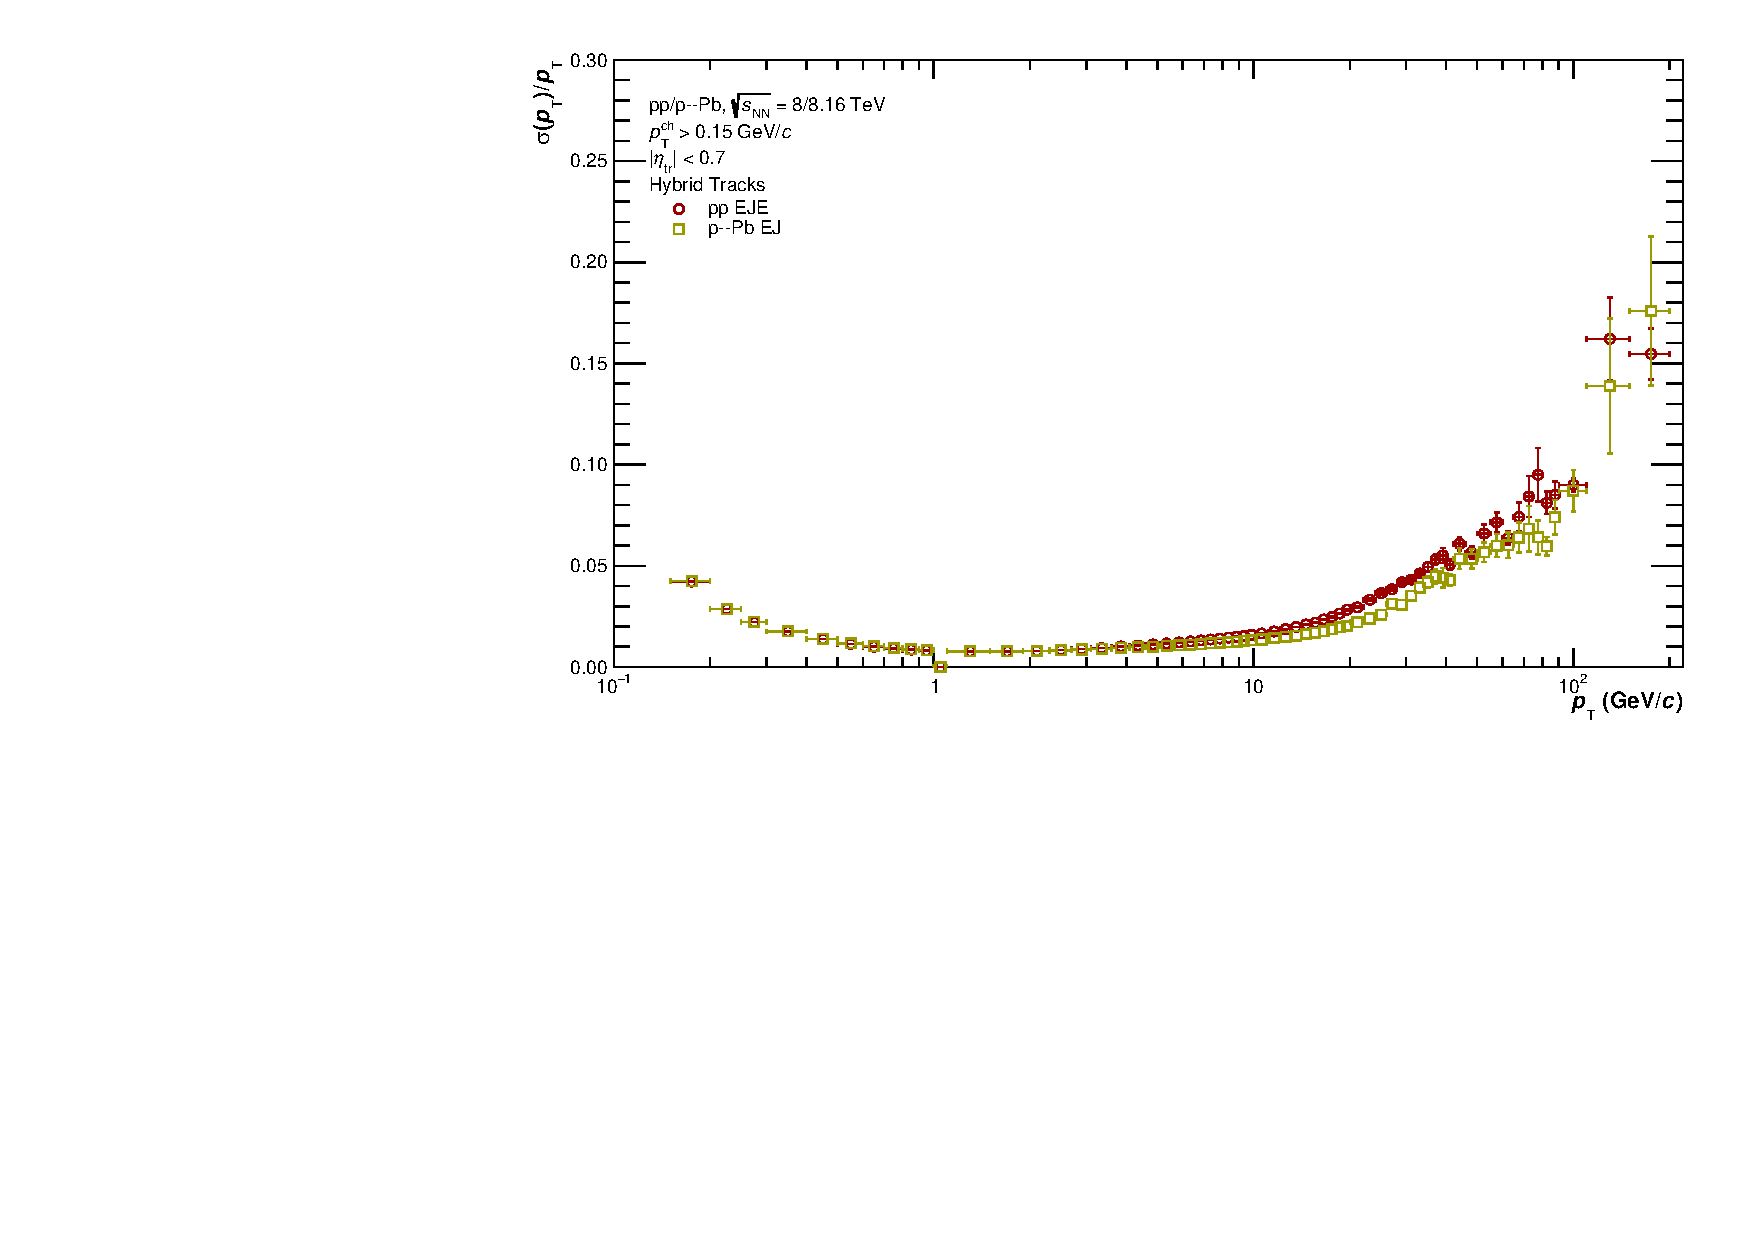
\includegraphics[width=\textwidth]{figures/TrackingQA/PtResolution/PtRes_ppVSpPb.pdf}
    \caption{Transverse momentum resolution for tracks in \pp and \pPb collisions in EMCal jet triggered events.}
    \label{fig:ptresolution}
\end{figure}

\subsection{EMCal Clusters}
\label{sec:ClusterSelection}

When a particle hits the EMCal, it will induce a shower that is primarily contained in one EMCal cell, but spreads out to adjacent cells. These cells must be combined through a process called clusterization in order to reconstruct the full particle energy. The primary cell must pass a specified seed threshold, and then cells are added to the cluster until no adjacent cell above the specified cell threshold remains.

EMCal clusters reconstructed with the v3-clusterizer algorithm are required to have a minimum energy of 300 MeV. Additional corrections for clusters reconstructed in the EMCal can be found in the recent EMCal performance paper~~\cite{EMCalPerformance2022}. Particles from multiple bunch crossings can be recorded in the same event. This includes event pileup and slowly propagating particles such as slow neutrons. In order to remove clusters from different bunch crossings within the EMCal integration window, only energy deposits within [-30,+35] ns for \pp and [-50,+50] ns for \pPb with respect to the measured bunch crossing time are considered. These are the cuts used within the GA group, and the same was followed here. Cluster energy measured before the event cannot be from the event, given a finite resolution, and are concluded to be from beam-gas interactions or event pileup. Cluster energy measured after the event arises from beam-gas interactions or slower particles that take longer to propagate through the detectors. 

In order to avoid double counting of energy deposited by charged particles in the EMCal, the contribution from all tracks matched to clusters is estimated and subtracted from the cluster energy using momentum-dependent track matching. Exotic clusters, i.e clusters with a very high percentage of energy deposited in a single cell due to a high-energy particle hitting one of the avalanche photodiodes, are removed from the analysis. EMCal clusters are accepted up to an energy of 200 GeV. Above this energy, the response of the EMCal is substantially non-linear and is not well understood (see Figure~\ref{fig:emcal_testbeam}). Clusters are corrected for non-linearity using the final corrections stated in the recent EMCal performance paper \cite{EMCalPerformance2022}. This corresponds to kTestBeamShaper and kTestBeamFinalMC for data and monte carlo, respectively. The maximum cluster energy is also varied in the systematic uncertainties to account for this effect. The EMCal trigger cluster yields for all three triggers in \pp collisions are shown in Figure~\ref{fig:triggerClusters_pp}, given for jet resolution parameter $R$ = 0.2. The same is shown for \pPb collisions in Figure~\ref{fig:triggerClusters_pPb}. The cluster and jet yields from each trigger are at different scales due to the downscaling of the minimum bias, EMC7, and EJ2 triggers to different degrees in order to allow trigger time for the EMCal triggers to record rare events such as jets. This scaling must be corrected before the results from different event triggers are combined. As the integrated luminosity is independent of the probe, the scaling can be determined solely based on the EMCal clusters regardless of the jet reconstruction algorithm.


\begin{figure}[hbt!]
    \centering
    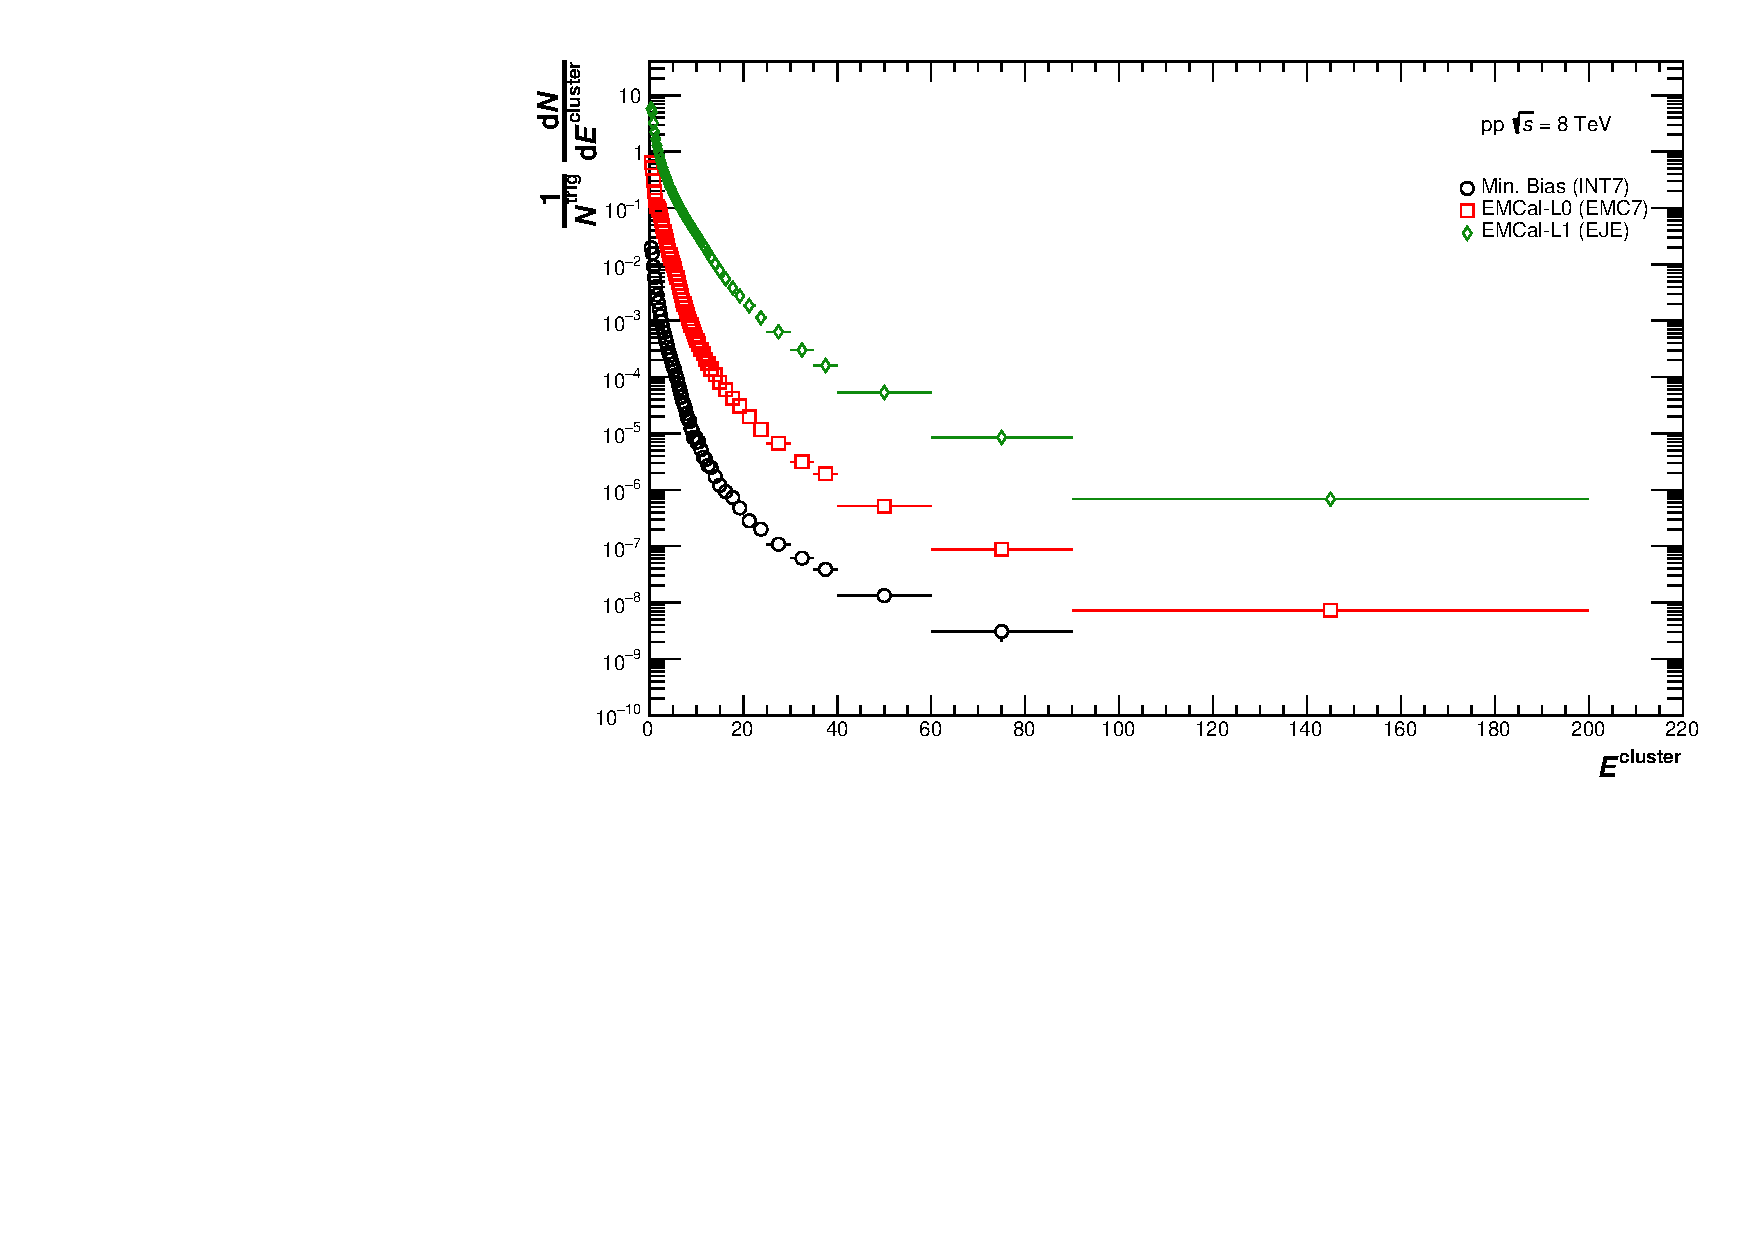
\includegraphics[width=15cm]{figures/TriggerClusters/clusters_R02.pdf}
    \caption{Trigger cluster yields for the INT7, EMC7, and EJE triggers in \pp. Scaling by the rejection factor is required in order for the spectra to overlap.}
    \label{fig:triggerClusters_pp}
\end{figure}

\begin{figure}[hbt!]
    \centering
    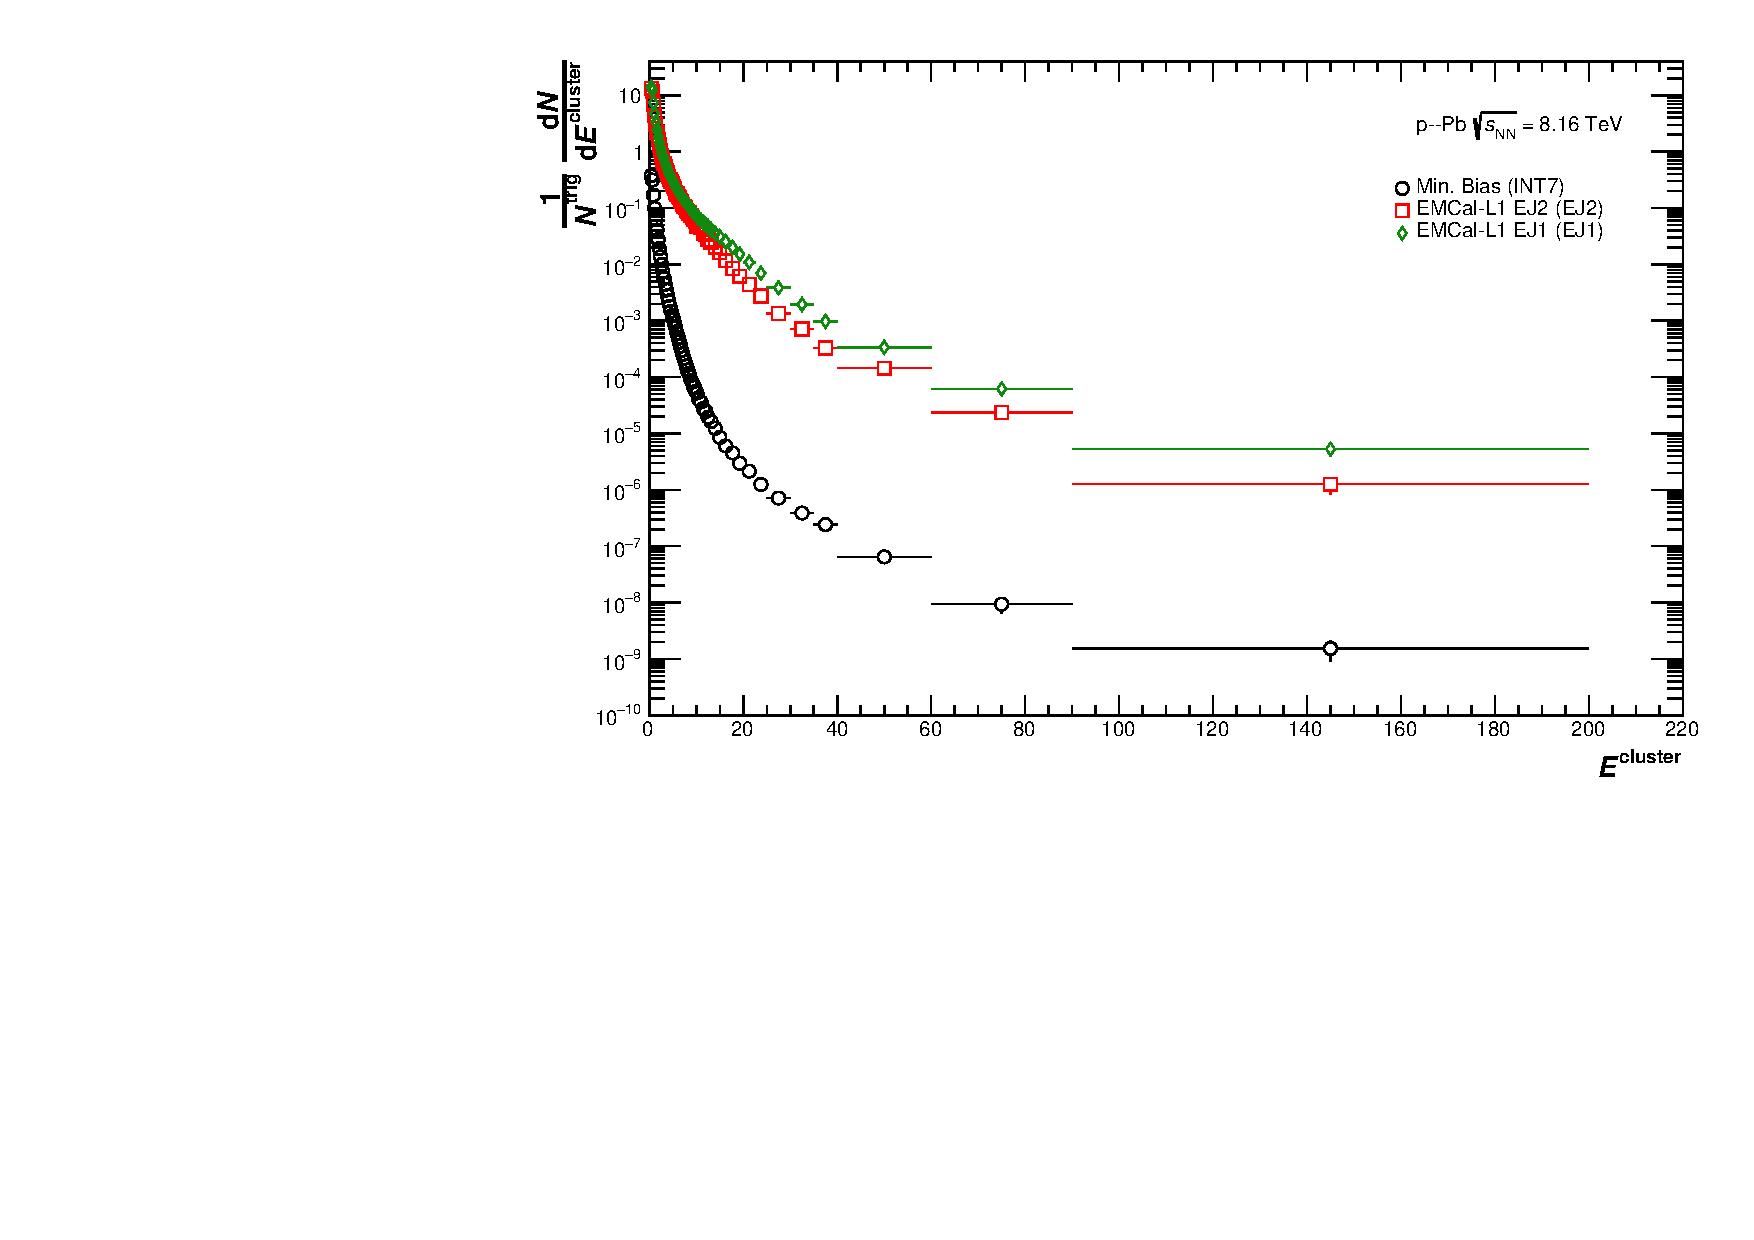
\includegraphics[width=15cm]{figures/pPbFigures/TriggerClusters/clusters_R02.pdf}
    \caption{Trigger cluster yields for the INT7, EJ2, and EJ1 triggers in \pPb. Scaling by the rejection factor or by the trigger luminosity is required in order for the spectra to overlap.}
    \label{fig:triggerClusters_pPb}
\end{figure}

\subsection{Jets}
\label{sec:JetSelection}

Jets are reconstructed using the anti-k$_T$ algorithm~\cite{Cacciari:2008gp} under the \pT-scheme using the FastJet~\cite{Cacciari:2011ma} package. These methods for track, cluster and jet selection were also used in previous measurements, such as in Ref.~\cite{anaNoteMFasel}, and are standard for jet analyses in ALICE. Jets are required to be fully contained within the EMCal acceptance and have a minimum \pT of 10 GeV/$c$. Jets are reconstructed with a resolution parameter defined as $R = \sqrt{(\Delta\eta)^2 + (\Delta\phi)^2}$. The area of the jet must pass the cut $A_{jet} > 0.6\pi R^2$ to suppress background, where $\pi R^2$ is the area of a jet cone with resolution parameter $R$. After all cuts have been applied, the average number of both tracks and clusters in a jet is around 3 to 4 tracks/clusters in the low \pT range of the measurement and around 8 to 9 tracks/clusters in the high \pT range of the measurement. These numbers hold for both \pp and \pPb collisions.

The selected jet \pT ranges for \pp collisions are 20 to 240 GeV/$c$ for jet radii R = 0.2 to 0.5 and 20 to 160 GeV/$c$ for R = 0.6, where the statistics in the highest bins limit the extent of the spectrum. For \pPb collisions, the range for R = 0.2 to 0.4 is 20 to 240 GeV/$c$, while R = 0.5 is limited to 20 to 120 GeV/$c$. R = 0.6 is not included in the \pPb analysis due to a lack of statistics for the entire \pT range. The jet \pT ranges along with trigger patch sizes and thresholds can be found in Table~\ref{tab:trigger_ranges}.


\begin{table}[hbt!]
    \centering
    \caption{EMCal trigger thresholds, patch sizes, and momentum ranges for different triggers in \pp and \pPb collisions. The lower value in brackets refers to the limit at large jet radii.}
    \begin{tabular}{  m{2cm} | m{3.2cm} | m{3.2cm} | m{3.2cm} | m{3.2cm}  }
        \hline
        System & Trigger Name & Momentum Range (GeV/$c$) & Patch Size (cells) & Threshold (GeV) \\
        \hline
        \pp & INT7 & 20--30 & & \\
            & EMC7 & 30--50 & 4x4 & 2.067 \\
            & EJE & 50--[240/160] & 32x32 & 15.6 \\
        \hline
        \pPb & INT7 & 20--30 & & \\
             & EJ2 & 30--50 & 32x32 & 18 \\
             & EJ1 & 50--[240/120] & 32x32 & 23 \\
        \hline
    \end{tabular}
    \label{tab:trigger_ranges}
\end{table}

% For thesis presentation only:
\iffalse
\begin{table}[hbt!]
    \centering
    \begin{tabular}{  m{2cm} | m{3.2cm} | m{3.2cm} | m{3.2cm} | m{3.2cm}  }
        \hline
        System & Trigger Name & Momentum Range (GeV/$c$) & Threshold (GeV), Patch Size (cells) & $\mathscr{L}_{\text{int}}  (\text{nb}^{-1})$ \\
        \hline
        \pp   & INT7 (Min Bias) & \textbf{20}--30 & & 1.03 \\
        8 TeV & EMC7 (EMCal $\gamma$) & 30--60 & 2.076, 4x4 & 41.4 \\
              & EJE (EMCal Jet) & 60--\textbf{[240/160]} & 15.6, 32x32 & 8.75 \\
        \hline
        \pPb     & INT7 (Min Bias) & \textbf{20}--30 & & 7.35$\times 10^{-3}$ \\
        8.16 TeV & EJ2 (EMCal Jet) & 30--50 & 18, 32x32 & 6.51$\times 10^{-2}$ \\
                 & EJ1 (EMCal Jet) & 50--\textbf{[240/120]} & 23, 32x32 & 1.34 \\
        \hline
    \end{tabular}
\end{table}
\fi

\subsection{Bias of the EMCal Trigger}
\label{sec:EMCTriggerBias}

The EMCal measures all interacting particles, including photons, leptons, and hadrons. Photons can originate directly from the primary vertex, but come primarily from the decay of neutral hadrons such as the $\pi^0$ meson. Hadrons that interact directly with the calorimeter include those which leave minimal ionization energy and those which interact hadronically and leave a partial shower. Since the matched tracks are subtracted off if they are matched to an EMCal cluster, a large portion of the remaining particles are photons. For this reason, it is referred to as the neutral energy fraction (NEF), although the contribution from neutral hadrons interacting directly with the EMCal is small. The neutral energy fraction is the fraction of energy from the track + EMCal cluster composite object coming from the cluster.

The EMCal triggers are used to measure high energy jet events. As the trigger selects jets based on the amount of energy deposited in the calorimeter, it introduces a bias on the jets that vanishes only at higher \pT. Figure~\ref{fig:NEF} shows the comparison of the distribution of the neutral energy fraction for \pp jets in minimum bias and triggered events for various bins in jet \pT for R = 0.2 jets. The distributions are compared to the neutral energy fraction distributions calculated using a PYTHIA8 simulation. For other radii and equivalent plots in \pPb, see Appendix~\ref{sec:appendixTriggerBiaspPb}. Figure~\ref{fig:meanNEF_pp} shows the mean neutral energy fraction in \pp collisions for various jet resolution parameters, and Figure~\ref{fig:meanNEF_pPb} shows the same in \pPb collisions.

For the lowest jet \pT bins, the distributions show significant scale differences. At low \pT, jets in EMCal triggered events are dominated by the neutral component. Jets are required to deposit enough energy in the EMCal to pass the trigger. For jets with a given energy in the low momentum regime close to the trigger threshold, only those that deposit a larger fraction of their energy in the EMCal will pass the threshold. At lower \pT in minimum bias events, an effect is seen from the different track and cluster \pT cutoffs of 150 MeV and 300 MeV. As jet \pT decreases, it is more likely to find jets which are dominated by charged particles as opposed to calorimeter clusters, since the cutoff for tracks is lower. Only for jets with \pT larger than 30 GeV/$c$ for EMC7 and 60 GeV/$c$ for EJE, the distributions for the triggers start overlapping with the distribution in minimum bias events. For \pPb, this occurs at 30 GeV for the EJ2 trigger and 50 GeV for the EJ1 trigger. These effects can also be seen in figure 100 of the 2022 EMCal Performance paper \cite{EMCalPerformance}.

The effect from the trigger bias is also shown in Figure~\ref{fig:trigger_ratios}, the \pT dependence of the jet yield ratio of EMC7/INT7 and EJE/EMC7, which fluctuates with \pT until a plateau is reached at approximately 30 GeV for EMC7 and approximately 60 GeV for EJE. At this point, the trigger approaches maximum efficiency, and the bias is minimized. Jets are selected in triggered events only in this low-bias region. 


\begin{figure}[hbt!]
    \centering
    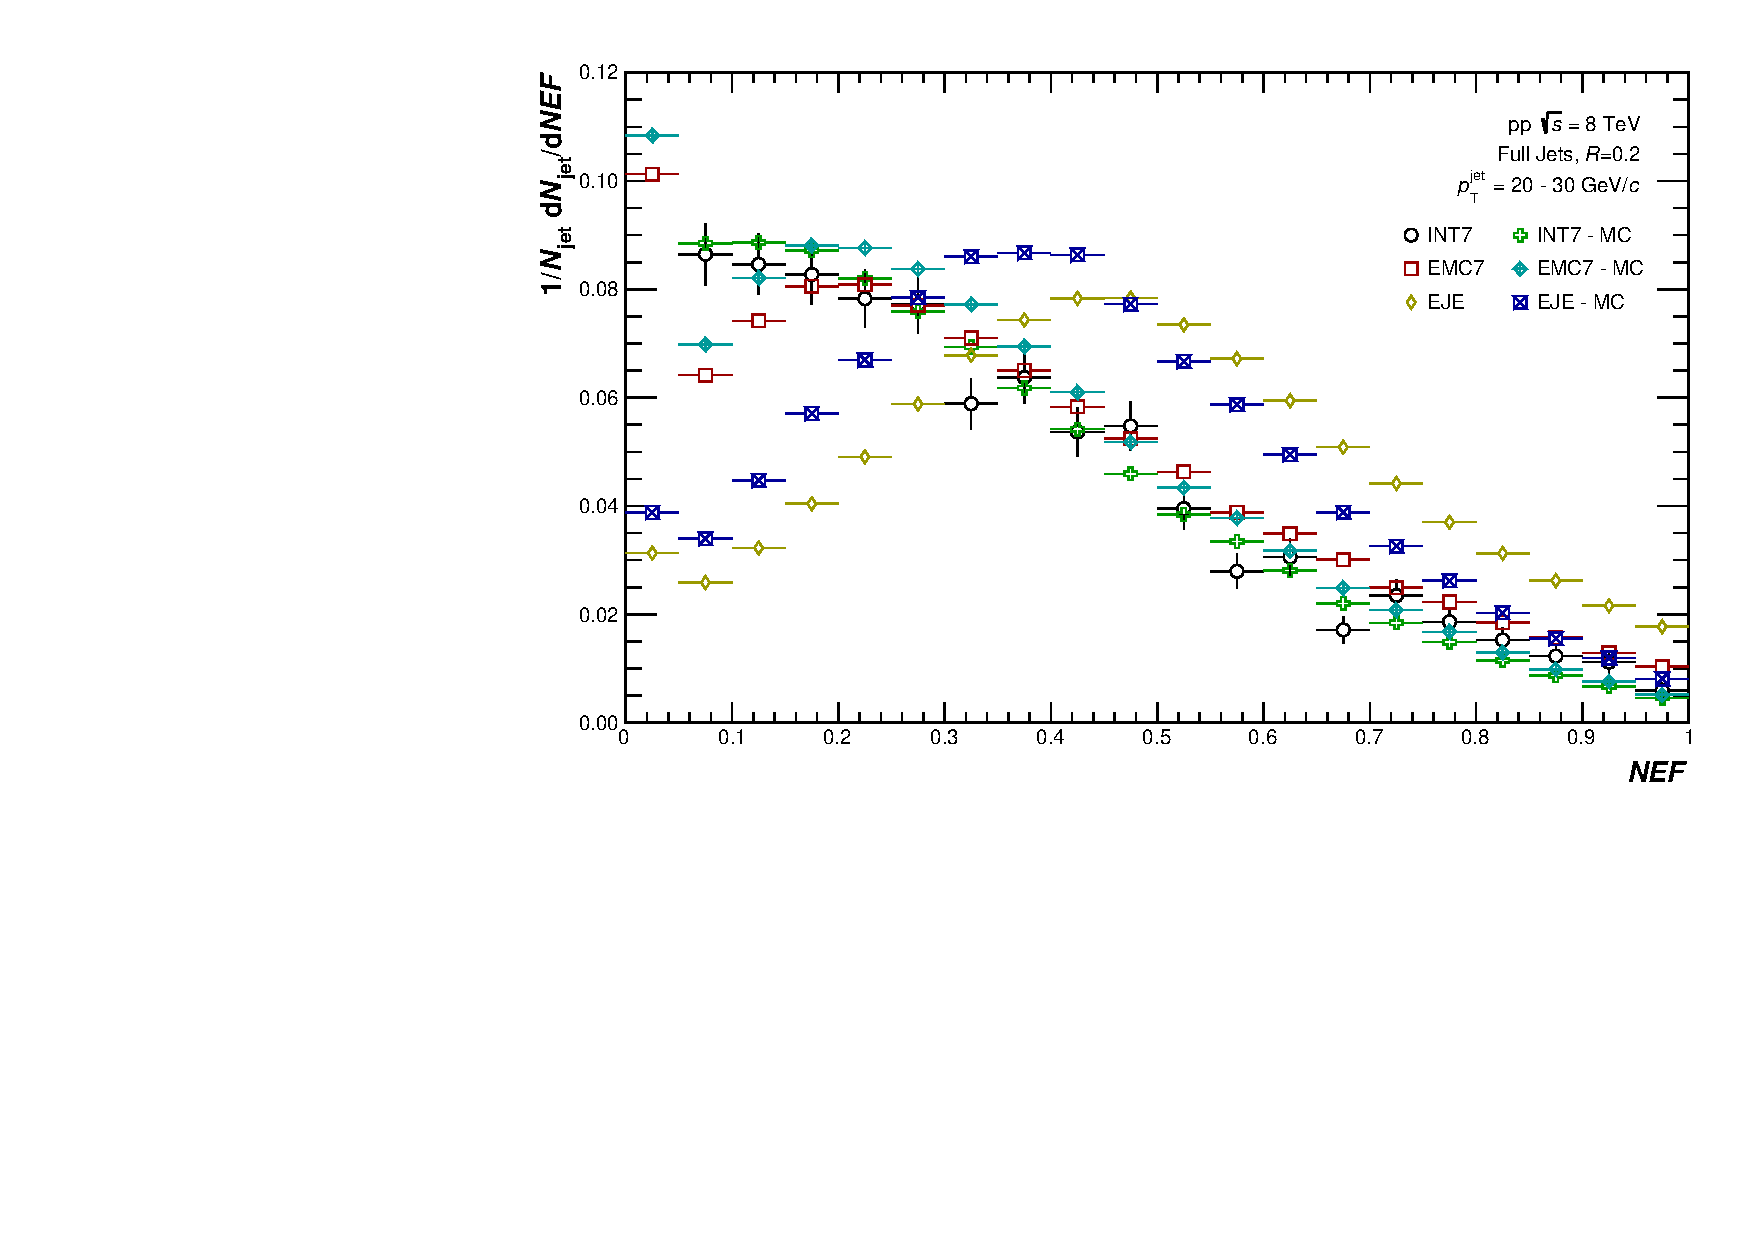
\includegraphics[width=0.49\textwidth]{figures/TriggerBias/NEF/All/hNEF_20-30GeV_R02.pdf}
    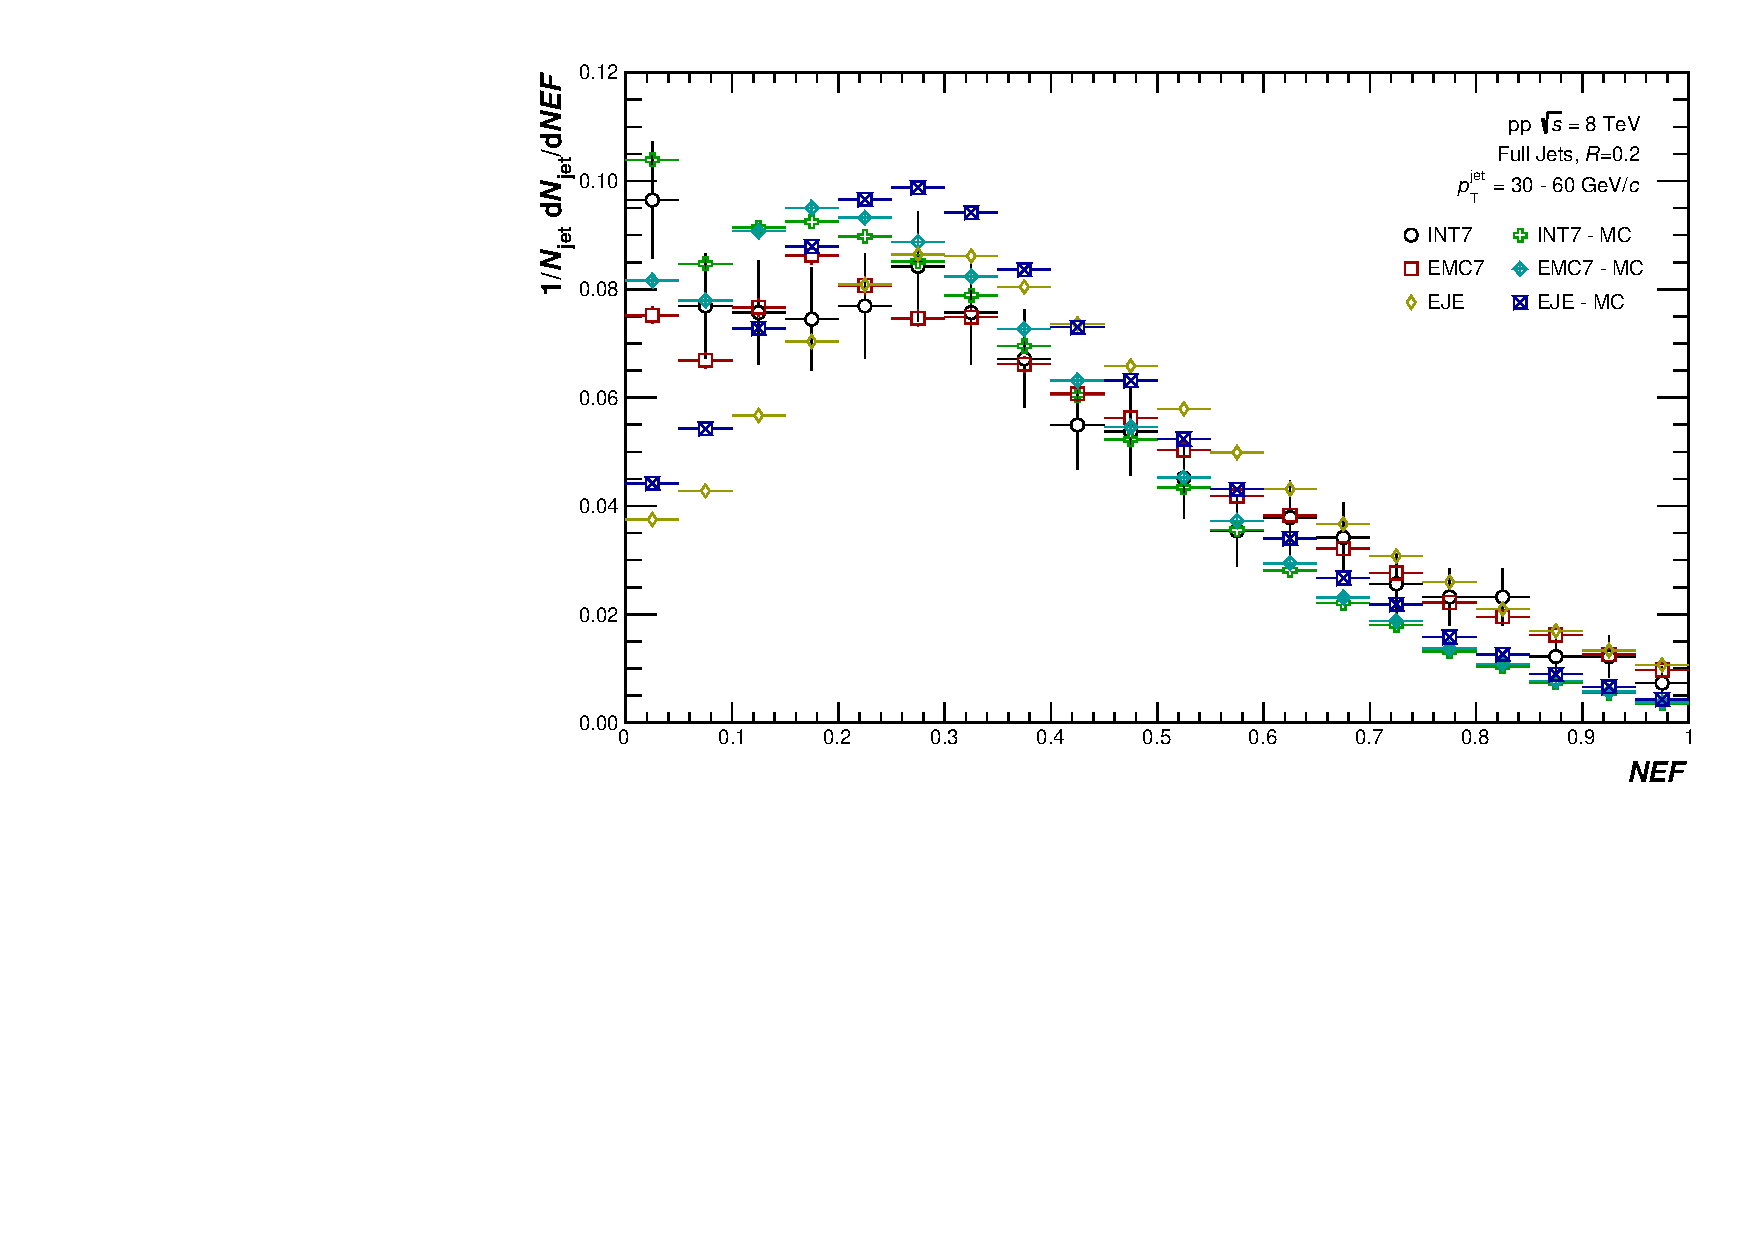
\includegraphics[width=0.49\textwidth]{figures/TriggerBias/NEF/All/hNEF_30-60GeV_R02.pdf}
    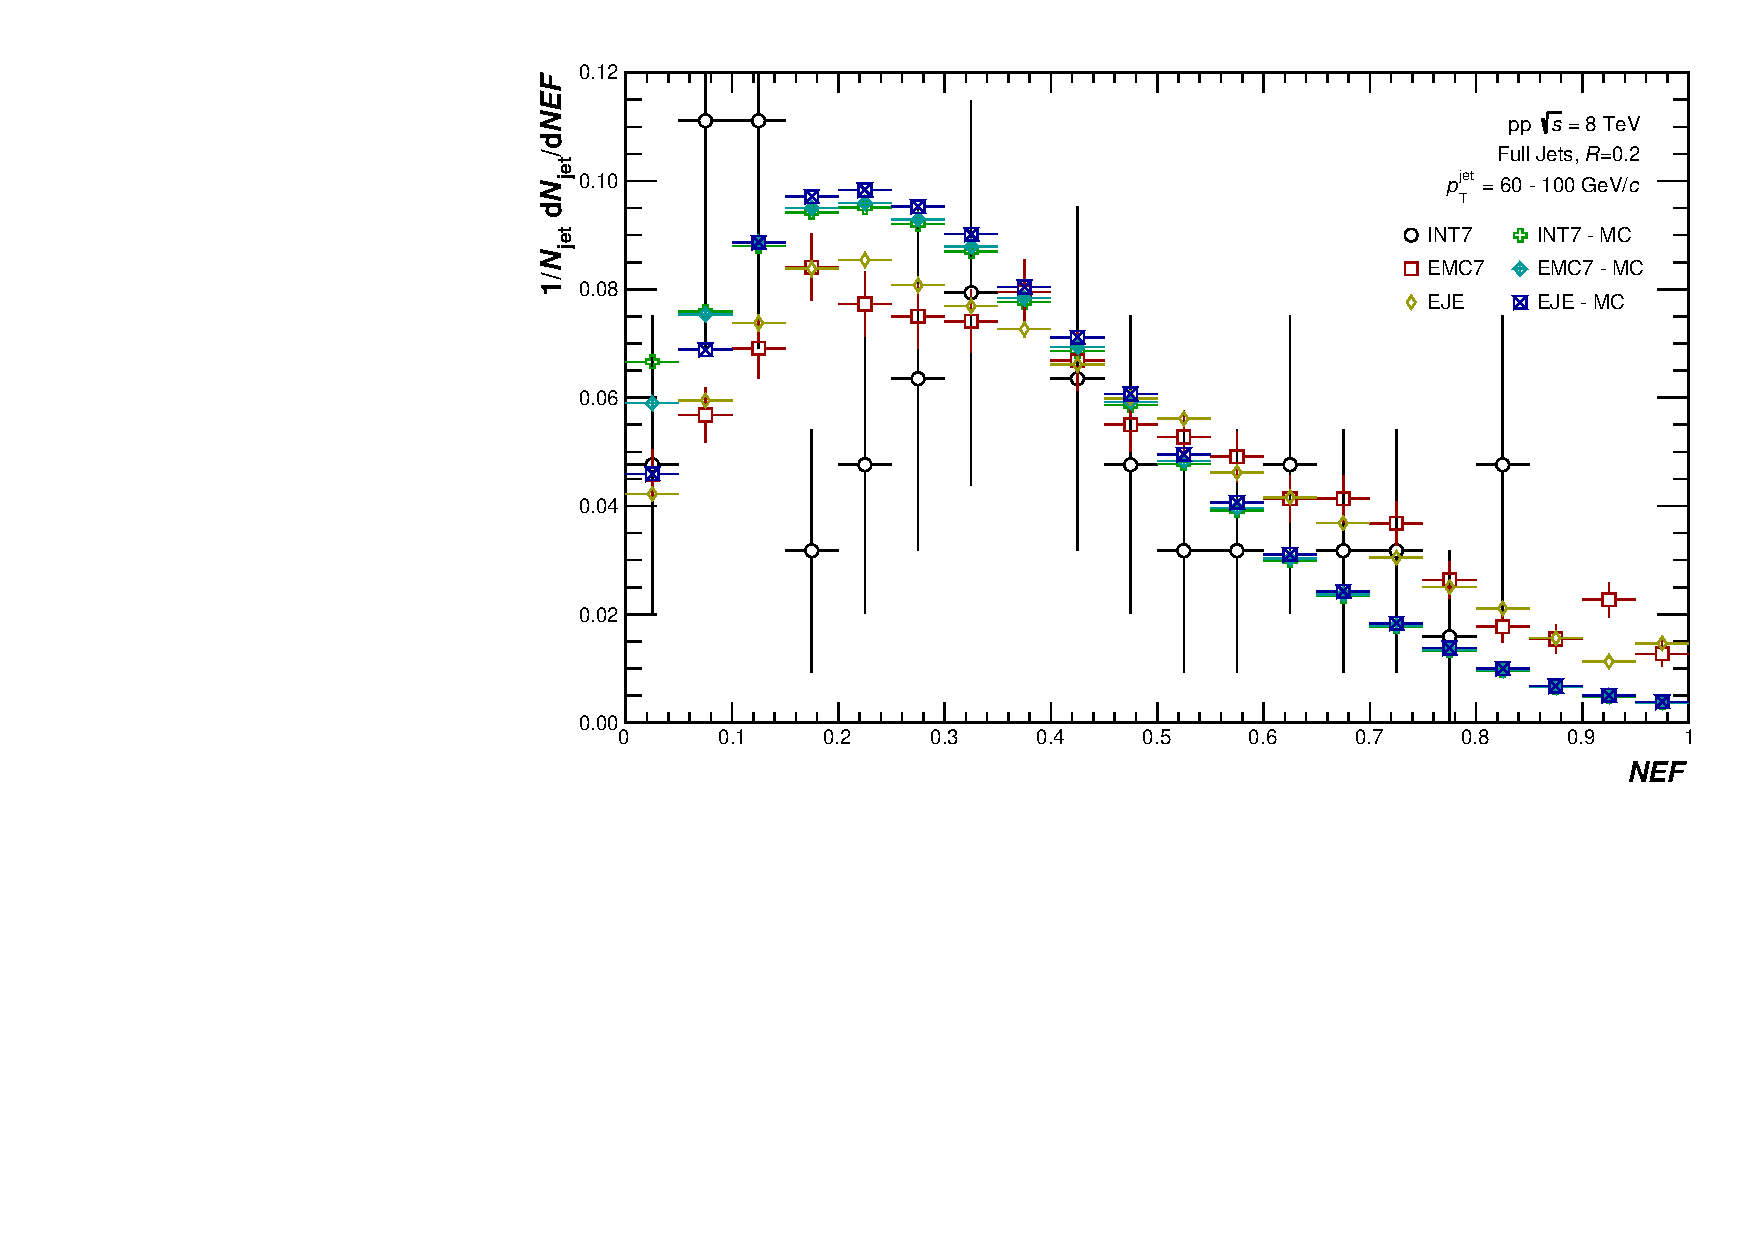
\includegraphics[width=0.49\textwidth]{figures/TriggerBias/NEF/All/hNEF_60-100GeV_R02.pdf}
    \caption{Probability distribution of the neutral energy fraction for jets in \pp collisions in data and PYTHIA8 found using the minimum bias and EMCal triggers for different bins in jet energy using R = 0.2 jets.}
    \label{fig:NEF}
\end{figure}

\begin{figure}[hbt!]
    \centering
    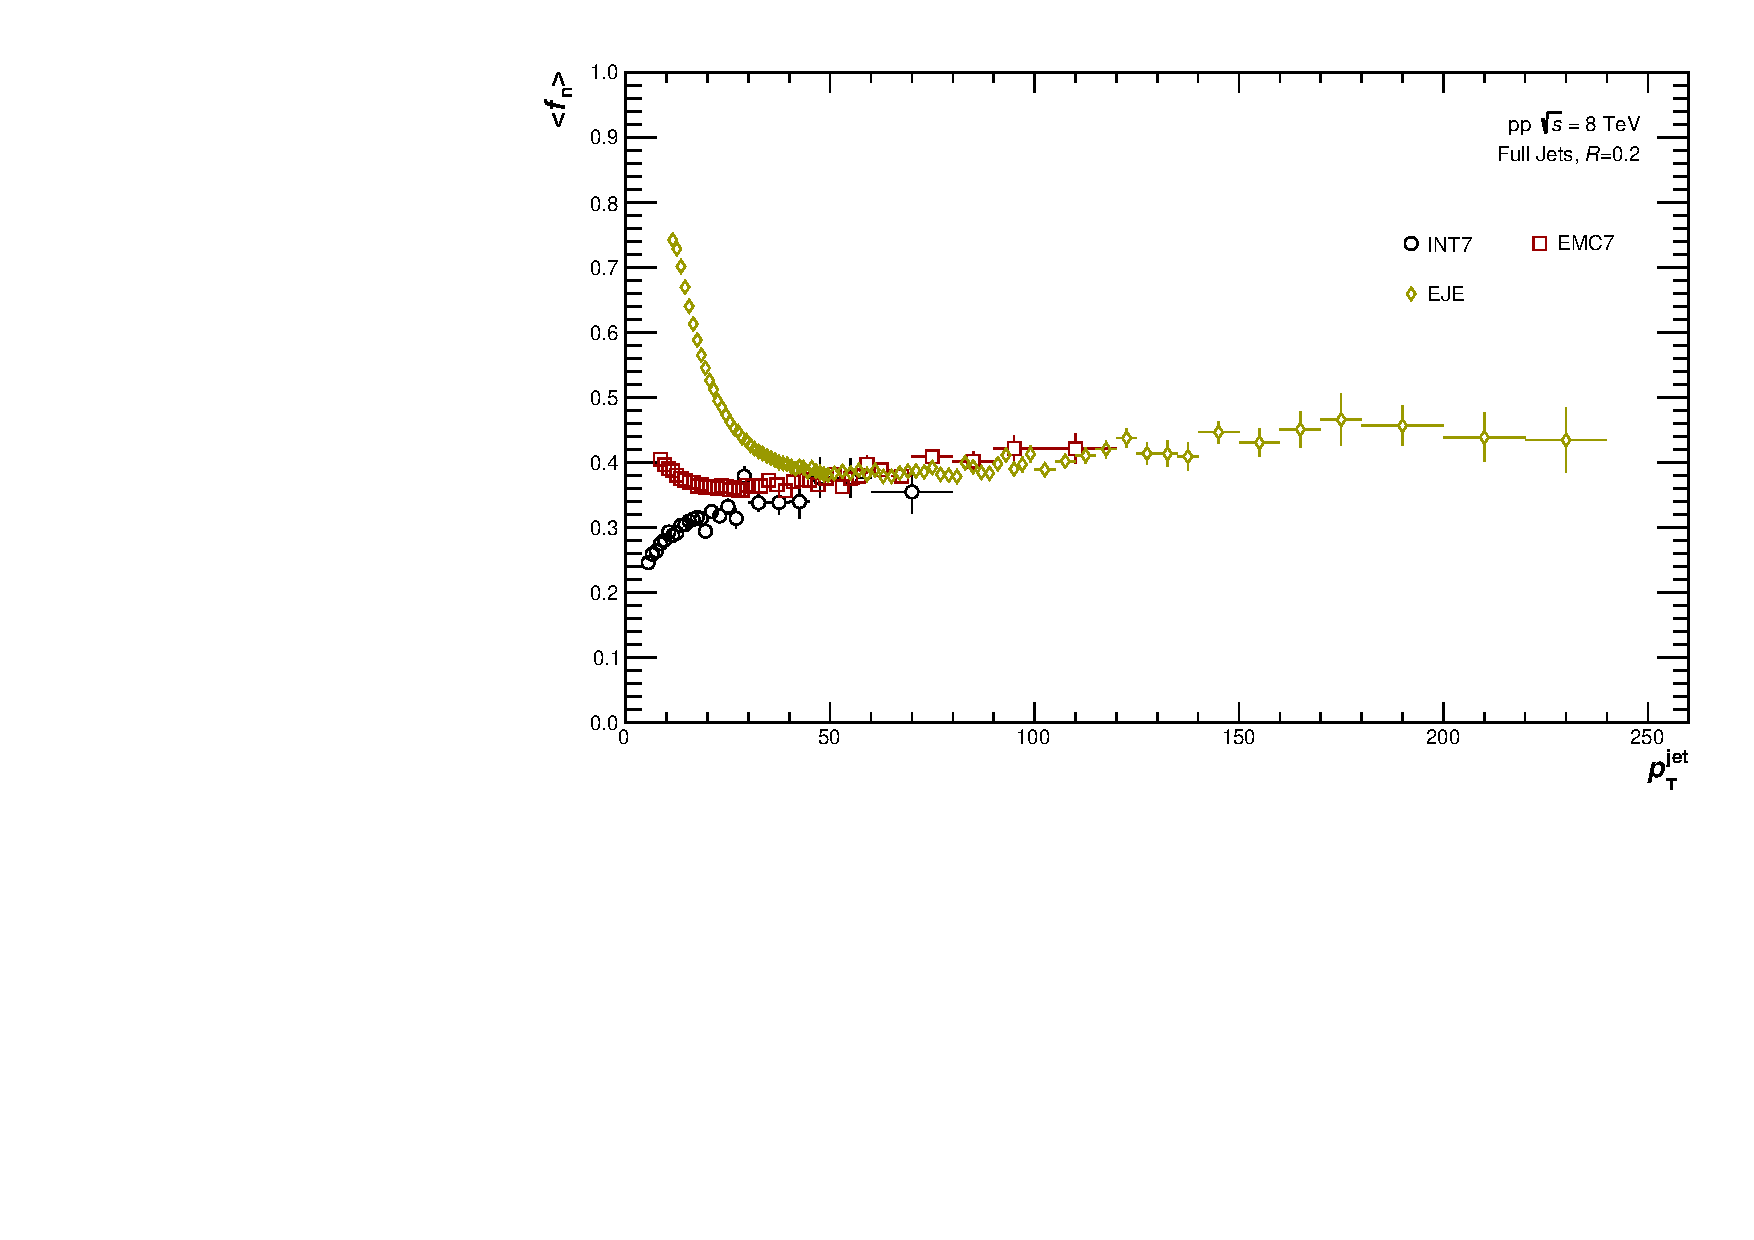
\includegraphics[width=0.49\textwidth]{figures/TriggerBias/NEF/All/mean_NEF_R02.pdf}
    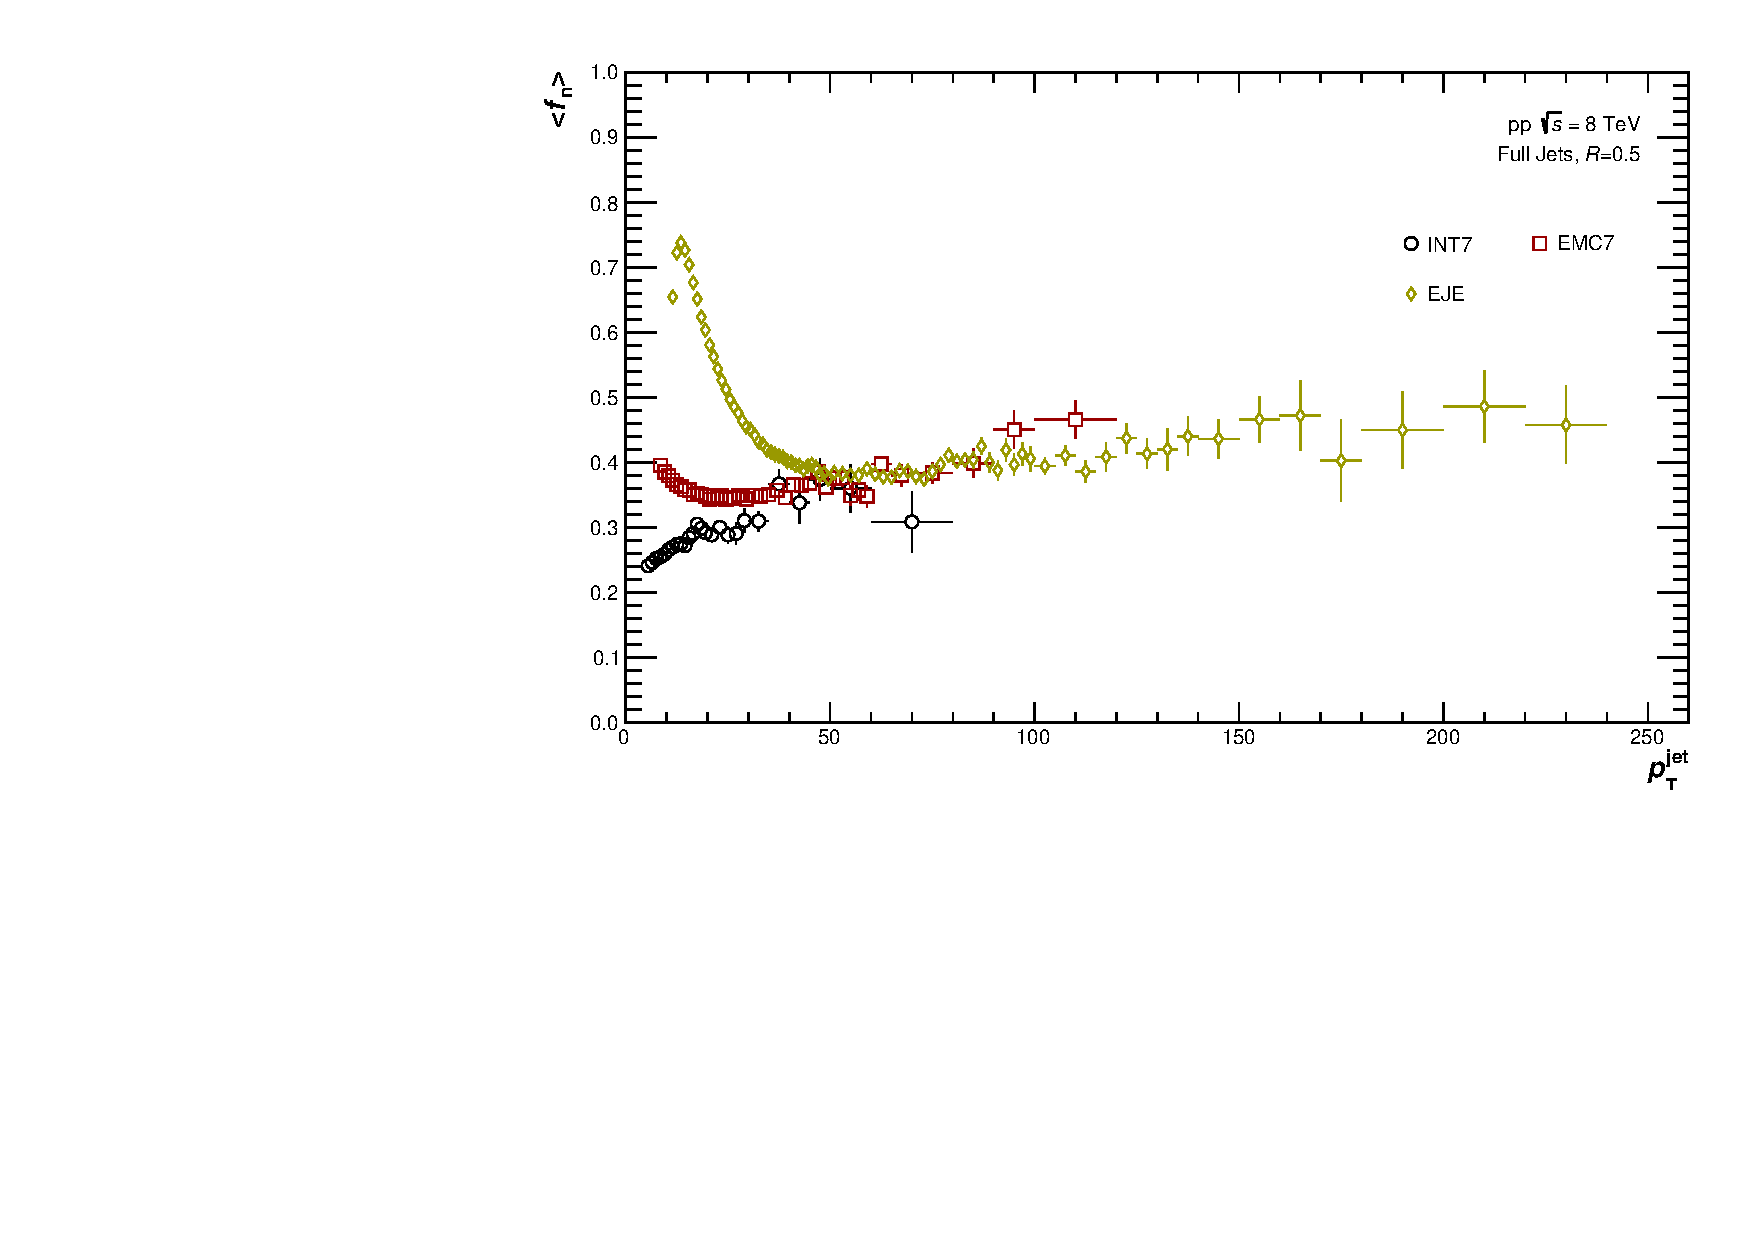
\includegraphics[width=0.49\textwidth]{figures/TriggerBias/NEF/All/mean_NEF_R05.pdf}
    \caption{Mean neutral energy fraction as a function of jet \pT for jets in \pp collisions for minimum bias and EMCal triggers, presented for various jet resolution parameters.}
    \label{fig:meanNEF_pp}
\end{figure}

\begin{figure}[hbt!]
    \centering
    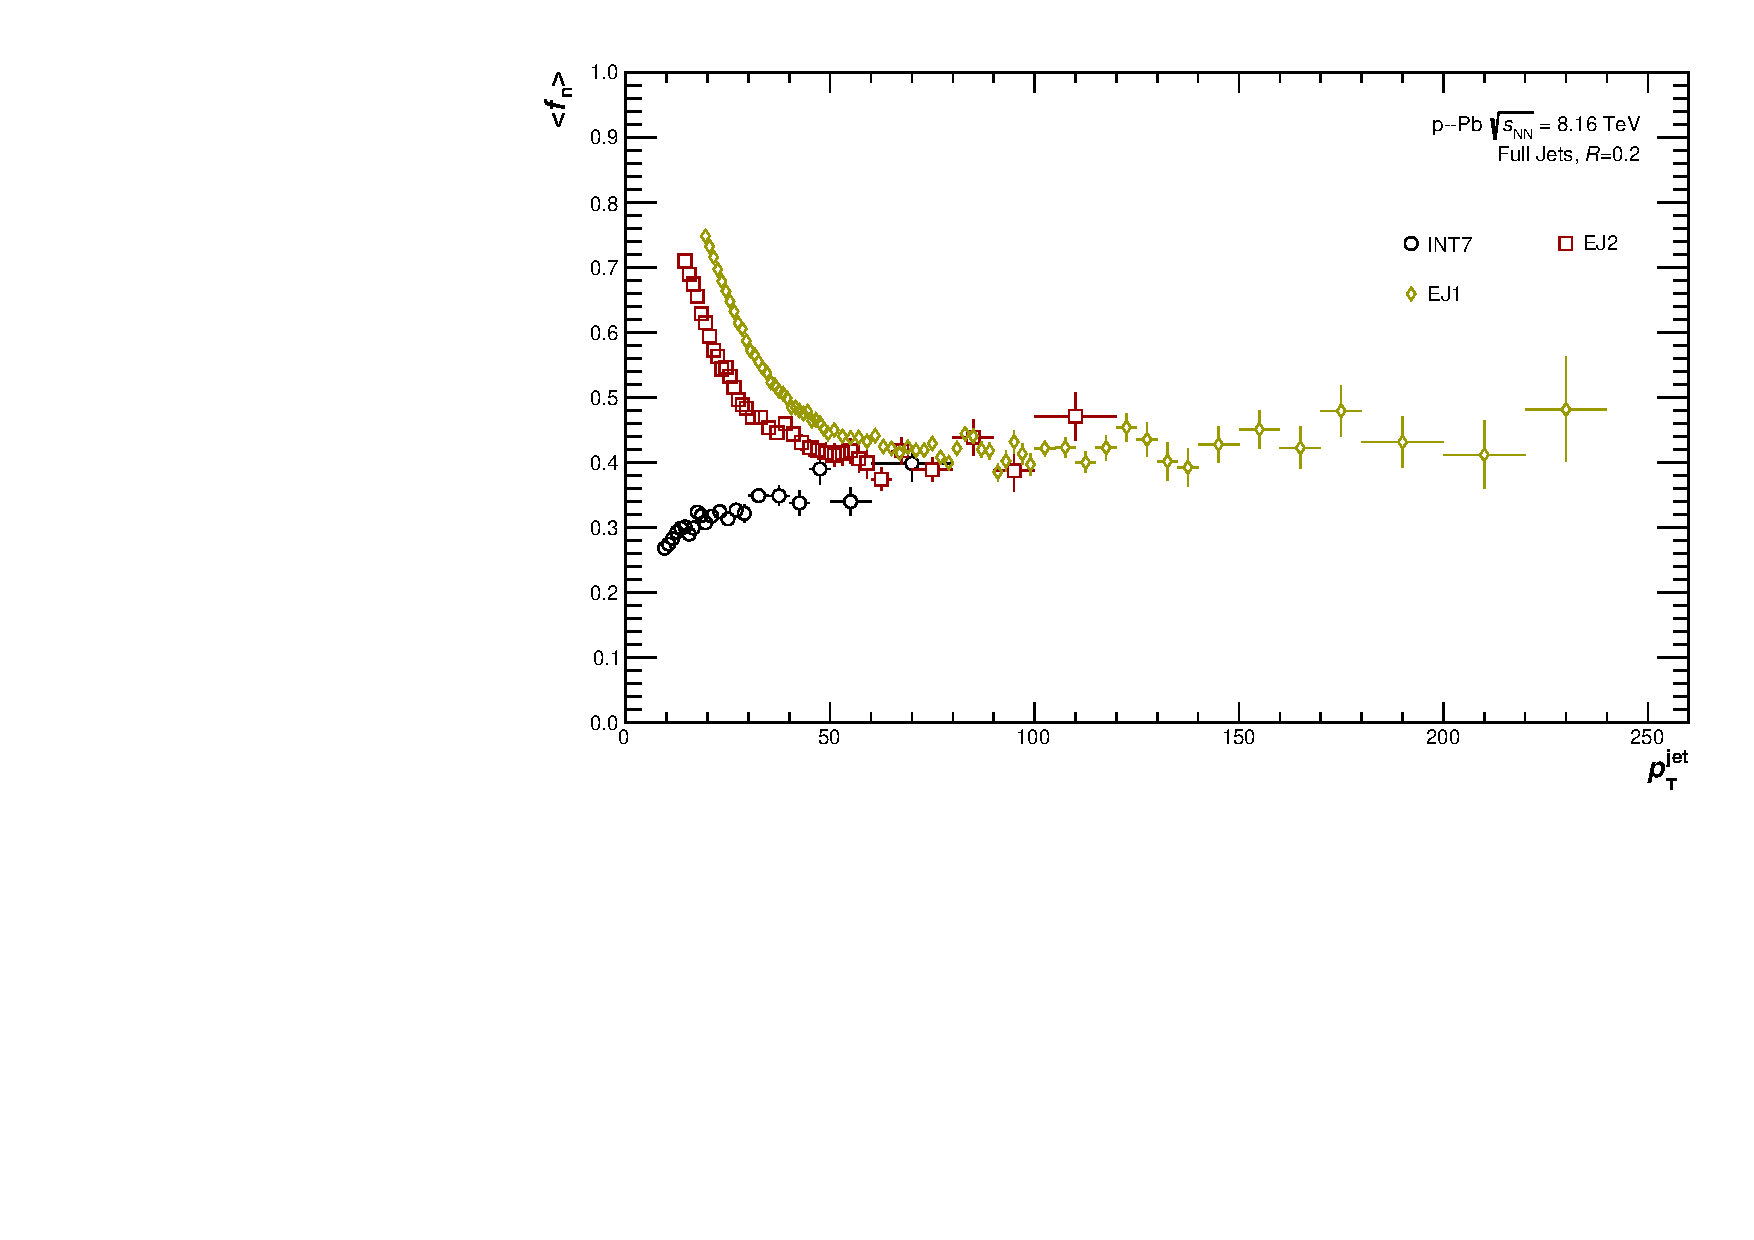
\includegraphics[width=0.49\textwidth]{figures/pPbFigures/TriggerBias/NEF/All/mean_NEF_R02.pdf}
    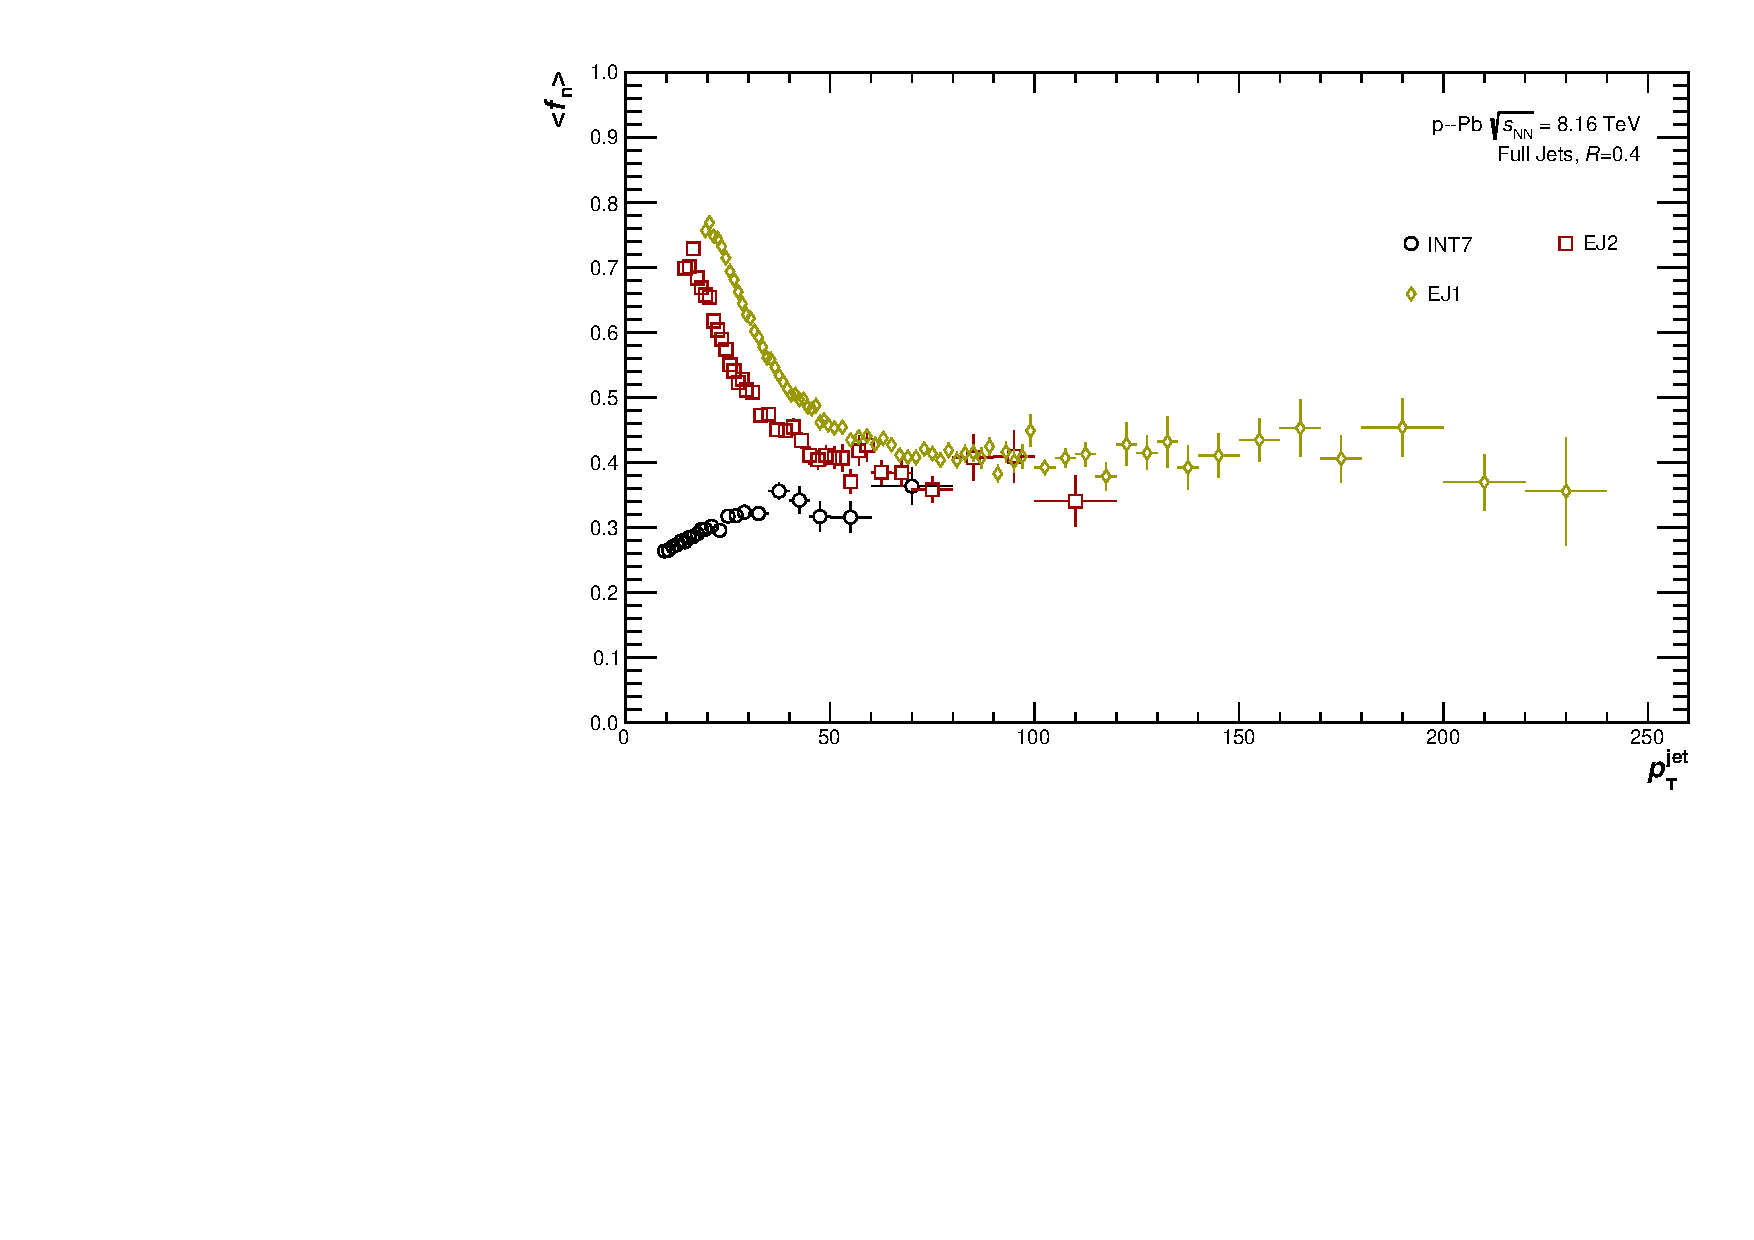
\includegraphics[width=0.49\textwidth]{figures/pPbFigures/TriggerBias/NEF/All/mean_NEF_R04.pdf}
    \caption{Mean neutral energy fraction as a function of jet \pT for jets in \pPb collisions for minimum bias and EMCal triggers, presented for various jet resolution parameters.}
    \label{fig:meanNEF_pPb}
\end{figure}

\begin{figure}[hbt!]
    \centering
    \begin{multicols}{2}
            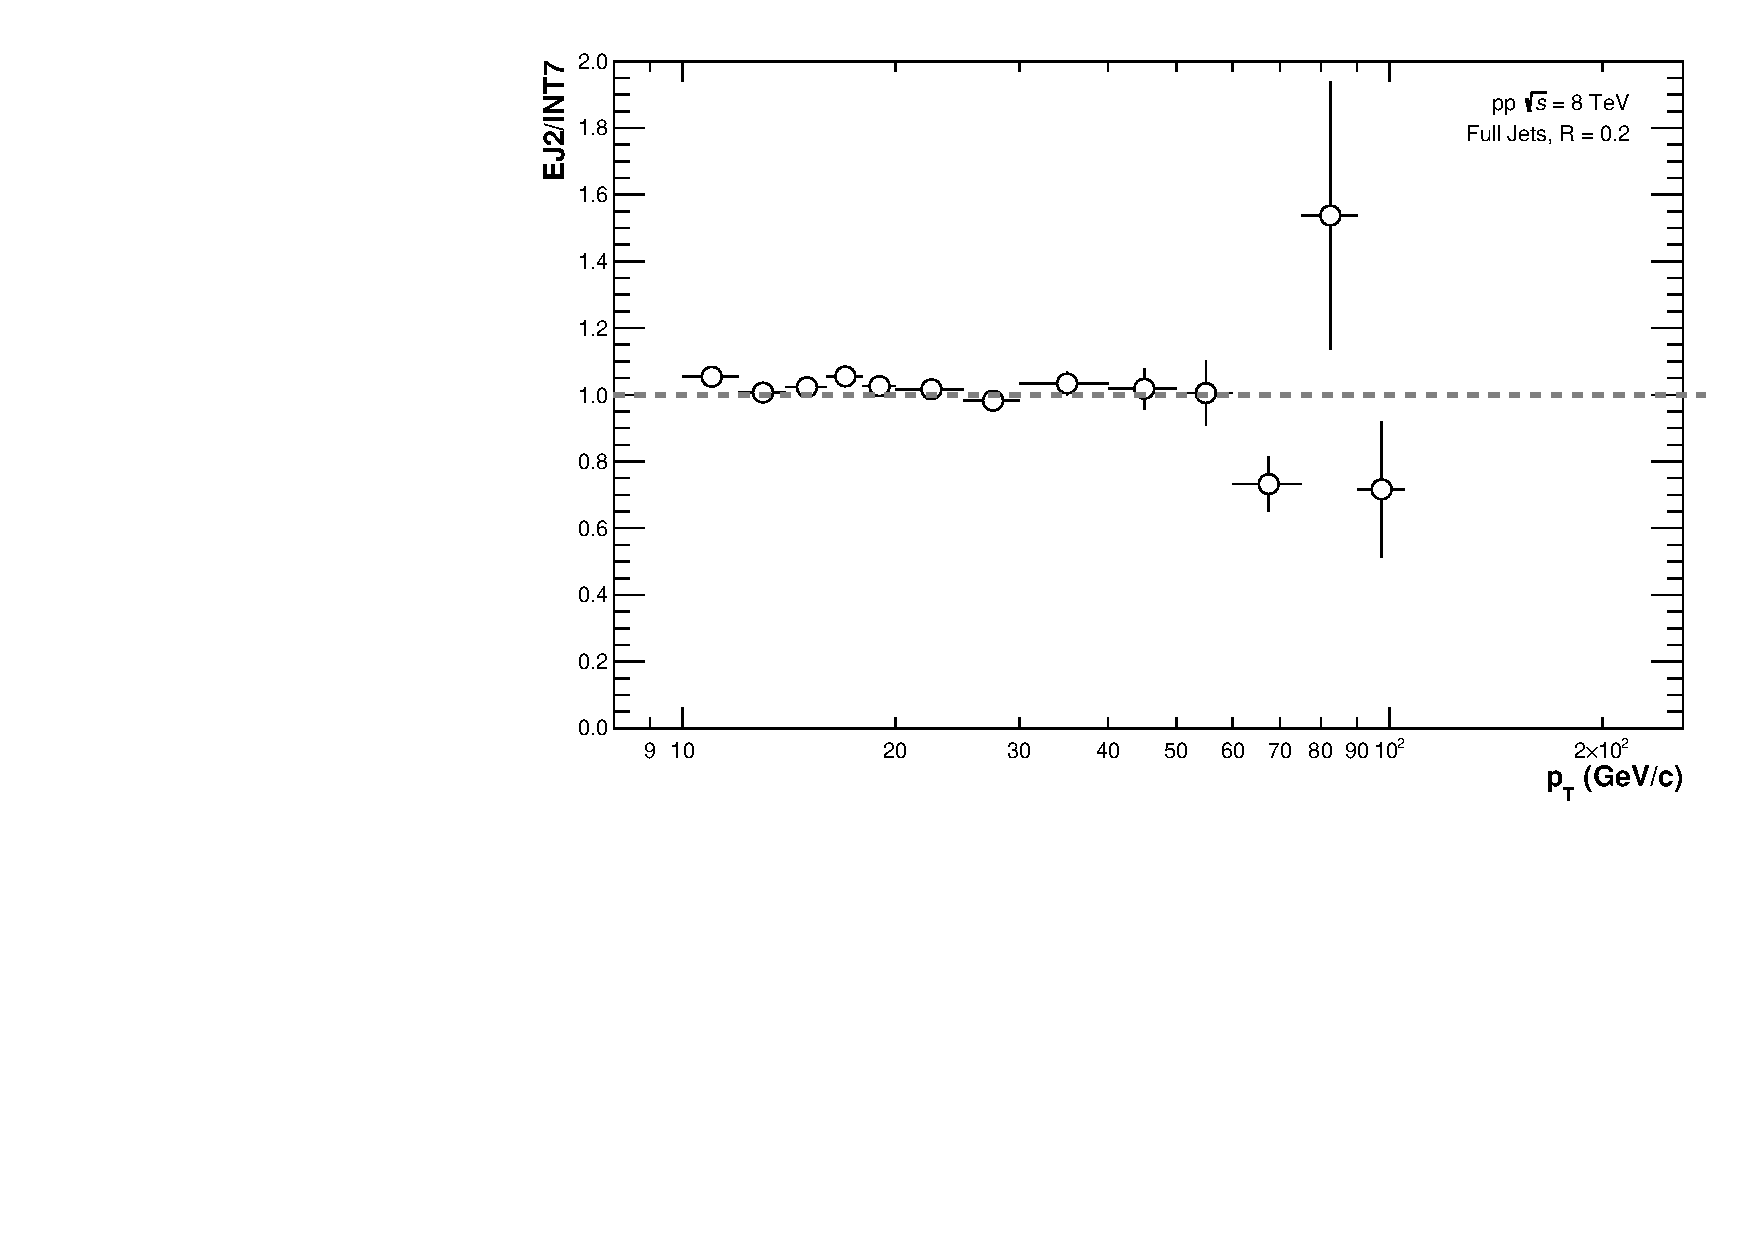
\includegraphics[width=0.49\textwidth]{figures/TriggerSwap/ratio_EMCINT_data_R02.pdf}
        \vfill\null 
        \columnbreak
            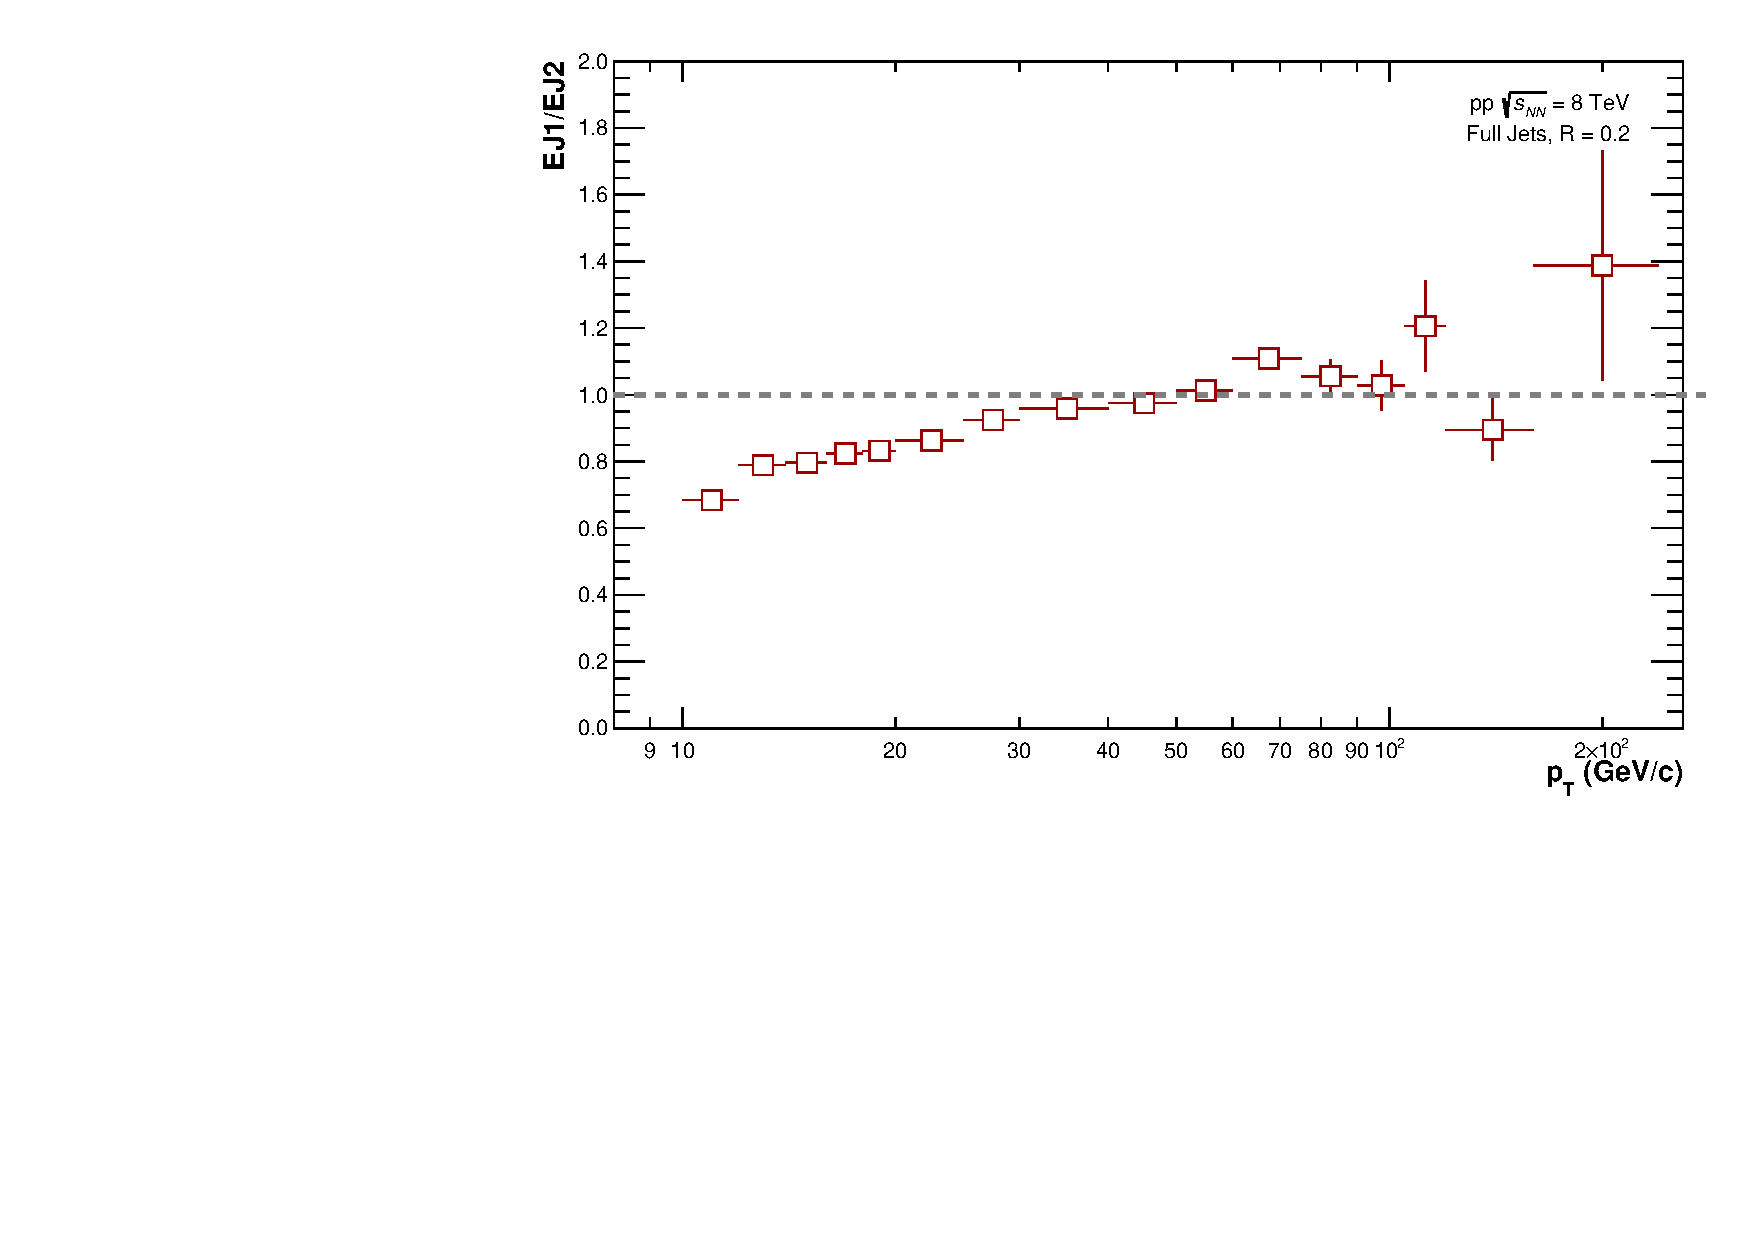
\includegraphics[width=0.49\textwidth]{figures/TriggerSwap/ratio_EJEEMC_data_R02.pdf}
        \vfill\null
    \end{multicols}
    \caption{Ratios of jet yield in \pp data of EMC7/INT7 triggers (left) and EJE/EMC7 triggers (right) as a function of jet \pT.}
    \label{fig:trigger_ratios}
\end{figure}

The trigger response in simulations is obtained by applying the same sliding window algorithm as implemented in the trigger hardware. The trigger uses the raw signal instead of the calibrated signal. Triggered events are required to have at least one trigger patch above the nominal threshold. The accuracy of the trigger bias in simulation is tested by comparing the distributions of the neutral energy fraction, z$_\mathrm{ch}$, and z$_\mathrm{neutral}$ between data and simulation. The observables z$_\mathrm{ch}$ and z$_\mathrm{neutral}$ are the fraction of the jet \pT coming from charged tracks and EMCal clusters. Figure~\ref{fig:TriggerBiasNEFR02} shows the comparison of the neutral energy fraction for jets from \pp collisions with R=0.2 in triggered events between data and simulations for different bins in \pT. The distributions obtained from simulation agree with the distributions obtained from data. 

Figure~\ref{fig:TriggerEfficiency_pp} shows the trigger efficiency for jets with resolution parameter $R$ = 0.2 to 0.5, obtained by taking the ratio of triggered jet spectra to minimum bias jet spectra in simulations of \pp collisions. The trigger becomes fully efficient before reaching the desired ranges of 30 GeV for EMC7 and 60 GeV for EJE. Figure~\ref{fig:TriggerEfficiency_pPb} shows the same in \pPb collisions for jets with resolution parameter $R$ = 0.2 to 0.4. The trigger efficiency never reaches unity but instead plateaus at about 99\% in \pp and about 90\% in \pPb. This is due to the masking of channels at trigger level that are not masked in the front-end readout electronics. Since masking in the front-end electronics is performed at L0, the acceptance is the same for both L0 and L1 trigger levels. Additionally, there are contributions from jets which contain only particles that are never reconstructed, such as $K_L^0$, and from jets that never get matched due to the finite matching efficiency. In the low momentum region, other detector effects which are not simulated (i.e. random noise) play a role and the simulated trigger efficiency will overestimate the correction.


\begin{figure}[hbt!]
    \centering
    \begin{multicols}{2}
            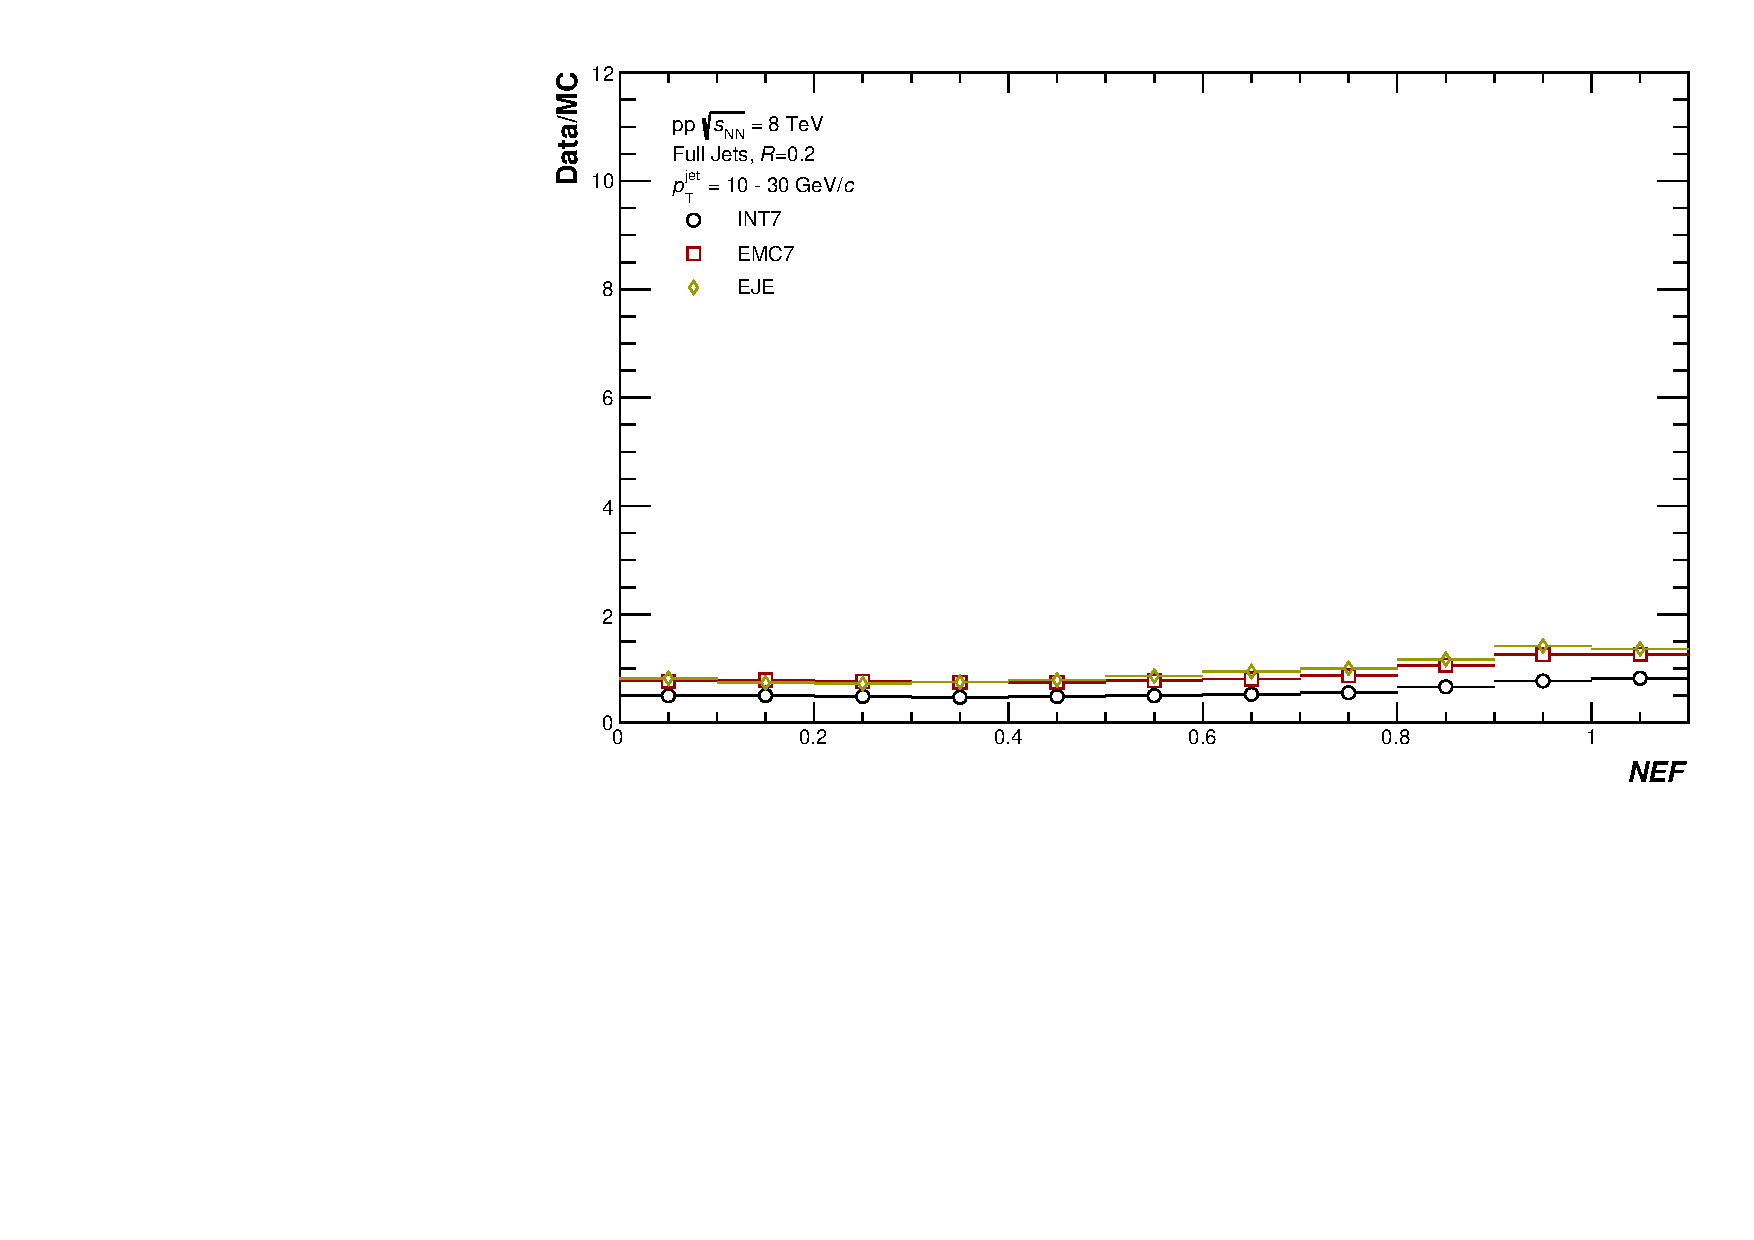
\includegraphics[width=0.49\textwidth]{figures/TriggerBias/NEF/hNEF_ptBin1_R02.pdf}
            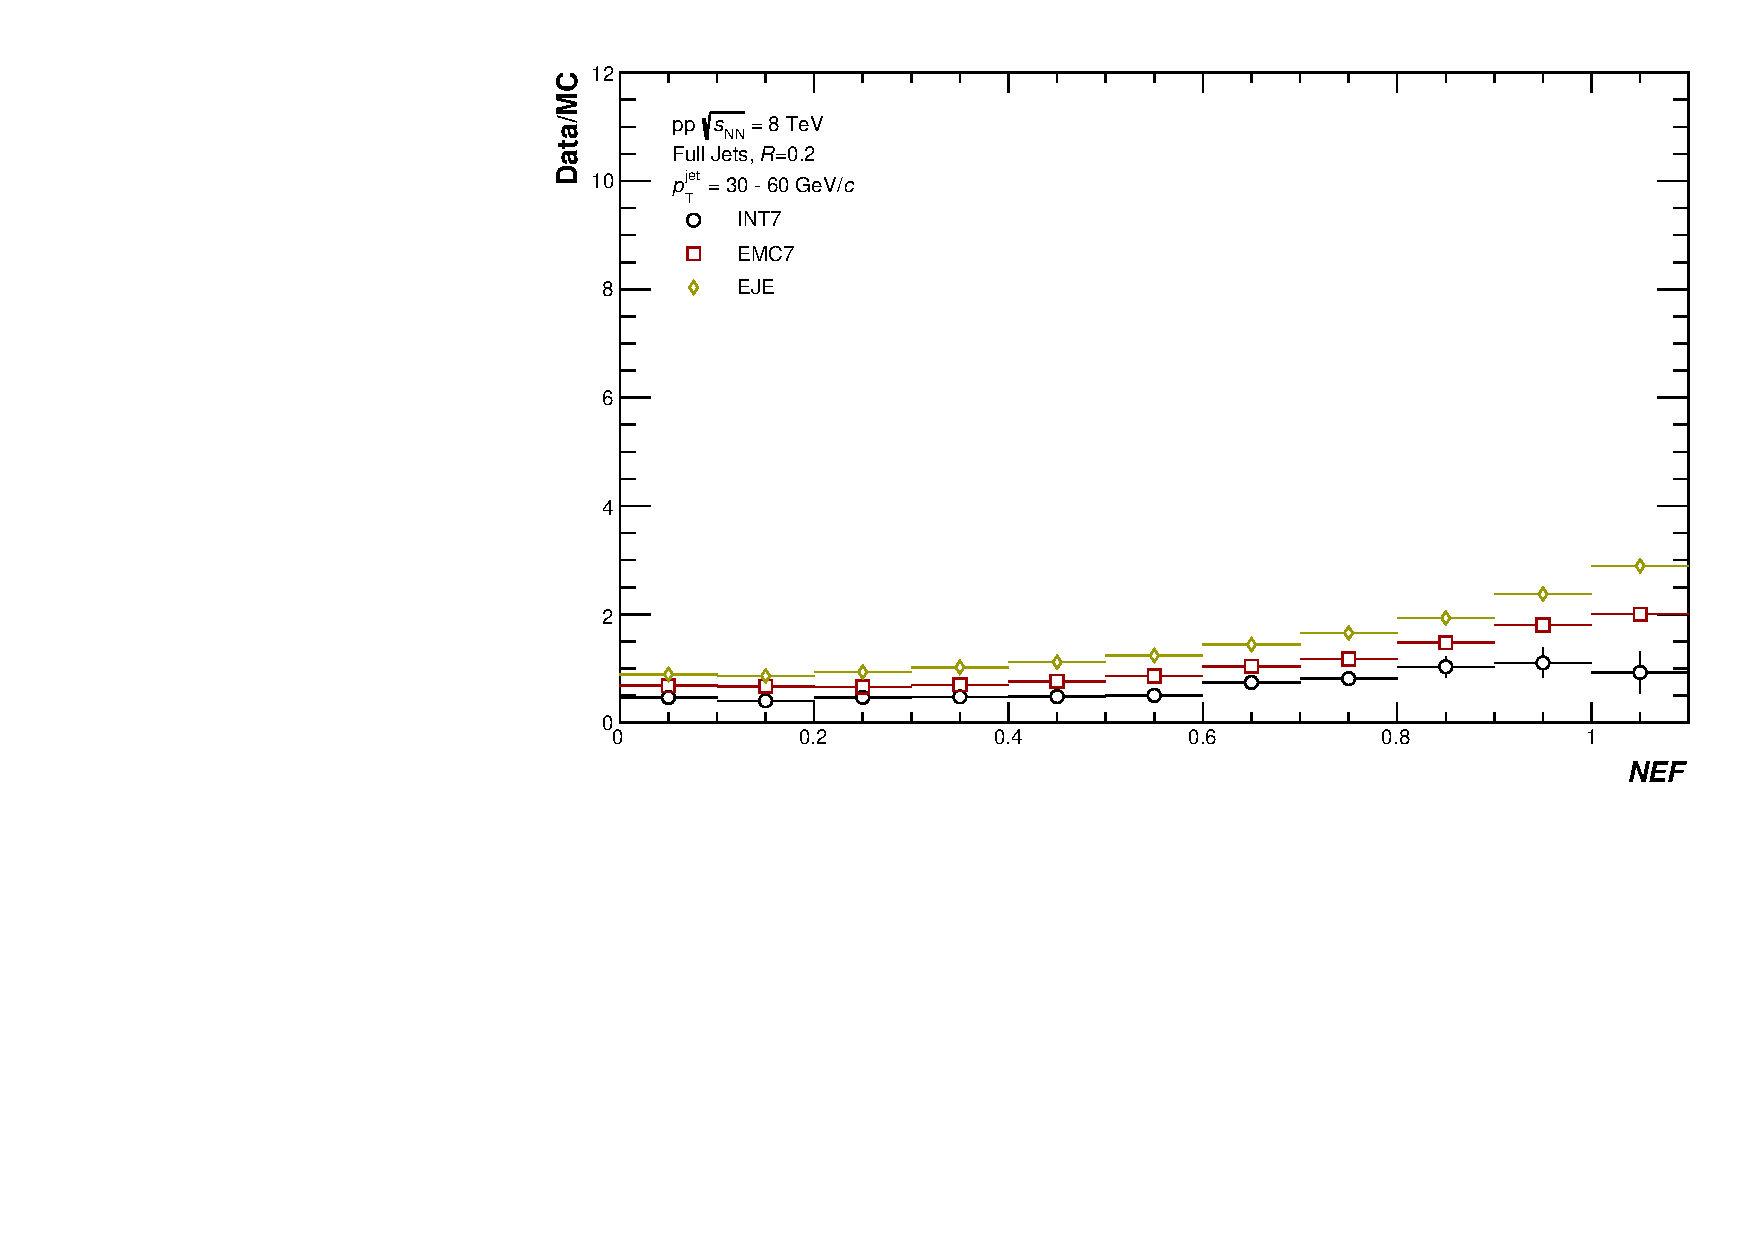
\includegraphics[width=0.49\textwidth]{figures/TriggerBias/NEF/hNEF_ptBin2_R02.pdf}
        \vfill\null
        \columnbreak
            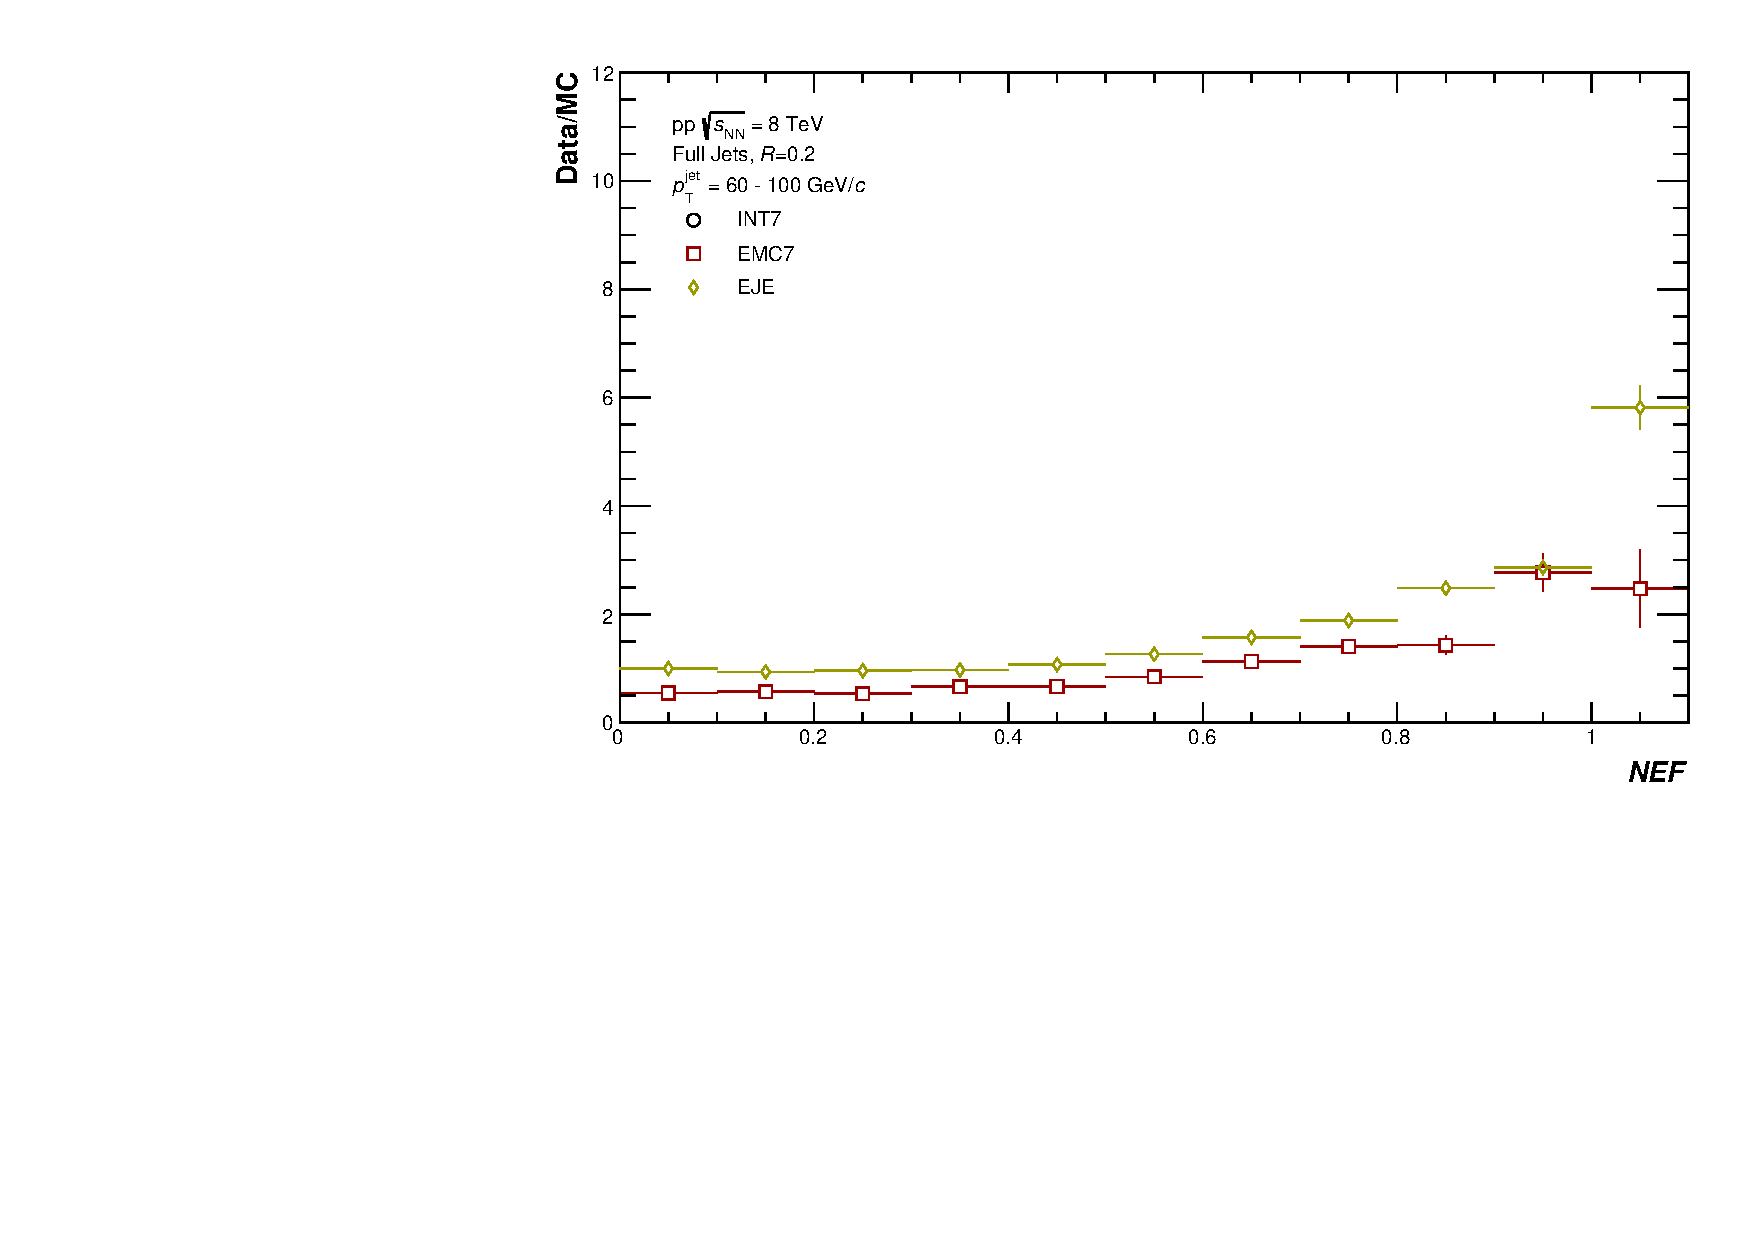
\includegraphics[width=0.49\textwidth]{figures/TriggerBias/NEF/hNEF_ptBin3_R02.pdf}
            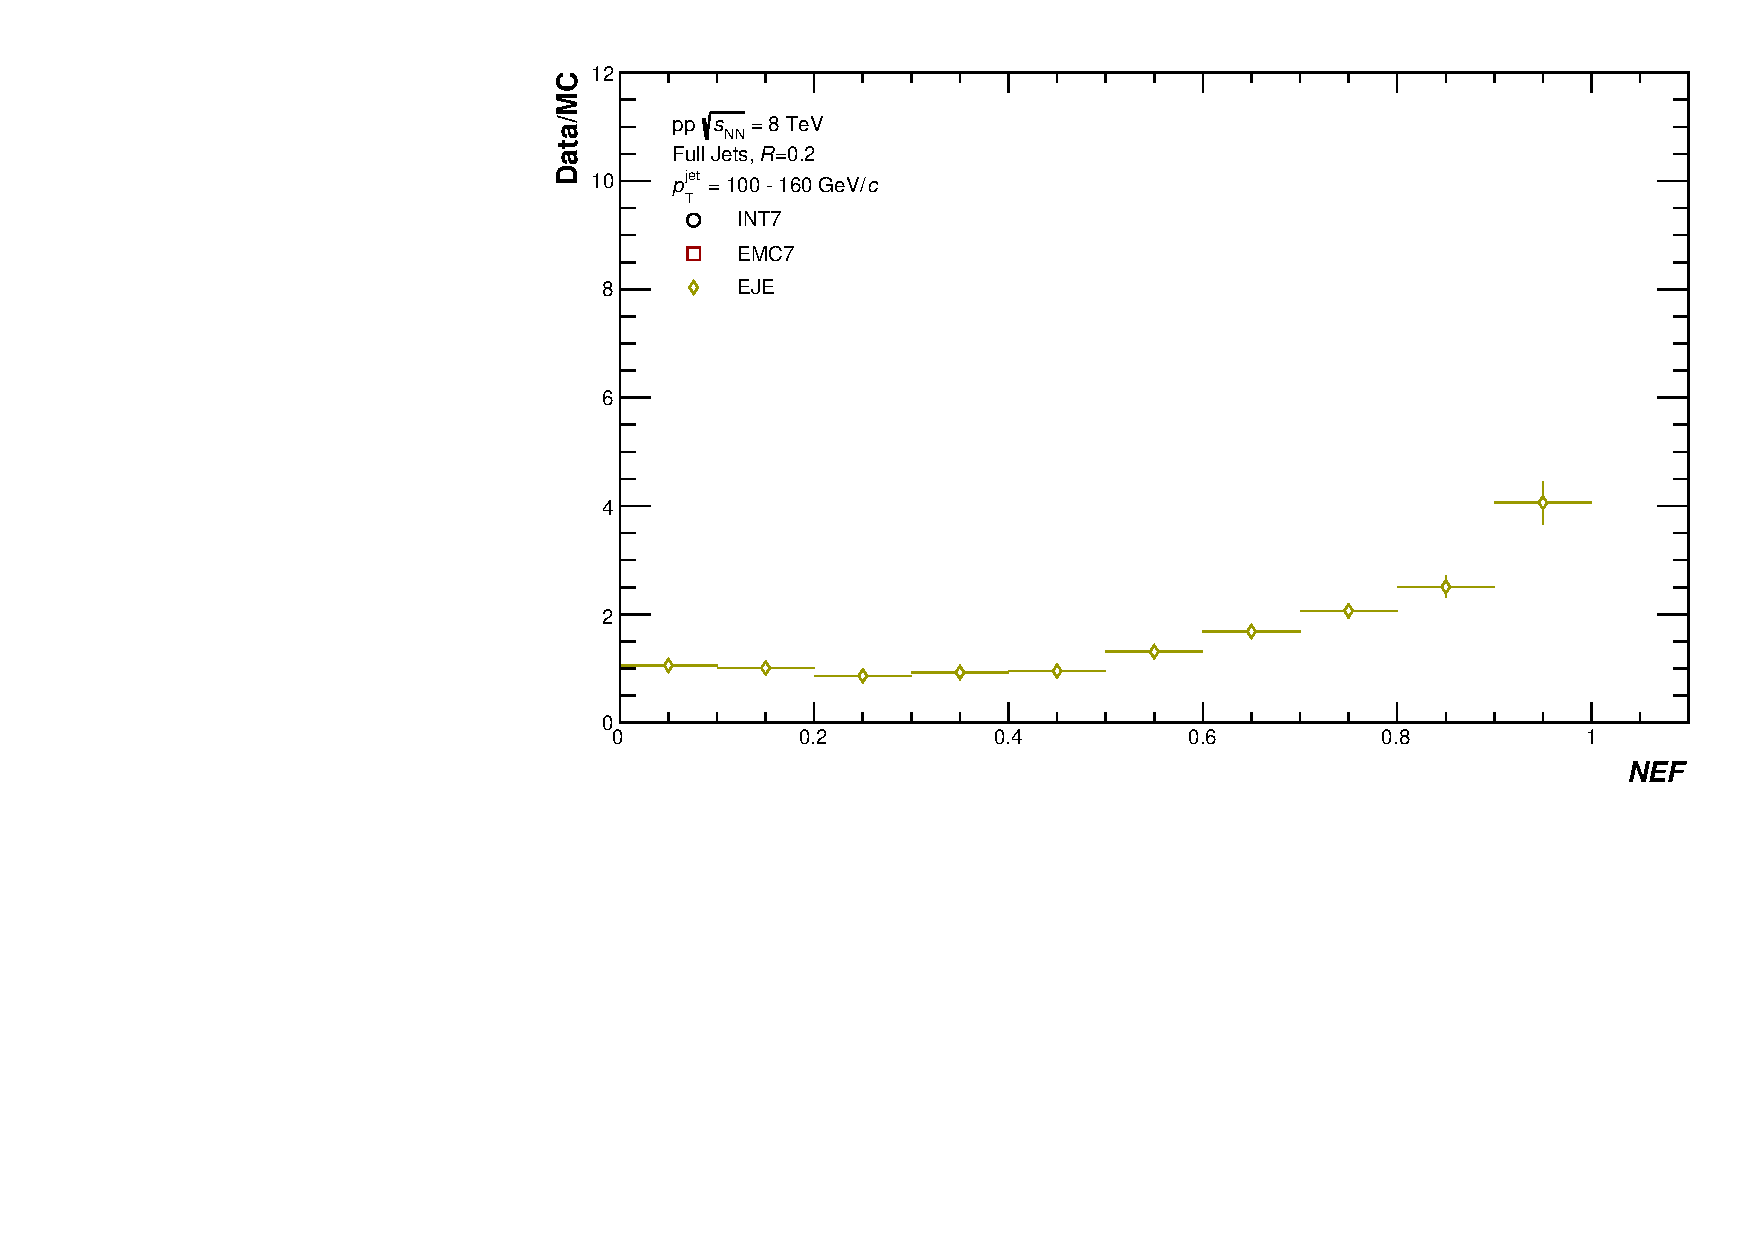
\includegraphics[width=0.49\textwidth]{figures/TriggerBias/NEF/hNEF_ptBin4_R02.pdf}
        \vfill\null
    \end{multicols}
    \caption{neutral energy fraction ratios of \pp data to Monte Carlo for different bins in jet \pT and a jet resolution parameter of R=0.2.}
    \label{fig:TriggerBiasNEFR02}
\end{figure}

\begin{figure}[hbt!]
    \centering
    \begin{multicols}{2}
            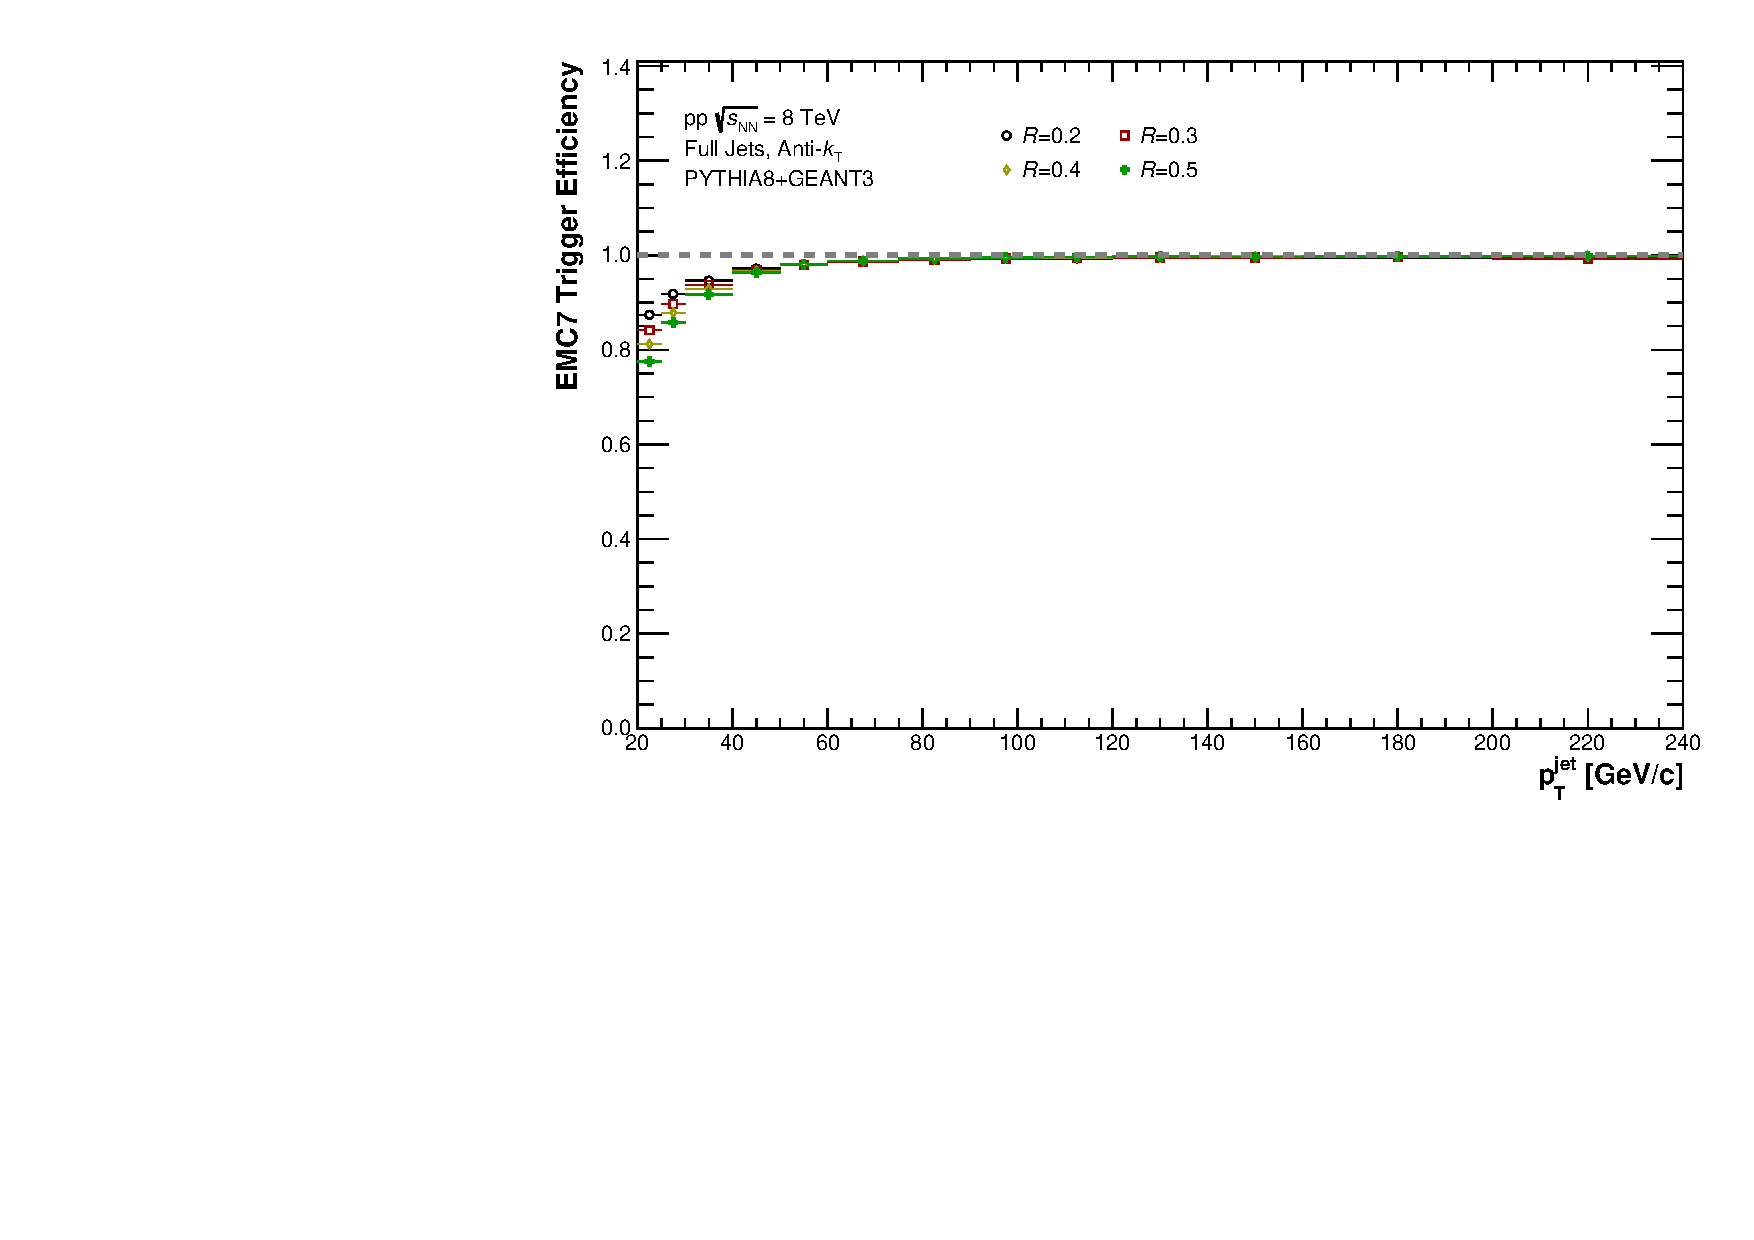
\includegraphics[width=0.49\textwidth]{figures/TriggerEfficiency/hEfficiency_EMC7.pdf}
        \vfill\null
        \columnbreak
            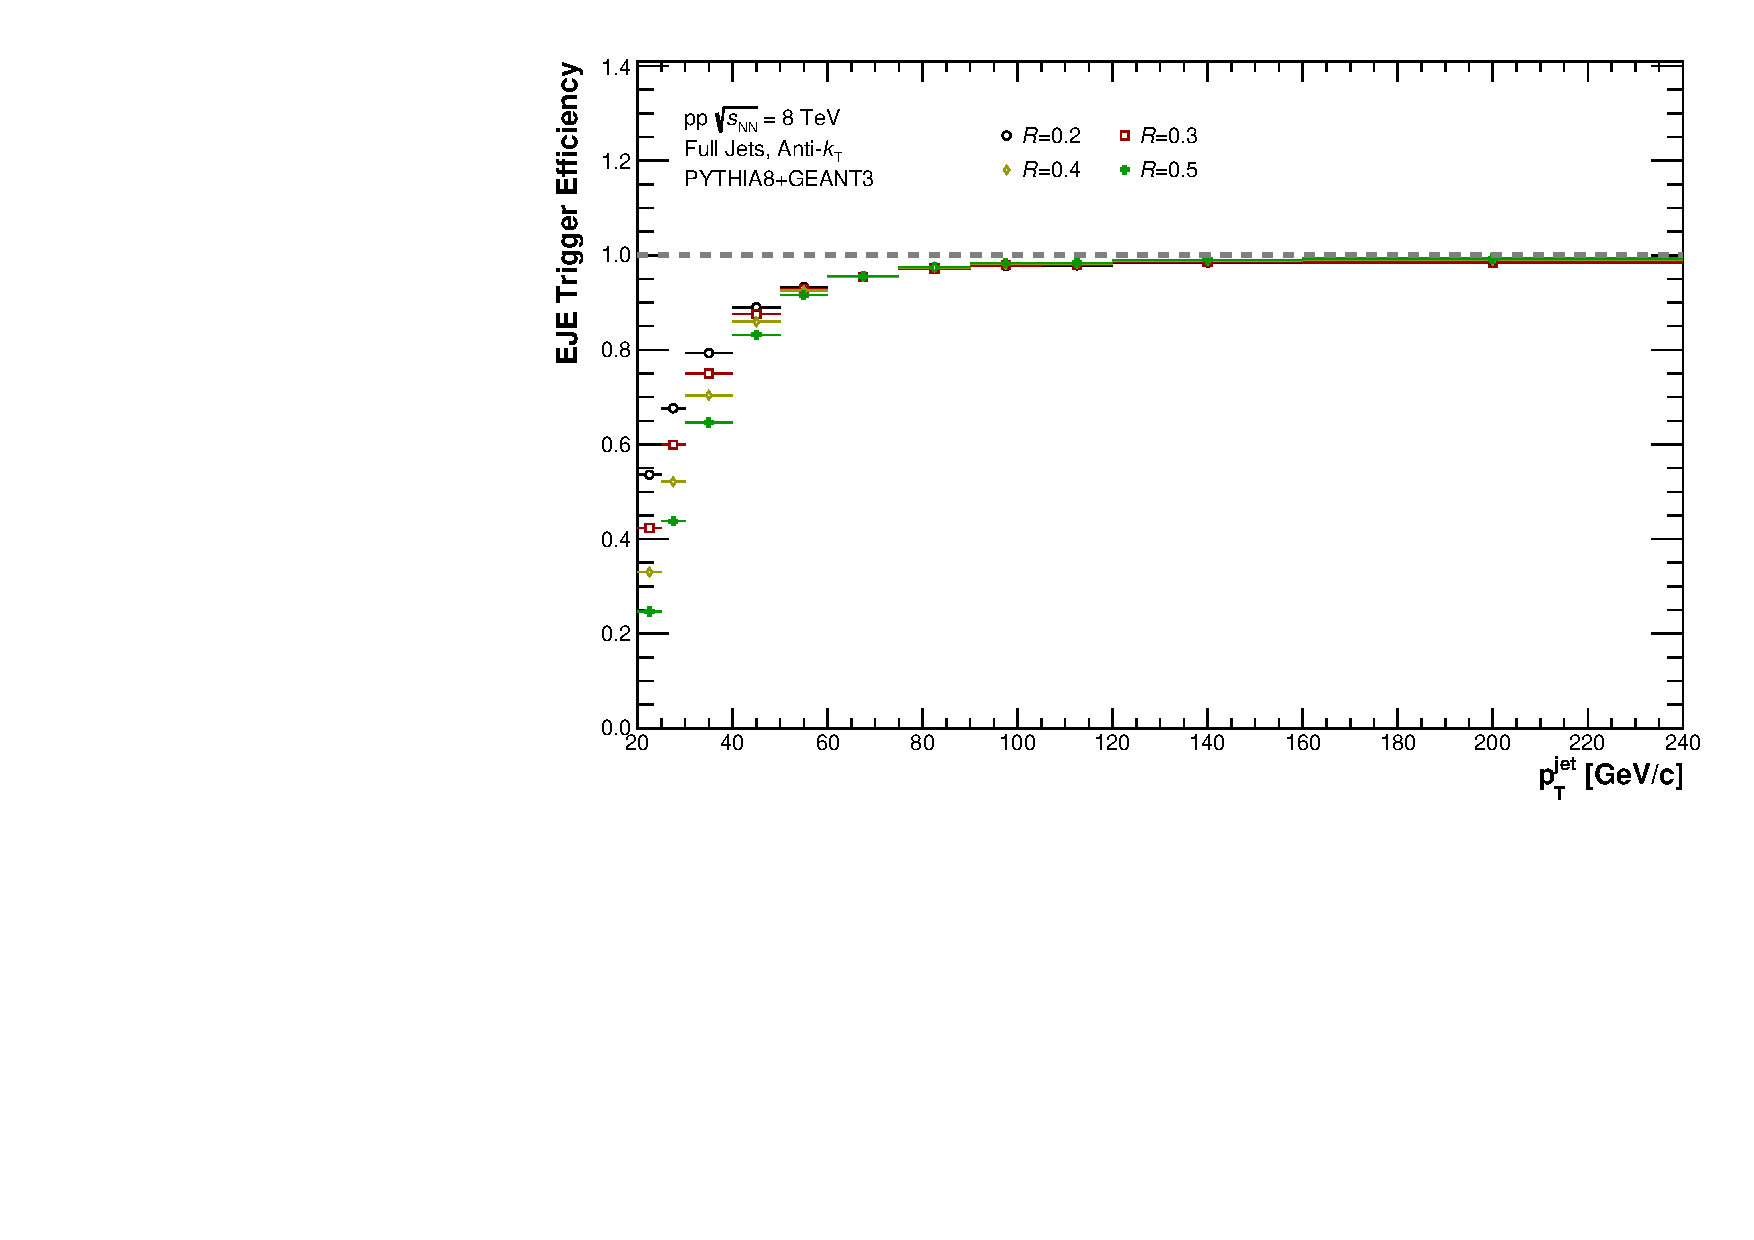
\includegraphics[width=0.49\textwidth]{figures/TriggerEfficiency/hEfficiency_EJE.pdf}
        \vfill\null
    \end{multicols}
    \caption{Trigger efficiency for the EMC7 trigger (left) and the EJE trigger (right), found by taking the ratio of trigger/minimum bias in \pp simulation.}
    \label{fig:TriggerEfficiency_pp}
\end{figure}

\begin{figure}[hbt!]
    \centering
    \begin{multicols}{2}
            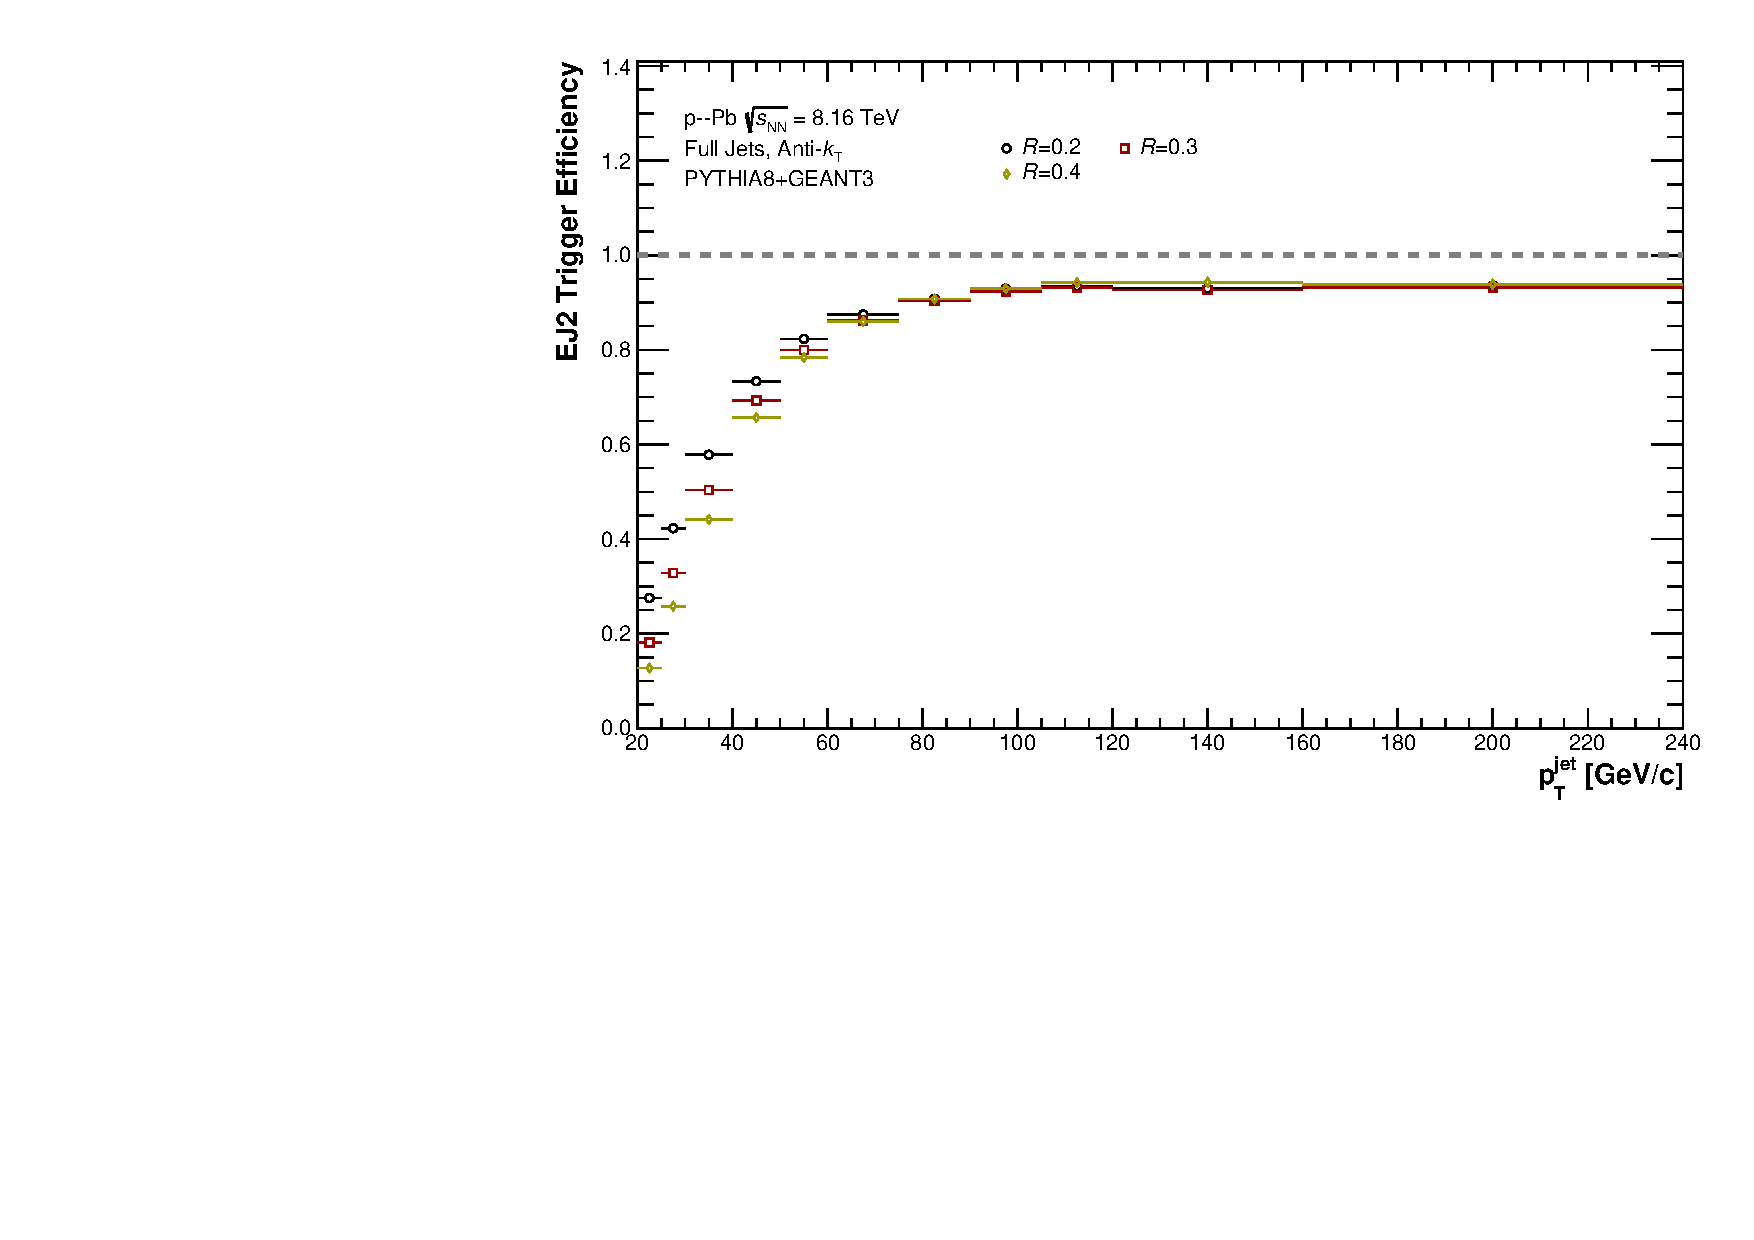
\includegraphics[width=0.49\textwidth]{figures/pPbFigures/TriggerEfficiency/hEfficiency_EJ2.pdf}
        \vfill\null
        \columnbreak
            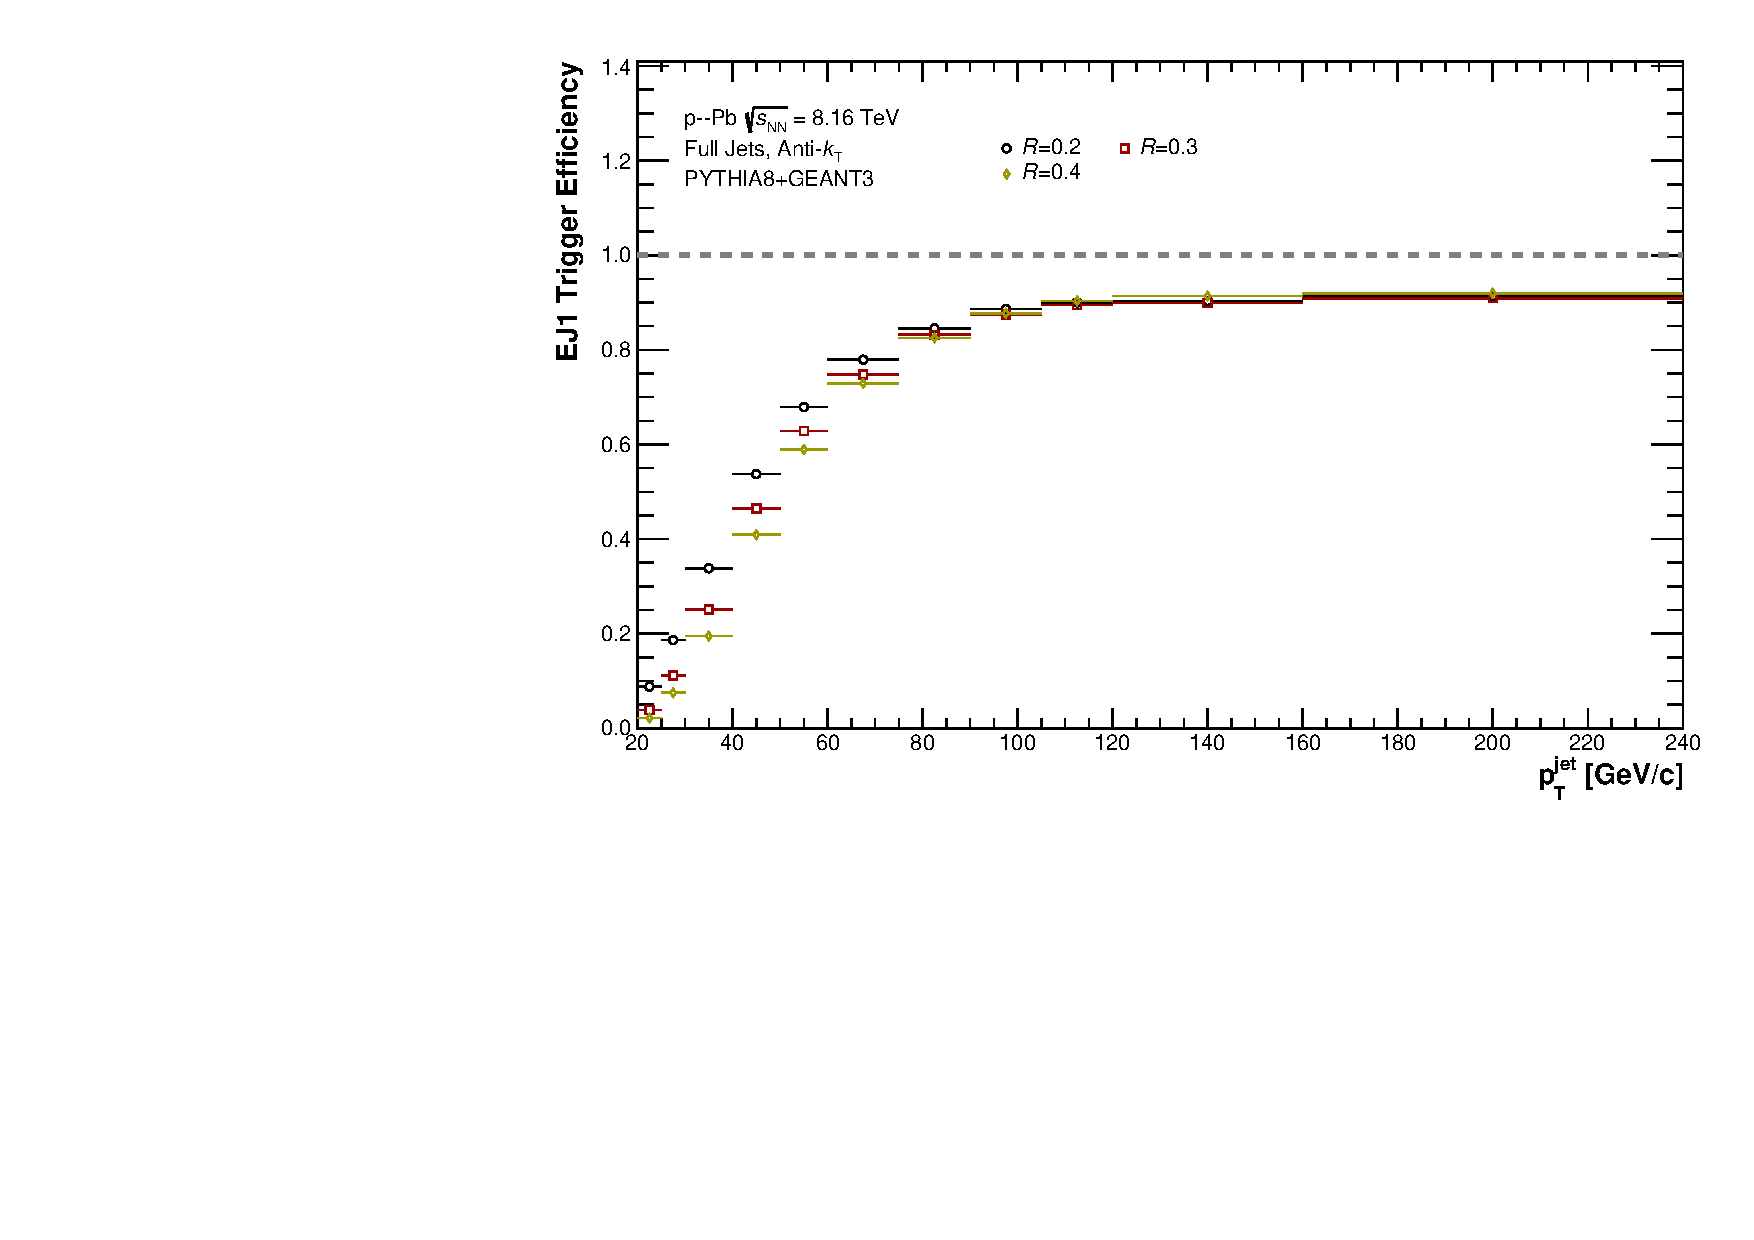
\includegraphics[width=0.49\textwidth]{figures/pPbFigures/TriggerEfficiency/hEfficiency_EJ1.pdf}
        \vfill\null
    \end{multicols}
    \caption{Trigger efficiency for the EJ2 trigger (left) and the EJ1 trigger (right), found by taking the ratio of trigger/minimum bias in \pPb simulation.}
    \label{fig:TriggerEfficiency_pPb}
\end{figure}
\section{Corrections to the Jet Spectra}
\label{ch:Corrections}

The scaling of the jet spectra before unfolding is expressed as

\begin{equation}
    \frac{\mathrm{d}\sigma}{\mathrm{d}p_\mathrm{T} \mathrm{d}\eta} = \frac{1}{L} \frac{\epsilon_\mathrm{vtx}}{A\cdot\epsilon_\mathrm{trg}}\frac{\mathrm{d}N_\mathrm{jet}}{\mathrm{d}p_\mathrm{T} \mathrm{d}\eta} = \frac{\sigma_\mathrm{V0AND}}{N_\mathrm{trg,INT7}\cdot RF} \frac{\epsilon_\mathrm{vtx}}{A\cdot\epsilon_\mathrm{trg}}\frac{\mathrm{d}N_\mathrm{jet}}{\mathrm{d}p_\mathrm{T} \mathrm{d}\eta}
    \label{eq:corrraweq}
\end{equation}    

\noindent
with the corrected trigger yield N$_\mathrm{trg,INT7}$, the vertex finding efficiency $\epsilon_\mathrm{vtx}$, the trigger efficiency $\epsilon_\mathrm{trg}$, and the rejection factor (RF), which is 1 for the INT7 trigger. $L$ is the luminosity of the sample, and A is the acceptance correction. The following sections will discuss these corrections in more detail.

\subsection{Trigger Combination}
\label{sec:Trigger Combination}

The jet spectrum from each trigger covers a different region within the full \pT range of the measurement. The three triggers must be scaled appropriately, and when each successive trigger reaches the bias-free threshold, a transition to that trigger is made. 

The trigger cluster yield for all three triggers for jet radius R = 0.2 can be found in \ref{fig:triggerClusters}. The integrated luminosity inspected by the trigger is independent of the probe, therefore it is sufficient to study only one jet radius. From this, it can be seen that the yields do not overlap. This is due to the downscaling of the minimum bias, EMC7, and EJ2 triggers (to different degrees) in order to allow trigger time for the EMCal triggers to record rare events (jets, in this case).

\begin{figure}
    \centering
    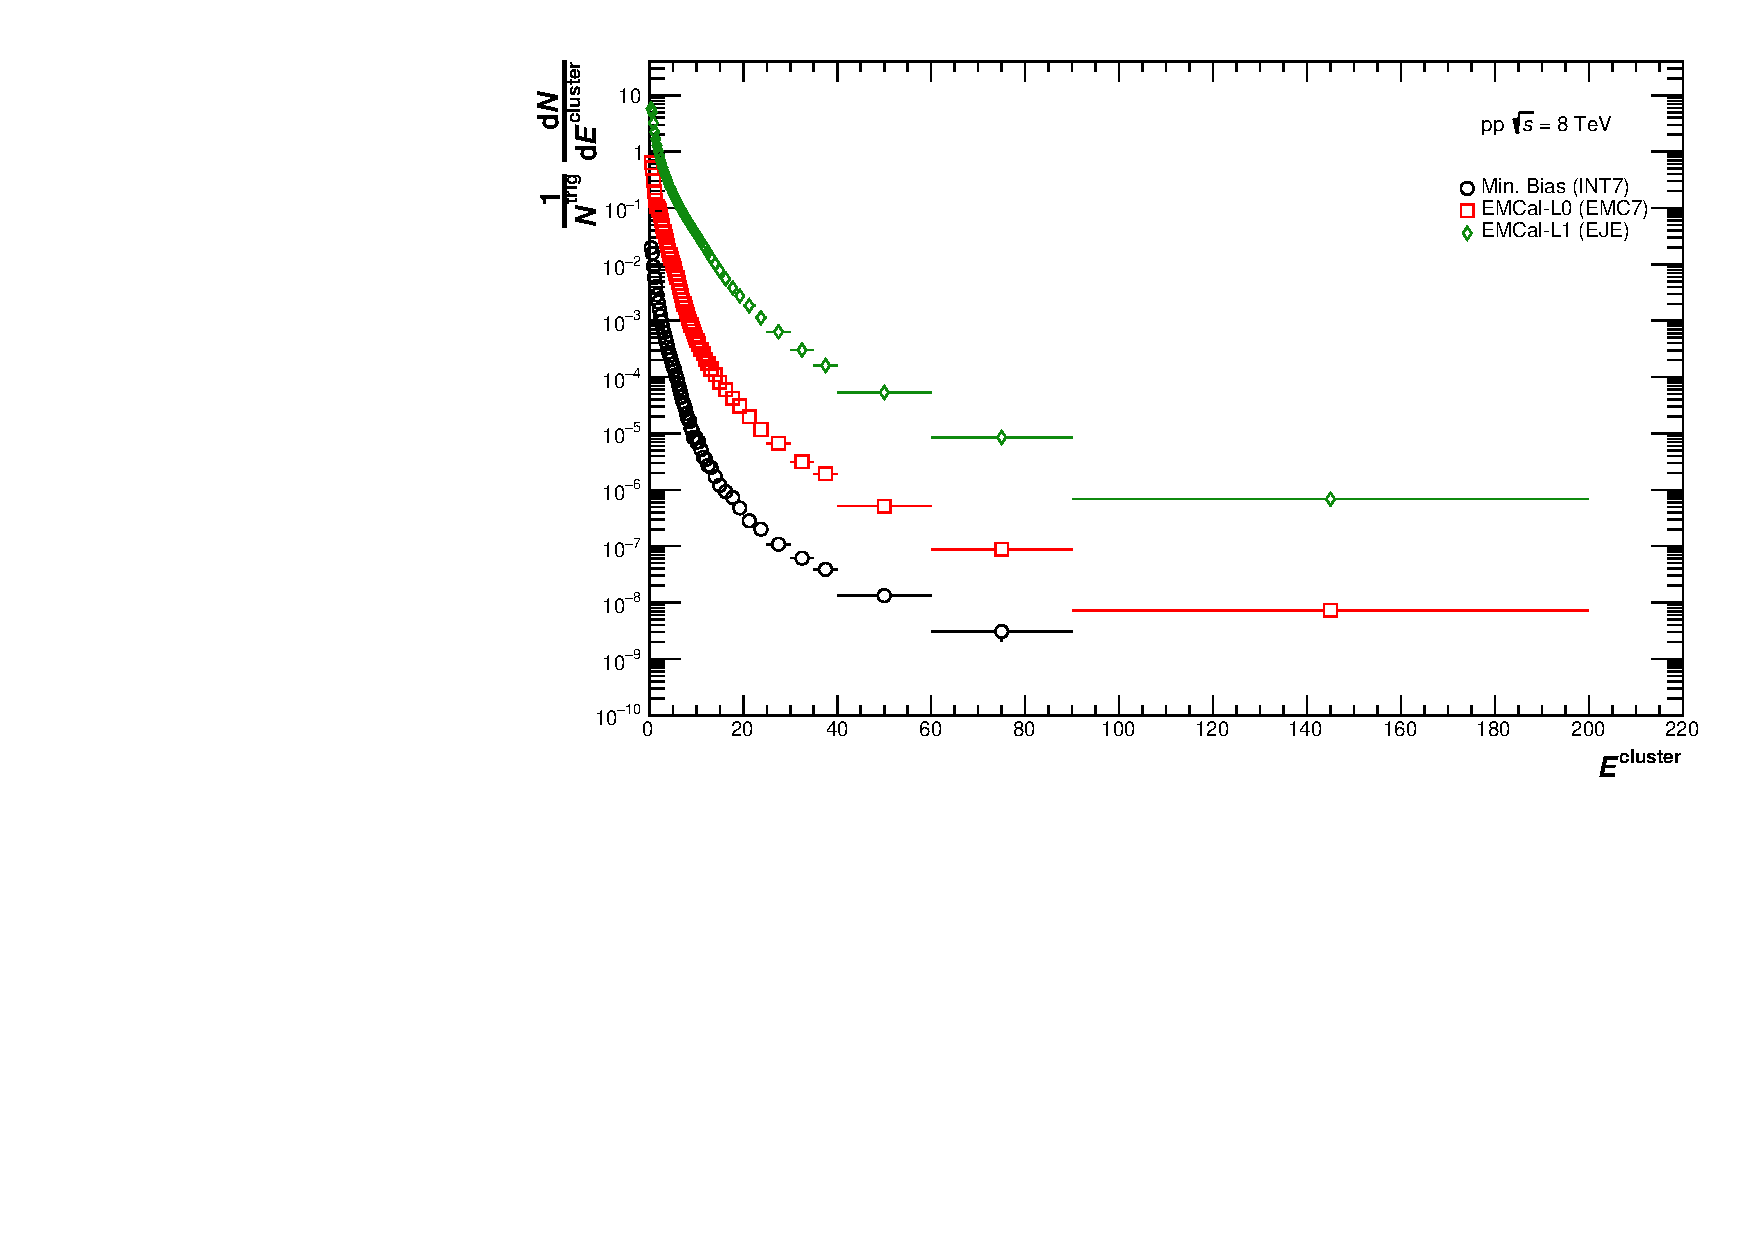
\includegraphics[width=15cm]{figures/TriggerClusters/clusters_R02.pdf}
    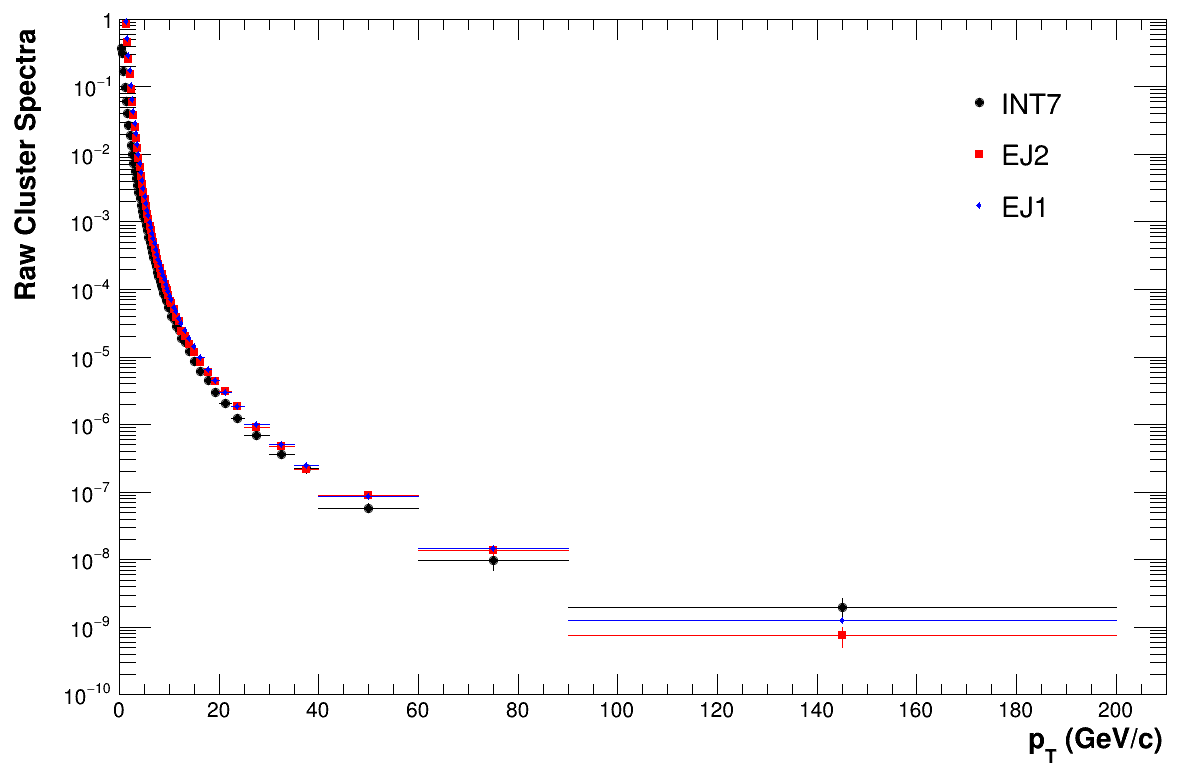
\includegraphics[width=15cm]{figures/pPbFigures/TriggerClusters/rawclusterspectra_alltriggers_R02.png}
    \caption{Trigger cluster yields for the INT7, EMC7, and EJE triggers in \pp (left), and for INT7, EJ2, and EJ1 triggers in \pPb (right). Scaling is required in order for the spectra to overlap.}
    \label{fig:triggerClusters}
\end{figure}

In the 2012 dataset, the downscale factors for the INT7 and EMC7 triggers were not recorded. For this reason, the triggered data must be corrected by the use of rejection factors. These trigger rejection factors are calculated by taking the ratio of the cluster yield between triggers with neighboring thresholds after correction for the trigger efficiency. In this case, the ratio of the EMC7 to INT7 triggers and the ratio of the EJE to EMC7 triggers are taken. A correction must be made for the trigger efficiency. This is done by taking the ratio of the EMCal trigger to minimum bias cluster yields in Monte Carlo. The ratio of cluster yields for different triggers without correction for the cluster trigger efficiency is shown in figure \ref{fig:RejectionFactorsUnscaled}. The plateaus are fit with an error function, and the flat region of the function is taken as the constant rejection factor. The ratios of the cluster yields for different triggers in data after the trigger efficiency correction are shown in Figure~\ref{fig:RejectionFactors}. The low-\pT region shows the range in which the trigger has not yet reached maximum efficiency and the behavior of the cluster spectra is not described by the Monte Carlo. The measurement is reliable at momenta in the region where the ratios reach a plateau. These plateaus are fit with a constant to find the rejection factor and its associated uncertainty. The jet spectrum for the EMC7 trigger is then divided by the rejection factor derived from the EMC7 to INT7 trigger cluster ratio, while the jet spectrum for the EJE trigger is divided by both rejection factors.

\begin{figure}
    \centering
    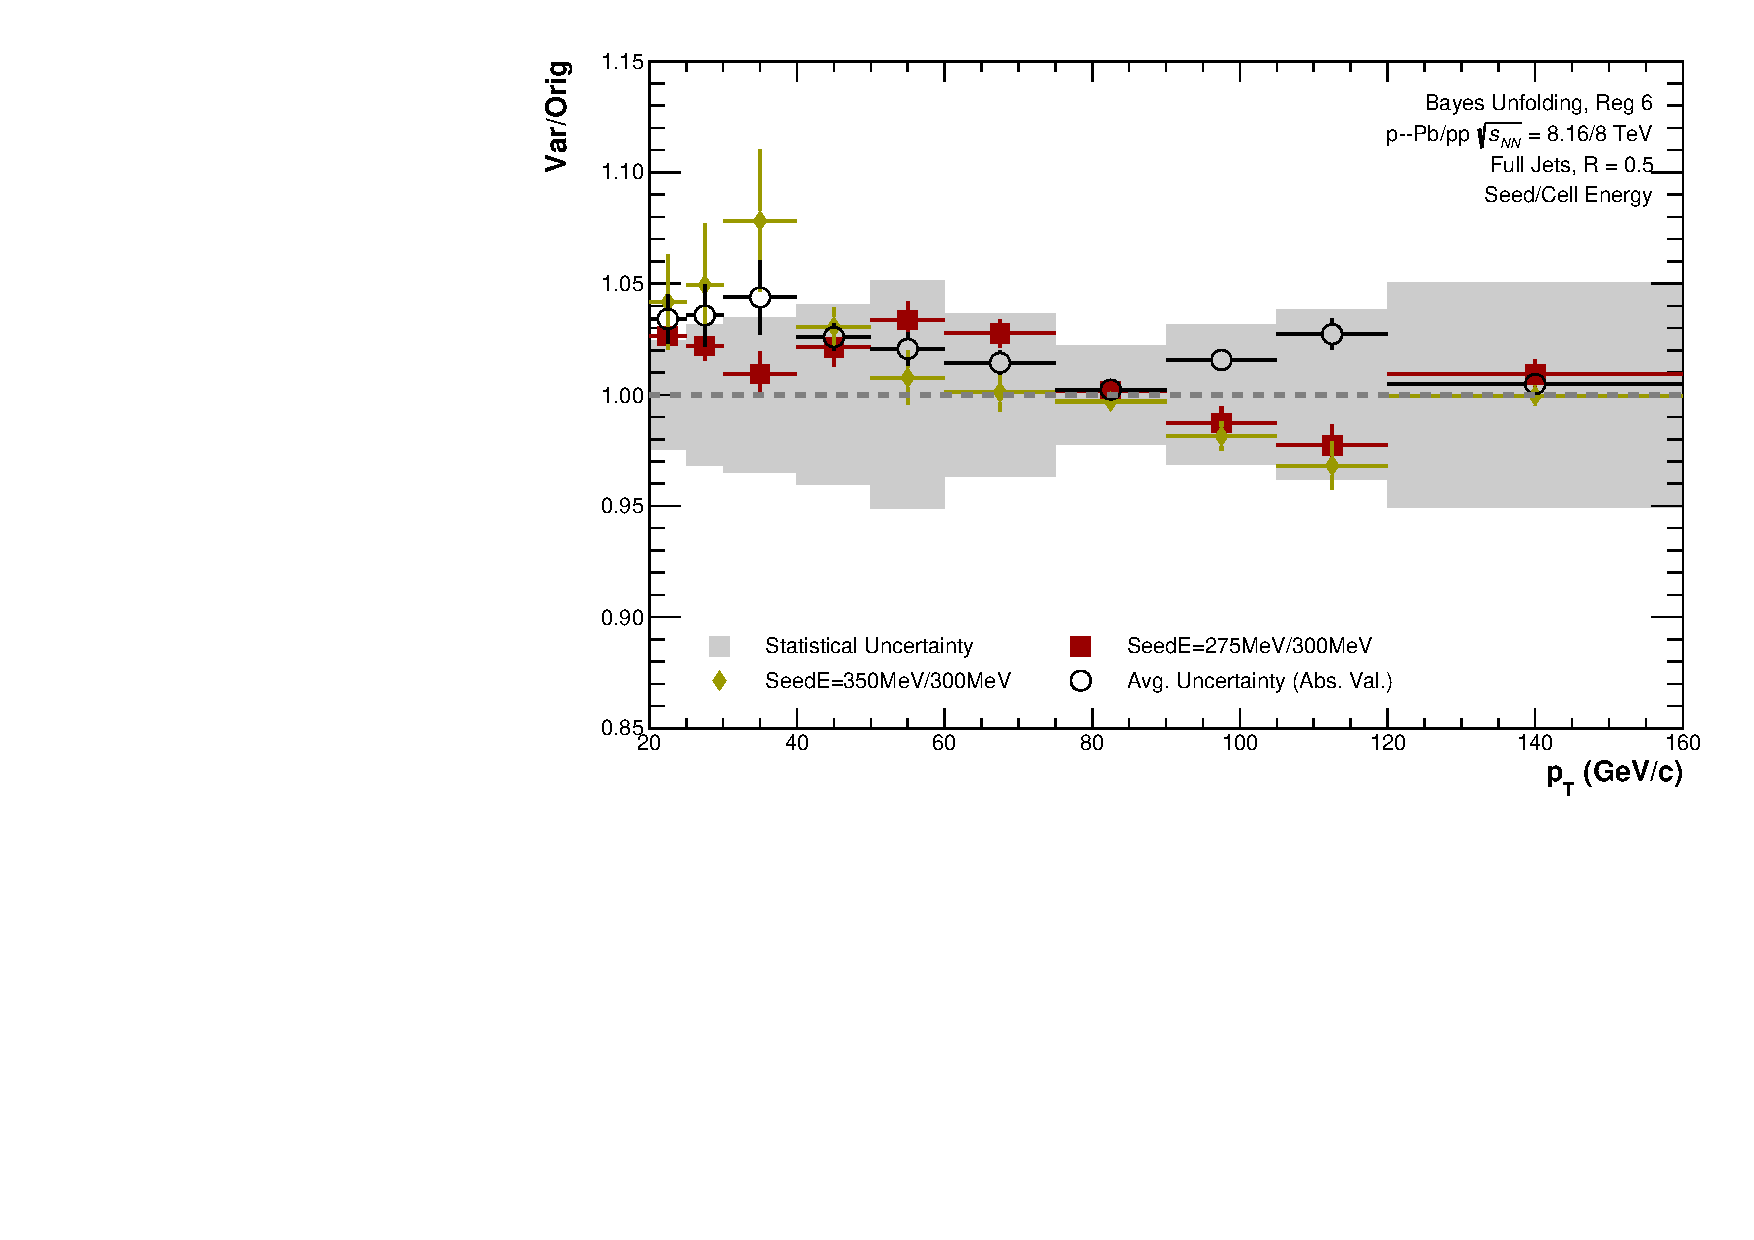
\includegraphics[width=15cm]{figures/RejectionFactors/RF_R02_Unscaled_Default.pdf}
    \caption{Rejection factors for the EMC7 trigger and the EJE trigger, found by taking the ratio of the event-normalized trigger yields of the EMC7/INT7 triggers and EJE/EMC7 triggers, respectively.}
    \label{fig:RejectionFactorsUnscaled}
\end{figure}


\begin{figure}[hbt!]
    \centering
    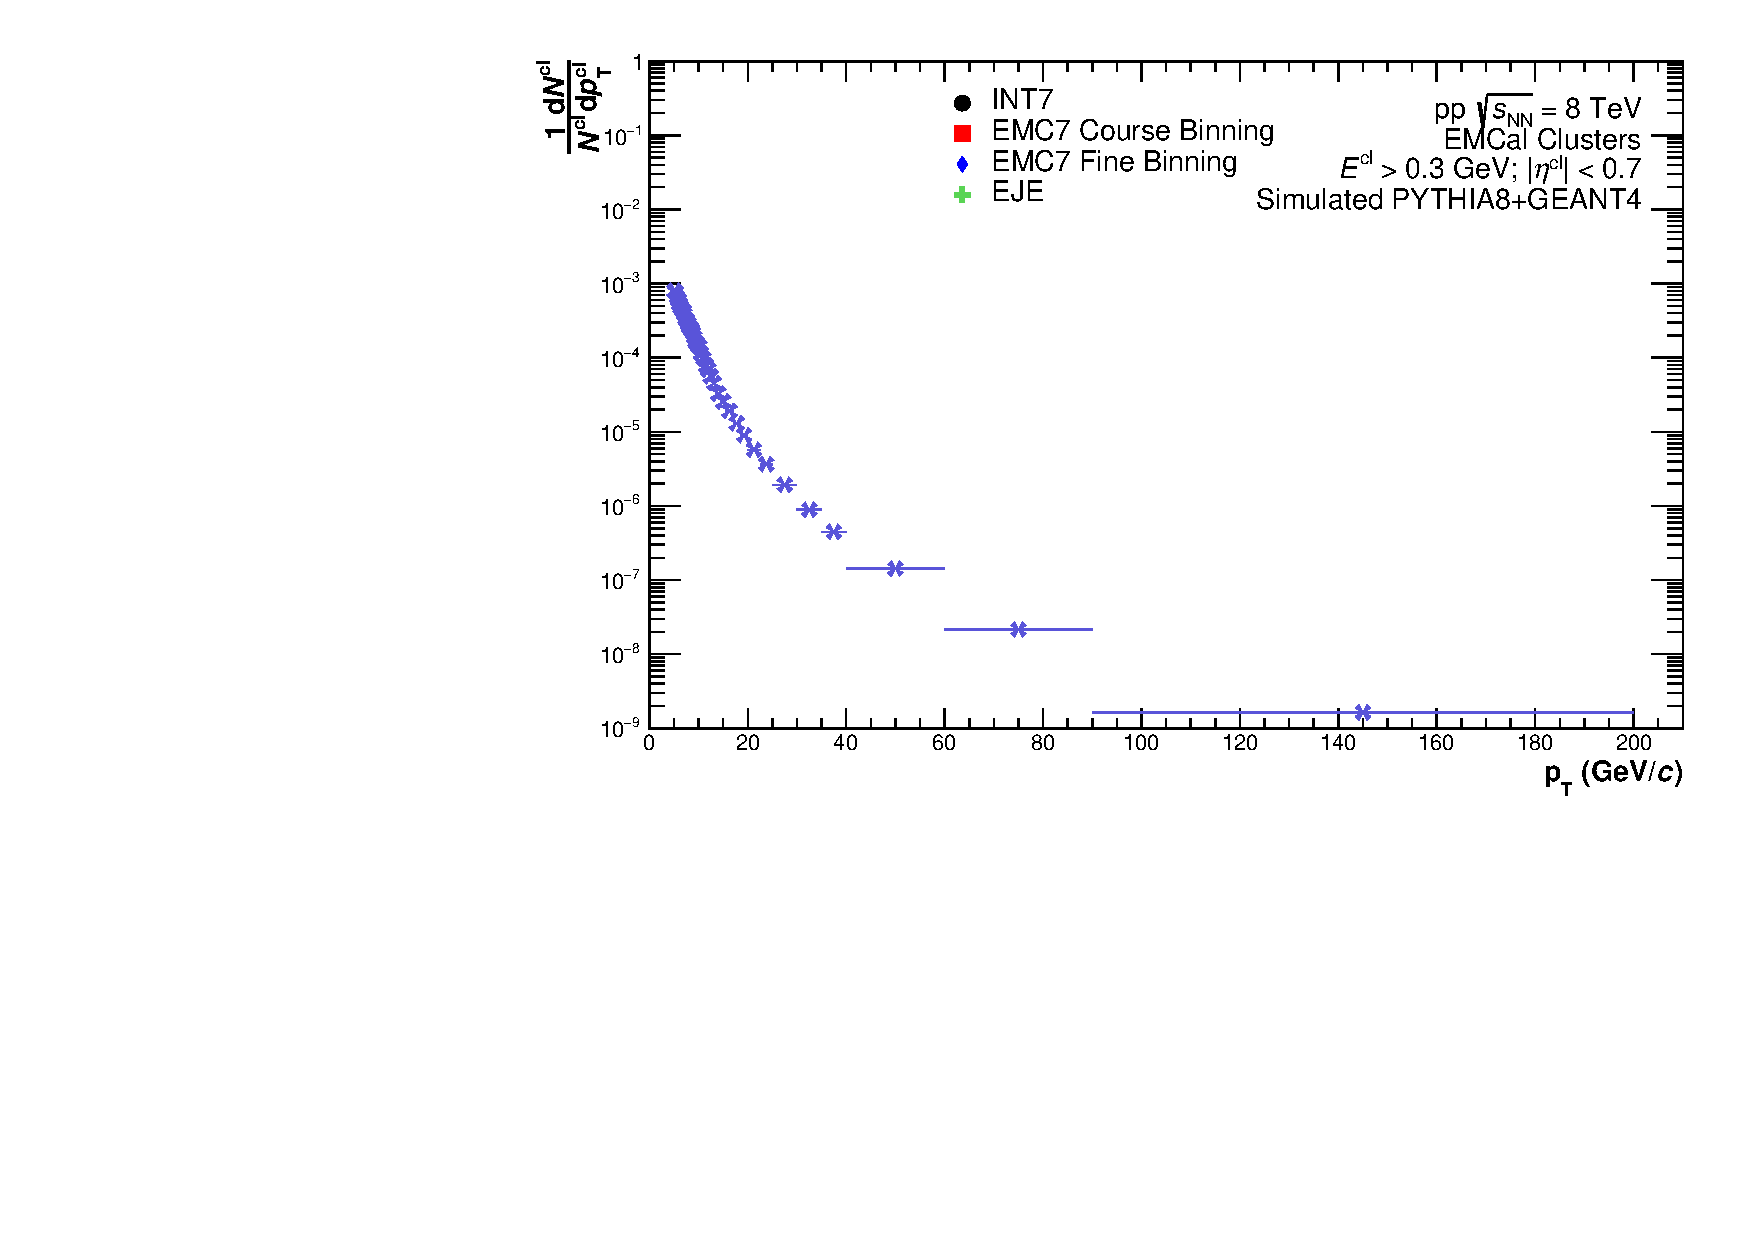
\includegraphics[width=15cm]{figures/RejectionFactors/RF_R02_Default.pdf}
    \caption{Rejection factors in \pp collisions for the EMC7 trigger and the EJE trigger. The ratio is taken of the event-normalized trigger yields of the EMC7/INT7 triggers and EJE/EMC7 triggers and scaled by the cluster trigger efficiency. The plateau is fit with a constant to find the rejection factor.}
    \label{fig:RejectionFactors}
\end{figure}

In the \pPb dataset, the observed integrated luminosity can be used to scale the spectra in place of the rejection factors. The detector readout speed is determined by the slowest detector in the trigger cluster. If that detector is removed from the cluster, more collisions can be recorded. If more than one trigger cluster is used in the analysis, the effective live time can be different. As there is typically at least one trigger shared by two clusters, this shared trigger can be used to compare the clusters and find the required scale corrections. Because the corrections factorize, the integrated luminosity of the trigger can be calculated based on the event count and the downscaling of the minimum bias trigger. In the \pp dataset, no overlap existed between the clusters, so the rejection factors were used instead.


\begin{figure}[hbt!]
    \centering
    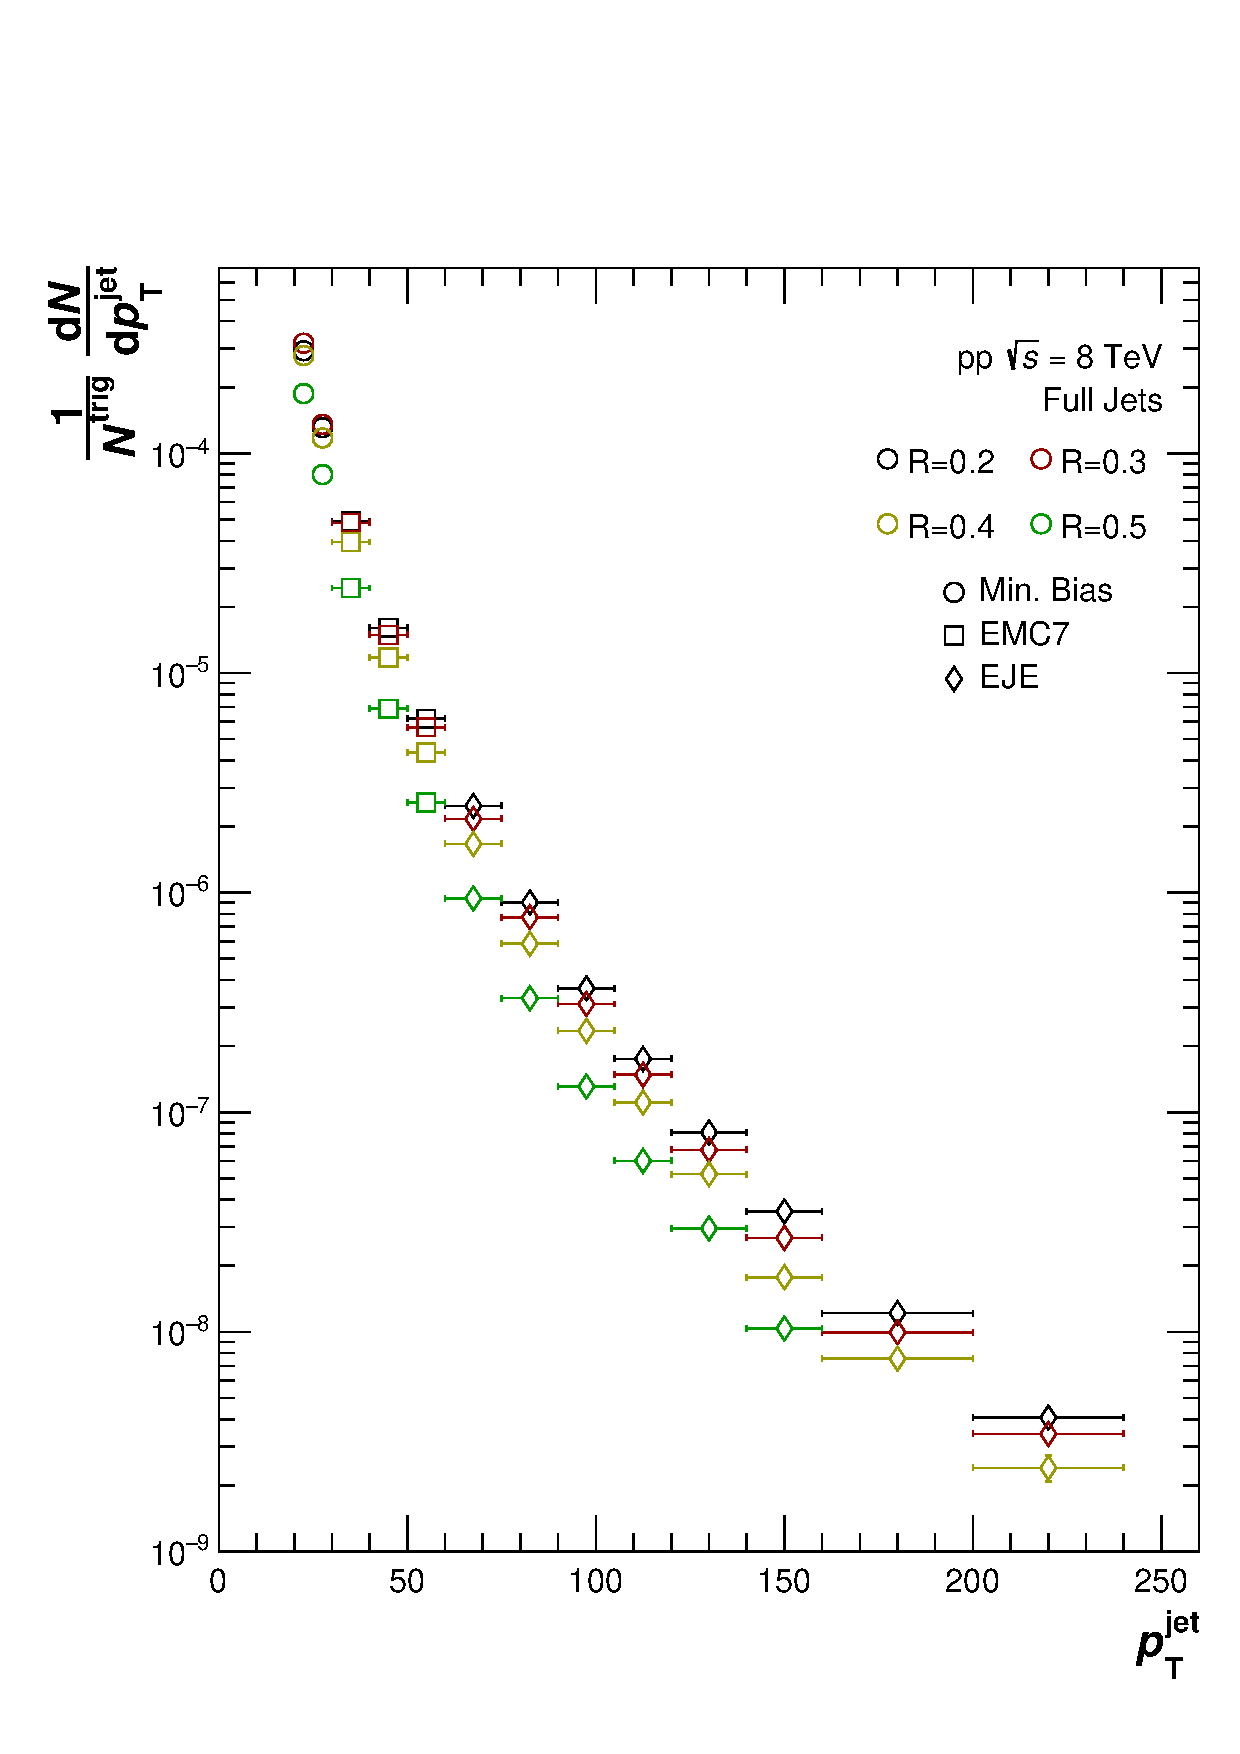
\includegraphics[width=0.49\textwidth]{figures/CorrRawSpec/corrRawSpec.pdf}
    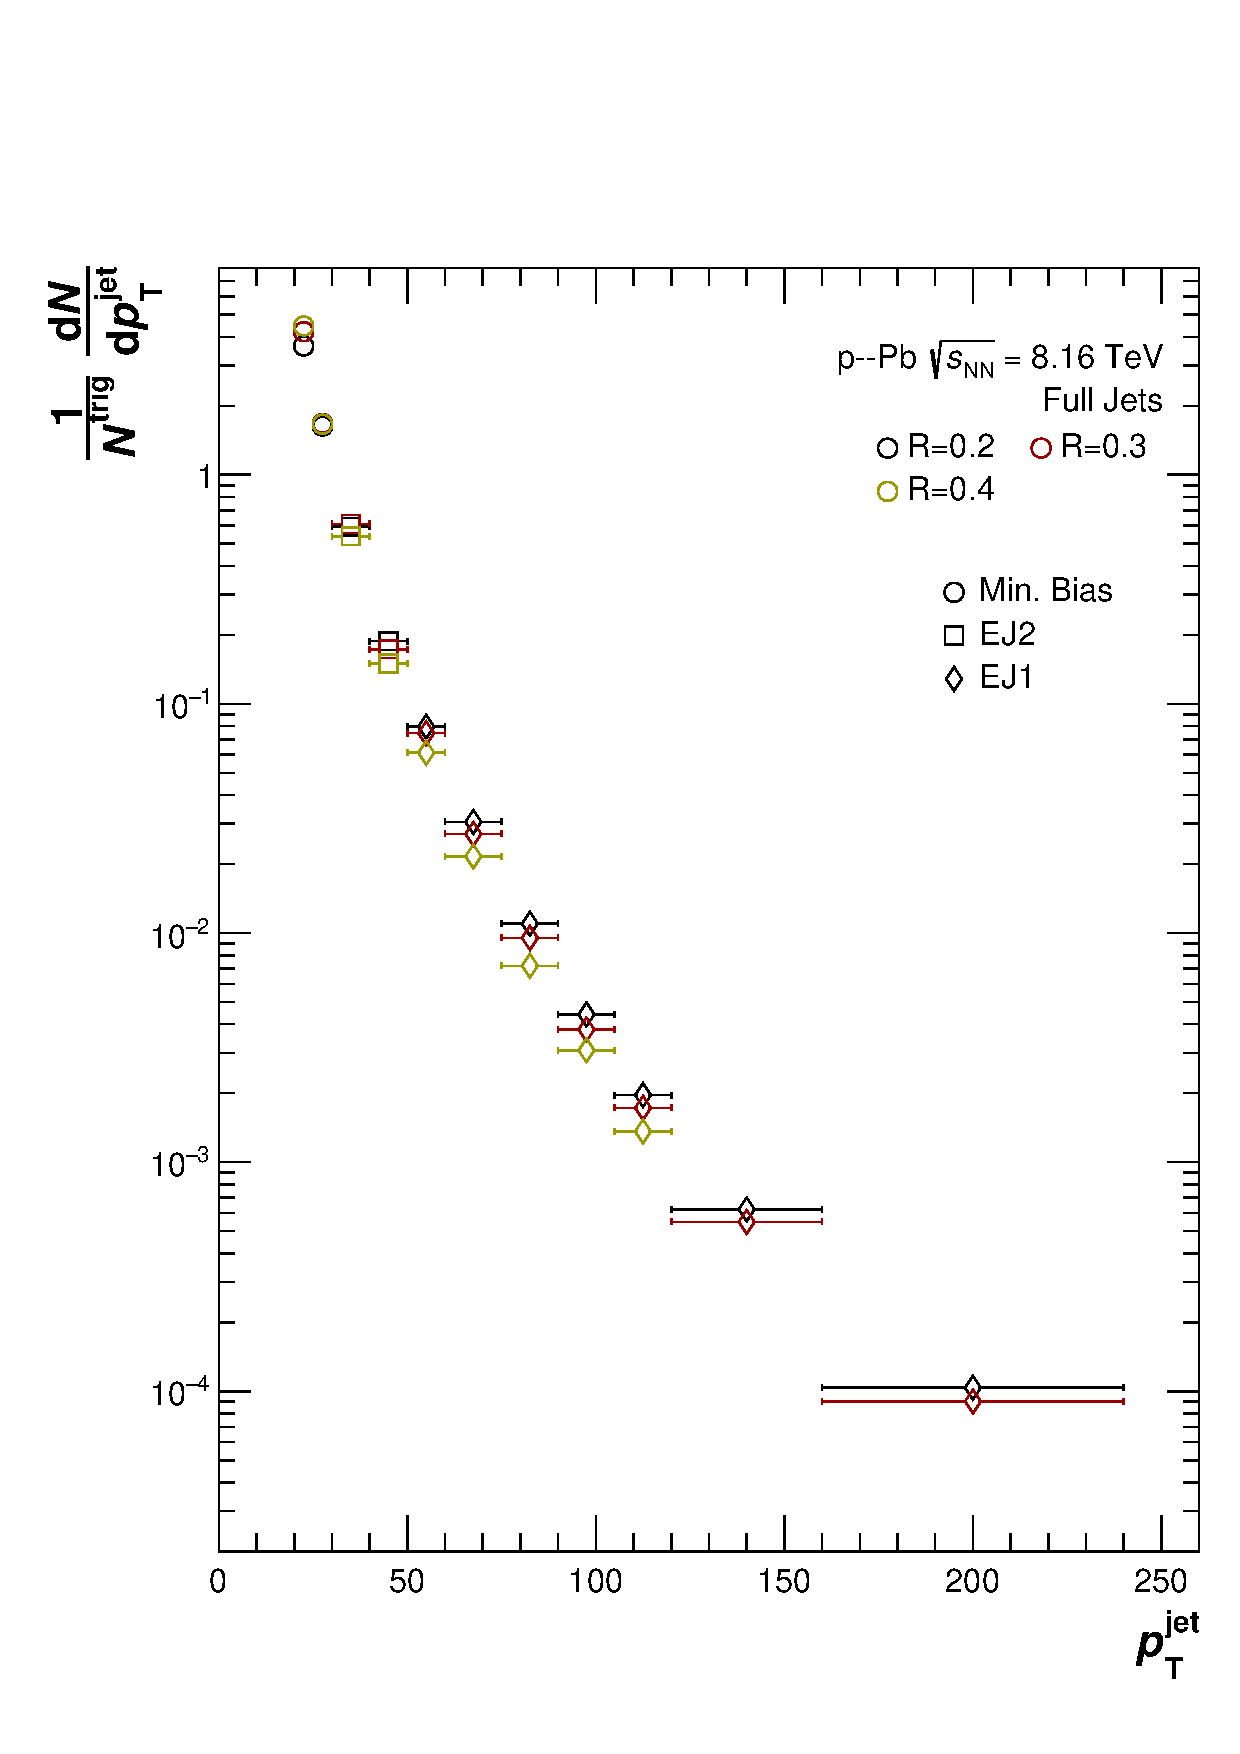
\includegraphics[width=0.49\textwidth]{figures/pPbFigures/CorrRawSpec/corrRawSpec.pdf}
    \caption{Jet spectra in \pp (left) and \pPb (right) collisions for the three triggers after corrections for various jet radii.}
    \label{fig:CorrRawSpec}
\end{figure}

The full spectrum before unfolding is constructed by combining the spectra from the three trigger classes after the application of the scaling factors. Figure~\ref{fig:CorrRawSpec} shows the comparison of the spectra from the three triggers in \pp for jets with different jet radii. 

\subsection{Scaling of the Jet Spectrum}
\label{sec:xsecNomalization}

Since the jet yield was measured only in the EMCal acceptance, a correction for the limited acceptance has to be applied. The acceptance correction is

\begin{equation}
    A = \frac{\Delta\eta \Delta\phi}{2\pi}
\end{equation}

where $\Delta\eta = 1.4 - 2R$ and $\Delta\phi = 1.745 - 2R$ for \pp, and $\Delta\eta = 1.4 - 2R$ and $\Delta\phi = 1.887 - 2R$ for
\pPb. The azimuthal correction is different for the \pPb dataset because extra EMCal modules were added during long shutdown 1, between run 1 and run 2.

The number of events has to be corrected for the vertex finding efficiency. This is done by dividing the spectrum by the efficiency, which is defined as the fraction of events before and after vertex selection and is evaluated before the vertex-z cut. The vertex finding efficiency has been determined from the event counters for accepted and rejected events to be 94.8$\%$ for INT7, 99.2$\%$ for EMC7, and 99.6$\%$ for EJE. EMCal triggered events have a higher multiplicity on average, so more tracks contribute to the vertex reconstruction, especially in pp-collisions. Since luminosity scaling is used in the \pPb dataset instead of the rejection factors, the vertex finding efficiency from the INT7 reference trigger is used for all triggers. In this case, the INT7 vertex finding efficiency is 98.6\%.

\subsection{Background subtraction}
\label{sec:backgroundSubtraction}

In hadronic collisions, reconstructed jets from hard scatterings are not the only particles in the event. Contributions from softer processes will sometimes get clustered together and reconstructed as a jet. Other than in high-multiplicity events, this contribution in \pp collisions is small, but in \pPb collisions, it is large enough that it must be corrected for.

The method used in this analysis to subtract the underlying event was developed by the CMS collaboration for sparse background environments and is termed the $\rho$-sparse method~\cite{CMS:2012rmf}. This method defines the transverse momentum background density as 

\begin{equation}
    \rho_{\text{CMS}} = median\{\frac{{\text{\pT}}_{jet}^{k_T}}{A_{jet}^{k_T}}\} \cdot C
\end{equation}

\noindent
where ${\text{\pT}}_{jet}^{k_T}$ is the transverse momentum of a jet clustered with the $k$\textsubscript{T} algorithm, $A_{jet}^{k_T}$ is the area of that jet, and $C$ is the particle occupancy factor, used to account for regions without any particles. It is defined as

\begin{equation}
    C = \frac{\Sigma_{\text{j}}A_{\text{j}}}{A_{\text{acc}}}
\end{equation}

\noindent
where $A_\text{j}$ is the area of each $k$\textsubscript{T} jet with at least one real track and $A_{\text{acc}}$ is the total particle acceptance. It can be thought of as the covered area divided by the total area, showing how full or empty the event is. The $\rho$ distribution for all three triggers is shown in Figure~\ref{fig:Rho_distribution} for jets with resolution parameter $R$ = 0.2, 0.3, and 0.4. The effect from background is greatest at low momenta and the effect decreases with increasing jet \pT. Since the INT7 trigger covers the low momentum range for this measurement, only the $\rho$ distribution for the INT7 trigger is used for this analysis. For $R$ = 0.2, the distribution is smoothly falling with a maximum at zero. With increasing jet resolution parameter, the distribution becomes more peaked at zero and has a longer tail at high $\rho$ values. This is due to the fact that the highest momentum (signal) jet is excluded from the background calculation, and larger radius jets become increasing difficult to fit inside the acceptance without overlapping with the highest momentum jet. For this reason, and because the background distribution is calculated per unit area, the calculation of $\rho$ at a $k$\textsubscript{T} jet resolution parameter of $R$ = 0.2 is used for all jet radii.

A possible alternative to this method bypasses the limitation of the EMCal acceptance~\cite{anaNoteMConnors}. Instead of calculating the background from a cone within the EMCal acceptance, the entire TPC acceptance is used to calculate the background. A scaling factor is then applied to $\rho$, defined as 

\begin{equation}
    S = \frac{E_{\text{EMC}}+\text{\pT}_\text{EMC}}{\text{\pT}_\text{TPC}}\frac{A_{\text{TPC}}}{A_{\text{EMC}}}
\end{equation}

\noindent
The first term is the ratio of the sum of the total energy from clusters in the EMCal after the hadronic correction is applied and the total momentum of all charged track pointing towards the EMCal acceptance to the total momentum of all charged tracks within the TPC acceptance. The second term is a normalization factor for the relative acceptances of the TPC and EMCal. As an extension of this thesis, this background subtraction technique will be applied to the \pPb data in order to compare these methods.


\begin{figure}[hbt!]
  \centering
  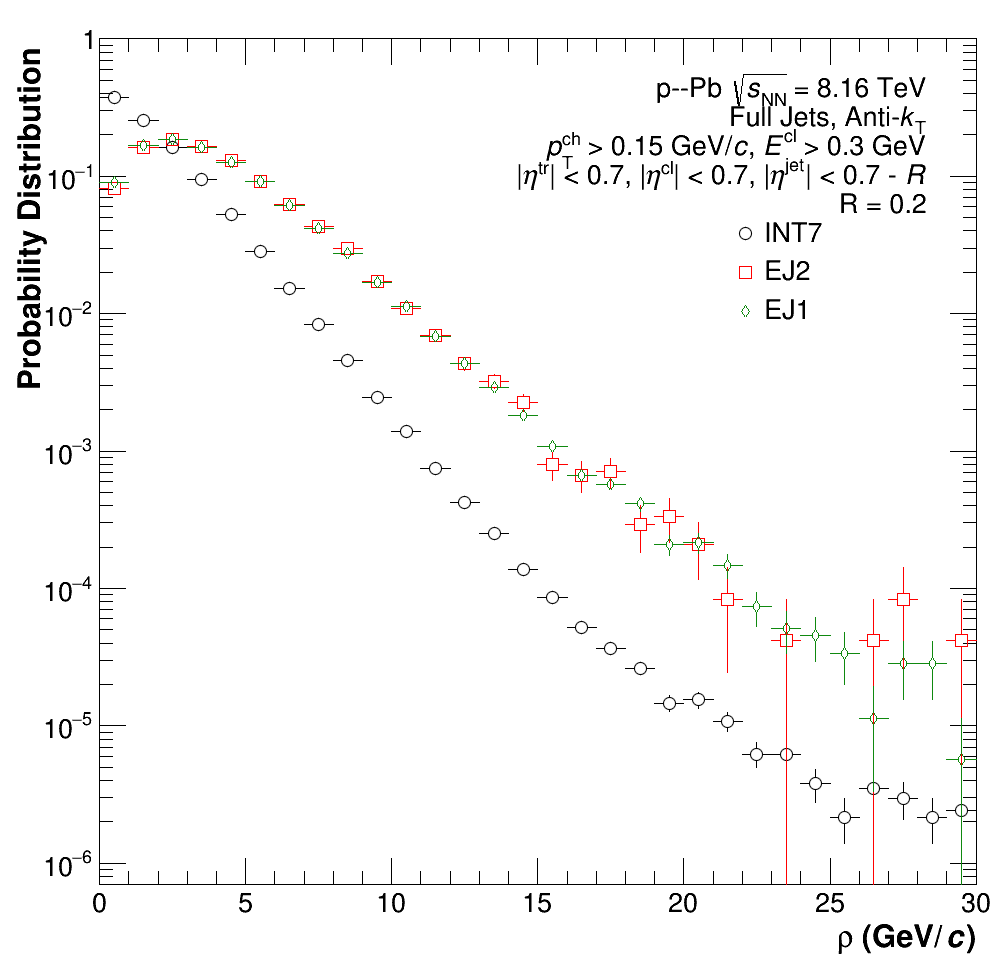
\includegraphics[width=0.49\textwidth]{figures/pPbFigures/BGSubtraction/plotRho_R02.png}
  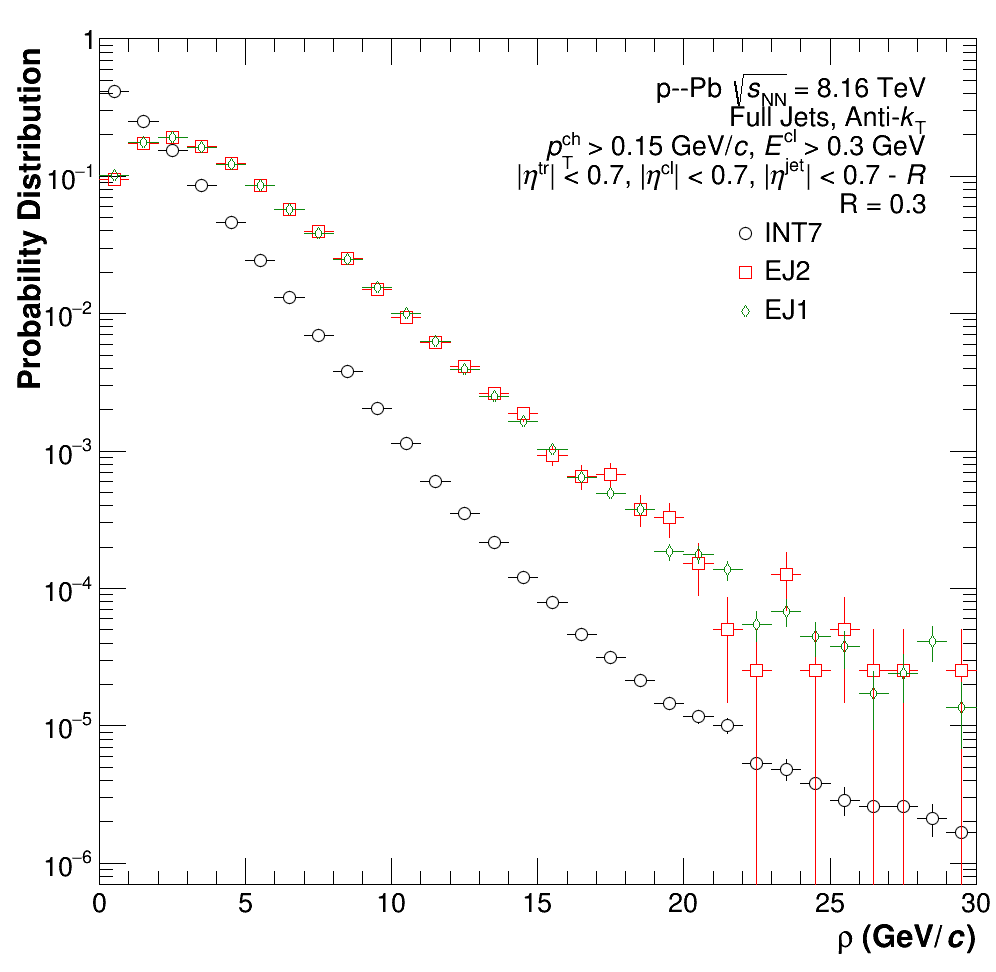
\includegraphics[width=0.49\textwidth]{figures/pPbFigures/BGSubtraction/plotRho_R03.png}
  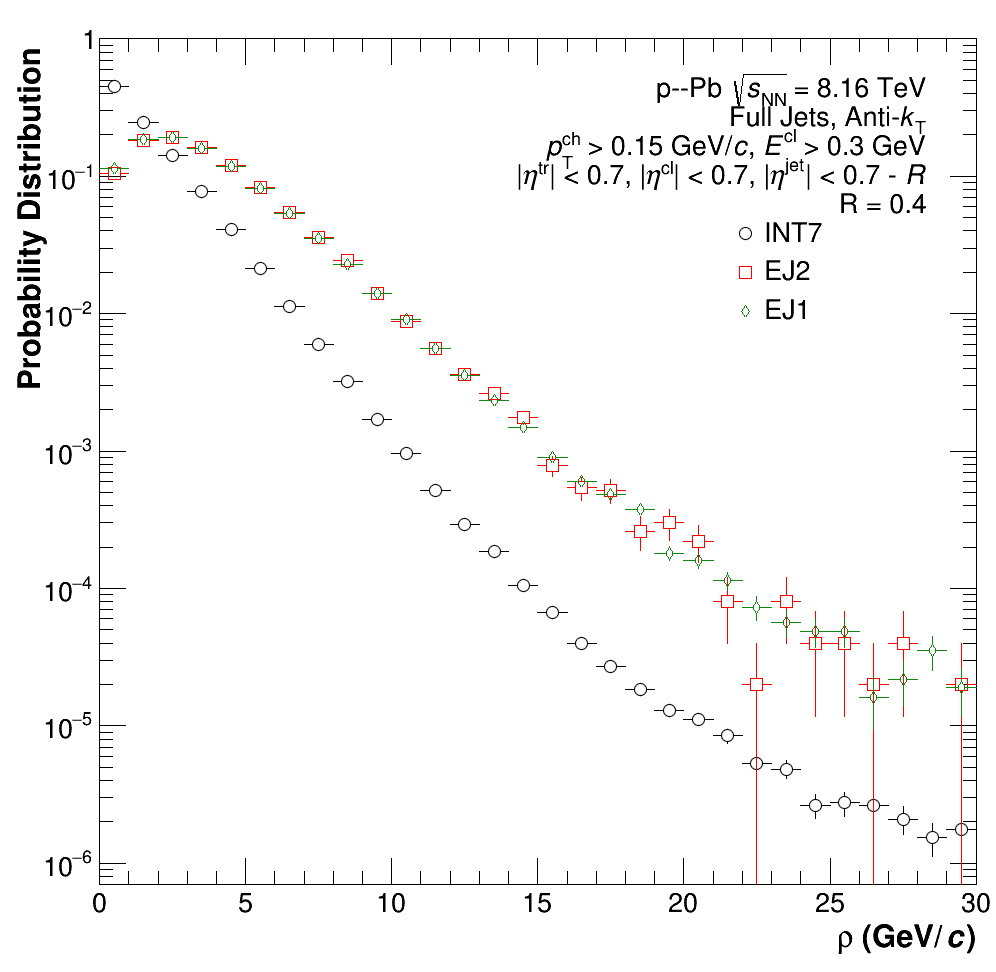
\includegraphics[width=0.49\textwidth]{figures/pPbFigures/BGSubtraction/plotRho_R04.png}
  \caption{Rho distribution for the INT7, EJ2, and EJ1 triggers in \pPb collisions for jets with resolution parameter $R$ = 0.2, 0.3, and 0.4.}
  \label{fig:Rho_distribution}
\end{figure}

The corrected jet momentum is then calculated as 

\begin{equation}
    \text{\pT}_{,jet}^{\text{corr}} = \text{\pT}_{,jet}^{\text{raw}} - \rho_{\text{CMS}} \cdot A_{\text{jet}}.
\end{equation}

\noindent
The background is calculated on an event-by-event basis using only particles within the jet acceptance and assumes a uniform background density. The true background density for each jet fluctuates around this average background density. This effect of background fluctuations is accounted for during the unfolding procedure by first using the random cones approach~\cite{ALICE:2012nbx} to find the $\delta$-\pT distribution. A cone with resolution parameter equivalent to the jet resolution parameter is randomly placed inside the $\eta-\phi$ acceptance of each event. The cone cannot overlap with the highest momentum jet and must be contained within the jet acceptance. The background fluctuations are then defined as 

\begin{equation}
    \delta \text{\pT} = \text{\pT}_\text{,RC} - \rho_{\text{CMS}} \pi R_{\text{cone}}^2
\end{equation}

\noindent
where $\text{\pT}_\text{,RC}$ is the \pT of the random cone and $R_{\text{cone}}$ is its resolution parameter. The $\delta$-\pT distribution for all three triggers is shown in Figure~\ref{fig:DeltaPt_distribution} for jets with resolution parameter $R$ = 0.2, 0.3, and 0.4. The distribution for INT7 is used since this is where the background dominates. The distribution is centered at zero with a steep tail toward negative values caused by fluctuations from soft processes. The longer tail toward positive values originates from both background fluctuations and signal.


\begin{figure}[hbt!]
  \centering
  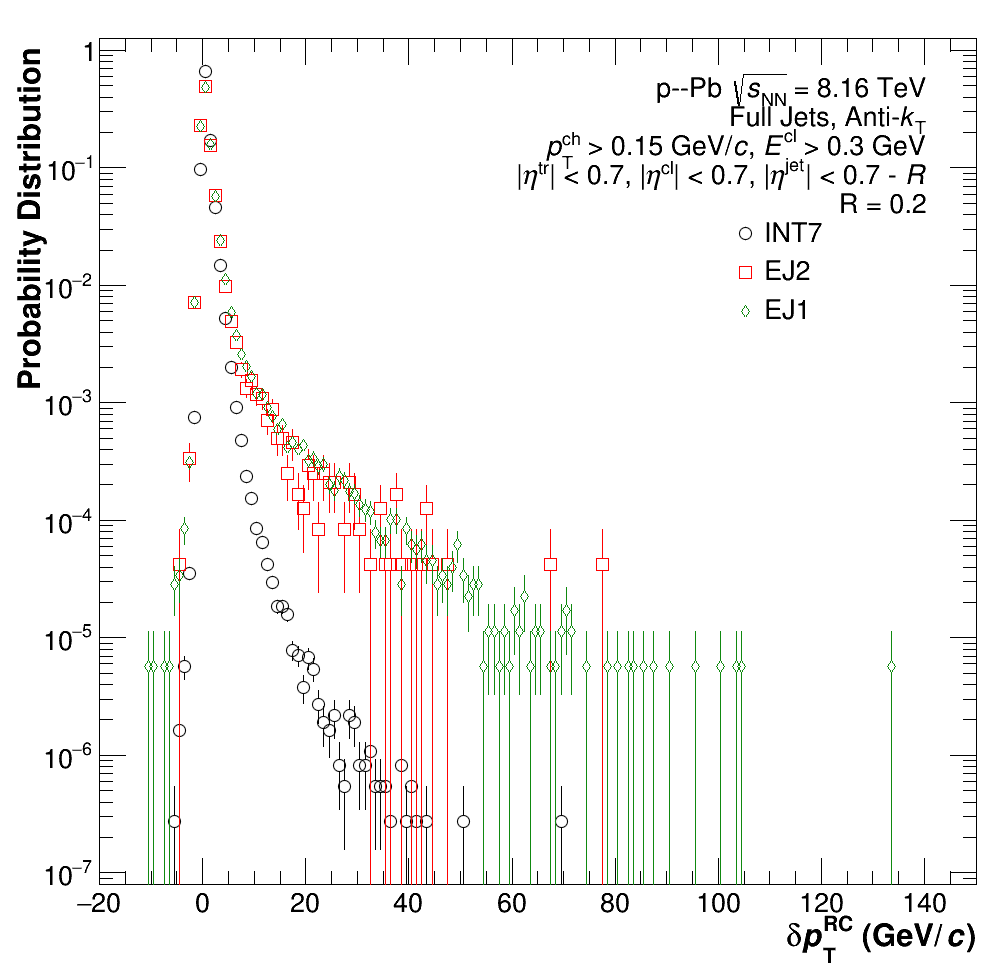
\includegraphics[width=0.49\textwidth]{figures/pPbFigures/BGSubtraction/plotDpT_R02.png}
  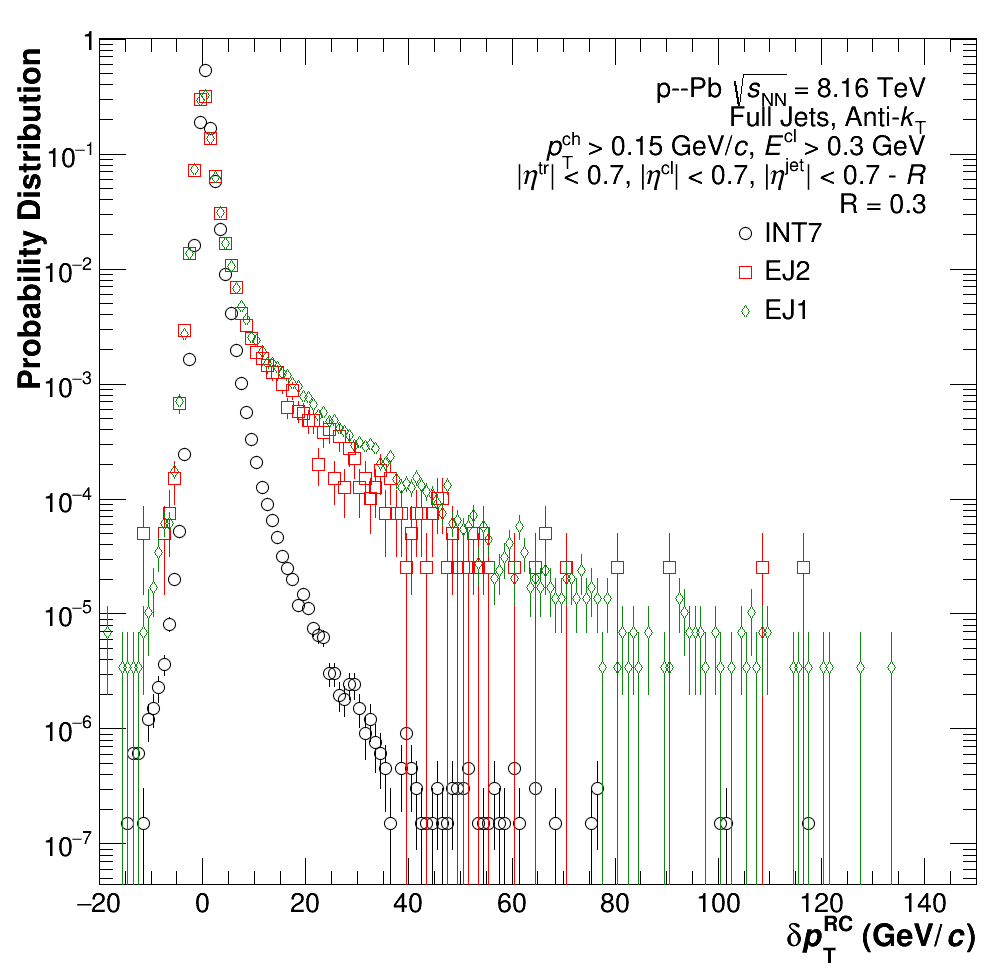
\includegraphics[width=0.49\textwidth]{figures/pPbFigures/BGSubtraction/plotDpT_R03.png}
  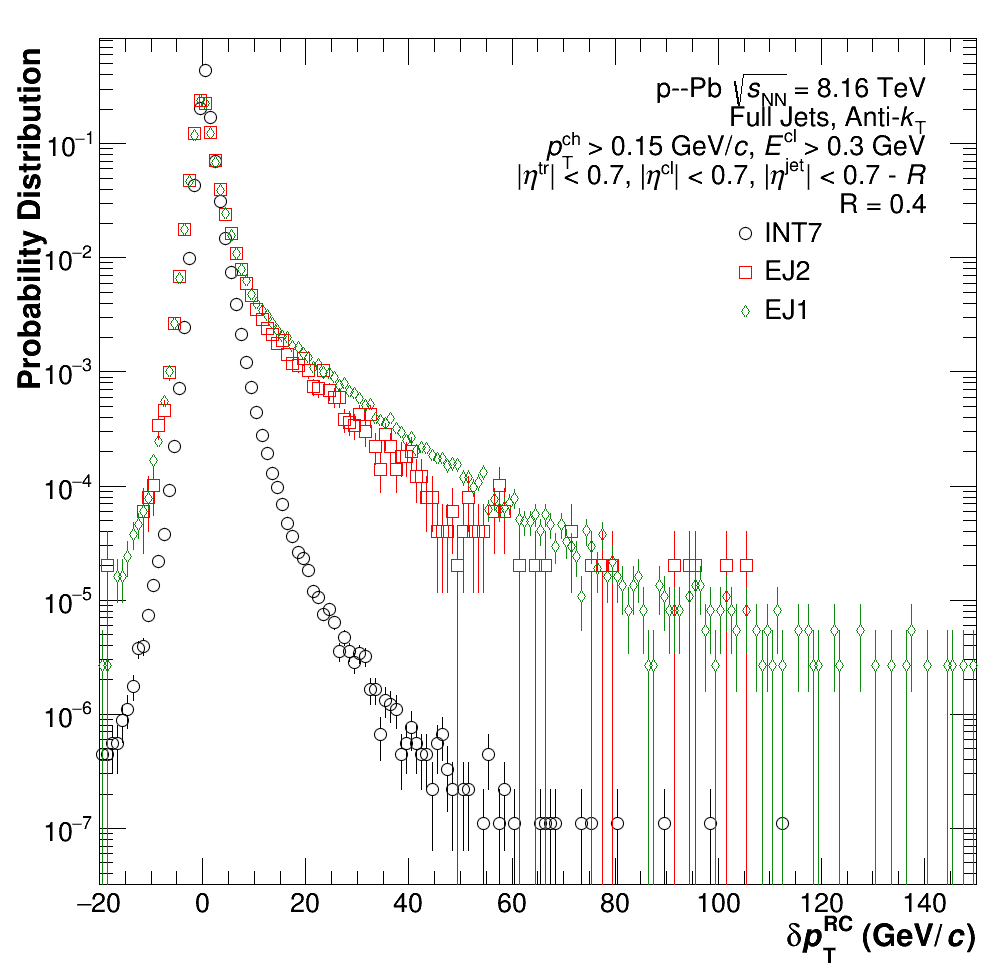
\includegraphics[width=0.49\textwidth]{figures/pPbFigures/BGSubtraction/plotDpT_R04.png}
  \caption{$\delta$-\pT distribution for the INT7, EJ2, and EJ1 triggers in \pPb collisions for jets with resolution parameter $R$ = 0.2, 0.3, and 0.4.}
  \label{fig:DeltaPt_distribution}
\end{figure}

\subsection{Instrumental Response}
\label{sec:InstResponse}


\begin{figure}[hbt!]
    \centering
    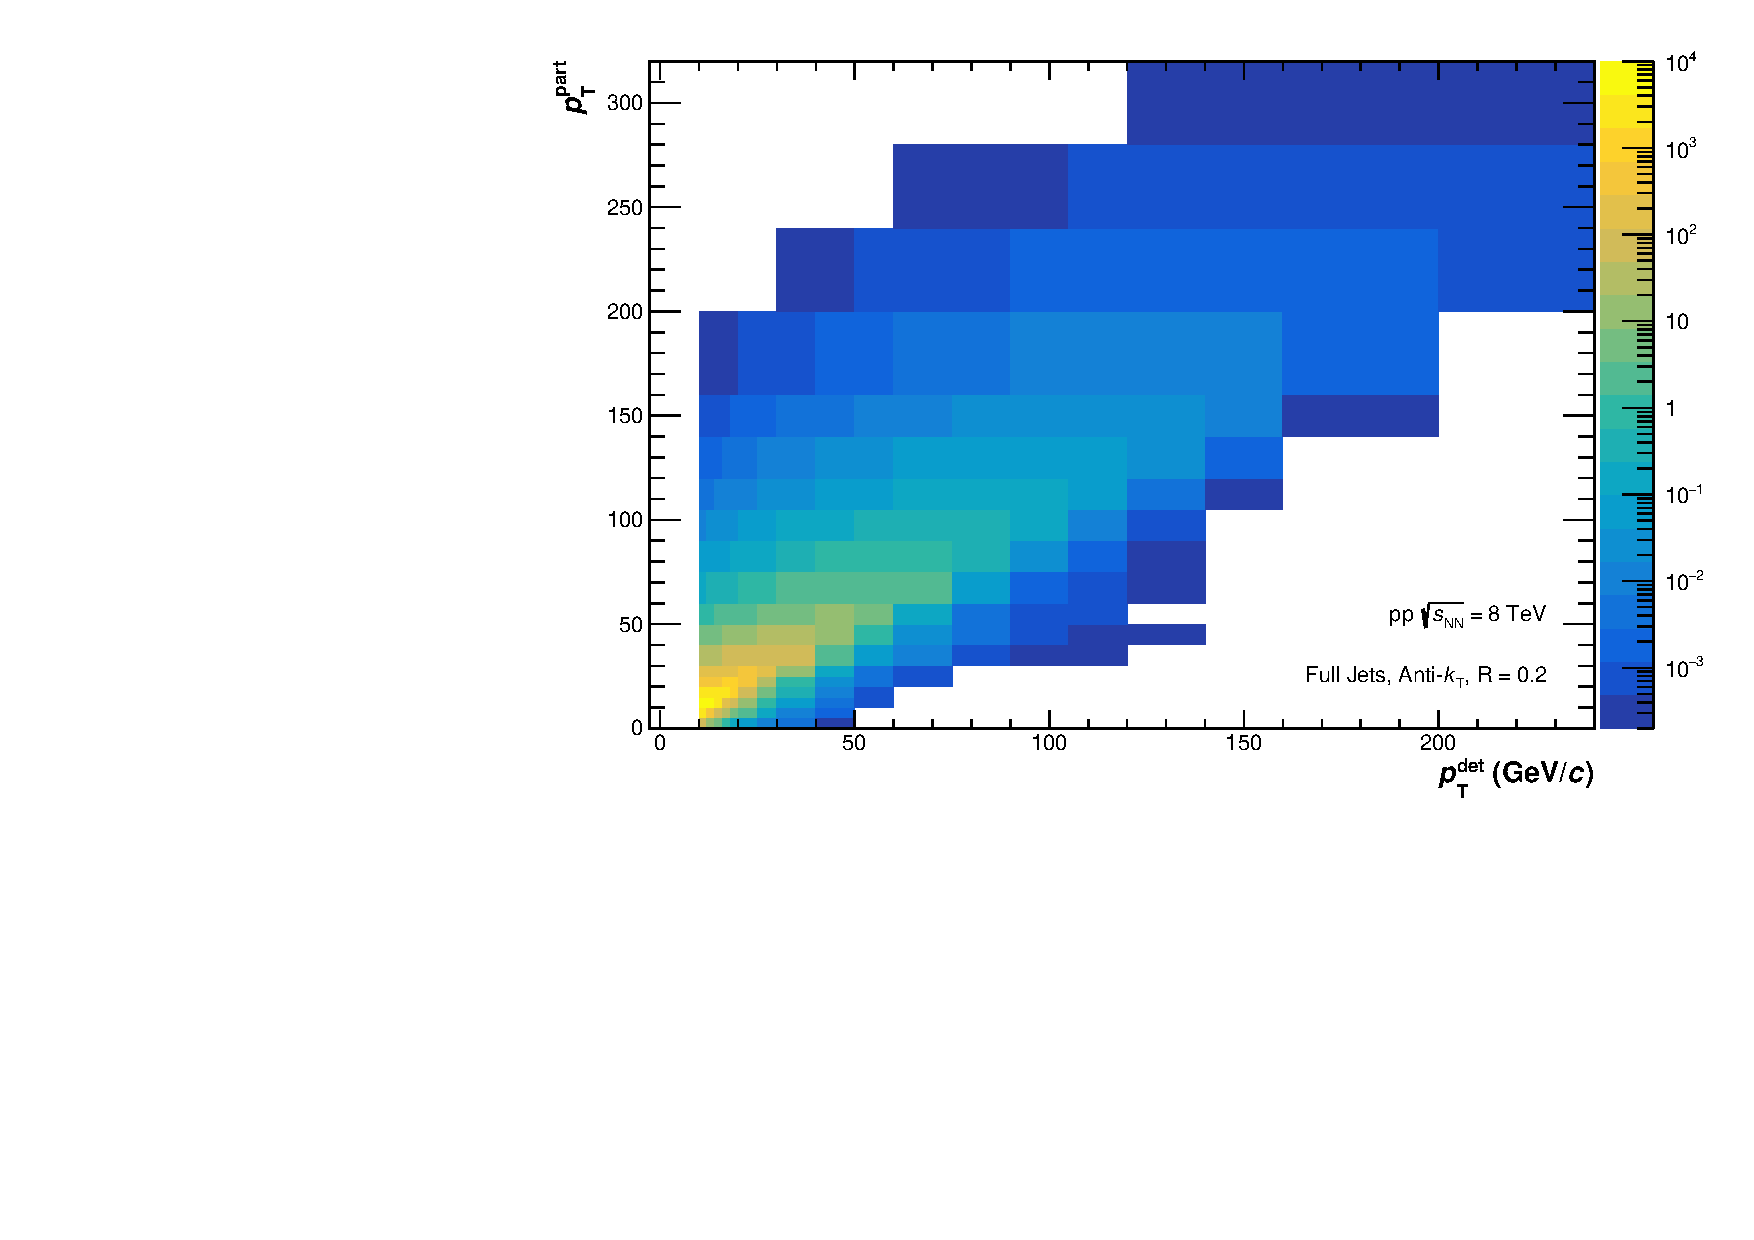
\includegraphics[width=0.95\textwidth]{figures/Response/Response_R02.pdf}
    \caption{Response matrix for \pp collisions for jets with resolution parameter $R$ = 0.2.}
    \label{fig:ResponseMatrix}
\end{figure}

PYTHIA8 events were fully propagated through a simulation of the ALICE detector using GEANT3~\cite{Brun:1987ma} to form a detector response matrix. GEANT is a software package used to simulate particle interactions with detector materials. This response matrix compares jets at generator level (i.e. PYTHIA), typically referred to as "particle level" or "truth level" jets, to jets after propagation through GEANT and reconstruction, typically referred to as "detector level" or "reconstructed level" jets. Detector or reconstructed level is also used to describe data that have not yet been corrected with the response matrix, while particle or truth level is also used to describe data that have been corrected by the response matrix. The response matrix is shown in Figure~\ref{fig:ResponseMatrix} for \pp collisions, which is used to correct the measured jet distributions during unfolding. PYTHIA8 is referred to as the "prior," because by using these simulated events to form the response matrix, an assumption is made that the true jet spectrum looks similar to the jet spectrum produced by PYTHIA8. In order to account for background fluctuations in \pPb events, the response matrix from simulated \pp events at 8.16 TeV was smeared by the $\delta$-\pT distribution from random cones. The residual distribution can be derived in order to characterize the response matrix, which is defined as

\begin{equation}
    \frac{p_\mathrm{T,jet}^{\text{det}} - p_\mathrm{T,jet}^{\text{part}}}{p_\mathrm{T,jet}^{\text{part}}}
\end{equation}

\noindent
where "det" indicates the detector/reconstructed level and "part" indicates the particle/truth level. The residual distribution is used to form the jet energy scale and the jet energy resolution, seen in Figure~\ref{fig:EnergyScale} for \pp and Figure~\ref{fig:EnergyScalepPb} for \pPb. The left plot shows the jet energy scale shift, quantified as the mean of the residual distribution as a function of the true jet \pT. If all jets at particle level were properly reconstructed at detector level, the jet energy scale would be zero. We see a mild $R$ dependence, indicating that jets with a smaller resolution parameter are reconstructed correctly less often than large-$R$ jets. A relative negative shift of around 30\% at $p_\mathrm{T}^\mathrm{jet}$ = 100 GeV/$c$ is present due to finite tracking efficiency. At roughly 60 GeV/$c$, jets are reconstructed correctly more often than at any other \pT. Below this value, the energy scale falls steeply. Above this value, the energy scale decreases gradually toward higher \pT. The right plot shows the jet energy resolution which is quantified as the root mean squared of the distribution of residuals. We observe that the jet energy resolution is relatively flat for fully reconstructed jets at higher \pT due to the contribution from the EMCal. At low \pT, before the EMCal reaches maximum efficiency, the jet energy resolution rises quickly.


\begin{figure}[hbt!]
    \centering
    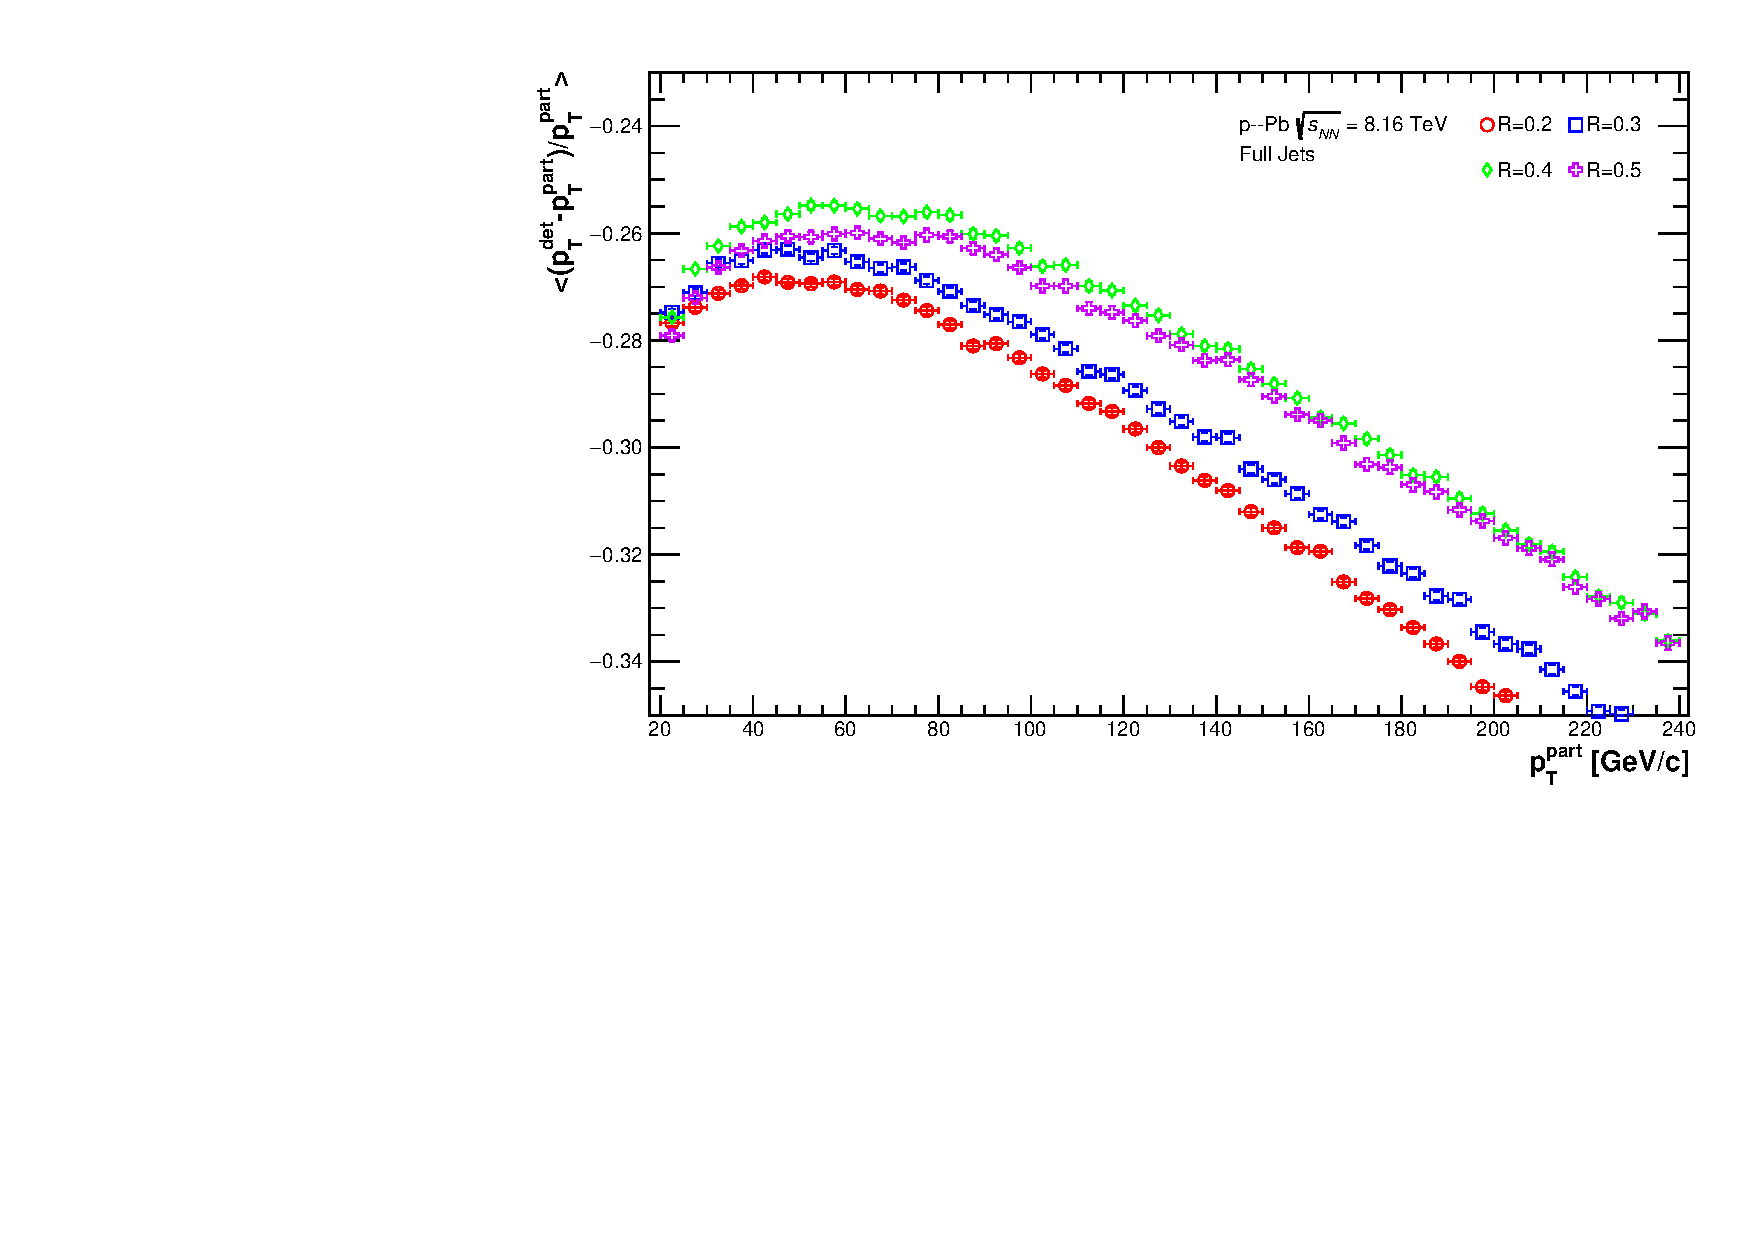
\includegraphics[width=0.49\textwidth]{figures/EnergyScale/EnergyScaleMean.pdf}
    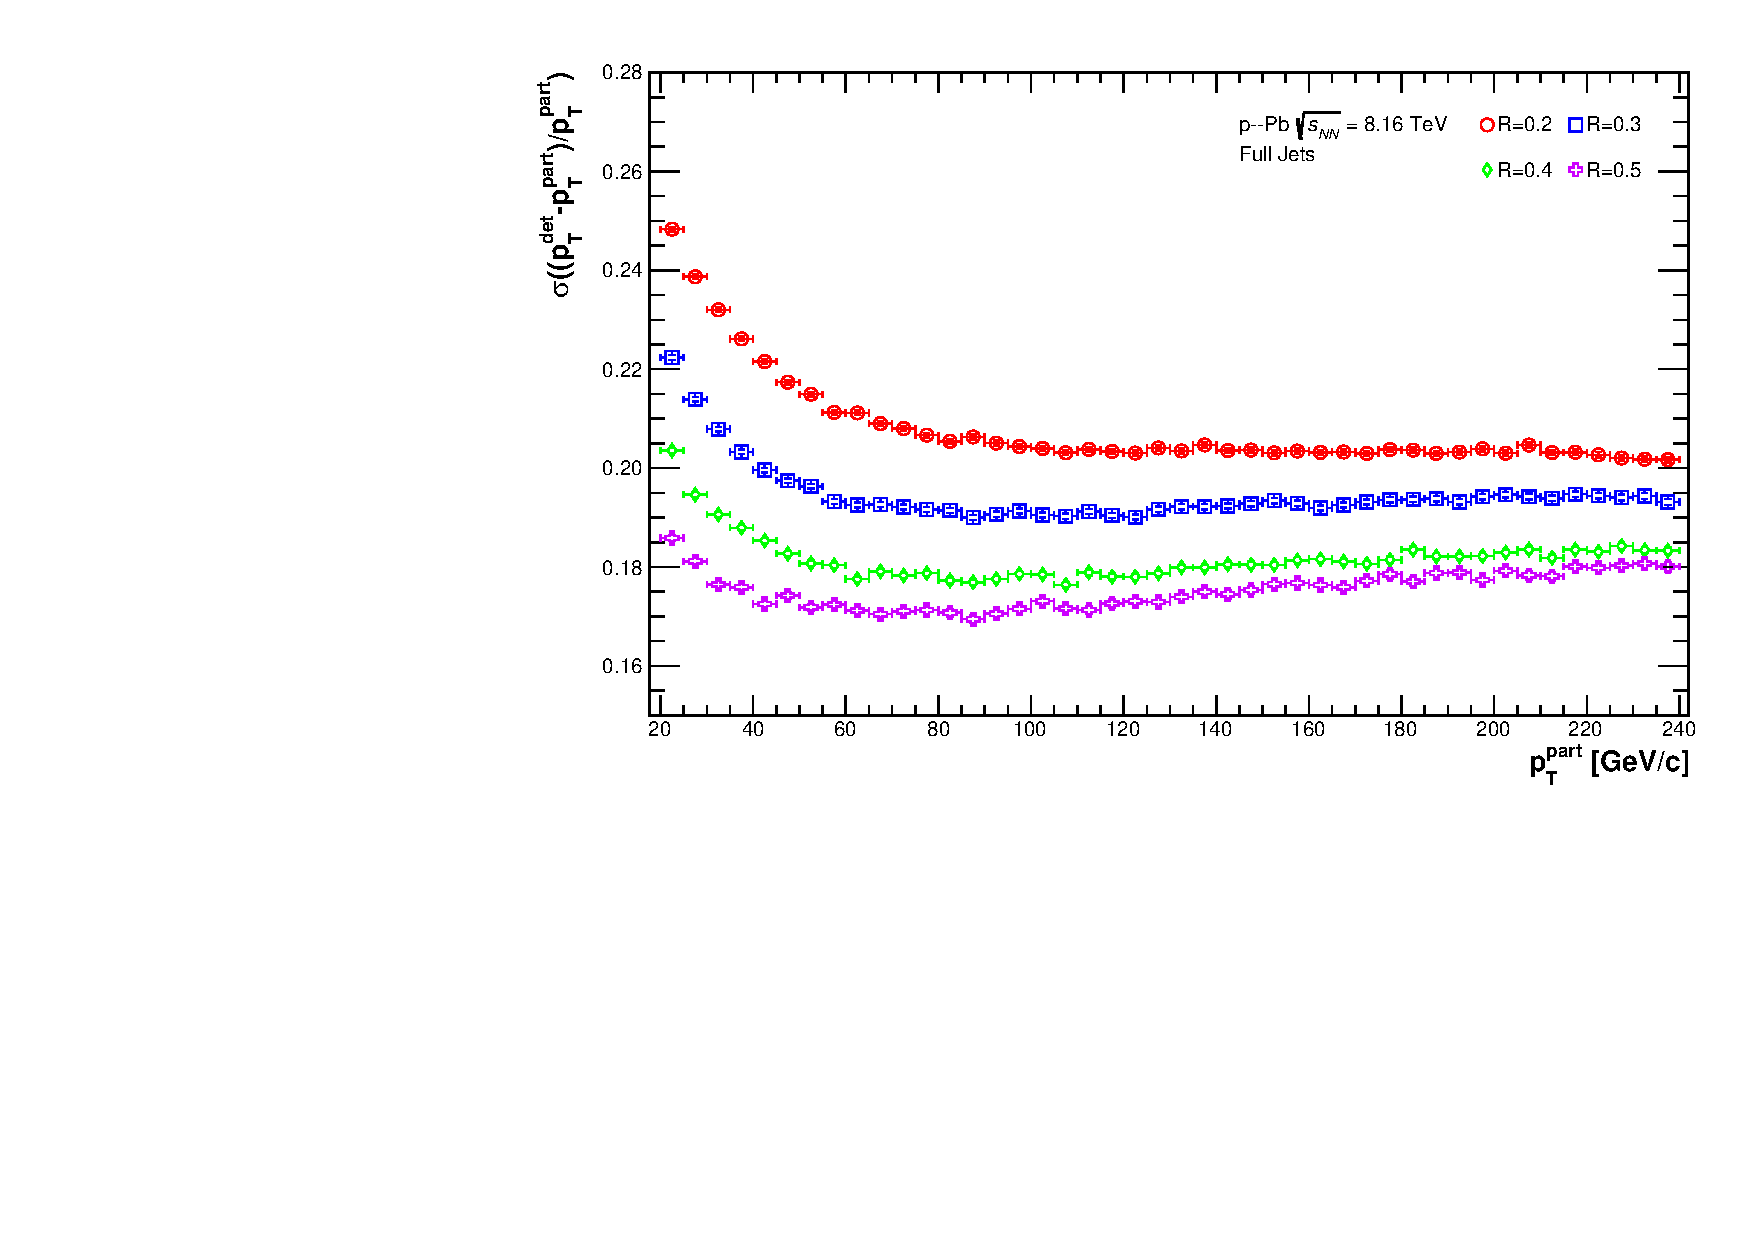
\includegraphics[width=0.49\textwidth]{figures/EnergyScale/EnergyScaleWidth.pdf}
    \caption{Jet energy scale (left) and jet energy resolution (right) showing the instrumental response to jets in \pp collisions.}
    \label{fig:EnergyScale}
\end{figure}

\begin{figure}[hbt!]
    \centering
    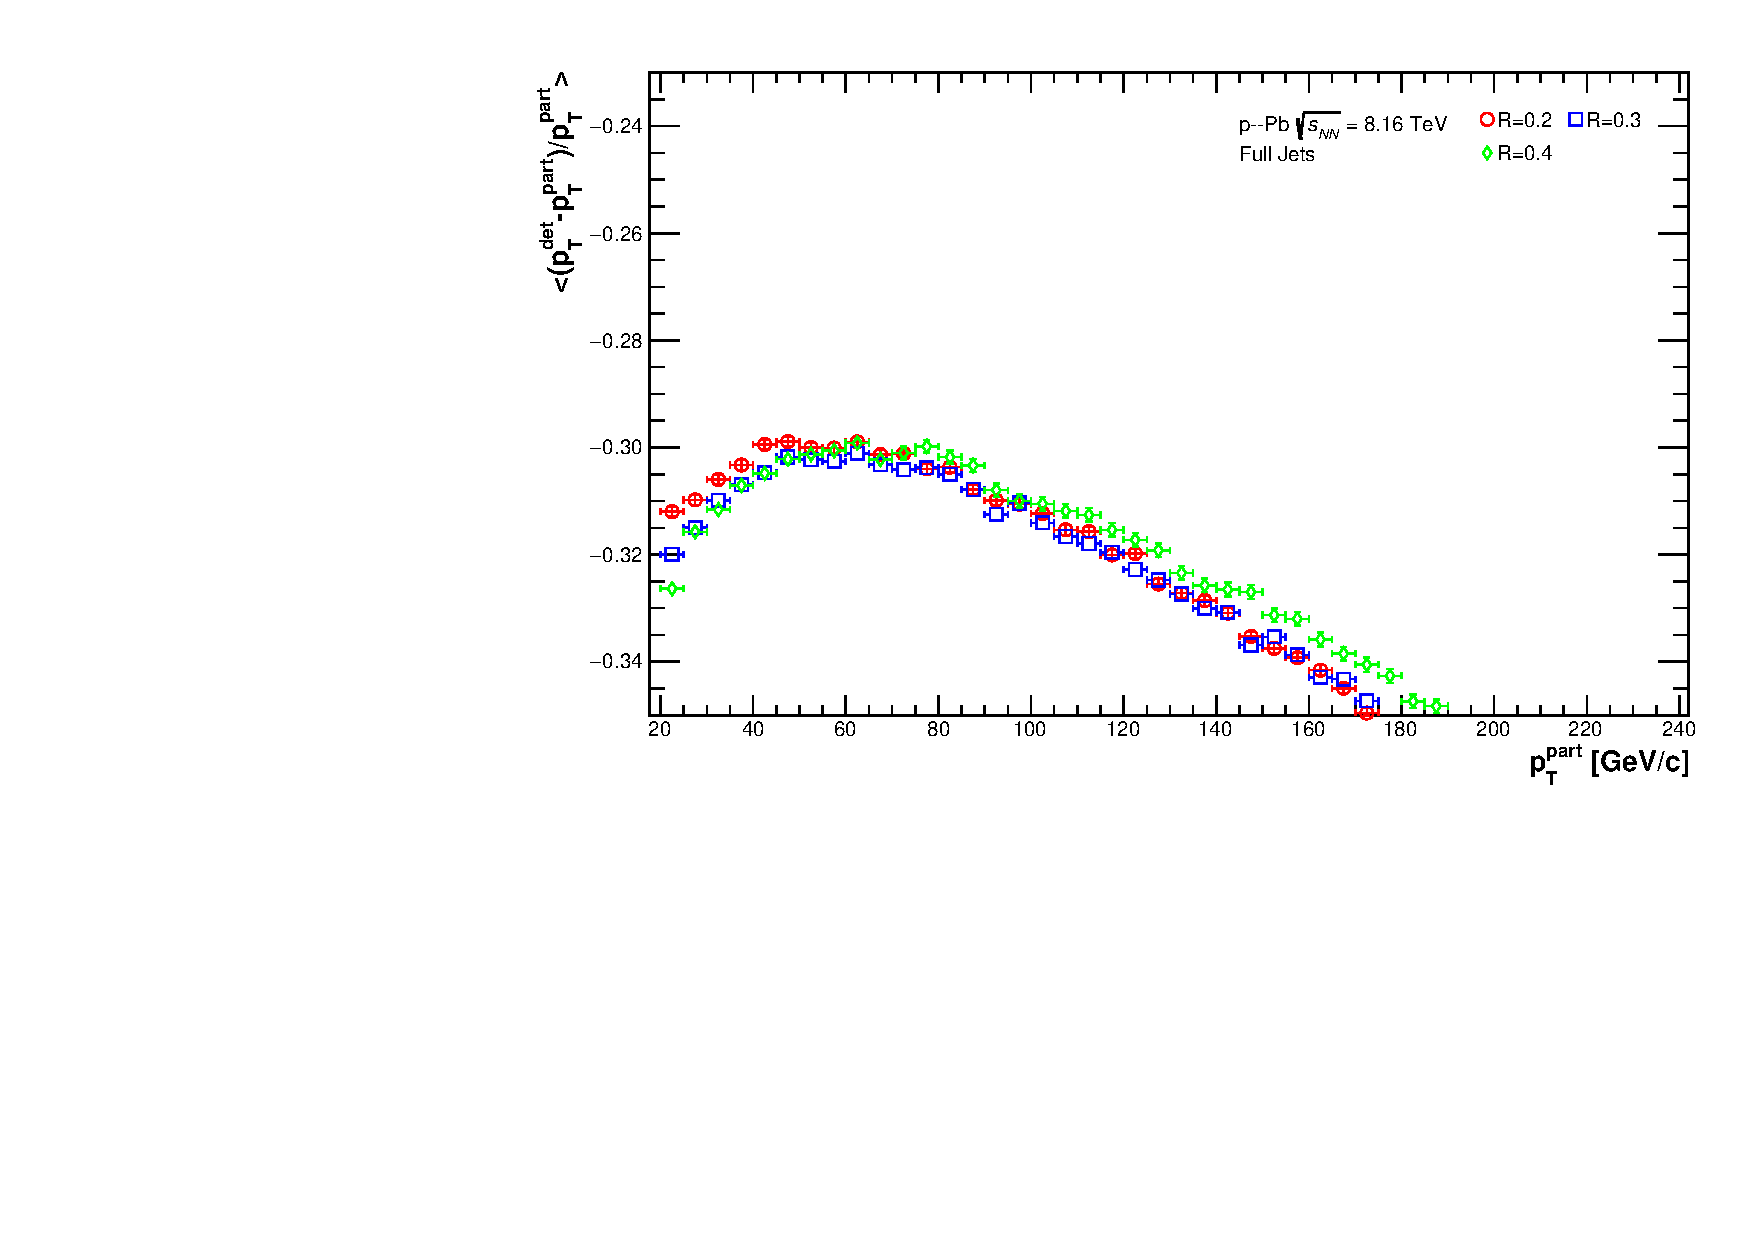
\includegraphics[width=0.49\textwidth]{figures/pPbFigures/EnergyScale/EnergyScaleMean.pdf}
    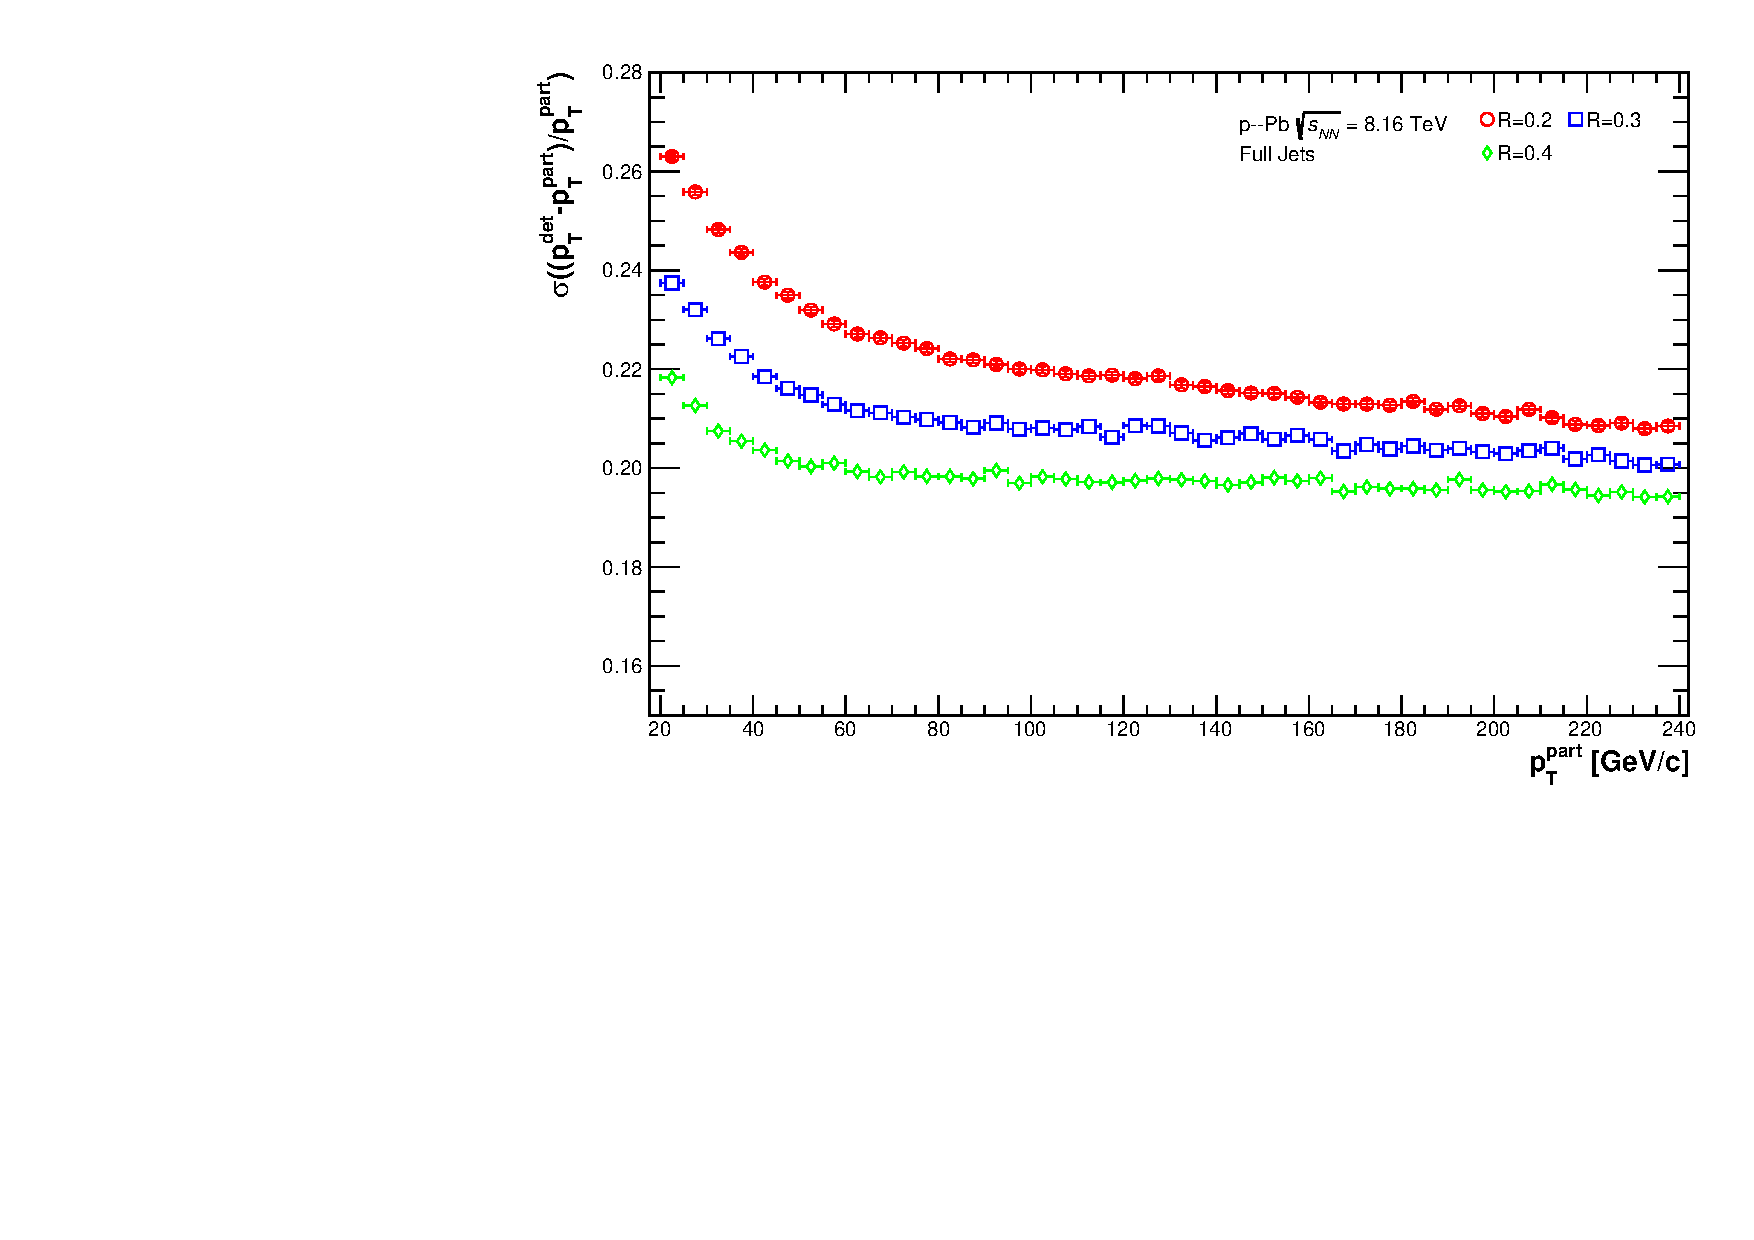
\includegraphics[width=0.49\textwidth]{figures/pPbFigures/EnergyScale/EnergyScaleWidth.pdf}
    \caption{Jet energy scale (left) and jet energy resolution (right) showing the instrumental response to jets in \pPb collisions.}
    \label{fig:EnergyScalepPb}
\end{figure}

For \pp, a comparison to the energy scale results from 13 TeV is also included and can be seen in Figure~\ref{fig:EnergyScaleComp}. The larger the jet resolution parameter, the larger the difference compared to 13 TeV. This is likely due to detector performance effects. The performance during collection of the 13 TeV dataset was significantly different in part from a better resolution due to the inclusion of TRD tracking in approximately 50\% of events. Additionally, there was a smaller fraction of bad channels in the EMCal for run 2. The improvement in jet energy resolution in 13 TeV is greatest at high-\pT. At low-\pT, the resolution overlaps between the two datasets other than in the largest resolution parameter reported.


\begin{figure}[hbt!]
    \centering
    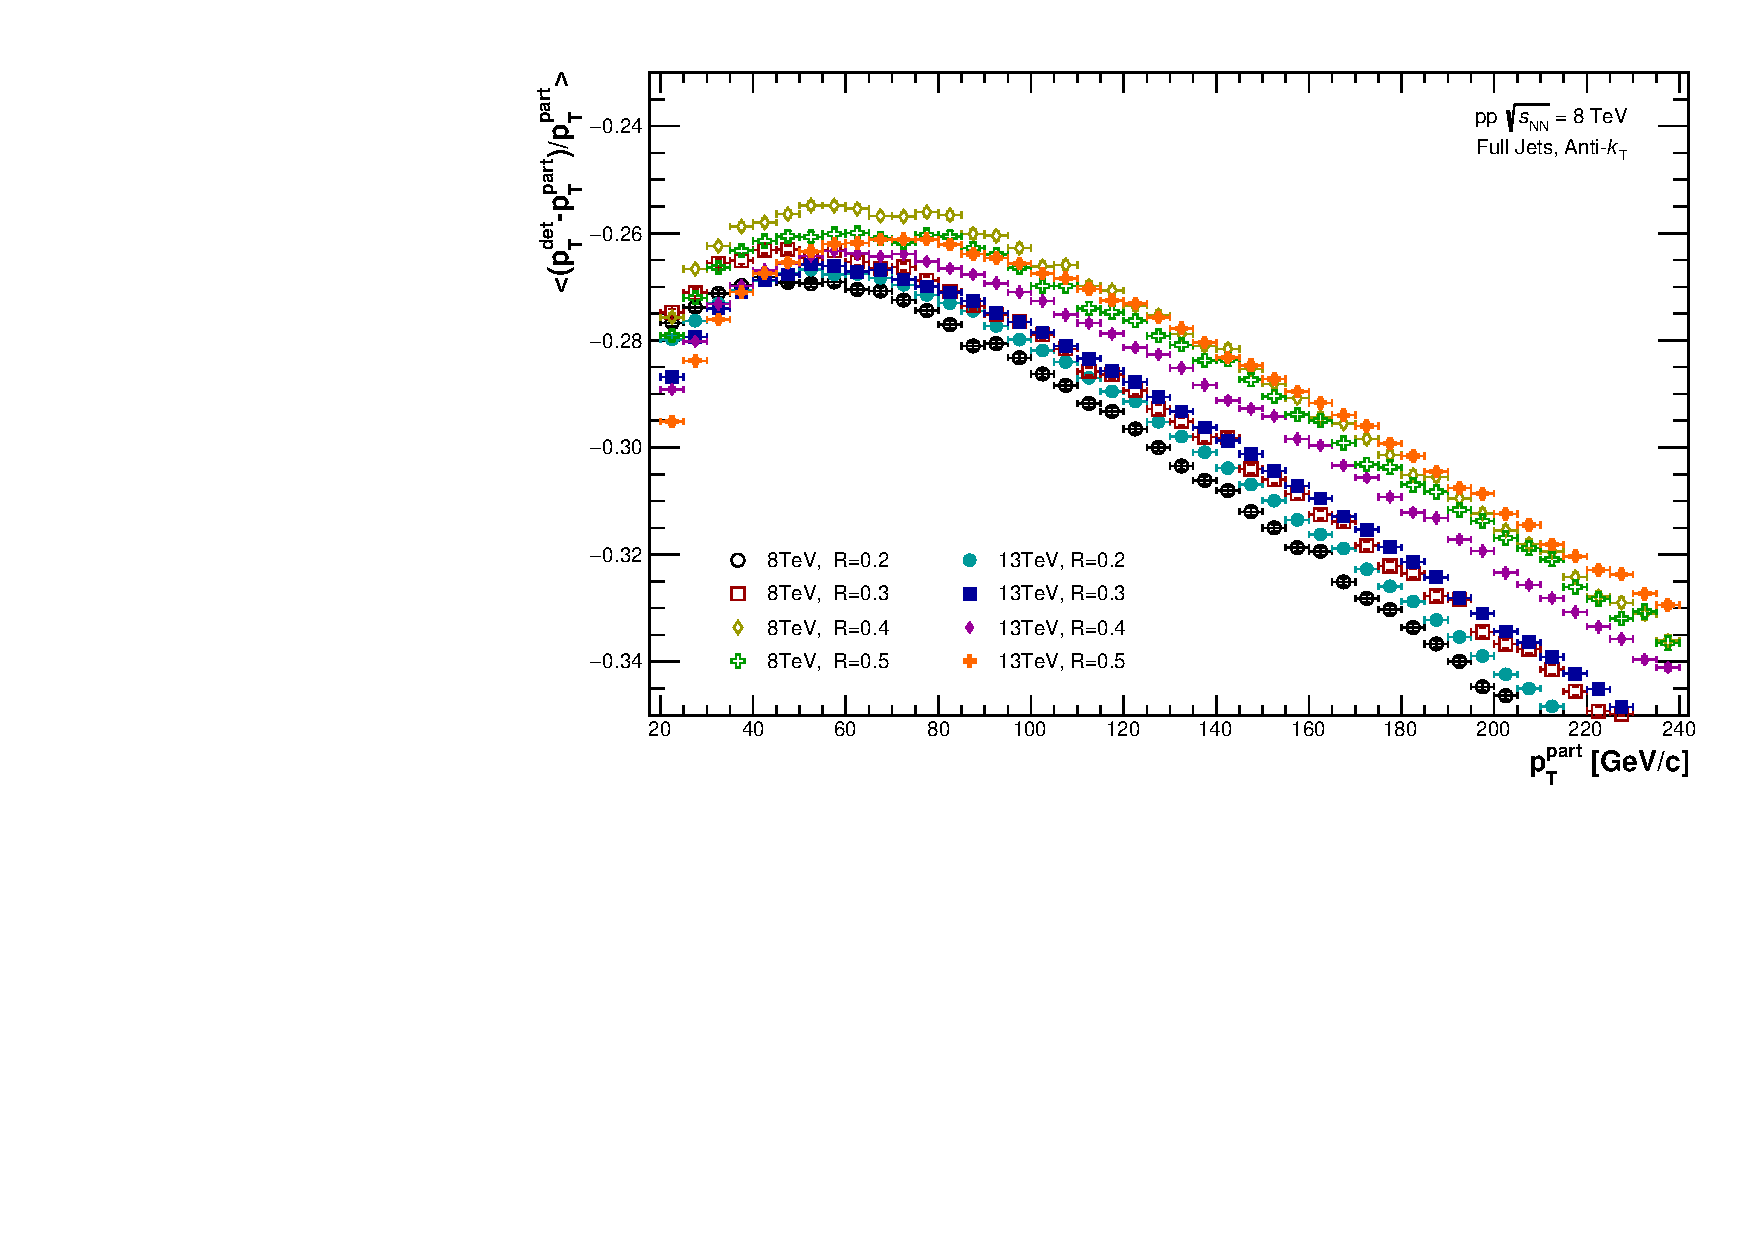
\includegraphics[width=0.49\textwidth]{figures/EnergyScale/EnergyScaleMean_Comparison.pdf}
    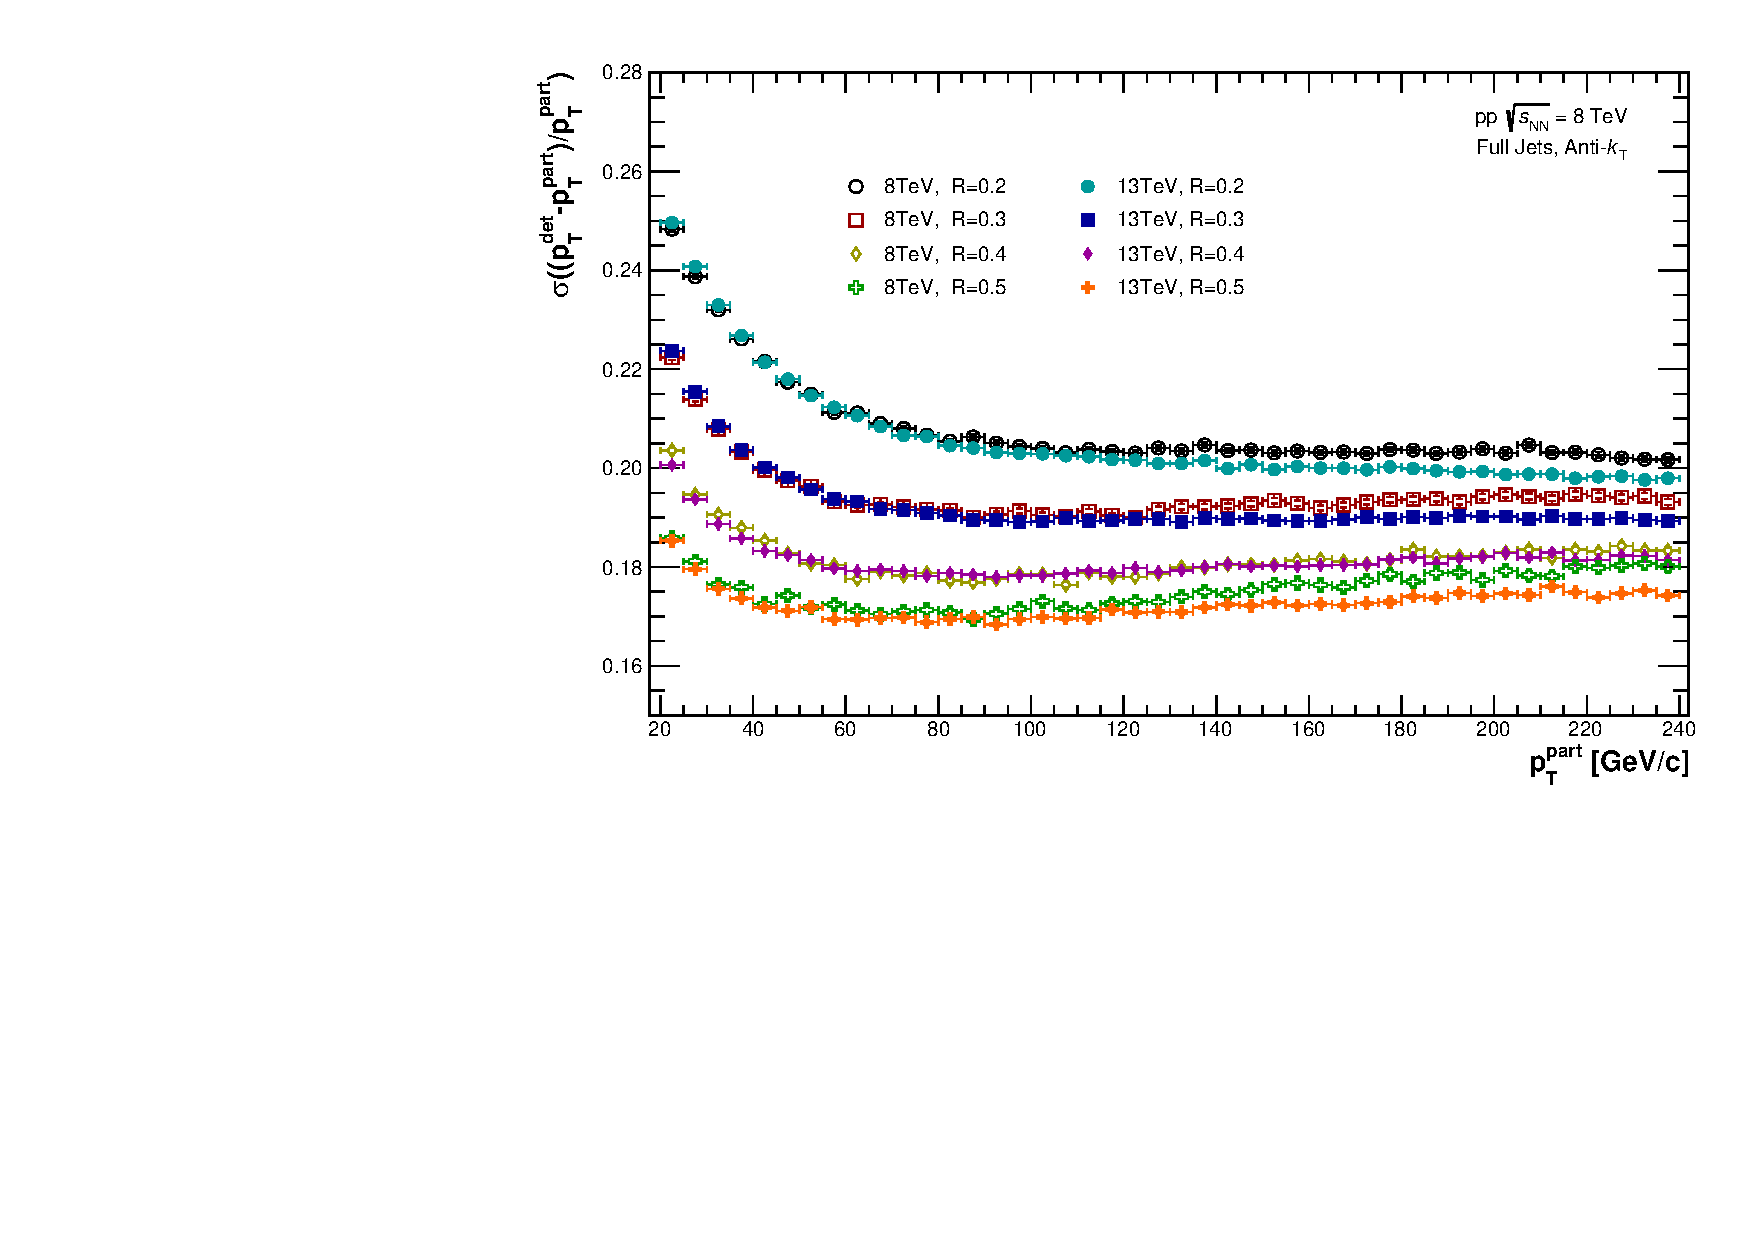
\includegraphics[width=0.49\textwidth]{figures/EnergyScale/EnergyScaleWidth_Comparison.pdf}
    \caption{Jet energy scale (left) and jet energy resolution (right) from the results of this analysis (\pp 8 TeV) compared to those of this analysis of data from \pp collisions at \s = 8 TeV compared to the analysis of jets from \pp collisions at \s = 13 TeV.}
    \label{fig:EnergyScaleComp}
\end{figure}

A different R-ordering can also be seen when comparing the jet energy scale from 8 TeV to that of 13 TeV. For 13 TeV, the energy scale increases with increasing radii from R = 0.2 to 0.6. In 8 TeV, the energy scale increases from R = 0.2 to 0.4, then decreases again for R = 0.5 and R = 0.6. Although the jet energy scale ordering is different, Figure~\ref{fig:eScaleShapeWidth} shows that the shape of the distributions is comparable, but energy resolution is slightly worse for 8 TeV.


\begin{figure}[hbt!]
    \centering
    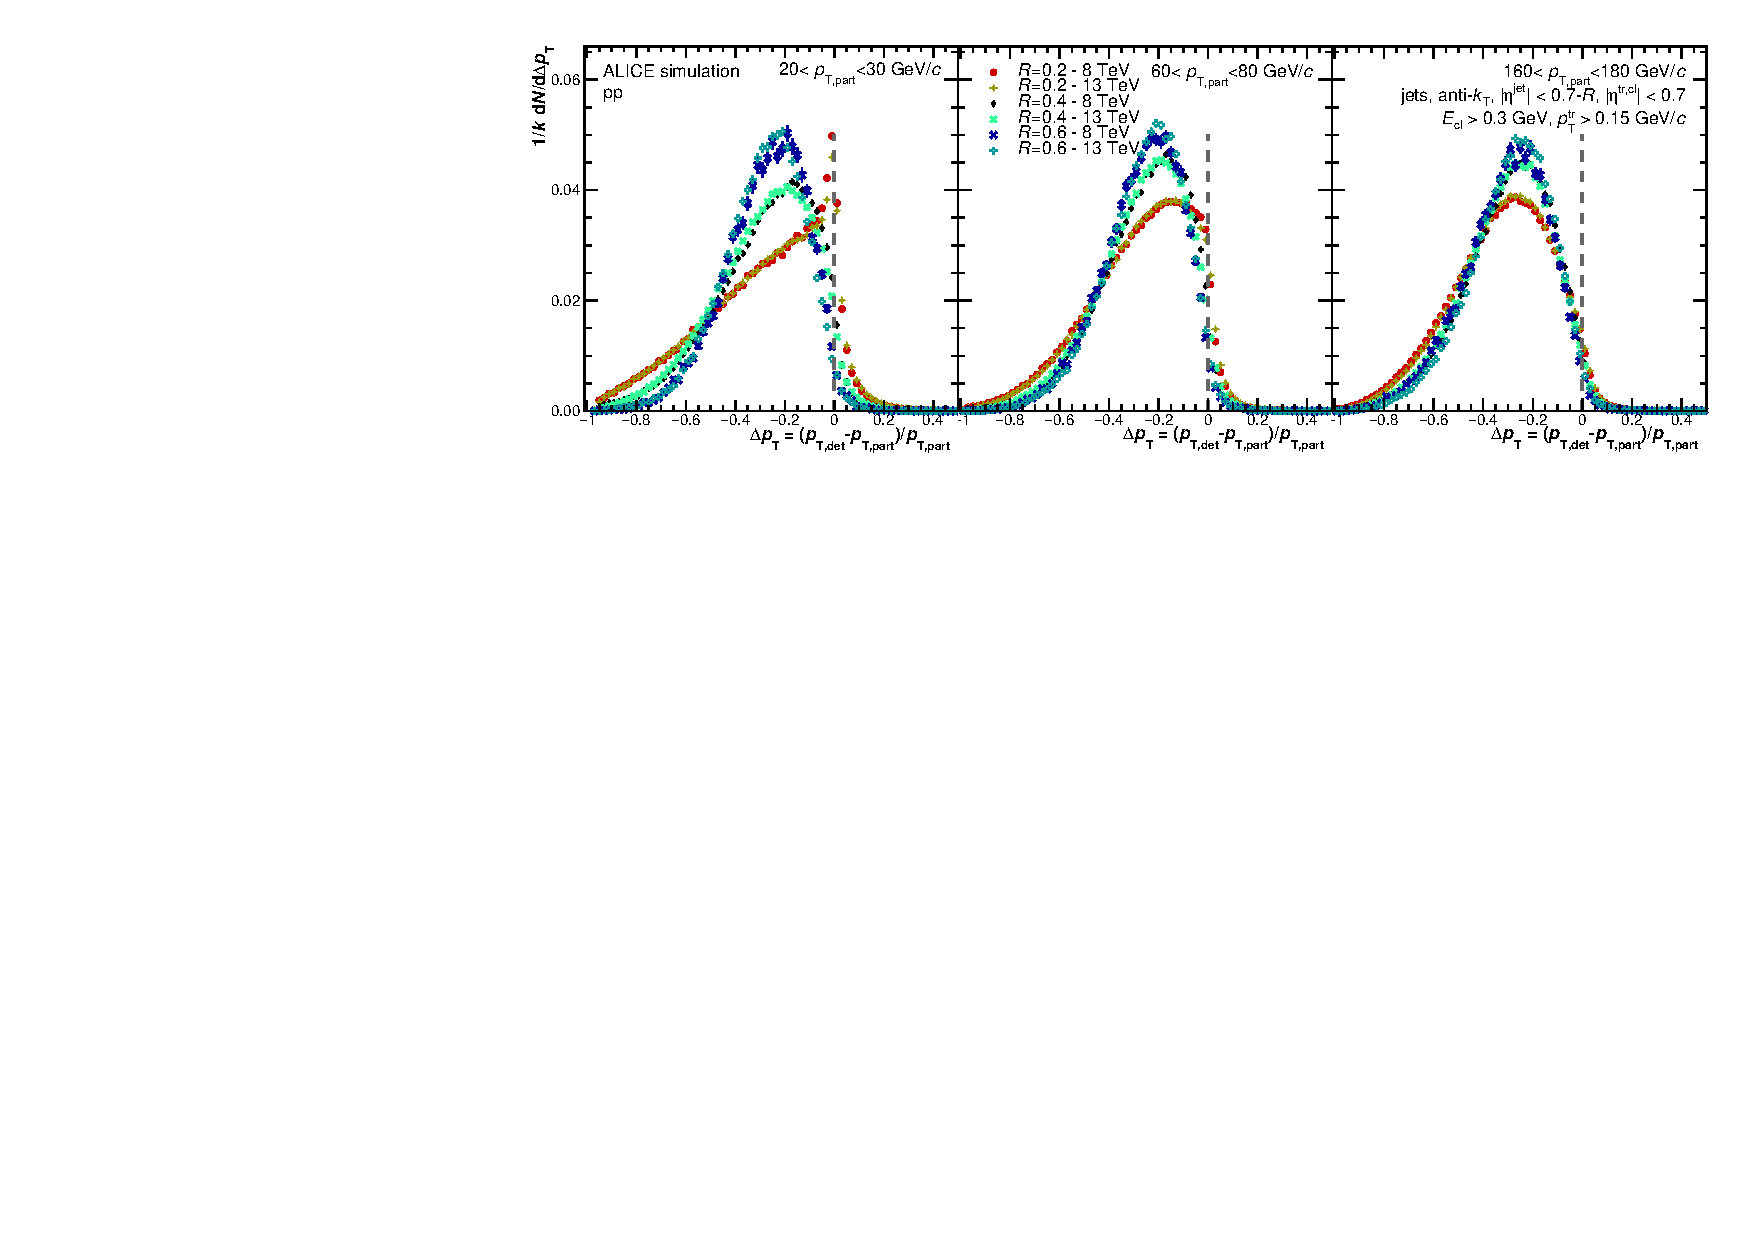
\includegraphics[width=\textwidth]{figures/EnergyScale/ROrdering/JetEscaleProj_3_EnergyComp.pdf}
    \caption{Jet energy scale projections showing the shape of the distributions for 8 and 13 TeV in \pp collisions.}
    \label{fig:eScaleShapeWidth}
\end{figure}

To explore the discrepancy, the jet energy scale is broken down into its charged track and EMCal cluster components, which will be referred to as the charged and neutral components, seen in Figure~\ref{fig:eScaleChNe}. The R-ordering difference is seen for both components, but is greater for the neutral component. In 2012, there was acceptance loss for the charged component due to dead areas in the SPD tracking, and the ITS-TPC track matching was different as a function of $\phi$. Charged particles that pass through these areas will not result in SPD clusters, and thus will not produce an SPD tracklet. The larger the jet resolution parameter, the more likely it is for tracks contained within the jet cone to overlap with these dead areas. The more a jet overlaps with dead areas, the greater the difference between particle and detector level. This effect was not present for the majority of the runs, which is evident by the smaller impact compared to the neutral component. The neutral component is also impacted by the partially installed TRD in 2012. Some of the EMCal supermodules had TRD material in front of them, while others did not. The larger the jet resolution parameter, the more likely it was to cross boundaries in the EMCal between where there was and was not TRD material. As is the case for the dead areas of the SPD, jets overlapping with the TRD will have less of the jet energy reconstructed at detector level. Example plots showing tracking and EMCal occupancy as a function of $\eta$ and $\phi$ can be seen in Figure~\ref{fig:eScaleTracksClusters}. The R-ordering effect observed for \pp collisions at 8 TeV is not seen for \pPb collisions at 8.16 TeV. The \pPb data were recorded during run 2 and benefit from the same improved detector conditions as \pp collisions at 13 TeV.


\begin{figure}[hbt!]
    \centering
    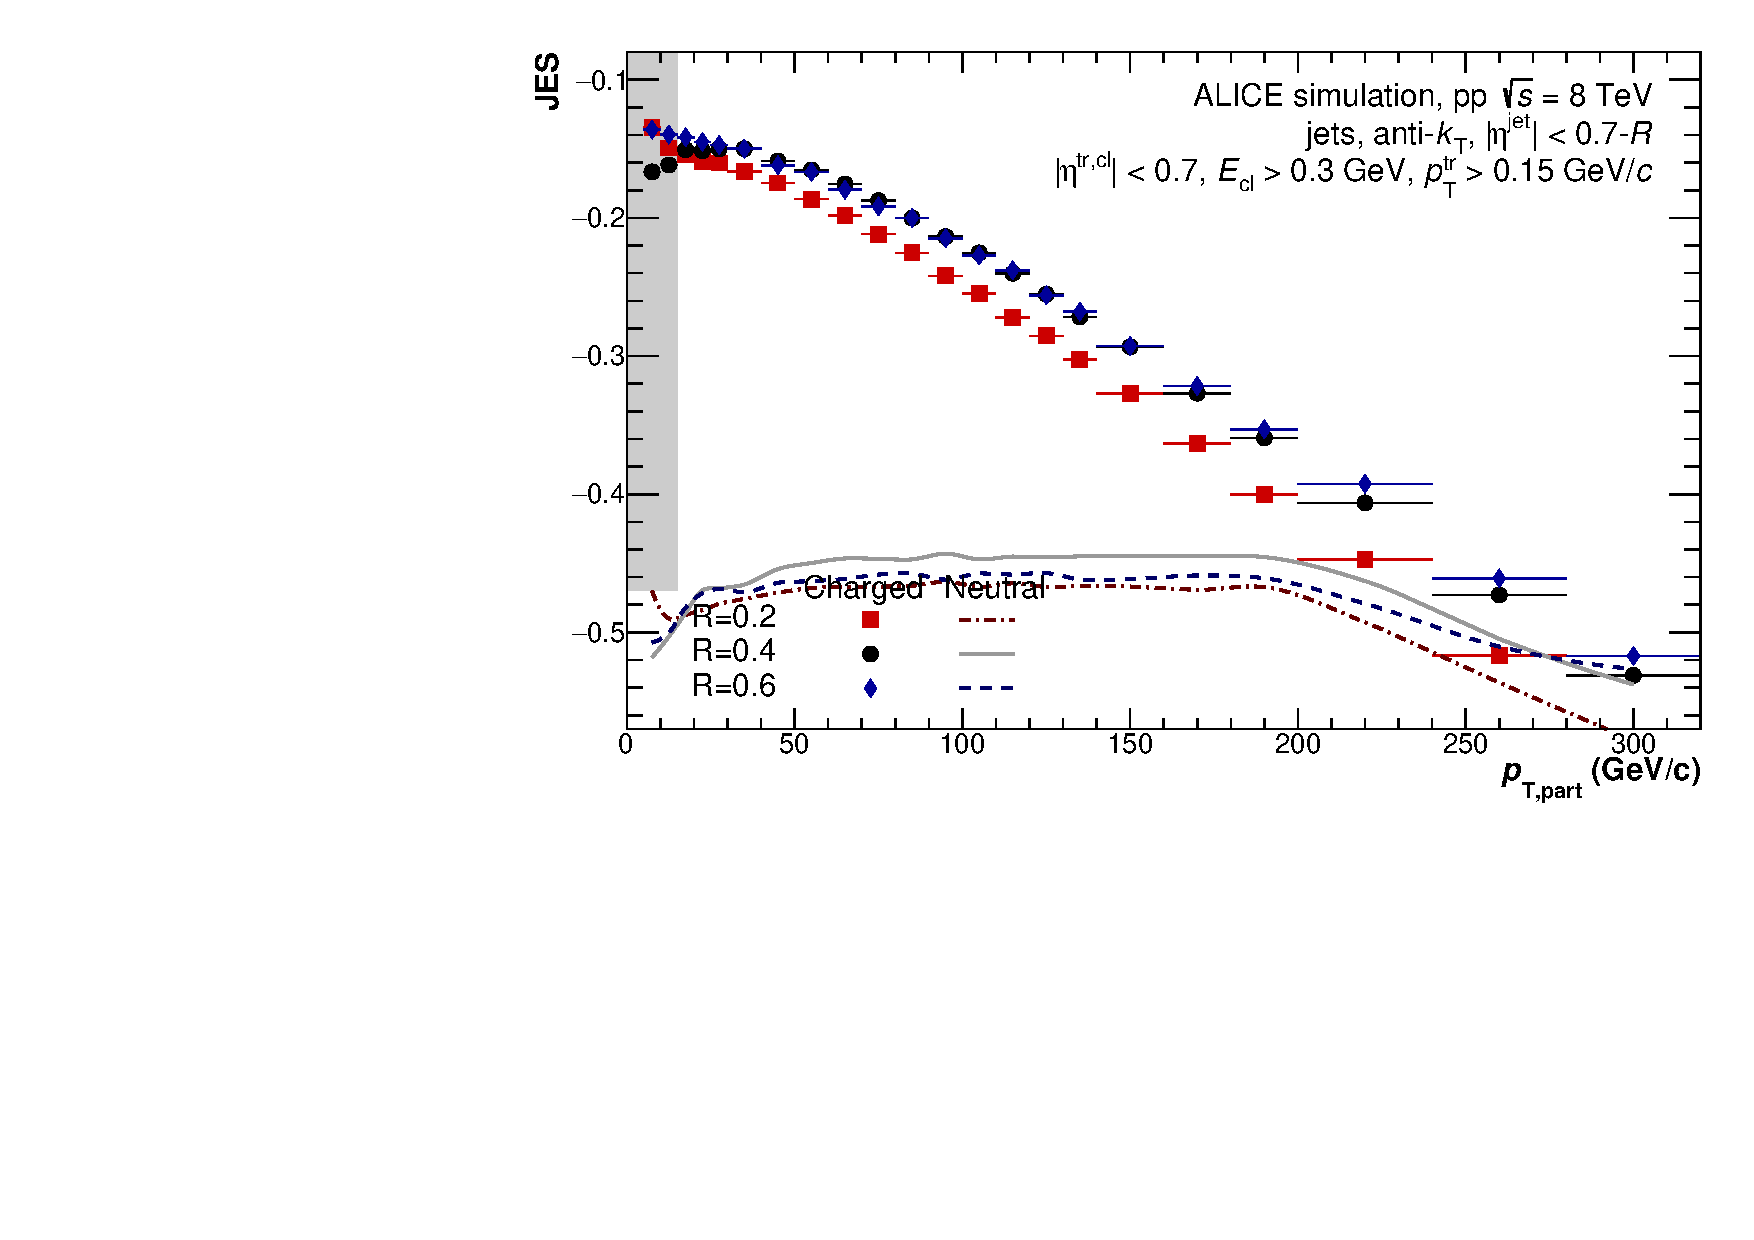
\includegraphics[width=0.75\textwidth]{figures/EnergyScale/ROrdering/JES_8_3_ChNe.pdf}
    \caption{Jet energy scale broken up into its charged and neutral components.}
    \label{fig:eScaleChNe}
\end{figure}


\begin{figure}[hbt!]
    \centering
    %\subfigure{
        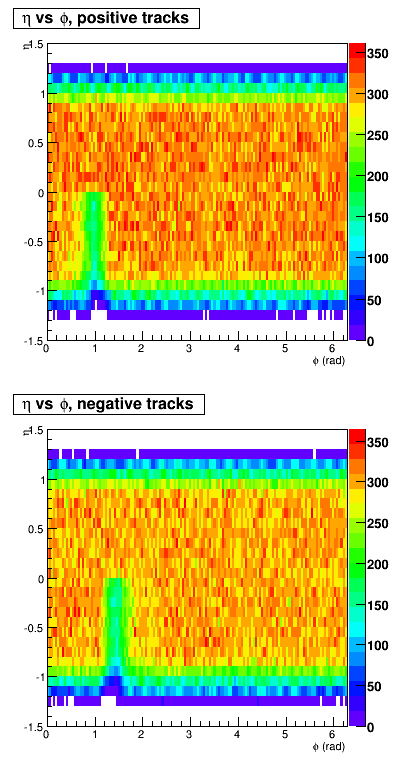
\includegraphics[width=0.35\textwidth]{figures/EnergyScale/ROrdering/spd_holes.png}
    %}
    %\subfigure{
        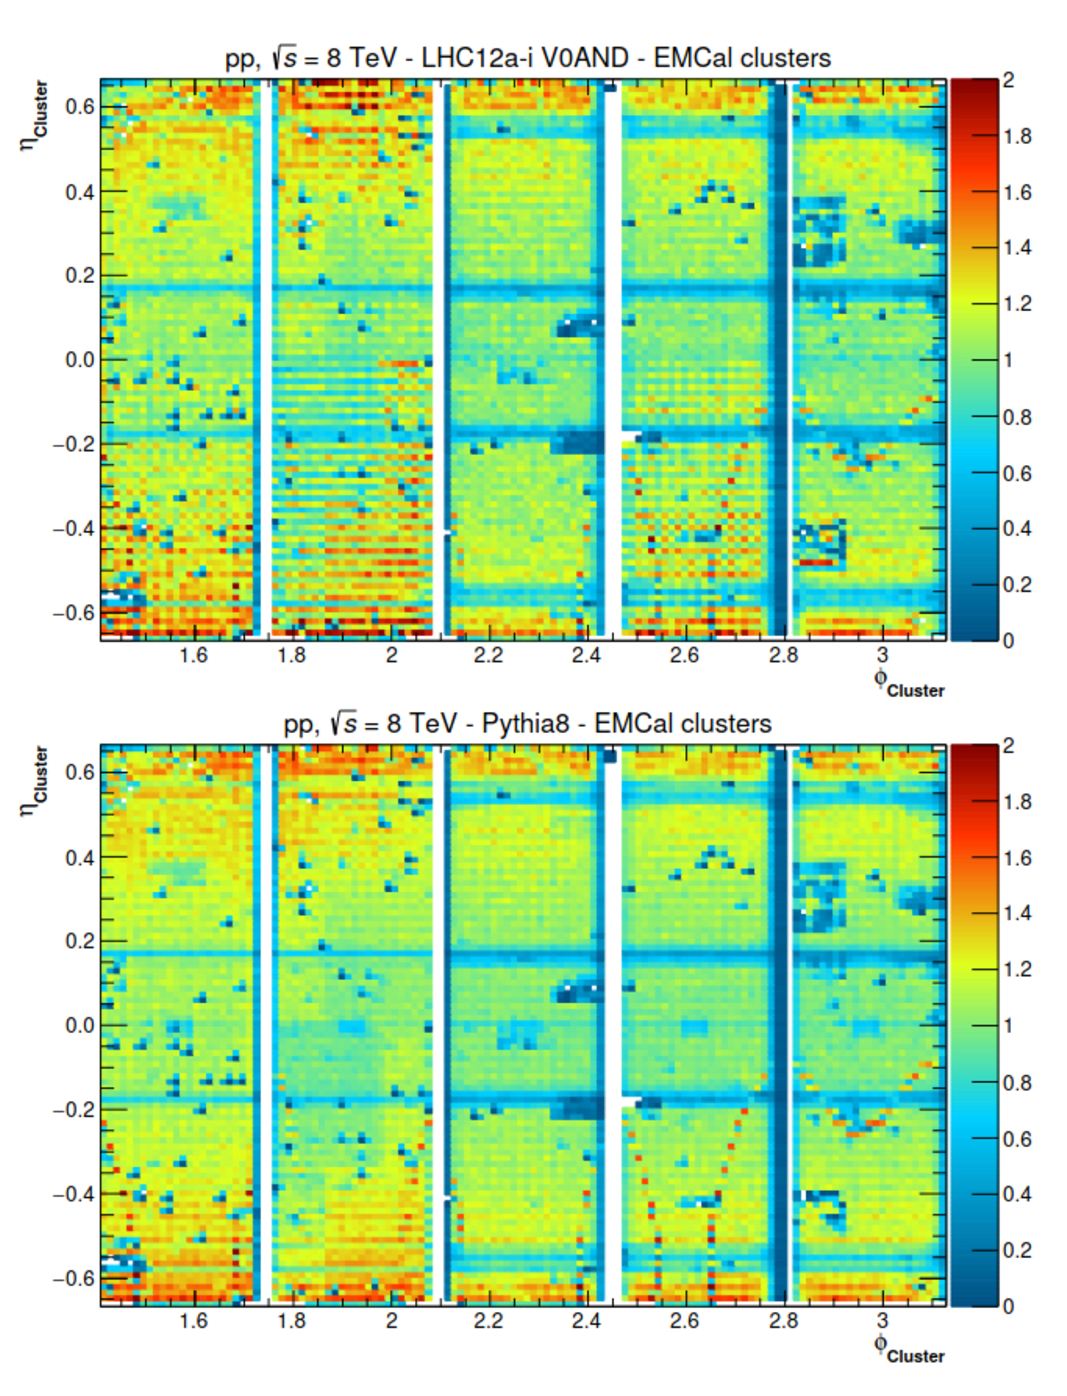
\includegraphics[width=0.5\textwidth]{figures/EnergyScale/ROrdering/emcal_occupancy_cropped.eps}
    %}
    \caption{TPC-ITS track distribution (left) and EMCal cluster distribution (right) as a function of $\eta$ and $\phi$. The top right plot shows the EMCal cluster distribution for the V0AND minimum bias trigger in the 2012 dataset, while the bottom right plot shows the EMCal cluster distribution for the same dataset modeled by PYTHIA8 propagated though a GEANT simulation of the detector.}
    \label{fig:eScaleTracksClusters}
\end{figure}

\subsection{Kinematic efficiency}
\label{sec:kinEff}


\begin{figure}[hbt!]
    \centering
    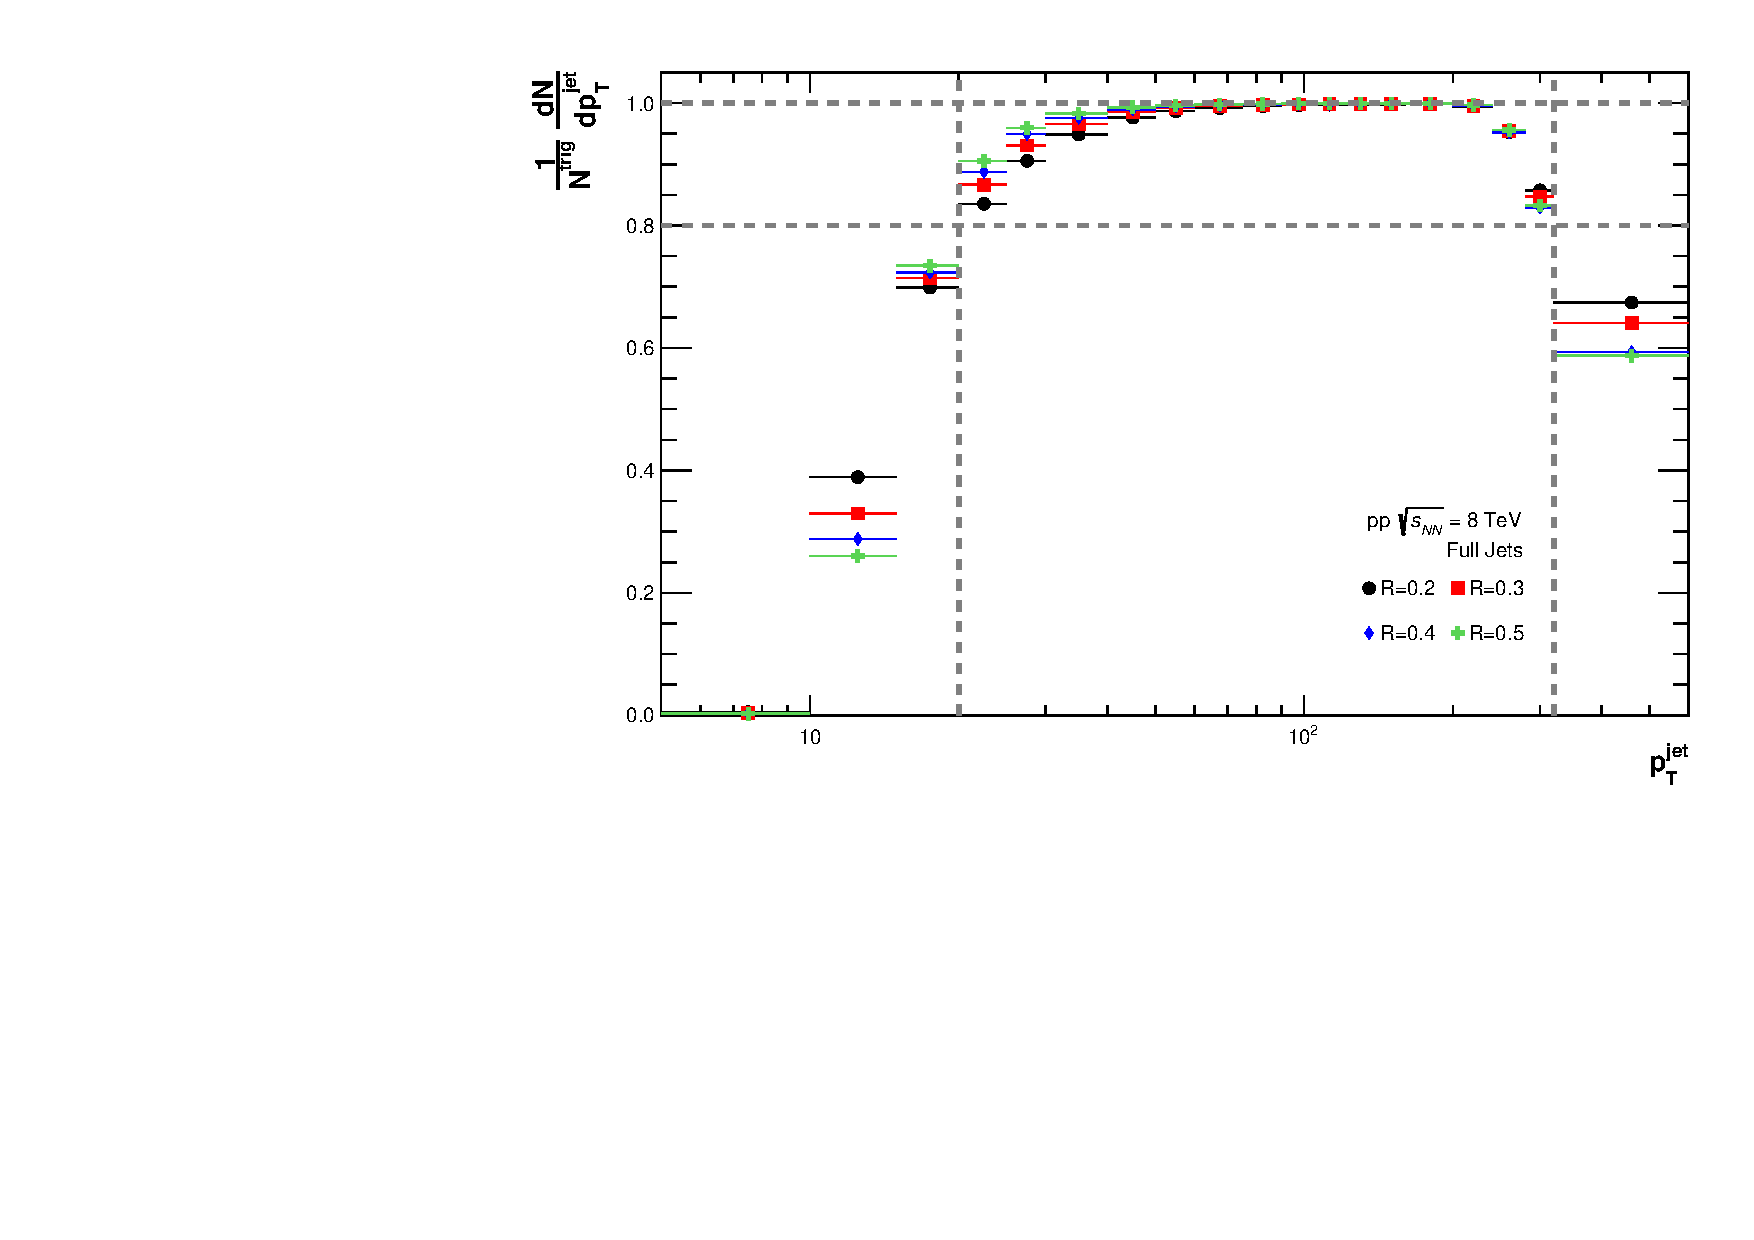
\includegraphics[width=15cm]{figures/KinematicEfficiency/EffKine.pdf}
    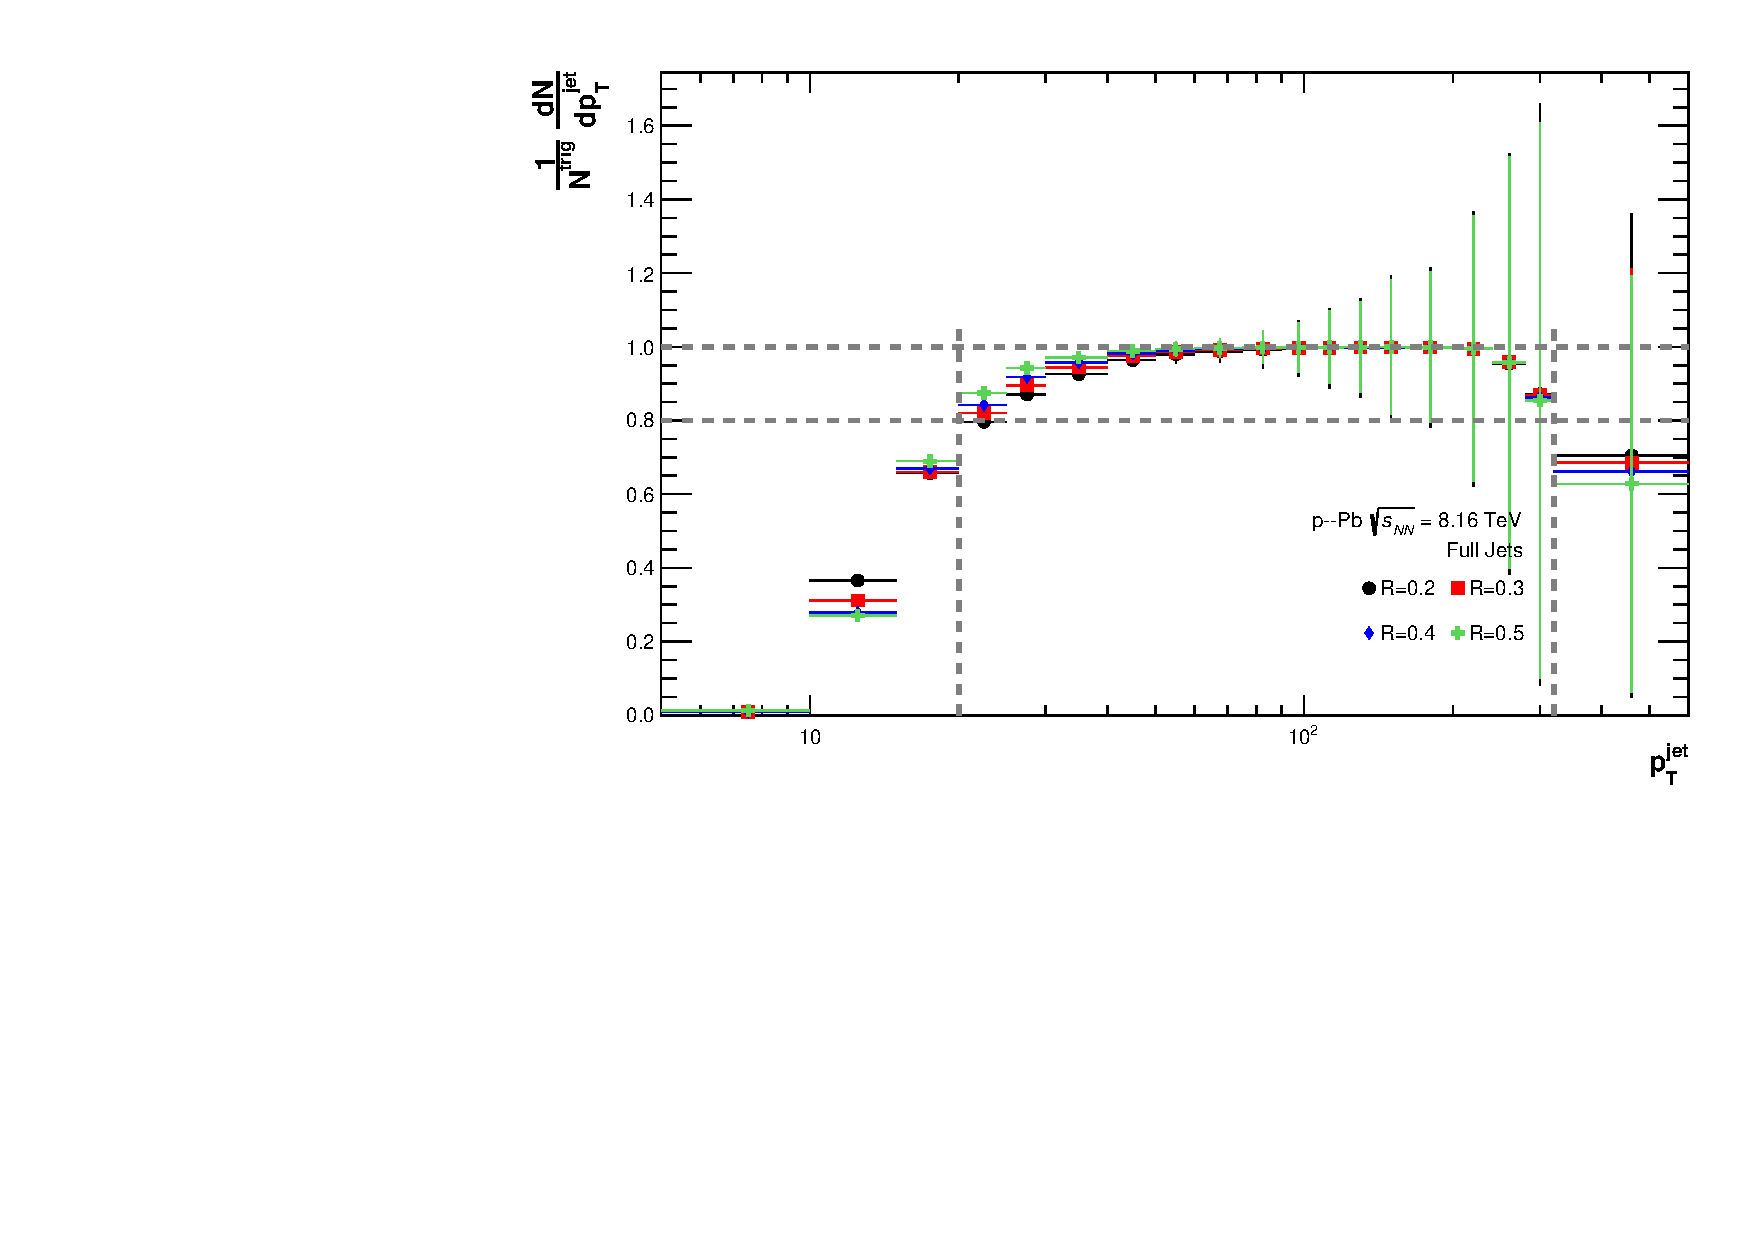
\includegraphics[width=15cm]{figures/pPbFigures/KinematicEfficiency/EffKine.pdf}
    \caption{Kinematic efficiency for various jet radii in \pp (top) and \pPb (bottom).}
    \label{fig:KinematicEfficiency}
\end{figure}

The kinematic efficiency is the fraction of particle level jets matched to jets which are reconstructed at detector level. Truncating the response matrix at low and high \pT at detector level causes some jets at particle level to be lost because they fall outside the chosen range. By dividing by the kinematic efficiency, the spectrum is corrected for jets that were reconstructed but did not pass the matching criteria, i.e. jets that were not matched between particle and detector level because they fell outside the selected \pT range or detector acceptance. The kinematic efficiency is found by taking a projection of the response matrix over the selected detector range relative to the full range. The kinematic efficiency must be at least 80$\%$ in order to ensure each bin is well constrained by data. Low percentages suggest that the jets in that kinematic range would need to be heavily corrected by unfolding and are thus highly dependent on PYTHIA. The choice of 80$\%$ was determined by ALICE to be within a range that is constrained sufficiently by data.

Figure~\ref{fig:KinematicEfficiency} shows the kinematic efficiency for jets with R = 0.2 to R = 0.6 for \pp and R = 0.2 to R = 0.5 for \pPb. Jets are selected at detector level to have a \pT within 10 and 240 GeV/$c$. The efficiency is 80$\%$ beyond 20 GeV/$c$, and stays around this value in the whole region covered by the measurement. At lower \pT, the turn-on is sharper for jets with larger jet radii. A measurement is feasible for 20 GeV /c $<$ \pT $<$ 320 GeV/$c$ where the kinematic efficiency is larger than 80$\%$.

\subsection{Unfolding of the jet spectrum}
\label{sec:unfolding}

For this measurement, both Bayesian unfolding and unfolding based on singular value decomposition (SVD) are used to correct the spectrum. Both methods were implemented in the RooUnfold framework \cite{roounfold}. The Bayesian method is used as the standard method, while SVD unfolding is used to test the sensitivity with respect to different unfolding methods. The unfolding process must be dealt with carefully due to several assumptions made. First, it is assumed that the true spectrum has a similar shape to the Monte Carlo spectrum used to create the detector response. Second, the assumption is made that a jet reconstructed at detector level corresponds to a jet reconstructed at truth level. These assumptions can lead to biases in the results. Several tests are performed to minimize the impact of these biases on the final spectrum.

Bayesian unfolding, introduced by D'Agostini~\cite{D'Agostini:265717}, is an iterative process to find the best estimate for true spectrum from the raw spectrum. The raw spectrum refers to the jet spectrum after scaling correction but before unfolding, as in Equation~\ref{eq:corrraweq}. This process can be expressed in terms of causes C, representing the true spectrum, and effects E, representing the raw spectrum. Each cause can impact multiple effects, and the exact cause for a given effect is not known. Bayes theorem is then given by the equation

\begin{equation}
    P(C_i|E_j) = \frac{P(E_j|C_i)\cdot P_0(C_i)}{\Sigma_l^{n_C}P(E_j|C_l)\cdot P_0(C_l)}
\end{equation}

\noindent
where $P(C_i|E_j)$ is the probability that a cause is responsible for a specific effect, $P(E_j|C_i)$ is the probability of having an effect produced from a defined cause, and $P_0(C_i)$ is the prior or initial probability of causes. $P(E_j|C_i)$ can also be thought of as the distribution of migration probabilities, or the probability of a cause migrating to a given effect. This can be thought of as a jet of a certain true momentum being reconstructed at some other momentum. The expected number of events for a given cause representing the true spectrum is then given by

\begin{equation}
    \hat{n}(C_i) = \frac{1}{\epsilon_i}\Sigma_{j=1}^{n_E}n(E_j)\cdot P(C_i|E_j), \; \epsilon_i \neq 0
\end{equation}

\noindent
where $\epsilon_i$ is the efficiency of a cause producing an effect, and $n(E_j)$ is the number of events for a given effect representing the measured or smeared spectrum. This equation can be rewritten in terms of the response matrix as

\begin{equation}
    \hat{n}(C_i) = \Sigma_{j=1}^{n_E}M_{ij}\cdot n(E_j)
\end{equation}

\noindent
where the response matrix is

\begin{equation}
    M_{ij} = \frac{P(E_j|C_i)\cdot P_0(C_i)}{[\Sigma_{l=1}^{n_E}P(E_l|C_i)] \cdot [\Sigma_{l=1}^{n_C}P(E_j|C_l)\cdot P_0(C_l)]}
\end{equation}

\noindent
Due to the iterative nature of the Bayesian process, a perfect prior knowledge of the behavior of the true spectrum is not required. The prior can be chosen to be flat or uniform, and a satisfactory result can still be reached. The prior is typically taken from Monte Carlo simulations and is taken from PYTHIA in this instance because it gets most aspects of the spectrum correct. The closer the prior is to the true spectrum, the better the outcome will be. To iterate using the Bayesian process, the prior is replaced by the new "true" spectrum, and the process is repeated until the spectrum converges. 

Unfolding using the SVD method was first introduced by Hocker and Kartvelishvili~\cite{Hocker:1995kb}. This method again begins with the relationship between the true spectrum x and the raw spectrum b, given by

\begin{equation}
    \hat{A}x = b
\end{equation}

\noindent
where $\hat{A}$ is the response matrix. The response matrix is then decomposed into three matrices, $U$, $S$, and $V$ as 

\begin{equation}
    \hat{A} = U \cdot S \cdot V^T
\end{equation}

\noindent 
where U is an $m \times m$ orthogonal matrix, V is an $n \times n$ orthogonal matrix, and S is an $m \times n$ diagonal matrix of singular values. By swapping rows of the orthogonal matrices, the singular values can be ordered from largest to smallest. The inverse of the response matrix is easier to perform on the decomposed matrix, since S is diagonal, and the inverse of an orthogonal matrix is its transpose. The original system is 

\begin{equation}
    USV^Tx = b
\end{equation}

\noindent
Introducing vectors $z = V^Tx$ and $d = U^Tb$, the solution is given by

\begin{equation}
    z_i = \frac{d_i}{s_i}, \; x = Vz
\end{equation}

\noindent 
Two issues can arise with this solution. The first is that the singular values can be very small or zero, which can lead to large fluctuations in the solution. The second is that $d_i$ can be poorly known or insignificant. Inspecting the exact solution $z_i$ as a function of $|d_i|$, also known as the D-vector, shows that at high enough i values of $|d_i|$, changes to the solution are insignificant. A regularization parameter $k$ is introduced to the solution in the form 

\begin{equation}
    z_i^{(k)} = \frac{d_i}{s_i}\cdot \frac{s_i^2}{s_i^2 + s_k^2}
\end{equation}

\noindent
where k should be chosen to be the index of the last significant d. If k is chosen to be too small, the solution will be dominated by the prior. If it is too large, the solution will be dominated by high frequency statistical fluctuations.

The following figures contain unfolding test results for jet resolution parameter R = 0.2 for SVD and Bayesian unfolding to ensure stability of the unfolding process (for the remaining jet radii, see Appendix~\ref{sec:AppendixUnfoldingTests}). The goal of performing these tests is to find convergence of the jet spectra with increasing regularizations or iterations of the unfolding procedure.


\begin{figure}[hbt!]
    \centering
    \begin{multicols}{2}
            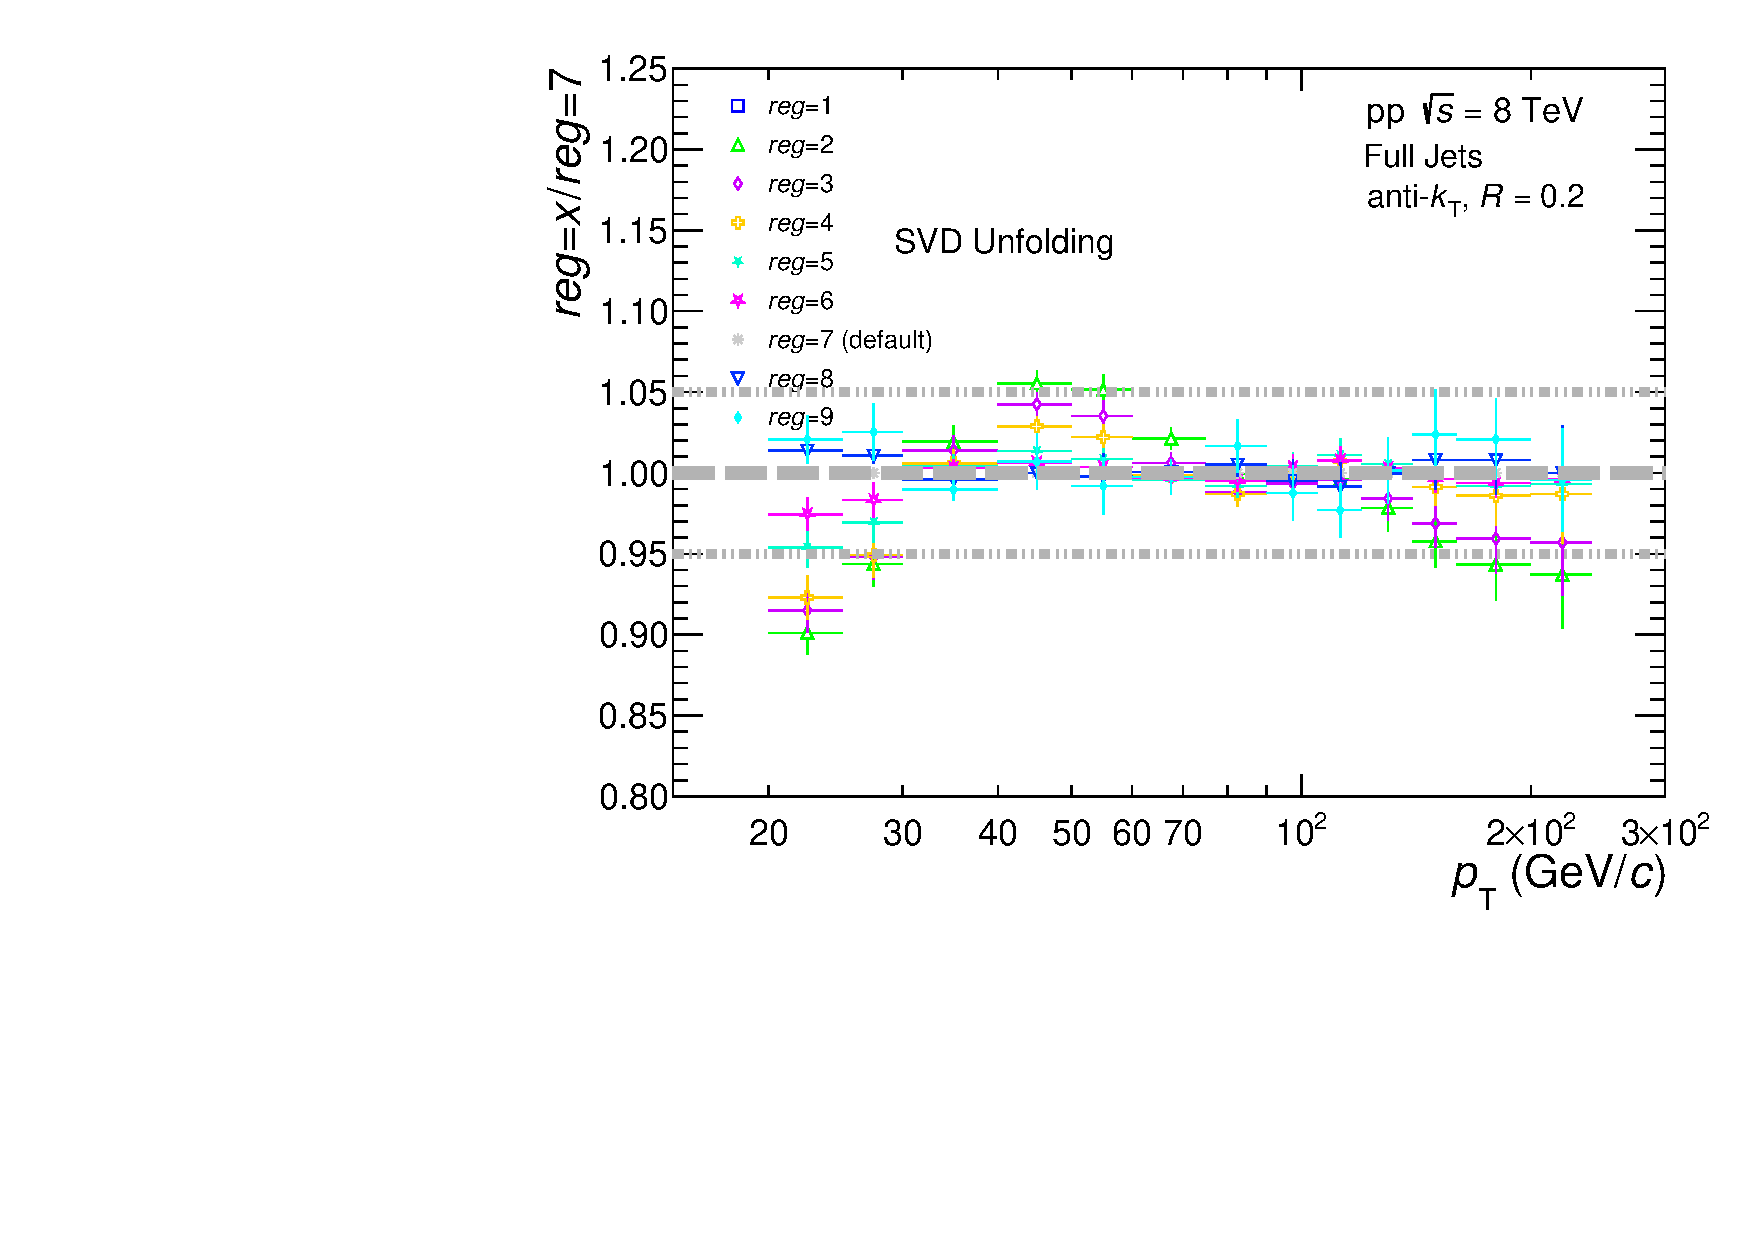
\includegraphics[width=0.49\textwidth]{figures/UnfoldingComparisons/Regularizations/RatioRegularizationSvd_R02.pdf}
        \vfill\null 
        \columnbreak
            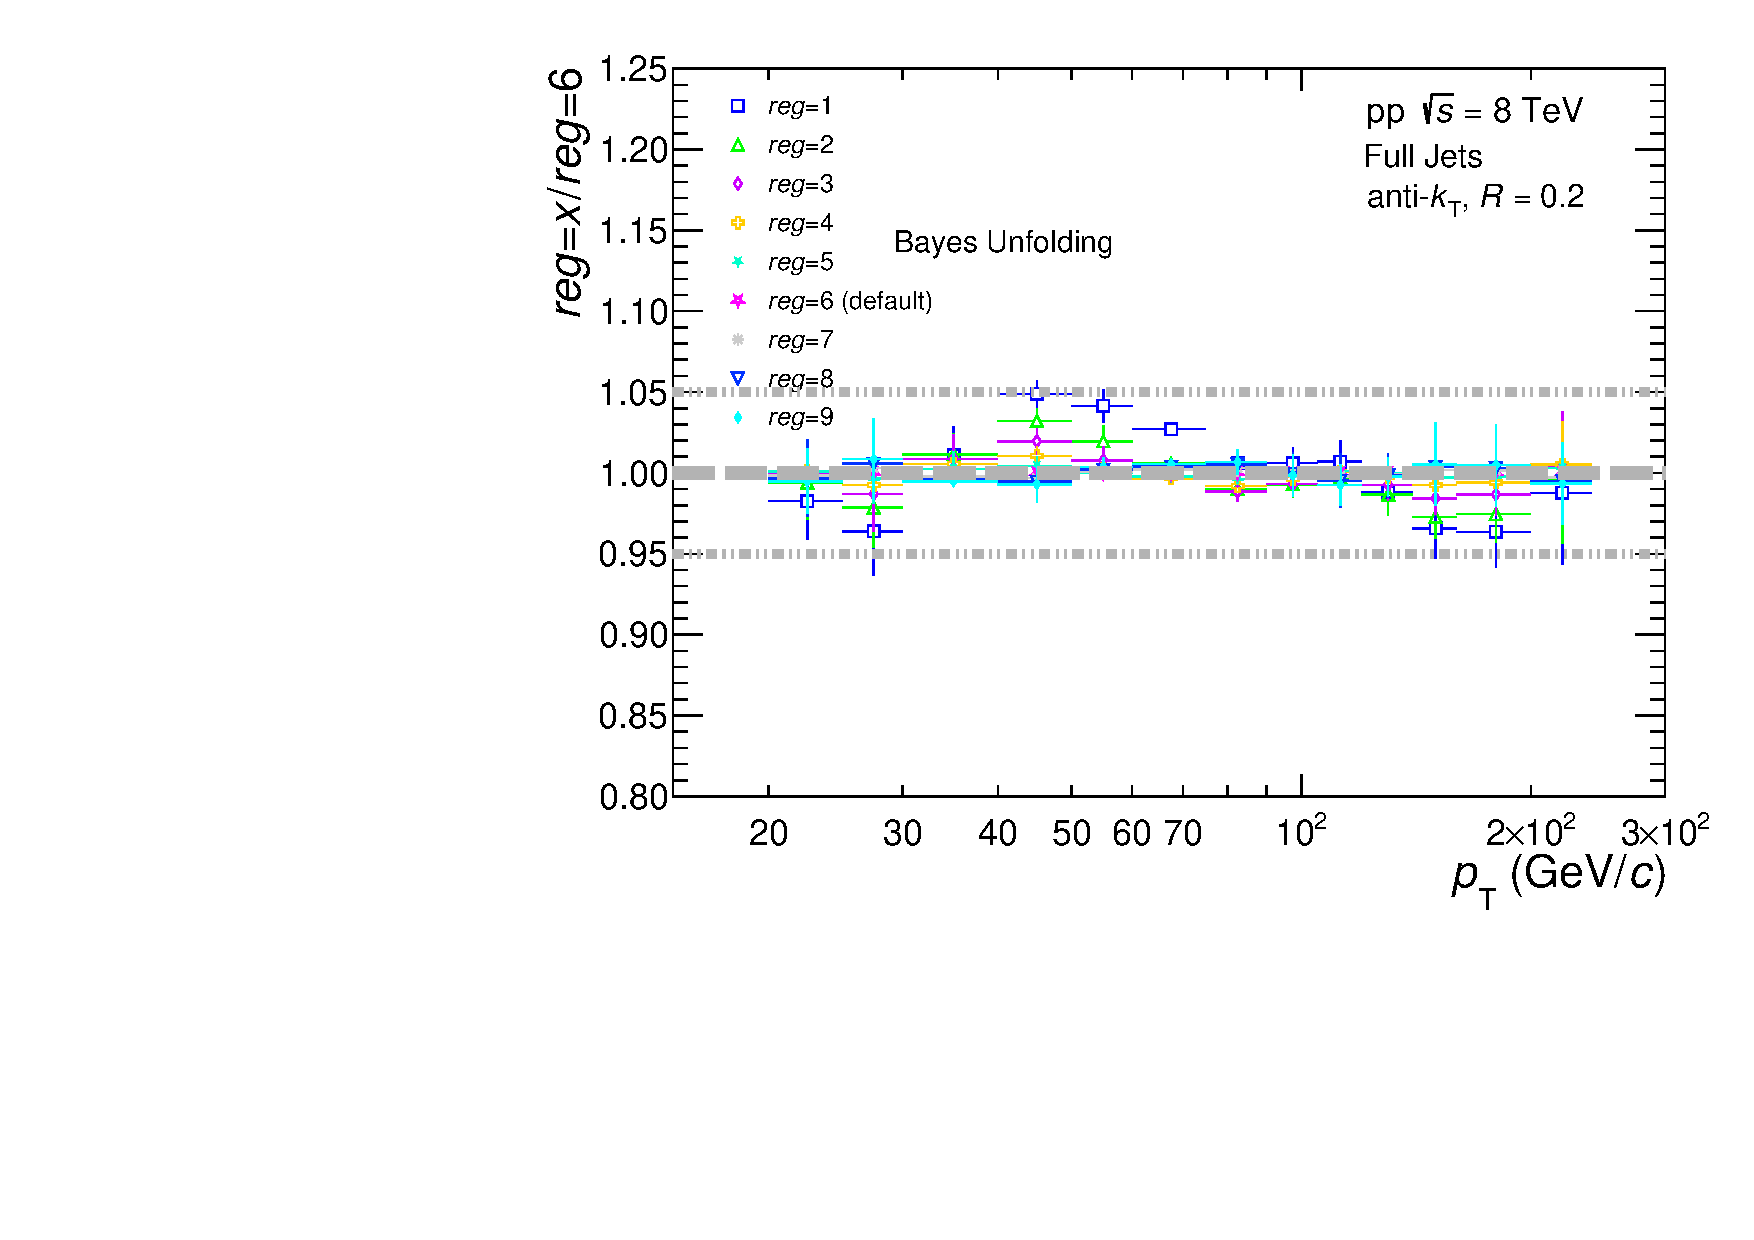
\includegraphics[width=0.49\textwidth]{figures/UnfoldingComparisons/Regularizations/RatioRegularizationBayes_R02.pdf}
        \vfill\null
    \end{multicols}
    \caption{Regularization dependence for SVD (left) and iterations of Bayesian (right) unfolding of jets in \pp collisions. Iterations are also labeled as "reg" in this plot for visual comparison between the methods.}
    \label{fig:RegIter}
\end{figure}


Figure~\ref{fig:RegIter} shows the dependence of the SVD and Bayesian unfolded solutions on the regularization parameter and number of iterations, respectively. A regularization parameter of 7 is selected as default for the SVD unfolding, while 6 iterations are chosen as default for Bayesian unfolding with 4 and 9 iterations as variations. The choice of the regularization parameter for SVD of 7 is also motivated by the D-vector, shown in Figure~\ref{fig:DVector}. At low values of regularization parameter, the D-vector falls steeply. Changes in this regime are statistically significant. When the D-vector reaches a plateau, the spectrum no longer changes significantly with further regularizations. The default solution is chosen in this region. With increasing regularizations or number of iterations, the spectrum must at some point no longer change significantly and converge on a default solution.


\begin{figure}[hbt!]
    \centering
    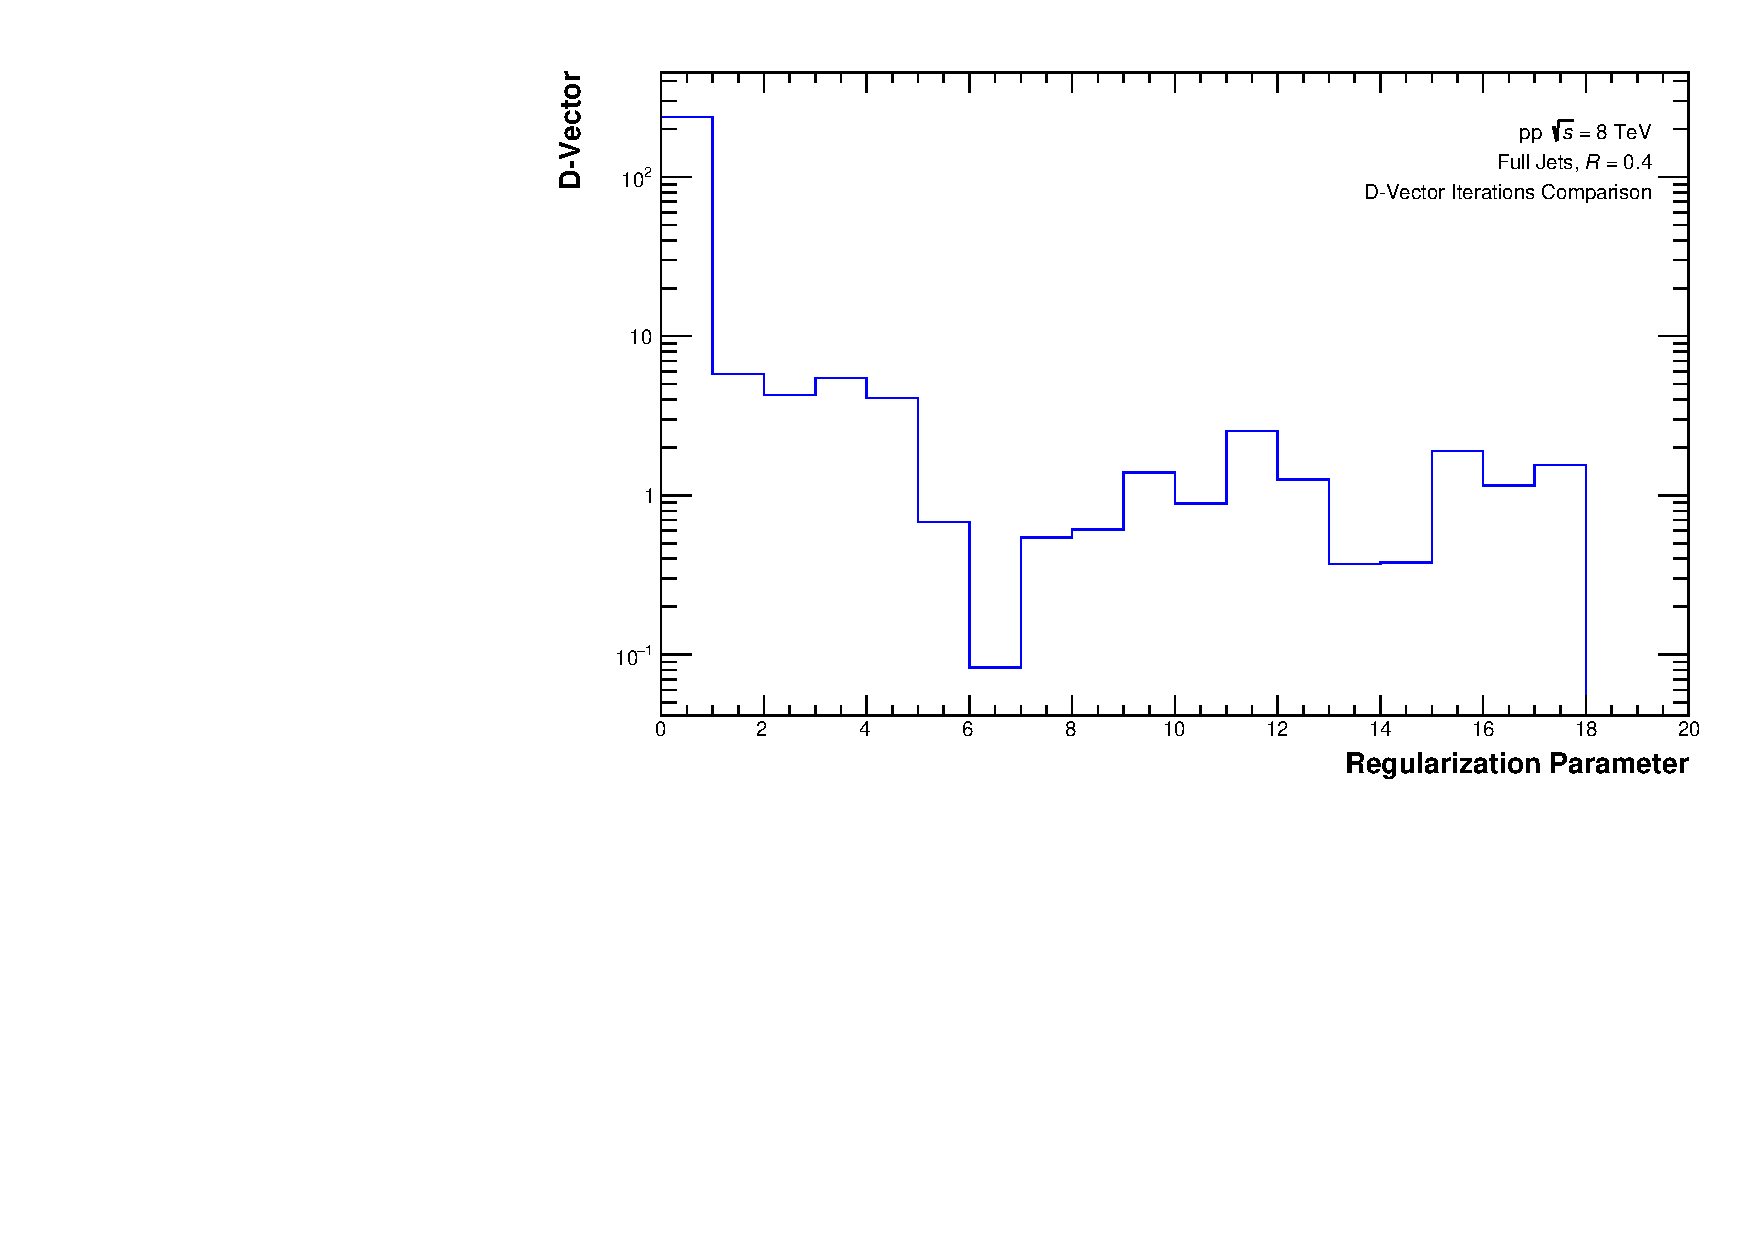
\includegraphics[width=15cm]{figures/DVector/DVector_R04.pdf}
    \caption{D-Vector comparison for multiple regularizations of SVD unfolding of the jet spectrum for $R$ = 0.4 in \pp collisions.}
    \label{fig:DVector}
\end{figure}


\begin{figure}[hbt!]
    \centering
    \begin{multicols}{2}
        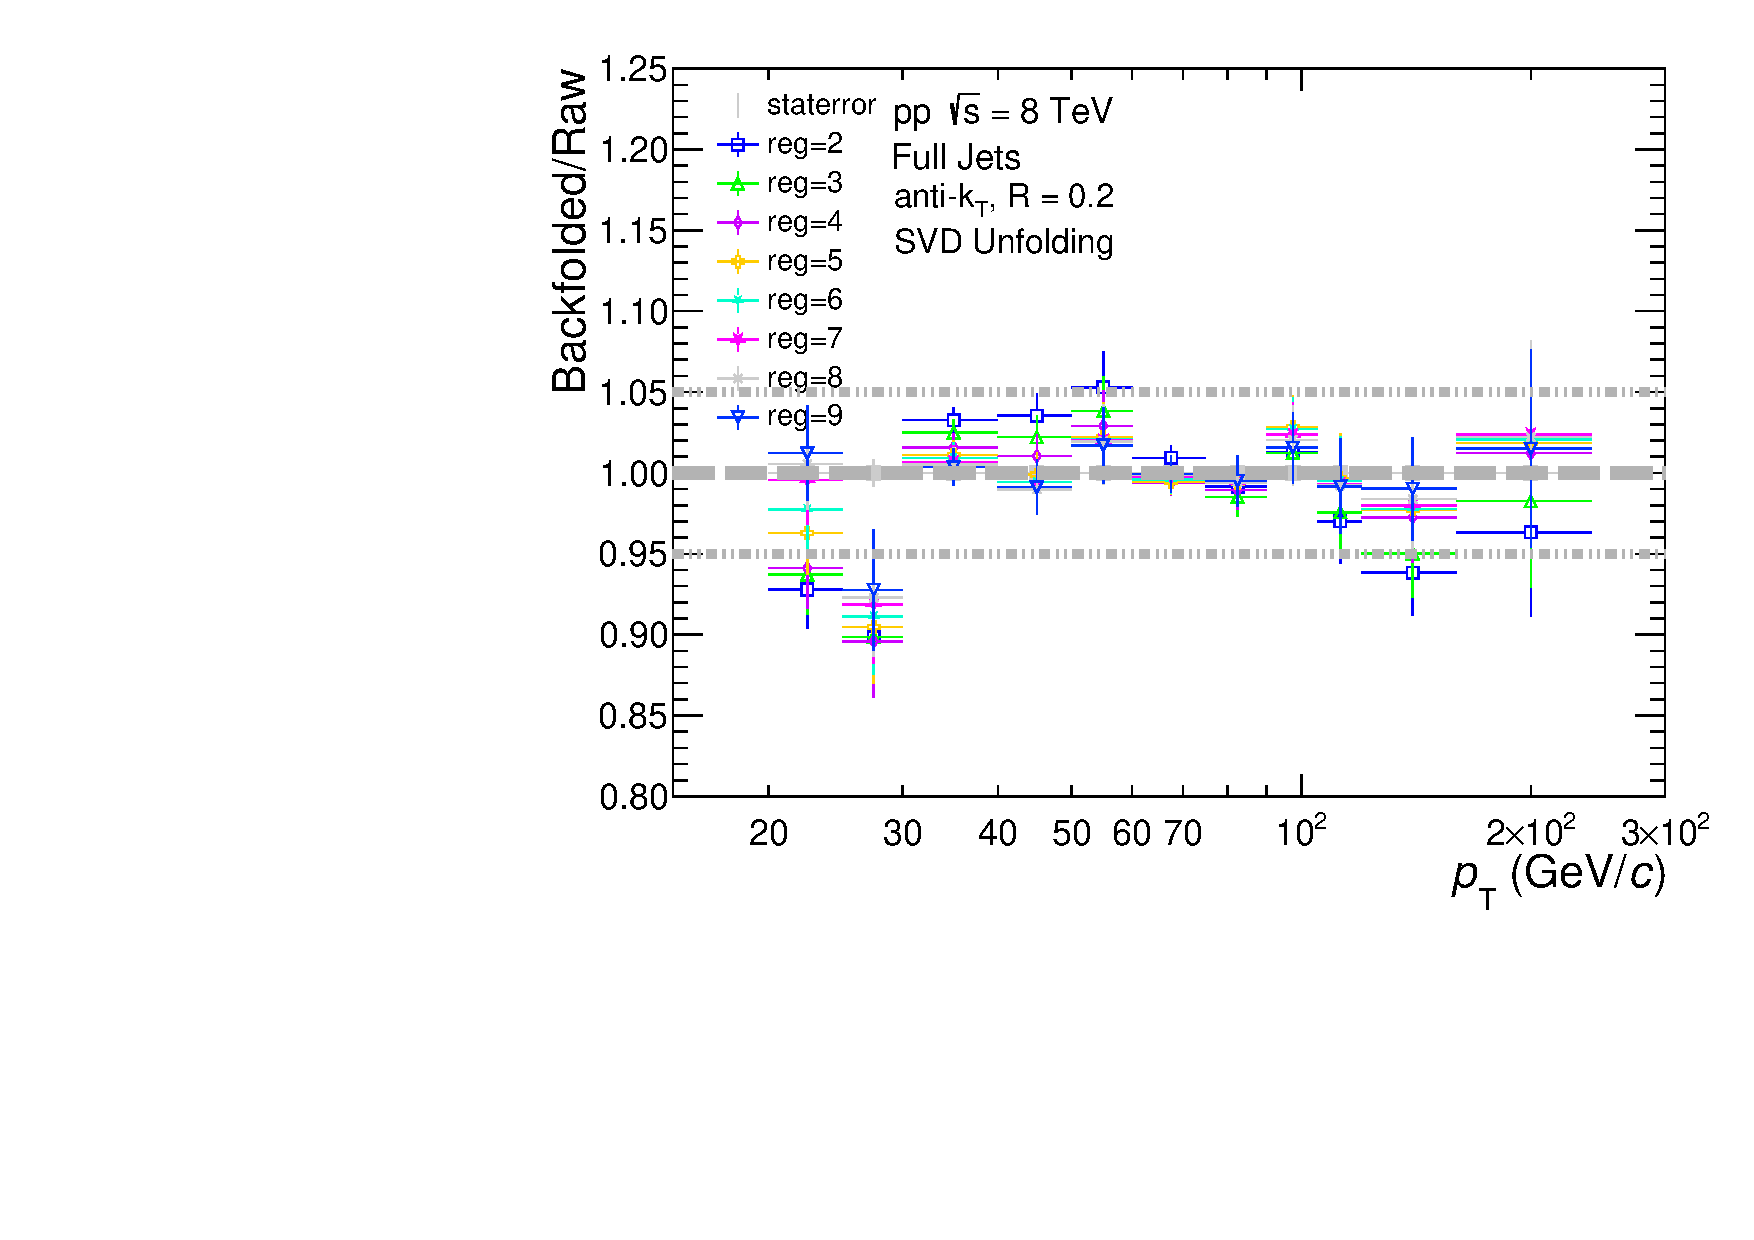
\includegraphics[width=0.49\textwidth]{figures/UnfoldingComparisons/BackfoldedVsRaw/RatioFoldRawSvd_R02.pdf}
    \vfill\null
    \columnbreak
        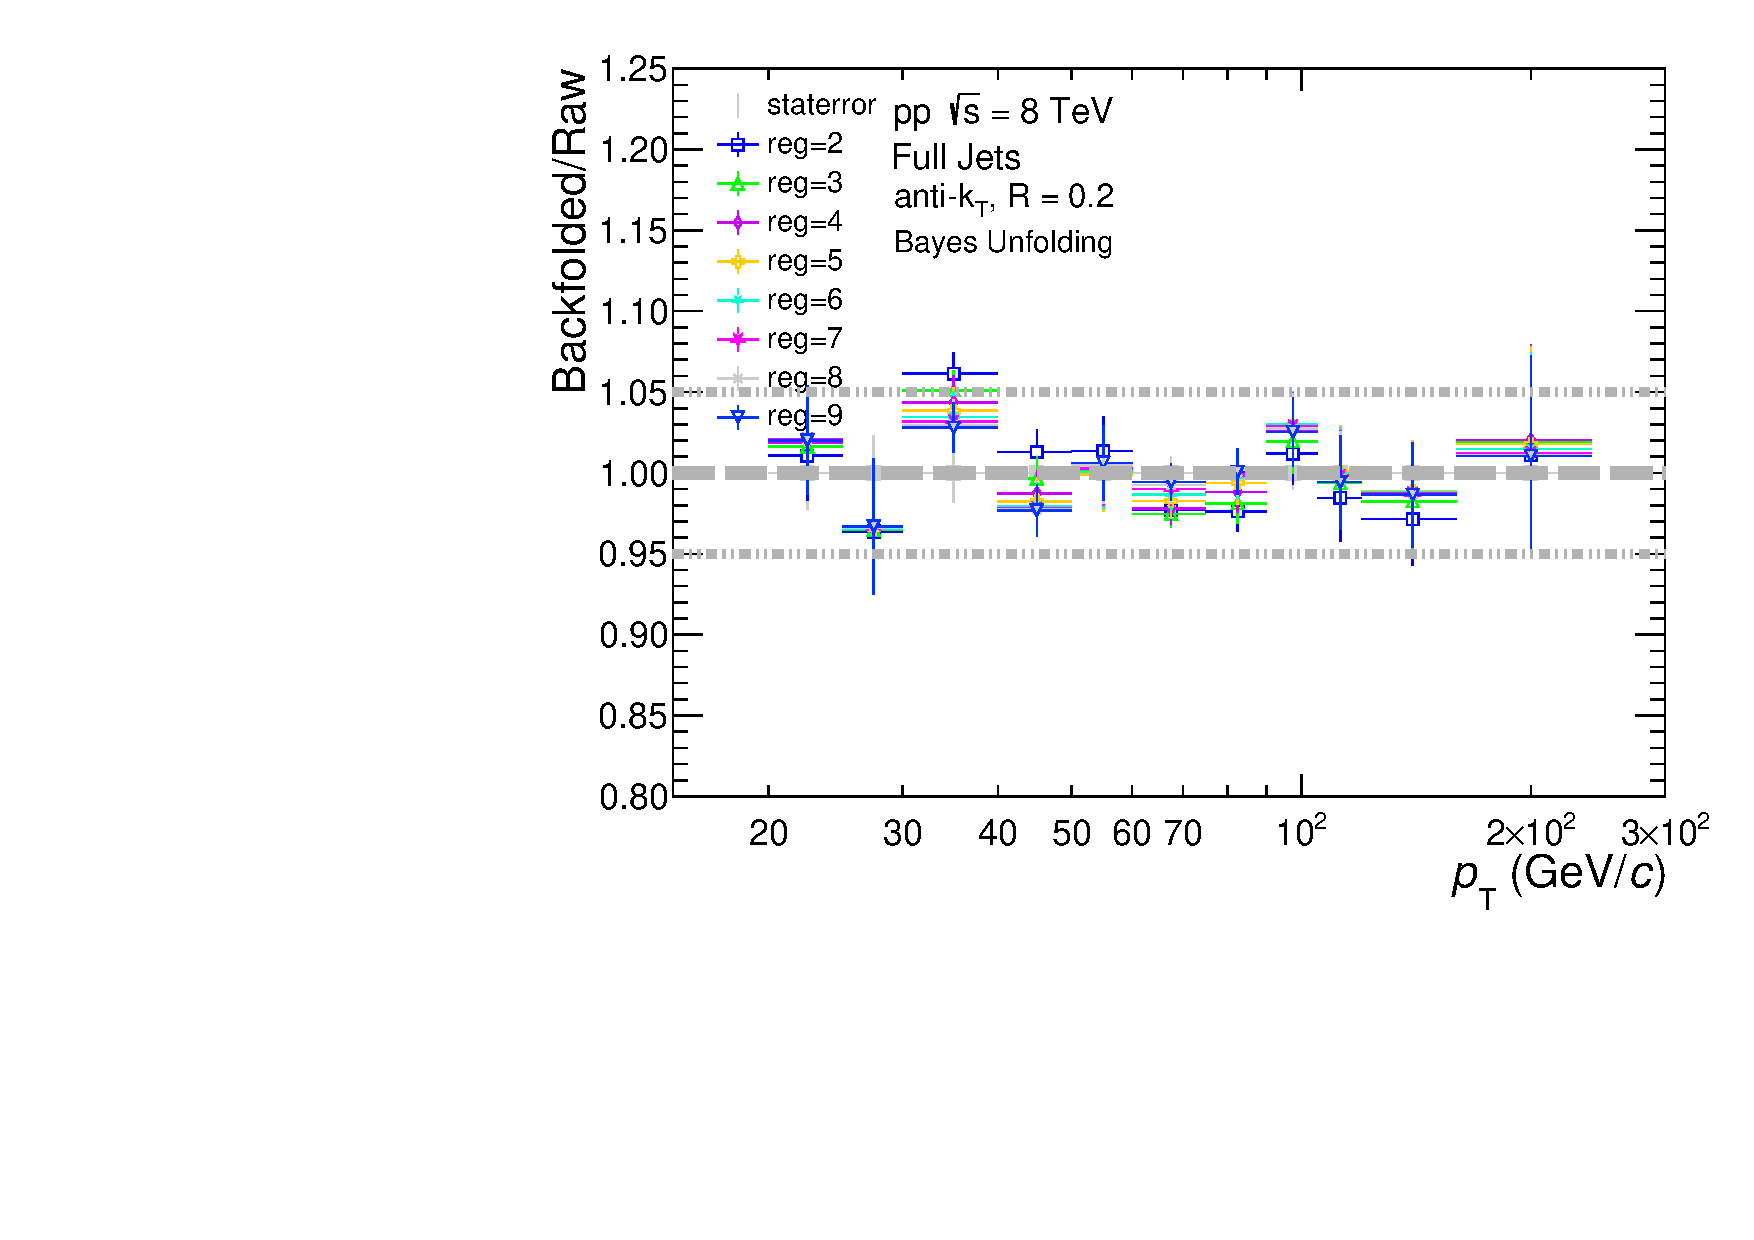
\includegraphics[width=0.49\textwidth]{figures/UnfoldingComparisons/BackfoldedVsRaw/RatioFoldRawBayes_R02.pdf}
        \vfill\null
    \end{multicols}
    \caption{Backfolded spectrum for multiple iterations vs. the raw spectrum for R=0.2 in jets from \pp collisions.}
    \label{fig:BackfoldedRaw}
\end{figure}


Figure~\ref{fig:BackfoldedRaw} shows the comparison of the backfolded spectrum to the uncorrected spectrum for several regularizations for SVD and Bayesian unfolding. This test attempts to re-fold the results by re-applying the response matrix to undo the original process and makes a comparison to the original raw spectrum. The backfolded spectrum should ideally match the raw spectrum as closely as possible.


\begin{figure}[hbt!]
    \centering
    \begin{multicols}{2}
            \includegraphics[width=0.49\textwidth]{figures/UnfoldingComparisons/Closure/RatioClosure1DSvd_R02.pdf}
        \vfill\null
        \columnbreak
            \includegraphics[width=0.49\textwidth]{figures/UnfoldingComparisons/Closure/RatioClosure1DBayes_R02.pdf}
        \vfill\null
    \end{multicols}
    \caption{Closure test for the unfolding of jet resolution parameter R=0.2 in jets from \pp collisions.}
    \label{fig:Closure}
\end{figure}


Figure~\ref{fig:Closure} shows the Monte Carlo closure test for SVD and Bayesian unfolding, where the Monte Carlo sample is split randomly with 20$\%$ used for the smeared spectrum and 80$\%$ used for the response matrix. The test shows agreement between the true spectrum and the unfolded solution.

The same unfolding tests were performed to check the stability of the unfolding process for jets reconstructed in the \pPb dataset. Figure~\ref{fig:RegIterpPb} shows the ratio of the spectra for several regularizations or iterations to the chosen default solution. Convergence is not achieved as quickly as in \pp collisions, but the solution stabilizes with increasing iterations or regularizations. Convergence is not reached as quickly due to low statistics in the trigger transition region causing unfolding instabilities. Figure~\ref{fig:BackfoldedRawpPb} shows the comparison of the backfolded to the raw spectrum. Just as in \pp collisions, the final bins have large uncertainties with central points lying further from unity, but the solution still converges on itself with increasing iterations or regularizations. Figure~\ref{fig:ClosurepPb} shows the Monte Carlo closure tests, which show good convergence at unity within very few iterations or regularizations. Figure~\ref{fig:DVectorpPb} shows the D-vector analysis, which reaches a plateau in a similar range to \pp collisions. All tests show convergence in final \pT range reported. Appendix~\ref{sec:AppendixUnfoldingTestspPb} contains the remaining jet radii.


\begin{figure}[hbt!]
    \centering
    \begin{multicols}{2}
            \includegraphics[width=0.49\textwidth]{figures/pPbFigures/UnfoldingComparisons/Regularizations/RatioRegularizationSvd_R02.pdf}
        \vfill\null 
        \columnbreak
            \includegraphics[width=0.49\textwidth]{figures/pPbFigures/UnfoldingComparisons/Regularizations/RatioRegularizationBayes_R02.pdf}
        \vfill\null
    \end{multicols}
    \caption{Regularization dependence for SVD (left) and Bayesian (right) unfolding of jets in \pPb collisions. Iterations are also labeled as "reg" in this plot for visual comparison between the methods.}
    \label{fig:RegIterpPb}
\end{figure}



\begin{figure}[hbt!]
    \centering
    \begin{multicols}{2}
        \includegraphics[width=0.49\textwidth]{figures/pPbFigures/UnfoldingComparisons/BackfoldedVsRaw/RatioFoldRawSvd_R02.pdf}
    \vfill\null
    \columnbreak
        \includegraphics[width=0.49\textwidth]{figures/pPbFigures/UnfoldingComparisons/BackfoldedVsRaw/RatioFoldRawBayes_R02.pdf}
        \vfill\null
    \end{multicols}
    \caption{Backfolded spectrum for multiple iterations vs. the raw spectrum for R=0.2 in jets from \pPb collisions.}
    \label{fig:BackfoldedRawpPb}
\end{figure}



\begin{figure}[hbt!]
    \centering
    \begin{multicols}{2}
            \includegraphics[width=0.49\textwidth]{figures/pPbFigures/UnfoldingComparisons/Closure/RatioClosure1DSvd_R02.pdf}
        \vfill\null
        \columnbreak
            \includegraphics[width=0.49\textwidth]{figures/pPbFigures/UnfoldingComparisons/Closure/RatioClosure1DBayes_R02.pdf}
        \vfill\null
    \end{multicols}
    \caption{Closure test for the unfolding of jet resolution parameter R=0.2 in jets from \pPb collisions.}
    \label{fig:ClosurepPb}
\end{figure}


\begin{figure}[hbt!]
    \centering
    \includegraphics[width=15cm]{figures/pPbFigures/DVector/DVector_R02.pdf}
    \caption{D-Vector comparison for multiple regularizations of SVD unfolding of the jet spectrum for $R$ = 0.2 jets in \pPb collisions.}
    \label{fig:DVectorpPb}
\end{figure}

\section{Systematic Uncertainties}
\label{ch:Systematics}

\subsection{Spectra}
\label{sec:SystematicsSpectra}

Each contribution to the systematic uncertainty includes one or more variations that are considered for this analysis. The analysis is repeated from start to finish for each variation. The analysis uses ratios for each variation to the default solution for a given contribution and plots them together for review. Five contributions to the unfolding uncertainty are evaluated together in the same manner. For the majority of the contributions to the systematic uncertainty, the mean of the absolute value of the deviations to the default solution is determined for each \pT bin. For the contributions from unfolding, the maximum is used instead of the mean. In order to suppress nonphysical statistical fluctuations, most contributions are fitted with a polynomial, and the value of this fit at each bin center is taken as the true systematic uncertainty. Some contributions are evaluated without fitting, where the uncertainty is not expected to follow a clear pattern. All the uncertainties are then added in quadrature for each bin. All following contributions were considered for both \pp and \pPb collisions, unless otherwise stated. The section titles denote the uncertainties that were considered for only a single system.

\subsubsection{Tracking Efficiency}

The largest contribution to the systematic uncertainty at about 6--10$\%$ is the precision of the tracking efficiency, which is the probability of reconstructing a charged particle that passed through the detector, and primarily affects the scale of the spectrum. The uncertainty on the tracking efficiency was determined to be 4\% for the \pp dataset and 3\% for the \pPb dataset. The higher precision for the \pPb dataset is due to improved spacetime distortion corrections during run 2 as well as better performance of the ITS. The aforementioned "holes" in the SPD were not present during run 2. While the tracking efficiency uncertainty does change with momentum, most tracks within jets fall in a \pT range where the efficiency and the uncertainty on the efficiency are approximately constant~\cite{ALICE:2014sbx}. This quantity is varied by randomly discarding 4\% of Monte Carlo tracks in \pp and 3\% of Monte Carlo tracks in \pPb at detector level before jet finding and construction of the response matrix.

\subsubsection{Unfolding}

The second largest contribution arises from the combined unfolding uncertainties. This contribution is about 2--3$\%$ in \pp and about 5$\%$ for the majority of \pPb, other than where the transition between triggers occurs. These contributions primarily affect the shape of the spectrum. These contributions are as follows: 

\begin{itemize}
    \item[1)] The number of unfolding iterations is varied with +3/-2 iterations of Bayesian unfolding considered.
    \item[2)] The measured distribution and the response matrix are truncated at different values. The default minimum accepted jet \pT is 10 GeV. As variations, $\pm 5$ GeV are considered.
    \item[3)] The default prior is PYTHIA 8, the Monte Carlo used in the generation of the response. The ratio between the default unfolded solution and the default prior is applied as a weight to the original response matrix as a variation to the prior.
    \item[4)] The way in which the spectrum is binned at detector level causes statistically significant variations in the spectrum from unfolding. To ensure the final spectrum is not highly dependent on the way it is binned, four variations to the binning of the spectrum before unfolding are considered.
    \item[5)] Bayesian unfolding is used by default with SVD as a variation. The difference between the Bayesian and the SVD method is primarily used in order to account for the discrepancy seen between the two methods in the region where the triggers swap.
\end{itemize}

\subsubsection{EMCal Seed and Cell Thresholds}

The EMCal seed threshold is the lowest energy required for a signal in the EMCal to be considered for clusterization. The clusterization process adds all adjacent cells that are above the cell threshold to the cluster. The variations to the seed and cell thresholds are found in Table~\ref{tab:SeedCellThresholds}.


\begin{table}[hbt!]
    \centering
    \caption{Seed and cell threshold systematic variations for EMCal clustering.}
    \begin{tabular}{ | m{1.7cm} | m{4.1cm}| m{4.1cm} | } 
      \hline
      Variation & Seed Threshold (MeV) & Cell Threshold (MeV) \\
      \hline
      Default & 300 & 100 \\ 
      \hline
      Low & 275 & 75 \\ 
      \hline
      High & 350 & 100 \\ 
      \hline
    \end{tabular}
    \label{tab:SeedCellThresholds}
\end{table}

\subsubsection{Clusterizer Algorithm}

The default clusterizer algorithm used to cluster towers that pass the seed and cell thresholds in the EMCal is the "Clusterizer v3" algorithm. The NxN clusterizer with N = 3 and N = 5 are considered as variations, where N is the number of EMCal towers.

\subsubsection{Hadronic Correction}

The energy of clusters in the EMCal is corrected for the hadronic contribution. Since tracks are used in the analysis, the contribution from hadrons which leave deposits in the calorimeter must be subtracted off to avoid double counting the energy. By default, the momentum of the track in the ITS+TPC is fully subtracted from the cluster. While standard for jet analyses in ALICE, this is an extreme assumption, presuming that all tracks are electrons. The EMCal is not designed to measure the full hadronic energy due to its short hadronic interaction length, so hadrons interacting with the calorimeter material only leave partial showers. For this reason, the full subtraction of all tracks may lead to an over-correction for the hadronic energy. Two variations are considered. In one case, 70\% of the momentum of the matched tracks is subtracted. In the other, the minimally ionizing particle (MIP) energy is subtracted, which is 235.6 MeV in data and 282.4 MeV in Monte Carlo.

\subsubsection{Trigger Rejection Factor (\pp only)}

In \pp collisions, the trigger rejection factor is used to correct the downscaling of the spectra from different triggers. The rejection factor is calculated by linearly fitting to the ratio of triggers at the plateau after the turn-on. The cluster spectra are corrected for the cluster trigger efficiency. By default, this fit starts at 4 GeV for the lower trigger and 12.25 GeV for the higher trigger. Variations of $\pm 0.5$ GeV are considered. To account for the uncertainty on the rejection factor, the uncertainty extracted from these variations is combined with the uncertainty of the fit.

\subsubsection{Trigger Transition Threshold}

In order to combine the spectra from different triggers, a transition must occur from one trigger to the next once the higher threshold trigger reaches maximum efficiency. By default, the transition from the INT7 trigger to the EMC7 trigger in \pp collisions occurs at 30 GeV/$c$ of jet momentum, and the transition from the EMC7 trigger to the EJE trigger occurs at 60 GeV/$c$. In \pPb collisions, the transition from the INT7 trigger to the EJ2 trigger again occurs at 30 GeV/$c$, while the transition from the EJ2 trigger to the EJ1 trigger occurs at 60 GeV/$c$. Variations of $\pm 5$ GeV are considered for the transition to the lower threshold EMCal trigger, while variations of $\pm 10$ GeV are considered for the transition to the higher threshold EMCal trigger. The largest influences on this variation arise from the limited statistics of the lower threshold trigger with increasing \pT and the decreasing efficiency of the higher threshold trigger with decreasing \pT.

\subsubsection{Maximum Track Momentum and Cluster Energy}

An upper limit is placed on both the track momentum and cluster energy of 200 GeV by default. In this regime, the \pT resolution of charged tracks is significantly worse, so variations are required in order to reduce bias from tracks reconstructed with incorrect momentum. Variations of 125, 150, 175, and 225 GeV are tested. The selected upper range impacts the entire range of the spectra due to effects from unfolding.

\subsubsection{Q/\pT Shift}

The spectrum is varied for the Q/\pT shift caused by space-time distortions in the TPC. These distortions cause a momentum dependent offset in the number of positive and negative tracks which is studied by taking the ratio between the two. By default, no shift is considered. A 0.2$\%$ shift is considered as a variation. This shift was determined by running a PYTHIA8 simulation and applying a shift to the tracks. This analysis chooses the shift that is most closely aligned with data. Figure~\ref{fig:QoverPtShift} shows the comparison of different simulated Q/\pT shift values compared to ALICE data points in black. A linear fit to the simulated points is given for visual clarity.


\begin{figure}[hbt!]
    \centering
    \includegraphics[width=15cm]{figures/QoverPtShift/QPTComparison.pdf}
    \caption{Comparison of different Q/\pT shift values showing the ratio of positive to negative tracks as a function of \pT. Three different simulated shift values are shown along with ALICE data.}
    \label{fig:QoverPtShift}
\end{figure}

\subsubsection{Background Fluctuations (\pPb only)}

Two additional uncertainties need to be considered for jets from \pPb collisions. The first one accounts for the uncertainty in the estimation of the background fluctuations around the average background density $\rho$. As discussed in Chapter~\ref{sec:backgroundSubtraction}, a $\delta$-\pT formed using the random cones method is used by default to smear the response matrix. As a variation, the $\delta$-\pT matrix is instead formed using single-track embedding. In this method, a track is embedded azimuthally perpendicular to the jet axis, where the underlying event is expected to dominate. The resulting momentum smearing is

\begin{equation}
    \delta \text{\pT}_\text{jet}^\text{emb} = \text{\pT}_\text{jet}^\text{raw,emb} - \rho_{\text{CMS}} A_\text{jet} - \text{\pT}^\text{emb}
\end{equation}

\noindent
where $\text{\pT}_\text{jet}^\text{raw,emb}$ is the reconstructed momentum of the jet with the embedded track, $A_\text{jet}$ is the jet area, $\rho_{\text{CMS}}$ is the estimated underlying event \pT density, and $\text{\pT}^\text{emb}$ is the transverse momentum of the embedded track.

\subsubsection{Luminosity (\pPb only)}

Downscaling the luminosity inspected by a trigger is a statistical process with finite precision. This process is needed because events are rejected for downscaling randomly, and there is a difference between the expected (configured) downscaling factor and the observed downscaling factor. In order to propagate the uncertainty on the luminosity into the spectrum, the luminosity is shifted by its corresponding uncertainty for EJ1 and EJ2 separately. The spectrum is scaled by this shifted luminosity, and the unfolded spectrum for each is taken as a variation.

\subsubsection{Total Systematic Uncertainty}

The components of the uncertainty are added in quadrature to obtain the total systematic uncertainty. Treating the uncertainties in this way assumes that they are uncorrelated. For an example, the different components of the systematic uncertainties for R = 0.2 jets in \pp collisions are shown in Figure~\ref{fig:SystematicsSpectraR02}. For other jet radii and individual contributions to the systematic uncertainty, see Appendix~\ref{sec:AppendixSystematics}. The equivalent plot for \pPb is shown in Figure~\ref{fig:SystematicsSpectraR02pPb}, and the equivalent Appendix is~\ref{sec:AppendixSystematicspPb}. In both cases, the uncertainty for nearly all contributions as well as the total systematic uncertainty grows with increasing \pT. The exceptions are the contributions from unfolding, trigger swap momentum variation, and luminosity scaling. These contributions to the uncertainty are largest in the momentum range where the transition between triggers occurs and the spectrum is most sensitive to the unfolding procedure. Other than in the \pT range where the triggers swap, the systematic uncertainty is comparable between the \pp and \pPb datasets with the lowest \pT point falling around 6--7\% uncertainty and the highest \pT point falling around 10--12\% uncertainty for $R$ = 0.2 jets. For both \pp and \pPb, the uncertainty grows with increasing jet resolution parameter, reaching approximately 10\% in the lowest \pT bins and approximately 14\% in the highest \pT bins for the largest jet radii studied. The uncertainties in the trigger transition region are more pronounced for \pPb collisions, reaching over 25\% for the largest radii studied.


\begin{figure}[hbt!]
    \centering
    \includegraphics[width=15cm]{figures/Systematics/TotalSystematics_R02.pdf}
    \caption{All sources of systematic uncertainties in the jet spectrum, including the total systematic uncertainty with all components added in quadrature for $R$ = 0.2 jets in \pp collisions.}
    \label{fig:SystematicsSpectraR02}
\end{figure}

\begin{figure}[hbt!]
    \centering
    \includegraphics[width=15cm]{figures/pPbFigures/Systematics/TotalSystematics_R02.pdf}
    \caption{All sources of systematic uncertainties in the jet spectrum, including the total systematic uncertainty, with all components added in quadrature for $R$ = 0.2 jets in \pPb collisions.}
    \label{fig:SystematicsSpectraR02pPb}
\end{figure}

\subsection{Cross-Section Ratios}
\label{sec:SystematicsRatios}

For the cross-section ratios, the same systematic contributions are considered. With the exception of the trigger rejection factor fit, trigger swap, and unfolding systematic uncertainties, all contributions to the ratio are calculated directly resulting in partial cancellation. The rejection factor fit is not included at all since this contribution cancels entirely. The trigger transition and unfolding contributions for each cross-section in the ratio are added in quadrature to the total uncertainty. Figures~\ref{fig:SystematicsRatiosR02} and~\ref{fig:SystematicsRatiosR02pPb} give examples of the different components of the systematic uncertainties for R = 0.2/0.3 jets in \pp and \pPb collisions, respectively. For other jet radii and individual contributions, see Appendix~\ref{sec:AppendixSystematics} and~\ref{sec:AppendixSystematicspPb} for \pp and \pPb, respectively. In \pp collisions, the same trend is observed with the cross-section ratios. The systematic uncertainty grows with increasing jet \pT and jet resolution parameter. In \pPb collisions, the effect of the error treatment on the unfolding uncertainties is more pronounced. While other contributions partially canceled, the unfolding uncertainty does not. This results in a large uncertainty on the cross-section ratios in the trigger transition region. The larger uncertainty for \pPb collisions results from limited statistics where the INT7 trigger swaps to the EJ2 trigger. In this region, there is minimal overlap where the INT7 trigger runs out of statistics and the EJ2 trigger reaches maximum efficiency.


\begin{figure}[hbt!]
    \centering
    \includegraphics[width=15cm]{figures/Systematics/ratios/TotalSystematics_R02R03.pdf}
    \caption{All sources of systematic uncertainties in the cross-section ratio, including the total systematic uncertainty, with all components added in quadrature for $R$ = 0.2/0.3 jets in \pp collisions.}
    \label{fig:SystematicsRatiosR02}
\end{figure}

\begin{figure}[hbt!]
    \centering
    \includegraphics[width=15cm]{figures/pPbFigures/Systematics/ratios/TotalSystematics_R02R03.pdf}
    \caption{All sources of systematic uncertainties in the cross-section ratio, including the total systematic uncertainty, with all components added in quadrature for $R$ = 0.2/0.3 jets in \pPb collisions.}
    \label{fig:SystematicsRatiosR02pPb}
\end{figure}

\subsection{Nuclear Modification Factor}
\label{sec:systematicsRpA}

The uncertainties for the nuclear modification factor are handled in the same way as the cross-section ratios where the uncertainties are evaluated directly for the ratio and allow for error cancellation. The trigger rejection factor fit does not cancel, and the same is true for the luminosity. The trigger swap and unfolding contributions for each cross-section in the ratio are added in quadrature to the total uncertainty. The uncertainty from background fluctuations is also added in quadrature. The different components of the systematic uncertainties for R = 0.2 jets are shown in Figure~\ref{fig:SystematicsRpPbR02}. For other radii, see Appendix~\ref{sec:AppendixSystematicsRpPb}. The uncertainty is largest in the trigger transition region where the INT7 trigger runs out of statistics before the EJ2 trigger reaches maximum efficiency. As with the jet cross-sections and ratios, the uncertainty grows with increasing jet \pT and jet resolution parameter on average and has a peak in the trigger swap region. For comparison, a summary table of the systematic uncertainties on the \RpPb for charged particle jets at \sNN = 5.02 TeV is given in Table~\ref{tab:chj_sys}. The uncertainties for charged particle jets are generally smaller than for fully reconstructed jets in part due to the additional uncertainties introduced by the EMCal.


%\begin{figure}[hbt!]
%    \centering
%    \includegraphics[width=15cm]{figures/pPbFigures/Systematics/RpPb/TotalSystematics_R02.pdf}
%    \caption{All sources of systematic uncertainties on the nuclear modification factor including the total systematic uncertainty with all components added in quadrature for $R$ = 0.2 jets.}
%    \label{fig:SystematicsRpPbR02}
%\end{figure}

\begin{table}[hbt!]
  \centering
  \caption{Summary of the systematic uncertainties for charged particle jets in \pp and \pPb collisions at 5.02 TeV~\cite{ALICE:2023ama}.}
  \begin{tabular}{  m{2.4cm}  m{4cm} m{4cm}  }
      \hline
      Radius & \pT Range (GeV/$c$) & Sys. Unc. (\%) \\
      \hline
      0.2 & 10--20 & 4.39 \\
          & 120--140 & 9.90 \\
      \hline
      0.3 & 10--20 & 4.83 \\
          & 120--140 & 11.23 \\
      \hline
      0.4 & 10--20 & 6.32 \\
          & 120--140 & 11.22 \\
      \hline
  \end{tabular}
  \label{tab:chj_sys}
\end{table}
\section{Results and Comparison to Simulation}
\label{chap:results}

\subsection{Corrected jet spectrum}
\label{sec:corrJetSpectrum}

\begin{figure}
    \centering
    \includegraphics[width=15cm]{figures/FinalResults/Bayes_reg6.pdf}
    \caption{Jet spectra in \pp for various jet radii after corrections, unfolding, and addition of systematic errors. Scaled for visual clarity.}
    \label{fig:finalSpectra}
\end{figure}

\begin{figure}
    \centering
    \includegraphics[width=15cm]{figures/pPbFigures/FinalResults/Bayes_reg6.pdf}
    \caption{Jet spectra in \pPb for various jet radii after corrections, unfolding, and addition of systematic errors. Scaled for visual clarity.}
    \label{fig:finalSpectrapPb}
\end{figure}

\begin{figure}
    \centering
    \includegraphics[width=15cm]{figures/FinalResults/Bayes_reg6_Ratio.pdf}
    \caption{Jet spectra in \pp for various jet radii compared to R = 0.2 after corrections, unfolding, and addition of systematic errors.}
    \label{fig:finalSpectraRatios}
\end{figure}

\begin{figure}
    \centering
    \includegraphics[width=15cm]{figures/pPbFigures/FinalResults/Bayes_reg6_Ratio.pdf}
    \caption{Jet spectra in \pPb for various jet radii compared to R = 0.2 after corrections, unfolding, and addition of systematic errors.}
    \label{fig:finalSpectraRatiospPb}
\end{figure}

Fig. \ref{fig:finalSpectra} and \ref{fig:finalSpectrapPb} show the comparison of the jet \pT spectra for the different jet radii, while fig. \ref{fig:finalSpectraRatios} and \ref{fig:finalSpectraRatiospPb} show the ratio of R = 0.2 and the remaining radii. Three plotting variations of the final spectra can be found in figures \ref{fig:finalSpectraLogX}, \ref{fig:finalSpectraUnscaled}, and \ref{fig:finalSpectraUnscaledLogX}.
The measurements are shown in the selected \pT regions.

\begin{figure}
    \centering
    \includegraphics[width=7.5cm]{figures/FinalResults/Bayes_reg6_logx.pdf}
    \includegraphics[width=7.5cm]{figures/pPbFigures/FinalResults/Bayes_reg6_logx.pdf}
    \caption{Jet spectra with a logarithmic x-axis for various jet radii after corrections, unfolding, and addition of systematic errors. Scaled for visual clarity. \pp (left) and \pPb (right).}
    \label{fig:finalSpectraLogX}
\end{figure}

\begin{figure}
    \centering
    \includegraphics[width=7.5cm]{figures/FinalResults/Bayes_reg6_unscaled.pdf}
    \includegraphics[width=7.5cm]{figures/pPbFigures/FinalResults/Bayes_reg6_unscaled.pdf}
    \caption{Jet spectra for various jet radii after corrections, unfolding, and addition of systematic errors. Unscaled. \pp (left) and \pPb (right).}
    \label{fig:finalSpectraUnscaled}
\end{figure}

\begin{figure}
    \centering
    \includegraphics[width=7.5cm]{figures/FinalResults/Bayes_reg6_logx_unscaled.pdf}
    \includegraphics[width=7.5cm]{figures/pPbFigures/FinalResults/Bayes_reg6_logx_unscaled.pdf}
    \caption{Jet spectra with a logarithmic x-axis for various jet radii after corrections, unfolding, and addition of systematic errors. Unscaled. \pp (left) and \pPb (right).}
    \label{fig:finalSpectraUnscaledLogX}
\end{figure}

\subsection{Nuclear modification factor}
\label{sec:resultsRpA}

The nuclear modification factor is found by taking the ratio of the jet cross-section in \pPb to that in \pp scaled by 208. Alternate, equivalent methods for calculating the \RpPb are 

\begin{equation}
    \text{\RpPb}(\text{\pT}) = \frac{1}{208} \frac{ d\sigma^{\text{pPb}}/d\text{\pT} }{ d\sigma^{\text{\pp}}/d\text{\pT} } = \frac{1}{T_\text{pPb}} \frac{ dN^{\text{pPb}}/d\text{\pT} }{ d\sigma^{\text{\pp}}/d\text{\pT} } = \frac{1}{\langle N_\text{coll}\rangle} \frac{ dN^{\text{pPb}}/d\text{\pT} }{ dN^{\text{\pp}}/d\text{\pT} }
    \label{eq:RpPb_equation}
\end{equation}

\noindent
where $\sigma$ are the cross-sections for \pp and \pPb, $N$ are the yields, $T_{\text{pPb}}$ is the nuclear overlap function, and $\langle N_\text{coll}\rangle$ is the average number of binary nucleon-nucleon collisions. The latter two values are extracted from Glauber models. Because the center of mass energy of \pPb collisions for this measurement is 8.16 TeV while the center of mass energy for \pp collisions is 8 TeV, the \pp spectrum must be scaled from 8 TeV to 8.16 TeV to be consistent with the \pPb spectrum. This is performed by taking the ratio of generated PYTHIA jets in 8.16 and 8 TeV and applying this as a momentum-dependent scaling factor to the \pp spectrum, effectively giving the \pp spectrum at 8.16 TeV. By using PYTHIA to scale the spectrum, a model dependence is introduced into the measurement, although small. The small rapidity shift introduced in \pPb collisions is not accounted for in the generated PYTHIA events. The scaling factor is on the order of approximately 3\%, which is comparable to the level of the statistical uncertainty on the spectrum and far below the systematic uncertainty. For $R$ = 0.2, the scaling factor is shown in Figure~\ref{fig:PythiaScaleFactor}. The scale factors for the remaining radii are nearly identical and can be found in Appendix~\ref{sec:appendixScaleFactors}.

\begin{figure}[hbt!]
    \centering
    \includegraphics[width=\textwidth]{figures/ScaleFactorPythia/PythiaRatio_R02.png}
    \caption{Ratio of generated \pp PYTHIA events at 8.16 TeV to 8 TeV for $R$ = 0.2 jets.}
    \label{fig:PythiaScaleFactor}
\end{figure}

The nuclear modification factor for R = 0.2 to 0.4 can be found in Figure~\ref{fig:finalRpPb}. For R = 0.4 and R = 0.3, the \RpPb is consistent with unity within uncertainties. With R = 0.2 jets, the ratio begins to deviate from 1 at high-\pT, suggesting a possible presence of jet modification for jets with small resolution parameters.

\begin{figure}[hbt!]
    \centering
    \includegraphics[width=0.49\textwidth]{figures/pPbFigures/RpPb/ptscheme/RpPb_R02.pdf}
    \includegraphics[width=0.49\textwidth]{figures/pPbFigures/RpPb/ptscheme/RpPb_R03.pdf}
    \includegraphics[width=0.49\textwidth]{figures/pPbFigures/RpPb/ptscheme/RpPb_R04.pdf}
    \caption{Nuclear modification factor (\RpPb) for R = 0.2 (top left), R = 0.3 (top right), and R = 0.4 (bottom).}
    \label{fig:finalRpPb}
\end{figure}

This is predominantly consistent with previous measurements performed by ALICE, ATLAS, CMS, and PHENIX, shown in Figure~\ref{fig:RpPbComp}; although, the CMS measurement shows a slight enhancement around 100 GeV/c. Since charged particle jets only reconstruct the charged component of the jet, the yields will be shifted down in jet \pT with respect to the equivalent fully reconstructed jet population. The charged jet \RpPb is scaled by 1.5 to approximately account for the difference in jet reconstruction between charged and fully reconstructed jets. Due to higher statistics from the use of EMCal triggers, the uncertainties on fully reconstructed jets are smaller than those on charged particle jets with the exception of the \pT range in the trigger transition region. ALICE measurements of the \RpPb in charged and fully reconstructed jets are in agreement for all resolution parameters.

The \RpPb for resolution parameter $R$ = 0.2 falls slightly below one at high-\pT, suggesting possible suppression for jets with a small resolution parameter at high-\pT. The previous full jet measurements that extend to this kinematic range did not measure jets at resolution parameter $R$ = 0.2, so no claims can be made about agreement.

\begin{figure}[hbt!]
    \centering
    \includegraphics[width=0.49\textwidth]{figures/pPbFigures/RpPb/experimentComp/RpPbCombined_R02.pdf}
    \includegraphics[width=0.49\textwidth]{figures/pPbFigures/RpPb/experimentComp/RpPbCombined_R03.pdf}
    \includegraphics[width=0.49\textwidth]{figures/pPbFigures/RpPb/experimentComp/RpPbCombined_R04.pdf}
    \caption{Comparison of the jet nuclear modification factors \RpPb (ALICE, ATLAS, CMS) and \RdAu (PHENIX) for R = 0.2 (top left), R = 0.3 (top right), and R = 0.4 (bottom). The \pT for charged particle jets in ALICE is scaled by 1.5.}
    \label{fig:RpPbComp}
\end{figure}

Although previous measurements using larger radius fully reconstructed jets showed little to no modification, the work presented here shows a slight suppression of $R$ = 0.2 jets at high-\pT. This observation suggests that the transverse momentum is more spread out in $\eta-\phi$ space in \pPb collisions, and while jets with resolution parameter $R$ = 0.4 or greater recapture the full momentum, small radius jets are sensitive to this modification.

\subsection{Comparison to PYTHIA and POWHEG}
\label{sec:mcComparison}

The jet spectra and ratios in \pp collisions are compared to calculations using PYTHIA8 Monash and POWHEG+PYTHIA8. Fig. \ref{fig:MCGen} shows the comparison of the \pp jet spectra for jet radii R = 0.2 and R = 0.5 to the generator models, and \ref{fig:MCGen_RatioDataMC} shows the ratio of simulation to \pp ALICE data. Fig. \ref{fig:MCGen_Ratio} shows the ratios of radii 0.2/0.3 and 0.2/0.5 compared to the generator models for \pp collisions. It is known that PYTHIA overshoots the \pp data. It has been seen in all collision systems so far, and can also be observed here. POWHEG also overestimates the data, although to a lesser degree.

\begin{figure}
    \centering
    \begin{multicols}{2}
            \includegraphics[width=7.5cm]{figures/MCGen/MCComp_R02_nooutlier.pdf}
        \vfill\null
        \columnbreak
            \includegraphics[width=7.5cm]{figures/MCGen/MCComp_R05_nooutlier.pdf}
        \vfill\null
    \end{multicols}
    \caption{Comparison to PYTHIA8 Monash and POWHEG+PYTHIA8 for jet radii 0.2 and 0.5 in \pp collisions.}
    \label{fig:MCGen}
\end{figure}

\begin{figure}
    \centering
    \begin{multicols}{2}
            \includegraphics[width=7.5cm]{figures/MCGen/MCComp_Ratio_R0302_nooutlier.pdf}
        \vfill\null
        \columnbreak
            \includegraphics[width=7.5cm]{figures/MCGen/MCComp_Ratio_R0502_nooutlier.pdf}
        \vfill\null
    \end{multicols}
    \caption{Comparison to PYTHIA8 Monash and POWHEG+PYTHIA8 for ratios of jet radii 0.2/0.3 and 0.2/0.5 in \pp collisions.}
    \label{fig:MCGen_Ratio}
\end{figure}

\begin{figure}
    \centering
    \begin{multicols}{2}
            \includegraphics[width=7.5cm]{figures/MCGen/ratioDataMC/ratio_simdata_R02_nooutlier.pdf}
        \vfill\null
        \columnbreak
            \includegraphics[width=7.5cm]{figures/MCGen/ratioDataMC/ratio_simdata_R05_nooutlier.pdf}
        \vfill\null
    \end{multicols}
    \caption{Ratio of PYTHIA8 Monash and POWHEG+PYTHIA8 to ALICE data for jet radii 0.2 and 0.5 in \pp collisions.}
    \label{fig:MCGen_RatioDataMC}
\end{figure}

Additionally, the jet spectra and ratios in \pPb collisions are compared to calculations using PYTHIA8 Monash and POWHEG+PYTHIA8. PYTHIA8 simulates \pp collisions, and a nuclear PDF was not used for the POWHEG production. Thus, both simulate only \pp collisions. In addition, PYTHIA does not take into account the rapidity shift that is present in data. Fig. \ref{fig:MCGen_pPb} shows the comparison of the \pPb jet spectra for jet radii R = 0.2 and R = 0.5 to the generator models, and \ref{fig:MCGen_RatioDataMC_pPb} shows the ratio of simulation to \pPb ALICE data. Fig. \ref{fig:MCGen_Ratio_pPb} shows the ratios of radii 0.2/0.3 and 0.2/0.5 compared to the generator models for \pPb collisions. 

\begin{figure}
    \centering
    \begin{multicols}{2}
            \includegraphics[width=7.5cm]{figures/pPbFigures/MCGen/MCComp_R02_nooutlier.pdf}
        \vfill\null
        \columnbreak
            \includegraphics[width=7.5cm]{figures/pPbFigures/MCGen/MCComp_R04_nooutlier.pdf}
        \vfill\null
    \end{multicols}
    \caption{Comparison to PYTHIA8 Monash and POWHEG+PYTHIA8 for jet radii 0.2 and 0.4 in \pPb collisions.}
    \label{fig:MCGen_pPb}
\end{figure}

\begin{figure}
    \centering
    \begin{multicols}{2}
            \includegraphics[width=7.5cm]{figures/pPbFigures/MCGen/MCComp_Ratio_R0302_nooutlier.pdf}
        \vfill\null
        \columnbreak
            \includegraphics[width=7.5cm]{figures/pPbFigures/MCGen/MCComp_Ratio_R0402_nooutlier.pdf}
        \vfill\null
    \end{multicols}
    \caption{Comparison to PYTHIA8 Monash and POWHEG+PYTHIA8 for ratios of jet radii 0.2/0.3 and 0.2/0.4 in \pPb collisions.}
    \label{fig:MCGen_Ratio_pPb}
\end{figure}

\section{Collision Energy Dependence in \pp Collisions}
\label{sec:CollEnergyDep}

Figure~\ref{fig:specCompareR04} shows the jet cross-sections in \pp collisions at \s = 2.76, 5.02, 8, and 13 TeV for $R$ = 0.4. With increasing collision energy, it becomes more likely to create a high-momentum jet. This behavior is also seen in Figure~\ref{fig:sqrtSCompareR04}, which shows the collision energy dependence of the jet cross-section in \pp collisions for $R$ = 0.4 in various ranges of jet \pT. The spectra are fit with a power law in each \pT range. An increasing power law exponent is observed for increasing jet \pT.

\begin{figure}[hbt!]
    \centering
    \includegraphics[width=\textwidth]{figures/EnergyComparisons/SpectrumComparison_R04.pdf}
    \caption{Jet cross-section measurements in \pp collisions at \s = 2.76, 5.02, 8, and 13 TeV for $R$ = 0.4.}
    \label{fig:specCompareR04}
\end{figure}

\begin{figure}[hbt!]
    \centering
    \includegraphics[width=\textwidth]{figures/EnergyComparisons/sqrtSComp_R04.pdf}
    \caption{Collision energy dependence of the jet cross-section in \pp collisions for $R$ = 0.4 in various ranges of jet \pT, fit with a power law in each \pT range.}
    \label{fig:sqrtSCompareR04}
\end{figure}

Figure~\ref{fig:ratioCompareR03} shows the ratios of the jet cross-sections for $R$ = 0.2/0.3 for \pp collisions at \s = 5.02, 8, and 13 TeV. The ratio is consistent between all collision energies within uncertainties, indicating that jet fragmentation pattern is similar between the different collision energies.

\begin{figure}[hbt!]
    \centering
    \includegraphics[width=\textwidth]{figures/EnergyComparisons/RatioComparison_R03.pdf}
    \caption{Ratio of jet cross-section measurements for $R$ = 0.2/0.3 in \pp collisions at \s = 5.02, 8, and 13 TeV.}
    \label{fig:ratioCompareR03}
\end{figure}

Collision energy dependence plots for the cross-section and ratios for the remaining jet resolution parameters can be found in Appendix~\ref{sec:appendixCollEnergyDep}.



\begin{appendix}

\section{Software Version \& Input Data}
\label{sec:software}
In the following, the software versions and train runs are listed which have been used to generate the results shown in this note. All trains were run on GA\_pp\_AOD for data and GA\_pp\_MC\_AOD for MC: \textcolor{red}{Need to add train runs for \pPb}

Data:
\begin{enumerate}
    \item Default for final results
    \begin{enumerate}
        \item AliPhysics Version: vAN-20221214\_O2-1
        \item Train: 2423
    \end{enumerate}
    \item Default for systematics
    \begin{enumerate}
        \item AliPhysics Version: vAN-20221214\_O2-1
        \item Train: 2422
    \end{enumerate}
    \item Seed/Cell 275/75
    \begin{enumerate}
        \item AliPhysics Version: vAN-20220302\_ROOT6-1
        \item Train: 2230
    \end{enumerate}
    \item Seed/Cell 350/100
    \begin{enumerate}
        \item AliPhysics Version: vAN-20220302\_ROOT6-1
        \item Train: 2231
    \end{enumerate}
    \item 5x5 Clusterizer
    \begin{enumerate}
        \item AliPhysics Version: vAN-20220307\_ROOT6-1
        \item Train: 2245
    \end{enumerate}
    \item 3x3 Clusterizer
    \begin{enumerate}
        \item AliPhysics Version: vAN-20220307\_ROOT6-1
        \item Train: 2246
    \end{enumerate}
    \item Hadronic correction, F = 0.7
    \begin{enumerate}
        \item AliPhysics Version: vAN-20220313\_ROOT6-1
        \item Train: 2256
    \end{enumerate}
    \item Hadronic correction, MIP
    \begin{enumerate}
        \item AliPhysics Version: vAN-20220313\_ROOT6-1
        \item Train: 2257
    \end{enumerate}
    \item Max track \pT
    \begin{enumerate}
        \item AliPhysics Version: vAN-20221027\_O2-1
        \item Train: 2386
    \end{enumerate}
    \item Max cluster E
    \begin{enumerate}
        \item AliPhysics Version: vAN-20221027\_O2-1
        \item Train: 2385
    \end{enumerate}
    \item Q/\pT shift
    \begin{enumerate}
        \item AliPhysics Version: vAN-20230201\_O2-1
        \item Train: 2440
    \end{enumerate}
    \item Tracking
    \begin{enumerate}
        \item AliPhysics Version: vAN-20221214\_O2-1
        \item Train: 2422
    \end{enumerate}
\end{enumerate}

MC:
\begin{enumerate}
    \item Default for final results
    \begin{enumerate}
        \item AliPhysics Version: vAN-20221214\_O2-1, vAN-20230111\_O2-1
        \item Train: 5486, 5517
    \end{enumerate}
    \item Default for systematics
    \begin{enumerate}
        \item AliPhysics Version: vAN-20221214\_O2-1, vAN-20230111\_O2-1
        \item Train: 5481, 5485
    \end{enumerate}
    \item Seed/Cell 275/75
    \begin{enumerate}
        \item AliPhysics Version: vAN-20220328\_ROOT6-1
        \item Train: 5053, 5054
    \end{enumerate}
    \item Seed/Cell 350/100
    \begin{enumerate}
        \item AliPhysics Version: vAN-20220328\_ROOT6-1
        \item Train: 5055, 5056
    \end{enumerate}
    \item 5x5 Clusterizer
    \begin{enumerate}
        \item AliPhysics Version: vAN-20220318\_ROOT6-1
        \item Train: 5033, 5034
    \end{enumerate}
    \item 3x3 Clusterizer
    \begin{enumerate}
        \item AliPhysics Version: vAN-20220318\_ROOT6-1
        \item Train: 5031, 5032
    \end{enumerate}
    \item Hadronic correction, F = 0.7
    \begin{enumerate}
        \item AliPhysics Version: vAN-20220313\_ROOT6-1
        \item Train: 5019, 5020
    \end{enumerate}
    \item Hadronic correction, MIP
    \begin{enumerate}
        \item AliPhysics Version: vAN-20220313\_ROOT6-1
        \item Train: 5021, 5022
    \end{enumerate}
    \item Max track \pT
    \begin{enumerate}
        \item AliPhysics Version: vAN-20221028\_O2-1, vAN-20221114\_O2-1
        \item Train: 5381, 5400-5403
    \end{enumerate}
    \item Max cluster E
    \begin{enumerate}
        \item AliPhysics Version: vAN-20221027\_O2-1, vAN-20221114\_O2-1, vAN-20221121\_O2-1
        \item Train: 5376, 5410-5412, 5420
    \end{enumerate}
    \item Q/\pT shift
    \begin{enumerate}
        \item AliPhysics Version: vAN-20221214\_O2-1, vAN-20230111\_O2-1 
        \item Train: 5481, 5485
    \end{enumerate}
    \item Tracking
    \begin{enumerate}
        \item AliPhysics Version: vAN-20220302\_ROOT6-1
        \item Train: 4940, 4941
    \end{enumerate}
\end{enumerate}

Offline software used:
\begin{enumerate}
    \item[-] QA Software: https://gitlab.cern.ch/alice-pcg/AnalysisSoftware
    \item[-] Post-Processing Software: https://github.com/aschmier/SpectrumPostProcessing
    \item[-] Unfolding and Energy Scale Software: https://github.com/aschmier/SubstructureAnalysis (Derived from: https://github.com/mfasDa/SubstructureAnalysis)
\end{enumerate}

\newpage

\section{List of Good Runs}
\label{sec:goodRuns}
\subsection{LHC12a-i, MB INT7}
\label{subsec:goodRuns12}
\textcolor{red}{Need to add good runs for \pPb, which is a rather short list!}

\begin{table}[h!]
	\hspace*{-0.2cm}
	\small
	\centering
	\begin{tabular}{ll}  
	    \toprule
	    \textbf{LHC12a - Good Runs INT7} \\ \midrule
		176715, 176730, 176749, 176752, 176753, 176849, 176854, 176859, 176924, 176926, \\ \midrule
		176927, 176929, 177011 \\
		\bottomrule
	\end{tabular}
	\caption{Runs used in this analysis for LHC12a, minimum bias trigger INT7. The set of runs is identical for data and corresponding Monte Carlo productions that are used.}
	\label{tab:runs12a}
\end{table}
	
\begin{table}[h!]
	\hspace*{-0.2cm}
	\small
	\centering
	\begin{tabular}{ll}  
	    \toprule
	    \textbf{LHC12b - Good Runs INT7} \\ \midrule
		177580, 177592, 177597, 177612, 177620, 177624, 177671, 177679, 177680, 177681, \\ \midrule
		177682, 177798, 177799, 177802, 177804, 177805, 177942 \\
		\bottomrule
	\end{tabular}
	\caption{Runs used in this analysis for LHC12b, minimum bias trigger INT7. The set of runs is identical for data and corresponding Monte Carlo productions that are used.}
	\label{tab:runs12b}
\end{table}
	
\begin{table}[h!]
	\hspace*{-0.2cm}
	\small
	\centering
	\begin{tabular}{ll}  
	    \toprule
	    \textbf{LHC12c - Good Runs INT7} \\ \midrule
		179569, 179571, 179584, 179585, 179591, 179618, 179621, 179639, 179796, 179803,  \\ \midrule
		179806, 179858, 179859, 179916, 179917, 179918, 179919, 179920, 180000, 180042,  \\ \midrule
		180044, 180129, 180130, 180131, 180132, 180133, 180199, 180200, 180500, 180501,  \\ \midrule 
		180515, 180517, 180561, 180564, 180567, 180569, 180716, 180717, 180719, 180720,  \\ \midrule 
		182017, 182018, 182022, 182023, 182106, 182110, 182111, 182207, 182289, 182295,  \\ \midrule 
		182297, 182299, 182300, 182302, 182322, 182323, 182324, 182325, 182624, 182635,  \\ \midrule 
		182684, 182686, 182687, 182691, 182692, 182724, 182725, 182728, 182729, 182730,  \\ \midrule 
		182741, 182744 \\
		\bottomrule
	\end{tabular}
	\caption{Runs used in this analysis for LHC12c, minimum bias trigger INT7. The set of runs is identical for data and corresponding Monte Carlo productions that are used.}
	\label{tab:runs12c}
\end{table}

\newpage
	////////////////////////////////////////////////////////////////////////////////////////
\begin{table}[h!]
	\hspace*{-0.2cm}
	\small
	\centering
	\begin{tabular}{ll}  
	    \toprule
	    \textbf{LHC12d - Good Runs INT7} \\ \midrule
	    183913, 183916, 183932, 183933, 183934, 183935, 183936, 183937, 183938, 183942,  \\ \midrule
	    183946, 184126, 184127, 184131, 184132, 184134, 184135, 184137, 184138, 184140,  \\ \midrule
	    184144, 184145, 184147, 184183, 184188, 184208, 184209, 184210, 184215, 184216,  \\ \midrule
	    184371, 184383, 184389, 184673, 184678, 184682, 184687, 184784, 184786, 185029,  \\ \midrule
	    185031, 185116, 185126, 185127, 185132, 185133, 185134, 185157, 185160, 185164,  \\ \midrule
	    185189, 185196, 185198, 185203, 185206, 185208, 185217, 185221, 185282, 185284,  \\ \midrule
	    185289, 185291, 185292, 185293, 185296, 185299, 185300, 185302, 185303, 185349,  \\ \midrule
	    185350, 185351, 185356, 185359, 185360, 185361, 185362, 185363, 185368, 185371,  \\ \midrule
	    185375, 185378, 185461, 185465, 185474, 185582, 185583, 185588, 185589, 185659,  \\ \midrule
	    185687, 185738, 185764, 185765, 185768, 185775, 185776, 185778, 185784, 186007,  \\ \midrule
	    186009, 186011, 186163, 186164, 186165, 186167, 186205, 186208, 186319, 186320 \\
		\bottomrule
	\end{tabular}
	\caption{Runs used in this analysis for LHC12d, minimum bias trigger INT7. The set of runs is identical for data and corresponding Monte Carlo productions that are used.}
	\label{tab:runs12d}
\end{table}
			
\begin{table}[h!]
	\hspace*{-0.2cm}
	\small
	\centering
	\begin{tabular}{ll}  
	    \toprule
	    \textbf{LHC12f - Good Runs INT7} \\ \midrule
		186668, 186688, 186689, 186690, 186692, 186694, 186811, 186814, 186937, 186938,  \\ \midrule
		186939, 186966, 186969, 186990, 186992, 186994, 187143, 187145, 187146, 187147,  \\ \midrule
		187148, 187149, 187150, 187151, 187152, 187202, 187203, 187339, 187340, 187341,  \\ \midrule
		187487, 187488, 187489, 187510, 187623, 187624, 187627, 187656, 187698, 187739,  \\ \midrule
		187749, 187783, 187785, 187791, 187796, 188093, 188101 \\
		\bottomrule
	\end{tabular}
	\caption{Runs used in this analysis for LHC12f, minimum bias trigger INT7. The set of runs is identical for data and corresponding Monte Carlo productions that are used.}
	\label{tab:runs12f}
\end{table}

\newpage
	
\begin{table}[h!]
	\hspace*{-0.2cm}
	\small
	\centering
	\begin{tabular}{ll}  
	    \toprule
	    \textbf{LHC12h - Good Runs INT7} \\ \midrule
		189306, 189310, 189315, 189316, 189350, 189351, 189352, 189353, 189400, 189407,  \\ \midrule
		189409, 189410, 189411, 189577, 189578, 189602, 189603, 189605, 189610, 189611,  \\ \midrule
		189612, 189616, 189621, 189623, 189647, 189648, 189650, 189654, 189656, 189658,  \\ \midrule
		189659, 189696, 189697, 189698, 190150, 190209, 190210, 190212, 190213, 190214,  \\ \midrule
		190215, 190216, 190240, 190303, 190305, 190307, 190335, 190337, 190338, 190340,  \\ \midrule
		190341, 190342, 190344, 190386, 190388, 190389, 190390, 190392, 190393, 190416,  \\ \midrule
		190417, 190418, 190419, 190421, 190422, 190424, 190425, 190895, 190898, 190903,  \\ \midrule
		190904, 190968, 190970, 190974, 190975, 190979, 190981, 190983, 190984, 191129,  \\ \midrule
		191227, 191229, 191230, 191231, 191245, 191247, 191248, 191450, 191451, 192072,  \\ \midrule
		192073, 192075, 192128, 192136, 192140, 192141, 192172, 192174, 192177, 192194,  \\ \midrule
		192197, 192199, 192200, 192201, 192202, 192205, 192246, 192344, 192347, 192348,  \\ \midrule
		192349, 192415, 192417, 192453, 192461, 192468, 192471, 192492, 192499, 192505,  \\ \midrule
		192510, 192535, 192542, 192548, 192551, 192729, 192731, 192732 \\
		\bottomrule
	\end{tabular}
	\caption{Runs used in this analysis for LHC12h, minimum bias trigger INT7. The set of runs is identical for data and corresponding Monte Carlo productions that are used.}
	\label{tab:runs12h}
\end{table}
	
\begin{table}[h!]
	\hspace*{-0.2cm}
	\small
	\centering
	\begin{tabular}{ll}  
	    \toprule
	    \textbf{LHC12i - Good Runs INT7} \\ \midrule
		192772, 192775, 192778, 192779, 192820, 192822, 192824, 193004, 193005, 193007,  \\ \midrule
		193008, 193010, 193011, 193014, 193047, 193049, 193051, 193092, 193093, 193094,  \\ \midrule
		193097, 193148, 193155, 193156, 193187, 193188, 193189, 193194 \\
		\bottomrule
	\end{tabular}
	\caption{Runs used in this analysis for LHC12i, minimum bias trigger INT7. The set of runs is identical for data and corresponding Monte Carlo productions that are used.}
	\label{tab:runs12i}
\end{table}

\newpage

\subsection{LHC12c-i, EMC L0, INT7}	
\label{subsec:runsL0}
	
\begin{table}[h!]
	\hspace*{-0.2cm}
	\small
	\centering
	\begin{tabular}{ll}  
	    \toprule
	    \textbf{LHC12c - Good Runs EMC L0, INT7} \\ \midrule
		179796, 179803, 179806, 179858, 179859, 179916, 179917, 179918, 179919, 179920,  \\ \midrule
		180000, 180042, 180044, 180129, 180130, 180131, 180132, 180133, 180500, 180501,  \\ \midrule
		180515, 180517, 180561, 180564, 180567, 180569, 180716, 180717, 180719, 180720,  \\ \midrule
		182017, 182018, 182022, 182023, 182106, 182110, 182111, 182207, 182289, 182295,  \\ \midrule
		182297, 182299, 182300, 182302, 182322, 182323, 182324, 182325, 182624, 182635,  \\ \midrule
		182684, 182686, 182687, 182691, 182692, 182724, 182725, 182728, 182729, 182730,  \\ \midrule
		182741, 182744 \\
		\bottomrule
	\end{tabular}
	\caption{Runs used in this analysis for LHC12c, EMC L0, INT7.}
	\label{tab:runs12cL0}
\end{table}
	
\begin{table}[h!]
	\hspace*{-0.2cm}
	\small
	\centering
	\begin{tabular}{ll}  
	    \toprule
	    \textbf{LHC12d - Good Runs EMC L0, INT7} \\ \midrule
		183913, 183916, 183932, 183933, 183934, 183935, 183936, 183937, 183938, 183942,  \\ \midrule
		183946, 184126, 184127, 184131, 184132, 184134, 184135, 184137, 184138, 184140,  \\ \midrule
		184144, 184145, 184147, 184183, 184188, 184208, 184209, 184210, 184215, 184216,  \\ \midrule
		184371, 184383, 184389, 184673, 184678, 184682, 184687, 184784, 184786, 185029,  \\ \midrule
		185031, 185116, 185126, 185127, 185132, 185133, 185134, 185157, 185160, 185164,  \\ \midrule
		185189, 185196, 185198, 185203, 185206, 185208, 185217, 185221, 185282, 185284,  \\ \midrule
		185289, 185292, 185293, 185296, 185299, 185300, 185302, 185303, 185349, 185350,  \\ \midrule
		185351, 185356, 185359, 185360, 185361, 185362, 185363, 185368, 185371, 185375,  \\ \midrule
		185378, 185461, 185465, 185474, 185582, 185583, 185588, 185589, 185659, 185687,  \\ \midrule
		185738, 185764, 185765, 185768, 185775, 185776, 185778, 185784, 186163, 186164,  \\ \midrule
		186165, 186167, 186205, 186208, 186319, 186320 \\
		\bottomrule
	\end{tabular}
	\caption{Runs used in this analysis for LHC12d, EMC L0, INT7}
	\label{tab:runs12dL0}
\end{table}
			
\begin{table}[h!]
	\hspace*{-0.2cm}
	\small
	\centering
	\begin{tabular}{ll}  
	    \toprule
	    \textbf{LHC12f - Good Runs EMC L0, INT7} \\ \midrule
		186668, 186688, 186689, 186690, 186692, 186694, 186811, 186814, 186937, 186938,  \\ \midrule
		186939, 186966, 186969, 186990, 186992, 186994, 187143, 187145, 187146, 187147,  \\ \midrule
		187148, 187149, 187150, 187151, 187152, 187202, 187203, 187339, 187340, 187341,  \\ \midrule
		187487, 187488, 187489, 187510, 187623, 187624, 187627, 187656, 187698, 187739,  \\ \midrule
		187749, 187783, 187785, 187791, 187796, 188093, 188101 \\
		\bottomrule
	\end{tabular}
	\caption{Runs used in this analysis for LHC12f, EMC L0, INT7.}
	\label{tab:runs12fL0}
\end{table}
	
\newpage
	
\begin{table}[h!]
	\hspace*{-0.2cm}
	\small
	\centering
	\begin{tabular}{ll}  
	    \toprule
	    \textbf{LHC12h - Good Runs EMC L0, INT7} \\ \midrule
		190209, 190210, 190212, 190213, 190214, 190215, 190216, 190240, 190303, 190305,  \\ \midrule
		190307, 190335, 190337, 190338, 190340, 190341, 190342, 190344, 190386, 190388,  \\ \midrule
		190389, 190390, 190392, 190393, 190416, 190417, 190418, 190419, 190421, 190422,  \\ \midrule
		190424, 190425, 191129, 191227, 191230, 191231, 191245, 191247, 191248, 191450,  \\ \midrule
		191451, 192072, 192073, 192075, 192128, 192136, 192140, 192141, 192172, 192174,  \\ \midrule
		192177, 192194, 192197, 192199, 192200, 192201, 192202, 192205, 192344, 192347,  \\ \midrule
		192348, 192349, 192415, 192417, 192453, 192461, 192468, 192471, 192492, 192499,  \\ \midrule
		192535, 192542, 192548, 192551, 192729, 192731, 192732 \\
		\bottomrule
	\end{tabular}
	\caption{Runs used in this analysis for LHC12h, EMC L0, INT7.}
	\label{tab:runs12hL0}
\end{table}
	
\begin{table}[h!]
	\hspace*{-0.2cm}
	\small
	\centering
	    \begin{tabular}{ll}  
	    \toprule
	    \textbf{LHC12i - Good Runs EMC L0, INT7} \\ \midrule
		192775, 192778, 192779, 192822, 192824, 193004, 193005, 193007, 193008, 193010,  \\ \midrule
		193011, 193014, 193049, 193051, 193092, 193093, 193094, 193097, 193148, 193155,  \\ \midrule
		193156, 193187, 193188, 193189, 193194 \\
		\bottomrule
	\end{tabular}
	\caption{Runs used in this analysis for LHC12i, EMC L0, INT7.}
	\label{tab:runs12iL0}
\end{table}

\newpage
	
\subsection{LHC12c-i, EMC L1, INT7}	
\label{subsec:runsL1}

\begin{table}[h!]
	\hspace*{-0.2cm}
	\small
	\centering
	\begin{tabular}{ll}  
	    \toprule
	    \textbf{LHC12c - Good Runs EMC L1, INT7} \\ \midrule
		179806, 179859, 179916, 179917, 179918, 179919, 179920, 180000, 180042, 180044,  \\ \midrule
		180129, 180130, 180131, 180132, 180133, 180500, 180501, 180515, 180517, 180561,  \\ \midrule
		180564, 180567, 180569, 180716, 180717, 180719, 180720, 182017, 182018, 182022,  \\ \midrule
		182023, 182106, 182110, 182111, 182207, 182289, 182295, 182297, 182299, 182300,  \\ \midrule
		182302, 182322, 182323, 182324, 182325, 182624, 182635, 182684, 182686, 182687,  \\ \midrule
		182691, 182692, 182724, 182725, 182728, 182729, 182730, 182741, 182744 \\
		\bottomrule
	\end{tabular}
	\caption{Runs used in this analysis for LHC12c, EMC L1, INT7.}
	\label{tab:runs12cL1}
\end{table}
	
\begin{table}[h!]
	\hspace*{-0.2cm}
	\small
	\centering
	\begin{tabular}{ll}  
	    \toprule
	    \textbf{LHC12d - Good Runs EMC L1, INT7} \\ \midrule
		183913, 183916, 183932, 183933, 183934, 183935, 183936, 183937, 183938, 183942,  \\ \midrule
		183946, 184126, 184127, 184131, 184132, 184134, 184135, 184137, 184138, 184140,  \\ \midrule
		184144, 184145, 184147, 184183, 184188, 184208, 184209, 184210, 184215, 184216,  \\ \midrule
		184371, 184383, 184389, 184673, 184678, 184682, 184687, 184784, 184786, 185029,  \\ \midrule
		185031, 185116, 185126, 185127, 185132, 185133, 185134, 185157, 185160, 185164,  \\ \midrule
		185189, 185196, 185198, 185203, 185206, 185208, 185217, 185221, 185282, 185284,  \\ \midrule
		185289, 185292, 185293, 185296, 185299, 185300, 185302, 185303, 185349, 185350,  \\ \midrule
		185351, 185356, 185359, 185360, 185361, 185362, 185363, 185368, 185371, 185375,  \\ \midrule
		185378, 185461, 185465, 185582, 185583, 185588, 185589, 185659, 185687, 185738,  \\ \midrule
		185764, 185765, 185768, 185775, 185776, 185778, 185784, 186163, 186164, 186165,  \\ \midrule
		186167, 186205, 186208, 186319, 186320 \\
		\bottomrule
	\end{tabular}
	\caption{Runs used in this analysis for LHC12d, EMC L1, INT7.}
	\label{tab:runs12dL1}
\end{table}
			
\begin{table}[h!]
	\hspace*{-0.2cm}
	\small
	\centering
	\begin{tabular}{ll}  
	    \toprule
	    \textbf{LHC12f - Good Runs EMC L1, INT7} \\ \midrule
		186668, 186688, 186689, 186690, 186692, 186694, 186811, 186814, 186937, 186939,  \\ \midrule
		186966, 186969, 186990, 186992, 186994, 187143, 187145, 187146, 187148, 187149,  \\ \midrule
		187150, 187151, 187152, 187202, 187203, 187339, 187340, 187341, 187487, 187488,  \\ \midrule
		187489, 187510, 187623, 187624, 187627, 187656, 187698, 187739, 187749, 187783,  \\ \midrule
		187785, 187791, 187796, 188093, 188101 \\
		\bottomrule
	\end{tabular}
	\caption{Runs used in this analysis for LHC12f, EMC L1, INT7.}
	\label{tab:runs12fL1}
\end{table}

\newpage
	
\begin{table}[h!]
	\hspace*{-0.2cm}
	\small
	\centering
	\begin{tabular}{ll}  
	    \toprule
	    \textbf{LHC12h - Good Runs EMC L1, INT7} \\ \midrule
		189603, 189605, 189610, 189611, 189612, 189616, 189621, 189623, 189647, 189648,  \\ \midrule
		189650, 189654, 189656, 189658, 189659, 189696, 189697, 189698, 190209, 190210,  \\ \midrule
		190212, 190213, 190214, 190215, 190216, 190240, 190303, 190305, 190307, 190335,  \\ \midrule
		190337, 190338, 190340, 190341, 190342, 190344, 190386, 190388, 190389, 190390,  \\ \midrule
		190392, 190393, 190416, 190417, 190418, 190419, 190421, 190422, 190424, 190425,  \\ \midrule
		191129, 191227, 191230, 191231, 191245, 191247, 191248, 191450, 191451, 192072,  \\ \midrule
		192073, 192075, 192128, 192136, 192140, 192141, 192172, 192174, 192177, 192194,  \\ \midrule
		192197, 192199, 192200, 192201, 192202, 192205, 192344, 192347, 192348, 192349,  \\ \midrule
		192415, 192417, 192453, 192461, 192468, 192471, 192492, 192499, 192535, 192542,  \\ \midrule
		192548, 192551, 192729, 192731, 192732 \\
		\bottomrule
	\end{tabular}
	\caption{Runs used in this analysis for LHC12h, EMC L1, INT7.}
	\label{tab:runs12hL1}
\end{table}
	
\begin{table}[h!]
	\hspace*{-0.2cm}
	\small
	\centering
	\begin{tabular}{ll}  
	    \toprule
	    \textbf{LHC12i - Good Runs EMC L1, INT7} \\ \midrule
		192772, 192775, 192778, 192779, 192820, 192822, 192824, 193004, 193005, 193007,  \\ \midrule
		193008, 193010, 193011, 193014, 193047, 193049, 193051, 193092, 193093, 193094,  \\ \midrule
		193097 \\
		\bottomrule
	\end{tabular}
	\caption{Runs used in this analysis for LHC12i, EMC L1, INT7.}
	\label{tab:runs12iL1}
\end{table}

\newpage

\subsection{Jet-Jet Monte Carlo}	
\label{subsec:runsJJMC}
\textcolor{red}{Need to add JJ MC for \pPb, which is also a short list (8 runs)}
	
\begin{table}[h!]
	\hspace*{-0.2cm}
	\small
	\centering
	\begin{tabular}{lccccc}  
	    \toprule
		\multicolumn{6}{l}{\textbf{LHC16c2 - anchor run list for JetJet Pythia8 Monte Carlo}} \\ \midrule
		Period & LHC12c & LHC12d & LHC12f & LHC12h & LHC12i\\
		$N^{\text{EMC L1-GA}}_{\text{collected}}$ & $3.8 \cdot 10^{5}$ & $4.9 \cdot 10^{5}$ & $2.5 \cdot 10^{5}$ & $9.8 \cdot 10^{5}$ & $2.4 \cdot 10^{5}$\\ \midrule
		Runs 			 & 180720 (8.13\%) & 184215 (16.75\%) & 187488 (10.78\%) & 189616 (6.66\%) & 193051 (10.32\%) \\
		with fraction	 & 182692 (8.13\%) & 185687 (4.19\%) &  & 190393 (5.90\%) &  \\
		of generated	 &  &  &  & 192073 (14.58\%) &  \\
		statistics (\%)	 &  &  &  & 192349 (14.58\%) &  \\
		\bottomrule
	\end{tabular}
	\caption{List of runs to which JetJet Monte Carlo LHC16c2 has been anchored to. The basis for this selection is the good trigger runlist, LHC12c-i, EMC L1-GA, INT7. The number of total triggers has been determined and one anchor run per approximately $ 2.5 \cdot 10^{6}$ events has been defined. Furthermore, it has been ensured that varying detector acceptance is properly reflected in the percentage of events to be generated for each anchor run. For example, if one or even multiple RCUs of EMCal were switched off during some runs in data taking, it has properly been considered by grouping the runs according to detector acceptance and summing up the respective number of events collected using L1-GA trigger. Then the fraction of events for each group could be calculated according to the full sample of collected EMC L1-GA triggers, which are also displayed in the table above.}
	\label{tab:runsJetJet}
\end{table}

\newpage
	
\section{NEF, \texorpdfstring{Z\textsubscript{ch}}{Zch}, and \texorpdfstring{Z\textsubscript{ne}}{Zne} for Other Radii -- pp}
\label{sec:appendixTriggerBias}

%%%%%%%%%%%%%%%%%%%%%%%%%%%%%%%%%%%%%%%%%%%%%%%%%% R=02

\begin{figure}[h!]
    \centering
    \subfigure{\label{fig:NEF_6-10GeV_R02}\includegraphics[width=.45\textwidth]{figures/NEF/All/hNEF_6-10GeV_R02.pdf}}
    \qquad
    \subfigure{\label{fig:NEF_10-20GeV_R02}\includegraphics[width=.45\textwidth]{figures/NEF/All/hNEF_10-20GeV_R02.pdf}}\\
    \subfigure{\label{fig:NEF_20-30GeV_R02}\includegraphics[width=.45\textwidth]{figures/NEF/All/hNEF_20-30GeV_R02.pdf}}
    \qquad
    \subfigure{\label{fig:NEF_30-60GeV_R02}\includegraphics[width=.45\textwidth]{figures/NEF/All/hNEF_30-60GeV_R02.pdf}}\\
    \subfigure{\label{fig:NEF_60-100GeV_R02}\includegraphics[width=.45\textwidth]{figures/NEF/All/hNEF_60-100GeV_R02.pdf}}
    \qquad
    \subfigure{\label{fig:NEF_100-200GeV_R02}\includegraphics[width=.45\textwidth]{figures/NEF/All/hNEF_100-160GeV_R02.pdf}}\\
    \subfigure{\label{fig:NEF_200-350GeV_R02}\includegraphics[width=.45\textwidth]{figures/NEF/All/hNEF_160-240GeV_R02.pdf}}
    \caption{NEF for R=0.2 jets in several bins of \pT}
    \label{fig:appendixTriggerBiasNEFR02}
\end{figure}

\newpage

\begin{figure}[h!]
    \centering
    \subfigure{\label{fig:Zch_6-10GeV_R02}\includegraphics[width=.45\textwidth]{figures/Zch/All/hZch_6-10GeV_R02.pdf}}
    \qquad
    \subfigure{\label{fig:Zch_10-20GeV_R02}\includegraphics[width=.45\textwidth]{figures/Zch/All/hZch_10-20GeV_R02.pdf}}\\
    \subfigure{\label{fig:Zch_20-30GeV_R02}\includegraphics[width=.45\textwidth]{figures/Zch/All/hZch_20-30GeV_R02.pdf}}
    \qquad
    \subfigure{\label{fig:Zch_30-60GeV_R02}\includegraphics[width=.45\textwidth]{figures/Zch/All/hZch_30-60GeV_R02.pdf}}\\
    \subfigure{\label{fig:Zch_60-100GeV_R02}\includegraphics[width=.45\textwidth]{figures/Zch/All/hZch_60-100GeV_R02.pdf}}
    \qquad
    \subfigure{\label{fig:Zch_100-200GeV_R02}\includegraphics[width=.45\textwidth]{figures/Zch/All/hZch_100-160GeV_R02.pdf}}\\
    \subfigure{\label{fig:Zch_200-350GeV_R02}\includegraphics[width=.45\textwidth]{figures/Zch/All/hZch_160-240GeV_R02.pdf}}
    \caption{Z$_{ch}$ for R=0.2 jets in several bins of \pT}
    \label{fig:TriggerBiasZchR02}
\end{figure}

\newpage

\begin{figure}[h!]
    \centering
    \subfigure{\label{fig:Zne_6-10GeV_R02}\includegraphics[width=.45\textwidth]{figures/Zne/All/hZne_6-10GeV_R02.pdf}}
    \qquad
    \subfigure{\label{fig:Zne_10-20GeV_R02}\includegraphics[width=.45\textwidth]{figures/Zne/All/hZne_10-20GeV_R02.pdf}}\\
    \subfigure{\label{fig:Zne_20-30GeV_R02}\includegraphics[width=.45\textwidth]{figures/Zne/All/hZne_20-30GeV_R02.pdf}}
    \qquad
    \subfigure{\label{fig:Zne_30-60GeV_R02}\includegraphics[width=.45\textwidth]{figures/Zne/All/hZne_30-60GeV_R02.pdf}}\\
    \subfigure{\label{fig:Zne_60-100GeV_R02}\includegraphics[width=.45\textwidth]{figures/Zne/All/hZne_60-100GeV_R02.pdf}}
    \qquad
    \subfigure{\label{fig:Zne_100-200GeV_R02}\includegraphics[width=.45\textwidth]{figures/Zne/All/hZne_100-160GeV_R02.pdf}}\\
    \subfigure{\label{fig:Zne_200-350GeV_R02}\includegraphics[width=.45\textwidth]{figures/Zne/All/hZne_160-240GeV_R02.pdf}}
    \caption{Z$_{ne}$ for R=0.2 jets in several bins of \pT}
    \label{fig:TriggerBiasZneR02}
\end{figure}

%%%%%%%%%%%%%%%%%%%%%%%%%%%%%%%%%%%%%%%% R=0.3
\newpage

\begin{figure}[h!]
    \centering
    \subfigure{\label{fig:NEF_6-10GeV_R03}\includegraphics[width=.45\textwidth]{figures/NEF/All/hNEF_6-10GeV_R03.pdf}}
    \qquad
    \subfigure{\label{fig:NEF_10-20GeV_R03}\includegraphics[width=.45\textwidth]{figures/NEF/All/hNEF_10-20GeV_R03.pdf}}\\
    \subfigure{\label{fig:NEF_20-30GeV_R03}\includegraphics[width=.45\textwidth]{figures/NEF/All/hNEF_20-30GeV_R03.pdf}}
    \qquad
    \subfigure{\label{fig:NEF_30-60GeV_R03}\includegraphics[width=.45\textwidth]{figures/NEF/All/hNEF_30-60GeV_R03.pdf}}\\
    \subfigure{\label{fig:NEF_60-100GeV_R03}\includegraphics[width=.45\textwidth]{figures/NEF/All/hNEF_60-100GeV_R03.pdf}}
    \qquad
    \subfigure{\label{fig:NEF_100-200GeV_R03}\includegraphics[width=.45\textwidth]{figures/NEF/All/hNEF_100-160GeV_R03.pdf}}\\
    \subfigure{\label{fig:NEF_200-350GeV_R03}\includegraphics[width=.45\textwidth]{figures/NEF/All/hNEF_160-240GeV_R03.pdf}}
    \caption{NEF for R=0.3 jets in several bins of \pT}
    \label{fig:TriggerBiasNEFR03}
\end{figure}

\newpage

\begin{figure}[h!]
    \centering
    \subfigure{\label{fig:Zch_6-10GeV_R03}\includegraphics[width=.45\textwidth]{figures/Zch/All/hZch_6-10GeV_R03.pdf}}
    \qquad
    \subfigure{\label{fig:Zch_10-20GeV_R03}\includegraphics[width=.45\textwidth]{figures/Zch/All/hZch_10-20GeV_R03.pdf}}\\
    \subfigure{\label{fig:Zch_20-30GeV_R03}\includegraphics[width=.45\textwidth]{figures/Zch/All/hZch_20-30GeV_R03.pdf}}
    \qquad
    \subfigure{\label{fig:Zch_30-60GeV_R03}\includegraphics[width=.45\textwidth]{figures/Zch/All/hZch_30-60GeV_R03.pdf}}\\
    \subfigure{\label{fig:Zch_60-100GeV_R03}\includegraphics[width=.45\textwidth]{figures/Zch/All/hZch_60-100GeV_R03.pdf}}
    \qquad
    \subfigure{\label{fig:Zch_100-200GeV_R03}\includegraphics[width=.45\textwidth]{figures/Zch/All/hZch_100-160GeV_R03.pdf}}\\
    \subfigure{\label{fig:Zch_200-350GeV_R03}\includegraphics[width=.45\textwidth]{figures/Zch/All/hZch_160-240GeV_R03.pdf}}
    \caption{Z$_{ch}$ for R=0.3 jets in several bins of \pT}
    \label{fig:TriggerBiasZchR03}
\end{figure}

\newpage

\begin{figure}[h!]
    \centering
    \subfigure{\label{fig:Zne_6-10GeV_R03}\includegraphics[width=.45\textwidth]{figures/Zne/All/hZne_6-10GeV_R03.pdf}}
    \qquad
    \subfigure{\label{fig:Zne_10-20GeV_R03}\includegraphics[width=.45\textwidth]{figures/Zne/All/hZne_10-20GeV_R03.pdf}}\\
    \subfigure{\label{fig:Zne_20-30GeV_R03}\includegraphics[width=.45\textwidth]{figures/Zne/All/hZne_20-30GeV_R03.pdf}}
    \qquad
    \subfigure{\label{fig:Zne_30-60GeV_R03}\includegraphics[width=.45\textwidth]{figures/Zne/All/hZne_30-60GeV_R03.pdf}}\\
    \subfigure{\label{fig:Zne_60-100GeV_R03}\includegraphics[width=.45\textwidth]{figures/Zne/All/hZne_60-100GeV_R03.pdf}}
    \qquad
    \subfigure{\label{fig:Zne_100-200GeV_R03}\includegraphics[width=.45\textwidth]{figures/Zne/All/hZne_100-160GeV_R03.pdf}}\\
    \subfigure{\label{fig:Zne_200-350GeV_R03}\includegraphics[width=.45\textwidth]{figures/Zne/All/hZne_160-240GeV_R03.pdf}}
    \caption{Z$_{ne}$ for R=0.3 jets in several bins of \pT}
    \label{fig:TriggerBiasZneR03}
\end{figure}

%%%%%%%%%%%%%%%%%%%%%%%%%%%%%%% R=0.4
\newpage

\begin{figure}[h!]
    \centering
    \subfigure{\label{fig:NEF_6-10GeV_R04}\includegraphics[width=.45\textwidth]{figures/NEF/All/hNEF_6-10GeV_R04.pdf}}
    \qquad
    \subfigure{\label{fig:NEF_10-20GeV_R04}\includegraphics[width=.45\textwidth]{figures/NEF/All/hNEF_10-20GeV_R04.pdf}}\\
    \subfigure{\label{fig:NEF_20-30GeV_R04}\includegraphics[width=.45\textwidth]{figures/NEF/All/hNEF_20-30GeV_R04.pdf}}
    \qquad
    \subfigure{\label{fig:NEF_30-60GeV_R04}\includegraphics[width=.45\textwidth]{figures/NEF/All/hNEF_30-60GeV_R04.pdf}}\\
    \subfigure{\label{fig:NEF_60-100GeV_R04}\includegraphics[width=.45\textwidth]{figures/NEF/All/hNEF_60-100GeV_R04.pdf}}
    \qquad
    \subfigure{\label{fig:NEF_100-200GeV_R04}\includegraphics[width=.45\textwidth]{figures/NEF/All/hNEF_100-160GeV_R04.pdf}}\\
    \subfigure{\label{fig:NEF_200-350GeV_R04}\includegraphics[width=.45\textwidth]{figures/NEF/All/hNEF_160-240GeV_R04.pdf}}
    \caption{NEF for R=0.4 jets in several bins of \pT}
    \label{fig:TriggerBiasNEFR04}
\end{figure}

\newpage

\begin{figure}[h!]
    \centering
    \subfigure{\label{fig:Zch_6-10GeV_R04}\includegraphics[width=.45\textwidth]{figures/Zch/All/hZch_6-10GeV_R04.pdf}}
    \qquad
    \subfigure{\label{fig:Zch_10-20GeV_R04}\includegraphics[width=.45\textwidth]{figures/Zch/All/hZch_10-20GeV_R04.pdf}}\\
    \subfigure{\label{fig:Zch_20-30GeV_R04}\includegraphics[width=.45\textwidth]{figures/Zch/All/hZch_20-30GeV_R04.pdf}}
    \qquad
    \subfigure{\label{fig:Zch_30-60GeV_R04}\includegraphics[width=.45\textwidth]{figures/Zch/All/hZch_30-60GeV_R04.pdf}}\\
    \subfigure{\label{fig:Zch_60-100GeV_R04}\includegraphics[width=.45\textwidth]{figures/Zch/All/hZch_60-100GeV_R04.pdf}}
    \qquad
    \subfigure{\label{fig:Zch_100-200GeV_R04}\includegraphics[width=.45\textwidth]{figures/Zch/All/hZch_100-160GeV_R04.pdf}}\\
    \subfigure{\label{fig:Zch_200-350GeV_R04}\includegraphics[width=.45\textwidth]{figures/Zch/All/hZch_160-240GeV_R04.pdf}}
    \caption{Z$_{ch}$ for R=0.4 jets in several bins of \pT}
    \label{fig:TriggerBiasZchR04}
\end{figure}

\newpage

\begin{figure}[h!]
    \centering
    \subfigure{\label{fig:Zne_6-10GeV_R04}\includegraphics[width=.45\textwidth]{figures/Zne/All/hZne_6-10GeV_R04.pdf}}
    \qquad
    \subfigure{\label{fig:Zne_10-20GeV_R04}\includegraphics[width=.45\textwidth]{figures/Zne/All/hZne_10-20GeV_R04.pdf}}\\
    \subfigure{\label{fig:Zne_20-30GeV_R04}\includegraphics[width=.45\textwidth]{figures/Zne/All/hZne_20-30GeV_R04.pdf}}
    \qquad
    \subfigure{\label{fig:Zne_30-60GeV_R04}\includegraphics[width=.45\textwidth]{figures/Zne/All/hZne_30-60GeV_R04.pdf}}\\
    \subfigure{\label{fig:Zne_60-100GeV_R04}\includegraphics[width=.45\textwidth]{figures/Zne/All/hZne_60-100GeV_R04.pdf}}
    \qquad
    \subfigure{\label{fig:Zne_100-200GeV_R04}\includegraphics[width=.45\textwidth]{figures/Zne/All/hZne_100-160GeV_R04.pdf}}\\
    \subfigure{\label{fig:Zne_200-350GeV_R04}\includegraphics[width=.45\textwidth]{figures/Zne/All/hZne_160-240GeV_R04.pdf}}
    \caption{Z$_{ne}$ for R=0.4 jets in several bins of \pT}
    \label{fig:TriggerBiasZneR04}
\end{figure}

%%%%%%%%%%%%%%%%%%%%%%%%%%%%%% R=0.5
\newpage

\begin{figure}[h!]
    \centering
    \subfigure{\label{fig:NEF_6-10GeV_R05}\includegraphics[width=.45\textwidth]{figures/NEF/All/hNEF_6-10GeV_R05.pdf}}
    \qquad
    \subfigure{\label{fig:NEF_10-20GeV_R05}\includegraphics[width=.45\textwidth]{figures/NEF/All/hNEF_10-20GeV_R05.pdf}}\\
    \subfigure{\label{fig:NEF_20-30GeV_R05}\includegraphics[width=.45\textwidth]{figures/NEF/All/hNEF_20-30GeV_R05.pdf}}
    \qquad
    \subfigure{\label{fig:NEF_30-60GeV_R05}\includegraphics[width=.45\textwidth]{figures/NEF/All/hNEF_30-60GeV_R05.pdf}}\\
    \subfigure{\label{fig:NEF_60-100GeV_R05}\includegraphics[width=.45\textwidth]{figures/NEF/All/hNEF_60-100GeV_R05.pdf}}
    \qquad
    \subfigure{\label{fig:NEF_100-200GeV_R05}\includegraphics[width=.45\textwidth]{figures/NEF/All/hNEF_100-160GeV_R05.pdf}}\\
    \subfigure{\label{fig:NEF_200-350GeV_R05}\includegraphics[width=.45\textwidth]{figures/NEF/All/hNEF_160-240GeV_R05.pdf}}
    \caption{NEF for R=0.5 jets in several bins of \pT}
    \label{fig:TriggerBiasNEFR05}
\end{figure}

\newpage

\begin{figure}[h!]
    \centering
    \subfigure{\label{fig:Zch_6-10GeV_R05}\includegraphics[width=.45\textwidth]{figures/Zch/All/hZch_6-10GeV_R05.pdf}}
    \qquad
    \subfigure{\label{fig:Zch_10-20GeV_R05}\includegraphics[width=.45\textwidth]{figures/Zch/All/hZch_10-20GeV_R05.pdf}}\\
    \subfigure{\label{fig:Zch_20-30GeV_R05}\includegraphics[width=.45\textwidth]{figures/Zch/All/hZch_20-30GeV_R05.pdf}}
    \qquad
    \subfigure{\label{fig:Zch_30-60GeV_R05}\includegraphics[width=.45\textwidth]{figures/Zch/All/hZch_30-60GeV_R05.pdf}}\\
    \subfigure{\label{fig:Zch_60-100GeV_R05}\includegraphics[width=.45\textwidth]{figures/Zch/All/hZch_60-100GeV_R05.pdf}}
    \qquad
    \subfigure{\label{fig:Zch_100-200GeV_R05}\includegraphics[width=.45\textwidth]{figures/Zch/All/hZch_100-160GeV_R05.pdf}}\\
    \subfigure{\label{fig:Zch_200-350GeV_R05}\includegraphics[width=.45\textwidth]{figures/Zch/All/hZch_160-240GeV_R05.pdf}}
    \caption{Z$_{ch}$ for R=0.5 jets in several bins of \pT}
    \label{fig:TriggerBiasZchR05}
\end{figure}

\newpage

\begin{figure}[h!]
    \centering
    \subfigure{\label{fig:Zne_6-10GeV_R05}\includegraphics[width=.45\textwidth]{figures/Zne/All/hZne_6-10GeV_R05.pdf}}
    \qquad
    \subfigure{\label{fig:Zne_10-20GeV_R05}\includegraphics[width=.45\textwidth]{figures/Zne/All/hZne_10-20GeV_R05.pdf}}\\
    \subfigure{\label{fig:Zne_20-30GeV_R05}\includegraphics[width=.45\textwidth]{figures/Zne/All/hZne_20-30GeV_R05.pdf}}
    \qquad
    \subfigure{\label{fig:Zne_30-60GeV_R05}\includegraphics[width=.45\textwidth]{figures/Zne/All/hZne_30-60GeV_R05.pdf}}\\
    \subfigure{\label{fig:Zne_60-100GeV_R05}\includegraphics[width=.45\textwidth]{figures/Zne/All/hZne_60-100GeV_R05.pdf}}
    \qquad
    \subfigure{\label{fig:Zne_100-200GeV_R05}\includegraphics[width=.45\textwidth]{figures/Zne/All/hZne_100-160GeV_R05.pdf}}\\
    \subfigure{\label{fig:Zne_200-350GeV_R05}\includegraphics[width=.45\textwidth]{figures/Zne/All/hZne_160-240GeV_R05.pdf}}
    \caption{Z$_{ne}$ for R=0.5 jets in several bins of \pT}
    \label{fig:TriggerBiasZneR05}
\end{figure}

%%%%%%%%%%%%%%%%%%%%%%%%%%%% R=0.6
\newpage

\begin{figure}[h!]
    \centering
    \subfigure{\label{fig:NEF_6-10GeV_R06}\includegraphics[width=.45\textwidth]{figures/NEF/All/hNEF_6-10GeV_R06.pdf}}
    \qquad
    \subfigure{\label{fig:NEF_10-20GeV_R06}\includegraphics[width=.45\textwidth]{figures/NEF/All/hNEF_10-20GeV_R06.pdf}}\\
    \subfigure{\label{fig:NEF_20-30GeV_R06}\includegraphics[width=.45\textwidth]{figures/NEF/All/hNEF_20-30GeV_R06.pdf}}
    \qquad
    \subfigure{\label{fig:NEF_30-60GeV_R06}\includegraphics[width=.45\textwidth]{figures/NEF/All/hNEF_30-60GeV_R06.pdf}}\\
    \subfigure{\label{fig:NEF_60-100GeV_R06}\includegraphics[width=.45\textwidth]{figures/NEF/All/hNEF_60-100GeV_R06.pdf}}
    \qquad
    \subfigure{\label{fig:NEF_100-200GeV_R06}\includegraphics[width=.45\textwidth]{figures/NEF/All/hNEF_100-160GeV_R06.pdf}}\\
    \subfigure{\label{fig:NEF_200-350GeV_R06}\includegraphics[width=.45\textwidth]{figures/NEF/All/hNEF_160-240GeV_R06.pdf}}
    \caption{NEF for R=0.6 jets in several bins of \pT}
    \label{fig:TriggerBiasNEFR06}
\end{figure}

\newpage

\begin{figure}[h!]
    \centering
    \subfigure{\label{fig:Zch_6-10GeV_R06}\includegraphics[width=.45\textwidth]{figures/Zch/All/hZch_6-10GeV_R06.pdf}}
    \subfigure{\label{fig:Zch_10-20GeV_R06}\includegraphics[width=.45\textwidth]{figures/Zch/All/hZch_10-20GeV_R06.pdf}}\\
    \subfigure{\label{fig:Zch_20-30GeV_R06}\includegraphics[width=.45\textwidth]{figures/Zch/All/hZch_20-30GeV_R06.pdf}}
    \subfigure{\label{fig:Zch_30-60GeV_R06}\includegraphics[width=.45\textwidth]{figures/Zch/All/hZch_30-60GeV_R06.pdf}}\\
    \subfigure{\label{fig:Zch_60-100GeV_R06}\includegraphics[width=.45\textwidth]{figures/Zch/All/hZch_60-100GeV_R06.pdf}}
    \subfigure{\label{fig:Zch_100-200GeV_R06}\includegraphics[width=.45\textwidth]{figures/Zch/All/hZch_100-160GeV_R06.pdf}}\\
    \subfigure{\label{fig:Zch_200-350GeV_R06}\includegraphics[width=.45\textwidth]{figures/Zch/All/hZch_160-240GeV_R06.pdf}}
    \caption{Z$_{ch}$ for R=0.6 jets in several bins of \pT}
    \label{fig:TriggerBiasZchR06}
\end{figure}

\newpage

\begin{figure}[h!]
    \centering
    \subfigure{\label{fig:Zne_6-10GeV_R06}\includegraphics[width=.45\textwidth]{figures/Zne/All/hZne_6-10GeV_R06.pdf}}
    \qquad
    \subfigure{\label{fig:Zne_10-20GeV_R06}\includegraphics[width=.45\textwidth]{figures/Zne/All/hZne_10-20GeV_R06.pdf}}\\
    \subfigure{\label{fig:Zne_20-30GeV_R06}\includegraphics[width=.45\textwidth]{figures/Zne/All/hZne_20-30GeV_R06.pdf}}
    \subfigure{\label{fig:Zne_30-60GeV_R06}\includegraphics[width=.45\textwidth]{figures/Zne/All/hZne_30-60GeV_R06.pdf}}\\
    \subfigure{\label{fig:Zne_60-100GeV_R06}\includegraphics[width=.45\textwidth]{figures/Zne/All/hZne_60-100GeV_R06.pdf}}
    \subfigure{\label{fig:Zne_100-200GeV_R06}\includegraphics[width=.45\textwidth]{figures/Zne/All/hZne_100-160GeV_R06.pdf}}\\
    \subfigure{\label{fig:Zne_200-350GeV_R06}\includegraphics[width=.45\textwidth]{figures/Zne/All/hZne_160-240GeV_R06.pdf}}
    \caption{Z$_{ne}$ for R=0.6 jets in several bins of \pT}
    \label{fig:TriggerBiasZneR06}
\end{figure}

%%%%%%%%%%%%%%%%%%%%%%%%%%%%%%%%%%%%%
\newpage

\section{NEF, \texorpdfstring{Z\textsubscript{ch}}{Zch}, and \texorpdfstring{Z\textsubscript{ne}}{Zne} Ratios for Data/MC -- pp}
\label{sec:appendixTriggerBiasRatios}

%%%%%%%%%%%%%%%%%%%%%%%%%%%%%%%%%%%%%%%%%%%%%%%%%% R=02

\begin{figure}[h!]
    \centering
    \subfigure{\includegraphics[width=.45\textwidth]{figures/TriggerBias/NEF/hNEF_ptBin0_R02.pdf}}
    \qquad
    \subfigure{\includegraphics[width=.45\textwidth]{figures/TriggerBias/NEF/hNEF_ptBin2_R02.pdf}}\\
    \subfigure{\includegraphics[width=.45\textwidth]{figures/TriggerBias/NEF/hNEF_ptBin4_R02.pdf}}
    \qquad
    \subfigure{\includegraphics[width=.45\textwidth]{figures/TriggerBias/NEF/hNEF_ptBin1_R02.pdf}}\\
    \subfigure{\includegraphics[width=.45\textwidth]{figures/TriggerBias/NEF/hNEF_ptBin3_R02.pdf}}
    \qquad
    \subfigure{\includegraphics[width=.45\textwidth]{figures/TriggerBias/NEF/hNEF_ptBin5_R02.pdf}}
    \caption{NEF ratios of data to MC for R=0.2.}
    \label{fig:TriggerBiasRatiosNEFR02}
\end{figure}

\newpage

\begin{figure}[h!]
    \centering
    \subfigure{\includegraphics[width=.45\textwidth]{figures/TriggerBias/Zch/hZch_ptBin0_R02.pdf}}
    \qquad
    \subfigure{\includegraphics[width=.45\textwidth]{figures/TriggerBias/Zch/hZch_ptBin2_R02.pdf}}\\
    \subfigure{\includegraphics[width=.45\textwidth]{figures/TriggerBias/Zch/hZch_ptBin4_R02.pdf}}
    \qquad
    \subfigure{\includegraphics[width=.45\textwidth]{figures/TriggerBias/Zch/hZch_ptBin1_R02.pdf}}\\
    \subfigure{\includegraphics[width=.45\textwidth]{figures/TriggerBias/Zch/hZch_ptBin3_R02.pdf}}
    \qquad
    \subfigure{\includegraphics[width=.45\textwidth]{figures/TriggerBias/Zch/hZch_ptBin5_R02.pdf}}
    \caption{Z$_{ch}$ ratios of data to MC for R=0.2.}
    \label{fig:TriggerBiasRatiosZchR02}
\end{figure}

\newpage

\begin{figure}[h!]
    \centering
    \subfigure{\includegraphics[width=.45\textwidth]{figures/TriggerBias/Zne/hZne_ptBin0_R02.pdf}}
    \qquad
    \subfigure{\includegraphics[width=.45\textwidth]{figures/TriggerBias/Zne/hZne_ptBin2_R02.pdf}}\\
    \subfigure{\includegraphics[width=.45\textwidth]{figures/TriggerBias/Zne/hZne_ptBin4_R02.pdf}}
    \qquad
    \subfigure{\includegraphics[width=.45\textwidth]{figures/TriggerBias/Zne/hZne_ptBin1_R02.pdf}}\\
    \subfigure{\includegraphics[width=.45\textwidth]{figures/TriggerBias/Zne/hZne_ptBin3_R02.pdf}}
    \qquad
    \subfigure{\includegraphics[width=.45\textwidth]{figures/TriggerBias/Zne/hZne_ptBin5_R02.pdf}}
    \caption{Z$_{ne}$ ratios of data to MC for R=0.2.}
    \label{fig:TriggerBiasRatiosZneR02}
\end{figure}

%%%%%%%%%%%%%%%%%%%%%%%%%%%%%%%%%%%%%%%% R=0.3
\newpage

\begin{figure}[h!]
    \centering
    \subfigure{\includegraphics[width=.45\textwidth]{figures/TriggerBias/NEF/hNEF_ptBin0_R03.pdf}}
    \qquad
    \subfigure{\includegraphics[width=.45\textwidth]{figures/TriggerBias/NEF/hNEF_ptBin2_R03.pdf}}\\
    \subfigure{\includegraphics[width=.45\textwidth]{figures/TriggerBias/NEF/hNEF_ptBin4_R03.pdf}}
    \qquad
    \subfigure{\includegraphics[width=.45\textwidth]{figures/TriggerBias/NEF/hNEF_ptBin1_R03.pdf}}\\
    \subfigure{\includegraphics[width=.45\textwidth]{figures/TriggerBias/NEF/hNEF_ptBin3_R03.pdf}}
    \qquad
    \subfigure{\includegraphics[width=.45\textwidth]{figures/TriggerBias/NEF/hNEF_ptBin5_R03.pdf}}
    \caption{NEF ratios of data to MC for R=0.3.}
    \label{fig:TriggerBiasRatiosNEFR03}
\end{figure}

\newpage

\begin{figure}[h!]
    \centering
    \subfigure{\includegraphics[width=.45\textwidth]{figures/TriggerBias/Zch/hZch_ptBin0_R03.pdf}}
    \qquad
    \subfigure{\includegraphics[width=.45\textwidth]{figures/TriggerBias/Zch/hZch_ptBin2_R03.pdf}}\\
    \subfigure{\includegraphics[width=.45\textwidth]{figures/TriggerBias/Zch/hZch_ptBin4_R03.pdf}}
    \qquad
    \subfigure{\includegraphics[width=.45\textwidth]{figures/TriggerBias/Zch/hZch_ptBin1_R03.pdf}}\\
    \subfigure{\includegraphics[width=.45\textwidth]{figures/TriggerBias/Zch/hZch_ptBin3_R03.pdf}}
    \qquad
    \subfigure{\includegraphics[width=.45\textwidth]{figures/TriggerBias/Zch/hZch_ptBin5_R03.pdf}}
    \caption{Z$_{ch}$ ratios of data to MC for R=0.3.}
    \label{fig:TriggerBiasRatiosZchR03}
\end{figure}

\newpage

\begin{figure}[h!]
    \centering
    \subfigure{\includegraphics[width=.45\textwidth]{figures/TriggerBias/Zne/hZne_ptBin0_R03.pdf}}
    \qquad
    \subfigure{\includegraphics[width=.45\textwidth]{figures/TriggerBias/Zne/hZne_ptBin2_R03.pdf}}\\
    \subfigure{\includegraphics[width=.45\textwidth]{figures/TriggerBias/Zne/hZne_ptBin4_R03.pdf}}
    \qquad
    \subfigure{\includegraphics[width=.45\textwidth]{figures/TriggerBias/Zne/hZne_ptBin1_R03.pdf}}\\
    \subfigure{\includegraphics[width=.45\textwidth]{figures/TriggerBias/Zne/hZne_ptBin3_R03.pdf}}
    \qquad
    \subfigure{\includegraphics[width=.45\textwidth]{figures/TriggerBias/Zne/hZne_ptBin5_R03.pdf}}
    \caption{Z$_{ne}$ ratios of data to MC for R=0.3.}
    \label{fig:TriggerBiasRatiosZneR03}
\end{figure}

%%%%%%%%%%%%%%%%%%%%%%%%%%%%%%% R=0.4
\newpage

\begin{figure}[h!]
    \centering
    \subfigure{\includegraphics[width=.45\textwidth]{figures/TriggerBias/NEF/hNEF_ptBin0_R04.pdf}}
    \qquad
    \subfigure{\includegraphics[width=.45\textwidth]{figures/TriggerBias/NEF/hNEF_ptBin2_R04.pdf}}\\
    \subfigure{\includegraphics[width=.45\textwidth]{figures/TriggerBias/NEF/hNEF_ptBin4_R04.pdf}}
    \qquad
    \subfigure{\includegraphics[width=.45\textwidth]{figures/TriggerBias/NEF/hNEF_ptBin1_R04.pdf}}\\
    \subfigure{\includegraphics[width=.45\textwidth]{figures/TriggerBias/NEF/hNEF_ptBin3_R04.pdf}}
    \qquad
    \subfigure{\includegraphics[width=.45\textwidth]{figures/TriggerBias/NEF/hNEF_ptBin5_R04.pdf}}
    \caption{NEF ratios of data to MC for R=0.4.}
    \label{fig:TriggerBiasRatiosNEFR04}
\end{figure}

\newpage

\begin{figure}[h!]
    \centering
    \subfigure{\includegraphics[width=.45\textwidth]{figures/TriggerBias/Zch/hZch_ptBin0_R04.pdf}}
    \qquad
    \subfigure{\includegraphics[width=.45\textwidth]{figures/TriggerBias/Zch/hZch_ptBin2_R04.pdf}}\\
    \subfigure{\includegraphics[width=.45\textwidth]{figures/TriggerBias/Zch/hZch_ptBin4_R04.pdf}}
    \qquad
    \subfigure{\includegraphics[width=.45\textwidth]{figures/TriggerBias/Zch/hZch_ptBin1_R04.pdf}}\\
    \subfigure{\includegraphics[width=.45\textwidth]{figures/TriggerBias/Zch/hZch_ptBin3_R04.pdf}}
    \qquad
    \subfigure{\includegraphics[width=.45\textwidth]{figures/TriggerBias/Zch/hZch_ptBin5_R04.pdf}}
    \caption{Z$_{ch}$ ratios of data to MC for R=0.4.}
    \label{fig:TriggerBiasRatiosZchR04}
\end{figure}

\newpage

\begin{figure}[h!]
    \centering
    \subfigure{\includegraphics[width=.45\textwidth]{figures/TriggerBias/Zne/hZne_ptBin0_R04.pdf}}
    \qquad
    \subfigure{\includegraphics[width=.45\textwidth]{figures/TriggerBias/Zne/hZne_ptBin2_R04.pdf}}\\
    \subfigure{\includegraphics[width=.45\textwidth]{figures/TriggerBias/Zne/hZne_ptBin4_R04.pdf}}
    \qquad
    \subfigure{\includegraphics[width=.45\textwidth]{figures/TriggerBias/Zne/hZne_ptBin1_R04.pdf}}\\
    \subfigure{\includegraphics[width=.45\textwidth]{figures/TriggerBias/Zne/hZne_ptBin3_R04.pdf}}
    \qquad
    \subfigure{\includegraphics[width=.45\textwidth]{figures/TriggerBias/Zne/hZne_ptBin5_R04.pdf}}
    \caption{Z$_{ne}$ ratios of data to MC for R=0.4.}
    \label{fig:TriggerBiasRatiosZneR04}
\end{figure}

%%%%%%%%%%%%%%%%%%%%%%%%%%%%%% R=0.5
\newpage

\begin{figure}[h!]
    \centering
    \subfigure{\includegraphics[width=.45\textwidth]{figures/TriggerBias/NEF/hNEF_ptBin0_R05.pdf}}
    \qquad
    \subfigure{\includegraphics[width=.45\textwidth]{figures/TriggerBias/NEF/hNEF_ptBin2_R05.pdf}}\\
    \subfigure{\includegraphics[width=.45\textwidth]{figures/TriggerBias/NEF/hNEF_ptBin4_R05.pdf}}
    \qquad
    \subfigure{\includegraphics[width=.45\textwidth]{figures/TriggerBias/NEF/hNEF_ptBin1_R05.pdf}}\\
    \subfigure{\includegraphics[width=.45\textwidth]{figures/TriggerBias/NEF/hNEF_ptBin3_R05.pdf}}
    \qquad
    \subfigure{\includegraphics[width=.45\textwidth]{figures/TriggerBias/NEF/hNEF_ptBin5_R05.pdf}}
    \caption{NEF ratios of data to MC for R=0.5.}
    \label{fig:TriggerBiasRatiosNEFR05}
\end{figure}

\newpage

\begin{figure}[h!]
    \centering
    \subfigure{\includegraphics[width=.45\textwidth]{figures/TriggerBias/Zch/hZch_ptBin0_R05.pdf}}
    \qquad
    \subfigure{\includegraphics[width=.45\textwidth]{figures/TriggerBias/Zch/hZch_ptBin2_R05.pdf}}\\
    \subfigure{\includegraphics[width=.45\textwidth]{figures/TriggerBias/Zch/hZch_ptBin4_R05.pdf}}
    \qquad
    \subfigure{\includegraphics[width=.45\textwidth]{figures/TriggerBias/Zch/hZch_ptBin1_R05.pdf}}\\
    \subfigure{\includegraphics[width=.45\textwidth]{figures/TriggerBias/Zch/hZch_ptBin3_R05.pdf}}
    \qquad
    \subfigure{\includegraphics[width=.45\textwidth]{figures/TriggerBias/Zch/hZch_ptBin5_R05.pdf}}
    \caption{Z$_{ch}$ ratios of data to MC for R=0.5.}
    \label{fig:TriggerBiasRatiosZchR05}
\end{figure}

\newpage

\begin{figure}[h!]
    \centering
    \subfigure{\includegraphics[width=.45\textwidth]{figures/TriggerBias/Zne/hZne_ptBin0_R05.pdf}}
    \qquad
    \subfigure{\includegraphics[width=.45\textwidth]{figures/TriggerBias/Zne/hZne_ptBin2_R05.pdf}}\\
    \subfigure{\includegraphics[width=.45\textwidth]{figures/TriggerBias/Zne/hZne_ptBin4_R05.pdf}}
    \qquad
    \subfigure{\includegraphics[width=.45\textwidth]{figures/TriggerBias/Zne/hZne_ptBin1_R05.pdf}}\\
    \subfigure{\includegraphics[width=.45\textwidth]{figures/TriggerBias/Zne/hZne_ptBin3_R05.pdf}}
    \qquad
    \subfigure{\includegraphics[width=.45\textwidth]{figures/TriggerBias/Zne/hZne_ptBin5_R05.pdf}}
    \caption{Z$_{ne}$ ratios of data to MC for R=0.5.}
    \label{fig:TriggerBiasRatiosZneR05}
\end{figure}

%%%%%%%%%%%%%%%%%%%%%%%%%%%% R=0.6
\newpage

\begin{figure}[h!]
    \centering
    \subfigure{\includegraphics[width=.45\textwidth]{figures/TriggerBias/NEF/hNEF_ptBin0_R06.pdf}}
    \qquad
    \subfigure{\includegraphics[width=.45\textwidth]{figures/TriggerBias/NEF/hNEF_ptBin2_R06.pdf}}\\
    \subfigure{\includegraphics[width=.45\textwidth]{figures/TriggerBias/NEF/hNEF_ptBin4_R06.pdf}}
    \qquad
    \subfigure{\includegraphics[width=.45\textwidth]{figures/TriggerBias/NEF/hNEF_ptBin1_R06.pdf}}\\
    \subfigure{\includegraphics[width=.45\textwidth]{figures/TriggerBias/NEF/hNEF_ptBin3_R06.pdf}}
    \qquad
    \subfigure{\includegraphics[width=.45\textwidth]{figures/TriggerBias/NEF/hNEF_ptBin5_R06.pdf}}
    \caption{NEF ratios of data to MC for R=0.6.}
    \label{fig:TriggerBiasRatiosNEFR06}
\end{figure}

\newpage

\begin{figure}[h!]
    \centering
    \subfigure{\includegraphics[width=.45\textwidth]{figures/TriggerBias/Zch/hZch_ptBin0_R06.pdf}}
    \qquad
    \subfigure{\includegraphics[width=.45\textwidth]{figures/TriggerBias/Zch/hZch_ptBin2_R06.pdf}}\\
    \subfigure{\includegraphics[width=.45\textwidth]{figures/TriggerBias/Zch/hZch_ptBin4_R06.pdf}}
    \qquad
    \subfigure{\includegraphics[width=.45\textwidth]{figures/TriggerBias/Zch/hZch_ptBin1_R06.pdf}}\\
    \subfigure{\includegraphics[width=.45\textwidth]{figures/TriggerBias/Zch/hZch_ptBin3_R06.pdf}}
    \qquad
    \subfigure{\includegraphics[width=.45\textwidth]{figures/TriggerBias/Zch/hZch_ptBin5_R06.pdf}}
    \caption{Z$_{ch}$ ratios of data to MC for R=0.6.}
    \label{fig:TriggerBiasRatiosZchR06}
\end{figure}

\newpage

\begin{figure}[h!]
    \centering
    \subfigure{\includegraphics[width=.45\textwidth]{figures/TriggerBias/Zne/hZne_ptBin0_R06.pdf}}
    \qquad
    \subfigure{\includegraphics[width=.45\textwidth]{figures/TriggerBias/Zne/hZne_ptBin2_R06.pdf}}\\
    \subfigure{\includegraphics[width=.45\textwidth]{figures/TriggerBias/Zne/hZne_ptBin4_R06.pdf}}
    \qquad
    \subfigure{\includegraphics[width=.45\textwidth]{figures/TriggerBias/Zne/hZne_ptBin1_R06.pdf}}\\
    \subfigure{\includegraphics[width=.45\textwidth]{figures/TriggerBias/Zne/hZne_ptBin3_R06.pdf}}
    \qquad
    \subfigure{\includegraphics[width=.45\textwidth]{figures/TriggerBias/Zne/hZne_ptBin5_R06.pdf}}
    \caption{Z$_{ne}$ ratios of data to MC for R=0.6.}
    \label{fig:TriggerBiasRatiosZneR06}
\end{figure}

\section{NEF, \texorpdfstring{Z\textsubscript{ch}}{Zch}, and \texorpdfstring{Z\textsubscript{ne}}{Zne} for Other Radii -- p--Pb}
\label{sec:appendixTriggerBiaspPb}

%%%%%%%%%%%%%%%%%%%%%%%%%%%%%%%%%%%%%%%%%%%%%%%%%% R=02

\begin{figure}[h!]
    \centering
    \subfigure{\label{fig:NEF_6-10GeV_R02pPb}\includegraphics[width=.45\textwidth]{figures/pPbFigures/NEF/All/hNEF_6-10GeV_R02.pdf}}
    \qquad
    \subfigure{\label{fig:NEF_10-20GeV_R02pPb}\includegraphics[width=.45\textwidth]{figures/pPbFigures/NEF/All/hNEF_10-20GeV_R02.pdf}}\\
    \subfigure{\label{fig:NEF_20-30GeV_R02pPb}\includegraphics[width=.45\textwidth]{figures/pPbFigures/NEF/All/hNEF_20-30GeV_R02.pdf}}
    \qquad
    \subfigure{\label{fig:NEF_30-60GeV_R02pPb}\includegraphics[width=.45\textwidth]{figures/pPbFigures/NEF/All/hNEF_30-60GeV_R02.pdf}}\\
    \subfigure{\label{fig:NEF_60-100GeV_R02pPb}\includegraphics[width=.45\textwidth]{figures/pPbFigures/NEF/All/hNEF_60-100GeV_R02.pdf}}
    \qquad
    \subfigure{\label{fig:NEF_100-200GeV_R02pPb}\includegraphics[width=.45\textwidth]{figures/pPbFigures/NEF/All/hNEF_100-160GeV_R02.pdf}}\\
    \subfigure{\label{fig:NEF_200-350GeV_R02pPb}\includegraphics[width=.45\textwidth]{figures/pPbFigures/NEF/All/hNEF_160-240GeV_R02.pdf}}
    \caption{NEF for R=0.2 jets in several bins of \pT}
    \label{fig:appendixTriggerBiasNEFR02pPb}
\end{figure}

\newpage

\begin{figure}[h!]
    \centering
    \subfigure{\label{fig:Zch_6-10GeV_R02pPb}\includegraphics[width=.45\textwidth]{figures/pPbFigures/Zch/All/hZch_6-10GeV_R02.pdf}}
    \qquad
    \subfigure{\label{fig:Zch_10-20GeV_R02pPb}\includegraphics[width=.45\textwidth]{figures/pPbFigures/Zch/All/hZch_10-20GeV_R02.pdf}}\\
    \subfigure{\label{fig:Zch_20-30GeV_R02pPb}\includegraphics[width=.45\textwidth]{figures/pPbFigures/Zch/All/hZch_20-30GeV_R02.pdf}}
    \qquad
    \subfigure{\label{fig:Zch_30-60GeV_R02pPb}\includegraphics[width=.45\textwidth]{figures/pPbFigures/Zch/All/hZch_30-60GeV_R02.pdf}}\\
    \subfigure{\label{fig:Zch_60-100GeV_R02pPb}\includegraphics[width=.45\textwidth]{figures/pPbFigures/Zch/All/hZch_60-100GeV_R02.pdf}}
    \qquad
    \subfigure{\label{fig:Zch_100-200GeV_R02pPb}\includegraphics[width=.45\textwidth]{figures/pPbFigures/Zch/All/hZch_100-160GeV_R02.pdf}}\\
    \subfigure{\label{fig:Zch_200-350GeV_R02pPb}\includegraphics[width=.45\textwidth]{figures/pPbFigures/Zch/All/hZch_160-240GeV_R02.pdf}}
    \caption{Z$_{ch}$ for R=0.2 jets in several bins of \pT}
    \label{fig:TriggerBiasZchR02pPb}
\end{figure}

\newpage

\begin{figure}[h!]
    \centering
    \subfigure{\label{fig:Zne_6-10GeV_R02pPb}\includegraphics[width=.45\textwidth]{figures/pPbFigures/Zne/All/hZne_6-10GeV_R02.pdf}}
    \qquad
    \subfigure{\label{fig:Zne_10-20GeV_R02pPb}\includegraphics[width=.45\textwidth]{figures/pPbFigures/Zne/All/hZne_10-20GeV_R02.pdf}}\\
    \subfigure{\label{fig:Zne_20-30GeV_R02pPb}\includegraphics[width=.45\textwidth]{figures/pPbFigures/Zne/All/hZne_20-30GeV_R02.pdf}}
    \qquad
    \subfigure{\label{fig:Zne_30-60GeV_R02pPb}\includegraphics[width=.45\textwidth]{figures/pPbFigures/Zne/All/hZne_30-60GeV_R02.pdf}}\\
    \subfigure{\label{fig:Zne_60-100GeV_R02pPb}\includegraphics[width=.45\textwidth]{figures/pPbFigures/Zne/All/hZne_60-100GeV_R02.pdf}}
    \qquad
    \subfigure{\label{fig:Zne_100-200GeV_R02pPb}\includegraphics[width=.45\textwidth]{figures/pPbFigures/Zne/All/hZne_100-160GeV_R02.pdf}}\\
    \subfigure{\label{fig:Zne_200-350GeV_R02pPb}\includegraphics[width=.45\textwidth]{figures/pPbFigures/Zne/All/hZne_160-240GeV_R02.pdf}}
    \caption{Z$_{ne}$ for R=0.2 jets in several bins of \pT}
    \label{fig:TriggerBiasZneR02pPb}
\end{figure}

%%%%%%%%%%%%%%%%%%%%%%%%%%%%%%%%%%%%%%%% R=0.3
\newpage

\begin{figure}[h!]
    \centering
    \subfigure{\label{fig:NEF_6-10GeV_R03pPb}\includegraphics[width=.45\textwidth]{figures/pPbFigures/NEF/All/hNEF_6-10GeV_R03.pdf}}
    \qquad
    \subfigure{\label{fig:NEF_10-20GeV_R03pPb}\includegraphics[width=.45\textwidth]{figures/pPbFigures/NEF/All/hNEF_10-20GeV_R03.pdf}}\\
    \subfigure{\label{fig:NEF_20-30GeV_R03pPb}\includegraphics[width=.45\textwidth]{figures/pPbFigures/NEF/All/hNEF_20-30GeV_R03.pdf}}
    \qquad
    \subfigure{\label{fig:NEF_30-60GeV_R03pPb}\includegraphics[width=.45\textwidth]{figures/pPbFigures/NEF/All/hNEF_30-60GeV_R03.pdf}}\\
    \subfigure{\label{fig:NEF_60-100GeV_R03pPb}\includegraphics[width=.45\textwidth]{figures/pPbFigures/NEF/All/hNEF_60-100GeV_R03.pdf}}
    \qquad
    \subfigure{\label{fig:NEF_100-200GeV_R03pPb}\includegraphics[width=.45\textwidth]{figures/pPbFigures/NEF/All/hNEF_100-160GeV_R03.pdf}}\\
    \subfigure{\label{fig:NEF_200-350GeV_R03pPb}\includegraphics[width=.45\textwidth]{figures/pPbFigures/NEF/All/hNEF_160-240GeV_R03.pdf}}
    \caption{NEF for R=0.3 jets in several bins of \pT}
    \label{fig:TriggerBiasNEFR03pPb}
\end{figure}

\newpage

\begin{figure}[h!]
    \centering
    \subfigure{\label{fig:Zch_6-10GeV_R03pPb}\includegraphics[width=.45\textwidth]{figures/pPbFigures/Zch/All/hZch_6-10GeV_R03.pdf}}
    \qquad
    \subfigure{\label{fig:Zch_10-20GeV_R03pPb}\includegraphics[width=.45\textwidth]{figures/pPbFigures/Zch/All/hZch_10-20GeV_R03.pdf}}\\
    \subfigure{\label{fig:Zch_20-30GeV_R03pPb}\includegraphics[width=.45\textwidth]{figures/pPbFigures/Zch/All/hZch_20-30GeV_R03.pdf}}
    \qquad
    \subfigure{\label{fig:Zch_30-60GeV_R03pPb}\includegraphics[width=.45\textwidth]{figures/pPbFigures/Zch/All/hZch_30-60GeV_R03.pdf}}\\
    \subfigure{\label{fig:Zch_60-100GeV_R03pPb}\includegraphics[width=.45\textwidth]{figures/pPbFigures/Zch/All/hZch_60-100GeV_R03.pdf}}
    \qquad
    \subfigure{\label{fig:Zch_100-200GeV_R03pPb}\includegraphics[width=.45\textwidth]{figures/pPbFigures/Zch/All/hZch_100-160GeV_R03.pdf}}\\
    \subfigure{\label{fig:Zch_200-350GeV_R03pPb}\includegraphics[width=.45\textwidth]{figures/pPbFigures/Zch/All/hZch_160-240GeV_R03.pdf}}
    \caption{Z$_{ch}$ for R=0.3 jets in several bins of \pT}
    \label{fig:TriggerBiasZchR03pPb}
\end{figure}

\newpage

\begin{figure}[h!]
    \centering
    \subfigure{\label{fig:Zne_6-10GeV_R03pPb}\includegraphics[width=.45\textwidth]{figures/pPbFigures/Zne/All/hZne_6-10GeV_R03.pdf}}
    \qquad
    \subfigure{\label{fig:Zne_10-20GeV_R03pPb}\includegraphics[width=.45\textwidth]{figures/pPbFigures/Zne/All/hZne_10-20GeV_R03.pdf}}\\
    \subfigure{\label{fig:Zne_20-30GeV_R03pPb}\includegraphics[width=.45\textwidth]{figures/pPbFigures/Zne/All/hZne_20-30GeV_R03.pdf}}
    \qquad
    \subfigure{\label{fig:Zne_30-60GeV_R03pPb}\includegraphics[width=.45\textwidth]{figures/pPbFigures/Zne/All/hZne_30-60GeV_R03.pdf}}\\
    \subfigure{\label{fig:Zne_60-100GeV_R03pPb}\includegraphics[width=.45\textwidth]{figures/pPbFigures/Zne/All/hZne_60-100GeV_R03.pdf}}
    \qquad
    \subfigure{\label{fig:Zne_100-200GeV_R03pPb}\includegraphics[width=.45\textwidth]{figures/pPbFigures/Zne/All/hZne_100-160GeV_R03.pdf}}\\
    \subfigure{\label{fig:Zne_200-350GeV_R03pPb}\includegraphics[width=.45\textwidth]{figures/pPbFigures/Zne/All/hZne_160-240GeV_R03.pdf}}
    \caption{Z$_{ne}$ for R=0.3 jets in several bins of \pT}
    \label{fig:TriggerBiasZneR03pPb}
\end{figure}

%%%%%%%%%%%%%%%%%%%%%%%%%%%%%%% R=0.4
\newpage

\begin{figure}[h!]
    \centering
    \subfigure{\label{fig:NEF_6-10GeV_R04pPb}\includegraphics[width=.45\textwidth]{figures/pPbFigures/NEF/All/hNEF_6-10GeV_R04.pdf}}
    \qquad
    \subfigure{\label{fig:NEF_10-20GeV_R04pPb}\includegraphics[width=.45\textwidth]{figures/pPbFigures/NEF/All/hNEF_10-20GeV_R04.pdf}}\\
    \subfigure{\label{fig:NEF_20-30GeV_R04pPb}\includegraphics[width=.45\textwidth]{figures/pPbFigures/NEF/All/hNEF_20-30GeV_R04.pdf}}
    \qquad
    \subfigure{\label{fig:NEF_30-60GeV_R04pPb}\includegraphics[width=.45\textwidth]{figures/pPbFigures/NEF/All/hNEF_30-60GeV_R04.pdf}}\\
    \subfigure{\label{fig:NEF_60-100GeV_R04pPb}\includegraphics[width=.45\textwidth]{figures/pPbFigures/NEF/All/hNEF_60-100GeV_R04.pdf}}
    \qquad
    \subfigure{\label{fig:NEF_100-200GeV_R04pPb}\includegraphics[width=.45\textwidth]{figures/pPbFigures/NEF/All/hNEF_100-160GeV_R04.pdf}}\\
    \subfigure{\label{fig:NEF_200-350GeV_R04pPb}\includegraphics[width=.45\textwidth]{figures/pPbFigures/NEF/All/hNEF_160-240GeV_R04.pdf}}
    \caption{NEF for R=0.4 jets in several bins of \pT}
    \label{fig:TriggerBiasNEFR04pPb}
\end{figure}

\newpage

\begin{figure}[h!]
    \centering
    \subfigure{\label{fig:Zch_6-10GeV_R04pPb}\includegraphics[width=.45\textwidth]{figures/pPbFigures/Zch/All/hZch_6-10GeV_R04.pdf}}
    \qquad
    \subfigure{\label{fig:Zch_10-20GeV_R04pPb}\includegraphics[width=.45\textwidth]{figures/pPbFigures/Zch/All/hZch_10-20GeV_R04.pdf}}\\
    \subfigure{\label{fig:Zch_20-30GeV_R04pPb}\includegraphics[width=.45\textwidth]{figures/pPbFigures/Zch/All/hZch_20-30GeV_R04.pdf}}
    \qquad
    \subfigure{\label{fig:Zch_30-60GeV_R04pPb}\includegraphics[width=.45\textwidth]{figures/pPbFigures/Zch/All/hZch_30-60GeV_R04.pdf}}\\
    \subfigure{\label{fig:Zch_60-100GeV_R04pPb}\includegraphics[width=.45\textwidth]{figures/pPbFigures/Zch/All/hZch_60-100GeV_R04.pdf}}
    \qquad
    \subfigure{\label{fig:Zch_100-200GeV_R04pPb}\includegraphics[width=.45\textwidth]{figures/pPbFigures/Zch/All/hZch_100-160GeV_R04.pdf}}\\
    \subfigure{\label{fig:Zch_200-350GeV_R04pPb}\includegraphics[width=.45\textwidth]{figures/pPbFigures/Zch/All/hZch_160-240GeV_R04.pdf}}
    \caption{Z$_{ch}$ for R=0.4 jets in several bins of \pT}
    \label{fig:TriggerBiasZchR04pPb}
\end{figure}

\newpage

\begin{figure}[h!]
    \centering
    \subfigure{\label{fig:Zne_6-10GeV_R04pPb}\includegraphics[width=.45\textwidth]{figures/pPbFigures/Zne/All/hZne_6-10GeV_R04.pdf}}
    \qquad
    \subfigure{\label{fig:Zne_10-20GeV_R04pPb}\includegraphics[width=.45\textwidth]{figures/pPbFigures/Zne/All/hZne_10-20GeV_R04.pdf}}\\
    \subfigure{\label{fig:Zne_20-30GeV_R04pPb}\includegraphics[width=.45\textwidth]{figures/pPbFigures/Zne/All/hZne_20-30GeV_R04.pdf}}
    \qquad
    \subfigure{\label{fig:Zne_30-60GeV_R04pPb}\includegraphics[width=.45\textwidth]{figures/pPbFigures/Zne/All/hZne_30-60GeV_R04.pdf}}\\
    \subfigure{\label{fig:Zne_60-100GeV_R04pPb}\includegraphics[width=.45\textwidth]{figures/pPbFigures/Zne/All/hZne_60-100GeV_R04.pdf}}
    \qquad
    \subfigure{\label{fig:Zne_100-200GeV_R04pPb}\includegraphics[width=.45\textwidth]{figures/pPbFigures/Zne/All/hZne_100-160GeV_R04.pdf}}\\
    \subfigure{\label{fig:Zne_200-350GeV_R04pPb}\includegraphics[width=.45\textwidth]{figures/pPbFigures/Zne/All/hZne_160-240GeV_R04.pdf}}
    \caption{Z$_{ne}$ for R=0.4 jets in several bins of \pT}
    \label{fig:TriggerBiasZneR04pPb}
\end{figure}

%%%%%%%%%%%%%%%%%%%%%%%%%%%%%% R=0.5
\newpage

\begin{figure}[h!]
    \centering
    \subfigure{\label{fig:NEF_6-10GeV_R05pPb}\includegraphics[width=.45\textwidth]{figures/pPbFigures/NEF/All/hNEF_6-10GeV_R05.pdf}}
    \qquad
    \subfigure{\label{fig:NEF_10-20GeV_R05pPb}\includegraphics[width=.45\textwidth]{figures/pPbFigures/NEF/All/hNEF_10-20GeV_R05.pdf}}\\
    \subfigure{\label{fig:NEF_20-30GeV_R05pPb}\includegraphics[width=.45\textwidth]{figures/pPbFigures/NEF/All/hNEF_20-30GeV_R05.pdf}}
    \qquad
    \subfigure{\label{fig:NEF_30-60GeV_R05pPb}\includegraphics[width=.45\textwidth]{figures/pPbFigures/NEF/All/hNEF_30-60GeV_R05.pdf}}\\
    \subfigure{\label{fig:NEF_60-100GeV_R05pPb}\includegraphics[width=.45\textwidth]{figures/pPbFigures/NEF/All/hNEF_60-100GeV_R05.pdf}}
    \qquad
    \subfigure{\label{fig:NEF_100-200GeV_R05pPb}\includegraphics[width=.45\textwidth]{figures/pPbFigures/NEF/All/hNEF_100-160GeV_R05.pdf}}\\
    \subfigure{\label{fig:NEF_200-350GeV_R05pPb}\includegraphics[width=.45\textwidth]{figures/pPbFigures/NEF/All/hNEF_160-240GeV_R05.pdf}}
    \caption{NEF for R=0.5 jets in several bins of \pT}
    \label{fig:TriggerBiasNEFR05pPb}
\end{figure}

\newpage

\begin{figure}[h!]
    \centering
    \subfigure{\label{fig:Zch_6-10GeV_R05pPb}\includegraphics[width=.45\textwidth]{figures/pPbFigures/Zch/All/hZch_6-10GeV_R05.pdf}}
    \qquad
    \subfigure{\label{fig:Zch_10-20GeV_R05pPb}\includegraphics[width=.45\textwidth]{figures/pPbFigures/Zch/All/hZch_10-20GeV_R05.pdf}}\\
    \subfigure{\label{fig:Zch_20-30GeV_R05pPb}\includegraphics[width=.45\textwidth]{figures/pPbFigures/Zch/All/hZch_20-30GeV_R05.pdf}}
    \qquad
    \subfigure{\label{fig:Zch_30-60GeV_R05pPb}\includegraphics[width=.45\textwidth]{figures/pPbFigures/Zch/All/hZch_30-60GeV_R05.pdf}}\\
    \subfigure{\label{fig:Zch_60-100GeV_R05pPb}\includegraphics[width=.45\textwidth]{figures/pPbFigures/Zch/All/hZch_60-100GeV_R05.pdf}}
    \qquad
    \subfigure{\label{fig:Zch_100-200GeV_R05pPb}\includegraphics[width=.45\textwidth]{figures/pPbFigures/Zch/All/hZch_100-160GeV_R05.pdf}}\\
    \subfigure{\label{fig:Zch_200-350GeV_R05pPb}\includegraphics[width=.45\textwidth]{figures/pPbFigures/Zch/All/hZch_160-240GeV_R05.pdf}}
    \caption{Z$_{ch}$ for R=0.5 jets in several bins of \pT}
    \label{fig:TriggerBiasZchR05pPb}
\end{figure}

\newpage

\begin{figure}[h!]
    \centering
    \subfigure{\label{fig:Zne_6-10GeV_R05pPb}\includegraphics[width=.45\textwidth]{figures/pPbFigures/Zne/All/hZne_6-10GeV_R05.pdf}}
    \qquad
    \subfigure{\label{fig:Zne_10-20GeV_R05pPb}\includegraphics[width=.45\textwidth]{figures/pPbFigures/Zne/All/hZne_10-20GeV_R05.pdf}}\\
    \subfigure{\label{fig:Zne_20-30GeV_R05pPb}\includegraphics[width=.45\textwidth]{figures/pPbFigures/Zne/All/hZne_20-30GeV_R05.pdf}}
    \qquad
    \subfigure{\label{fig:Zne_30-60GeV_R05pPb}\includegraphics[width=.45\textwidth]{figures/pPbFigures/Zne/All/hZne_30-60GeV_R05.pdf}}\\
    \subfigure{\label{fig:Zne_60-100GeV_R05pPb}\includegraphics[width=.45\textwidth]{figures/pPbFigures/Zne/All/hZne_60-100GeV_R05.pdf}}
    \qquad
    \subfigure{\label{fig:Zne_100-200GeV_R05pPb}\includegraphics[width=.45\textwidth]{figures/pPbFigures/Zne/All/hZne_100-160GeV_R05.pdf}}\\
    \subfigure{\label{fig:Zne_200-350GeV_R05pPb}\includegraphics[width=.45\textwidth]{figures/pPbFigures/Zne/All/hZne_160-240GeV_R05.pdf}}
    \caption{Z$_{ne}$ for R=0.5 jets in several bins of \pT}
    \label{fig:TriggerBiasZneR05pPb}
\end{figure}

%%%%%%%%%%%%%%%%%%%%%%%%%%%%%%%%%%%%%
\newpage

\section{NEF, \texorpdfstring{Z\textsubscript{ch}}{Zch}, and \texorpdfstring{Z\textsubscript{ne}}{Zne} Ratios for Data/MC}
\label{sec:appendixTriggerBiasRatiospPb}

%%%%%%%%%%%%%%%%%%%%%%%%%%%%%%%%%%%%%%%%%%%%%%%%%% R=02

\begin{figure}[h!]
    \centering
    \subfigure{\includegraphics[width=.45\textwidth]{figures/pPbFigures/TriggerBias/NEF/hNEF_ptBin0_R02.pdf}}
    \qquad
    \subfigure{\includegraphics[width=.45\textwidth]{figures/pPbFigures/TriggerBias/NEF/hNEF_ptBin2_R02.pdf}}\\
    \subfigure{\includegraphics[width=.45\textwidth]{figures/pPbFigures/TriggerBias/NEF/hNEF_ptBin4_R02.pdf}}
    \qquad
    \subfigure{\includegraphics[width=.45\textwidth]{figures/pPbFigures/TriggerBias/NEF/hNEF_ptBin1_R02.pdf}}\\
    \subfigure{\includegraphics[width=.45\textwidth]{figures/pPbFigures/TriggerBias/NEF/hNEF_ptBin3_R02.pdf}}
    \qquad
    \subfigure{\includegraphics[width=.45\textwidth]{figures/pPbFigures/TriggerBias/NEF/hNEF_ptBin5_R02.pdf}}
    \caption{NEF ratios of data to MC for R=0.2.}
    \label{fig:TriggerBiasRatiosNEFR02pPb}
\end{figure}

\newpage

\begin{figure}[h!]
    \centering
    \subfigure{\includegraphics[width=.45\textwidth]{figures/pPbFigures/TriggerBias/Zch/hZch_ptBin0_R02.pdf}}
    \qquad
    \subfigure{\includegraphics[width=.45\textwidth]{figures/pPbFigures/TriggerBias/Zch/hZch_ptBin2_R02.pdf}}\\
    \subfigure{\includegraphics[width=.45\textwidth]{figures/pPbFigures/TriggerBias/Zch/hZch_ptBin4_R02.pdf}}
    \qquad
    \subfigure{\includegraphics[width=.45\textwidth]{figures/pPbFigures/TriggerBias/Zch/hZch_ptBin1_R02.pdf}}\\
    \subfigure{\includegraphics[width=.45\textwidth]{figures/pPbFigures/TriggerBias/Zch/hZch_ptBin3_R02.pdf}}
    \qquad
    \subfigure{\includegraphics[width=.45\textwidth]{figures/pPbFigures/TriggerBias/Zch/hZch_ptBin5_R02.pdf}}
    \caption{Z$_{ch}$ ratios of data to MC for R=0.2.}
    \label{fig:TriggerBiasRatiosZchR02pPb}
\end{figure}

\newpage

\begin{figure}[h!]
    \centering
    \subfigure{\includegraphics[width=.45\textwidth]{figures/pPbFigures/TriggerBias/Zne/hZne_ptBin0_R02.pdf}}
    \qquad
    \subfigure{\includegraphics[width=.45\textwidth]{figures/pPbFigures/TriggerBias/Zne/hZne_ptBin2_R02.pdf}}\\
    \subfigure{\includegraphics[width=.45\textwidth]{figures/pPbFigures/TriggerBias/Zne/hZne_ptBin4_R02.pdf}}
    \qquad
    \subfigure{\includegraphics[width=.45\textwidth]{figures/pPbFigures/TriggerBias/Zne/hZne_ptBin1_R02.pdf}}\\
    \subfigure{\includegraphics[width=.45\textwidth]{figures/pPbFigures/TriggerBias/Zne/hZne_ptBin3_R02.pdf}}
    \qquad
    \subfigure{\includegraphics[width=.45\textwidth]{figures/pPbFigures/TriggerBias/Zne/hZne_ptBin5_R02.pdf}}
    \caption{Z$_{ne}$ ratios of data to MC for R=0.2.}
    \label{fig:TriggerBiasRatiosZneR02pPb}
\end{figure}

%%%%%%%%%%%%%%%%%%%%%%%%%%%%%%%%%%%%%%%% R=0.3
\newpage

\begin{figure}[h!]
    \centering
    \subfigure{\includegraphics[width=.45\textwidth]{figures/pPbFigures/TriggerBias/NEF/hNEF_ptBin0_R03.pdf}}
    \qquad
    \subfigure{\includegraphics[width=.45\textwidth]{figures/pPbFigures/TriggerBias/NEF/hNEF_ptBin2_R03.pdf}}\\
    \subfigure{\includegraphics[width=.45\textwidth]{figures/pPbFigures/TriggerBias/NEF/hNEF_ptBin4_R03.pdf}}
    \qquad
    \subfigure{\includegraphics[width=.45\textwidth]{figures/pPbFigures/TriggerBias/NEF/hNEF_ptBin1_R03.pdf}}\\
    \subfigure{\includegraphics[width=.45\textwidth]{figures/pPbFigures/TriggerBias/NEF/hNEF_ptBin3_R03.pdf}}
    \qquad
    \subfigure{\includegraphics[width=.45\textwidth]{figures/pPbFigures/TriggerBias/NEF/hNEF_ptBin5_R03.pdf}}
    \caption{NEF ratios of data to MC for R=0.3.}
    \label{fig:TriggerBiasRatiosNEFR03pPb}
\end{figure}

\newpage

\begin{figure}[h!]
    \centering
    \subfigure{\includegraphics[width=.45\textwidth]{figures/pPbFigures/TriggerBias/Zch/hZch_ptBin0_R03.pdf}}
    \qquad
    \subfigure{\includegraphics[width=.45\textwidth]{figures/pPbFigures/TriggerBias/Zch/hZch_ptBin2_R03.pdf}}\\
    \subfigure{\includegraphics[width=.45\textwidth]{figures/pPbFigures/TriggerBias/Zch/hZch_ptBin4_R03.pdf}}
    \qquad
    \subfigure{\includegraphics[width=.45\textwidth]{figures/pPbFigures/TriggerBias/Zch/hZch_ptBin1_R03.pdf}}\\
    \subfigure{\includegraphics[width=.45\textwidth]{figures/pPbFigures/TriggerBias/Zch/hZch_ptBin3_R03.pdf}}
    \qquad
    \subfigure{\includegraphics[width=.45\textwidth]{figures/pPbFigures/TriggerBias/Zch/hZch_ptBin5_R03.pdf}}
    \caption{Z$_{ch}$ ratios of data to MC for R=0.3.}
    \label{fig:TriggerBiasRatiosZchR03pPb}
\end{figure}

\newpage

\begin{figure}[h!]
    \centering
    \subfigure{\includegraphics[width=.45\textwidth]{figures/pPbFigures/TriggerBias/Zne/hZne_ptBin0_R03.pdf}}
    \qquad
    \subfigure{\includegraphics[width=.45\textwidth]{figures/pPbFigures/TriggerBias/Zne/hZne_ptBin2_R03.pdf}}\\
    \subfigure{\includegraphics[width=.45\textwidth]{figures/pPbFigures/TriggerBias/Zne/hZne_ptBin4_R03.pdf}}
    \qquad
    \subfigure{\includegraphics[width=.45\textwidth]{figures/pPbFigures/TriggerBias/Zne/hZne_ptBin1_R03.pdf}}\\
    \subfigure{\includegraphics[width=.45\textwidth]{figures/pPbFigures/TriggerBias/Zne/hZne_ptBin3_R03.pdf}}
    \qquad
    \subfigure{\includegraphics[width=.45\textwidth]{figures/pPbFigures/TriggerBias/Zne/hZne_ptBin5_R03.pdf}}
    \caption{Z$_{ne}$ ratios of data to MC for R=0.3.}
    \label{fig:TriggerBiasRatiosZneR03pPb}
\end{figure}

%%%%%%%%%%%%%%%%%%%%%%%%%%%%%%% R=0.4
\newpage

\begin{figure}[h!]
    \centering
    \subfigure{\includegraphics[width=.45\textwidth]{figures/pPbFigures/TriggerBias/NEF/hNEF_ptBin0_R04.pdf}}
    \qquad
    \subfigure{\includegraphics[width=.45\textwidth]{figures/pPbFigures/TriggerBias/NEF/hNEF_ptBin2_R04.pdf}}\\
    \subfigure{\includegraphics[width=.45\textwidth]{figures/pPbFigures/TriggerBias/NEF/hNEF_ptBin4_R04.pdf}}
    \qquad
    \subfigure{\includegraphics[width=.45\textwidth]{figures/pPbFigures/TriggerBias/NEF/hNEF_ptBin1_R04.pdf}}\\
    \subfigure{\includegraphics[width=.45\textwidth]{figures/pPbFigures/TriggerBias/NEF/hNEF_ptBin3_R04.pdf}}
    \qquad
    \subfigure{\includegraphics[width=.45\textwidth]{figures/pPbFigures/TriggerBias/NEF/hNEF_ptBin5_R04.pdf}}
    \caption{NEF ratios of data to MC for R=0.4.}
    \label{fig:TriggerBiasRatiosNEFR04pPb}
\end{figure}

\newpage

\begin{figure}[h!]
    \centering
    \subfigure{\includegraphics[width=.45\textwidth]{figures/pPbFigures/TriggerBias/Zch/hZch_ptBin0_R04.pdf}}
    \qquad
    \subfigure{\includegraphics[width=.45\textwidth]{figures/pPbFigures/TriggerBias/Zch/hZch_ptBin2_R04.pdf}}\\
    \subfigure{\includegraphics[width=.45\textwidth]{figures/pPbFigures/TriggerBias/Zch/hZch_ptBin4_R04.pdf}}
    \qquad
    \subfigure{\includegraphics[width=.45\textwidth]{figures/pPbFigures/TriggerBias/Zch/hZch_ptBin1_R04.pdf}}\\
    \subfigure{\includegraphics[width=.45\textwidth]{figures/pPbFigures/TriggerBias/Zch/hZch_ptBin3_R04.pdf}}
    \qquad
    \subfigure{\includegraphics[width=.45\textwidth]{figures/pPbFigures/TriggerBias/Zch/hZch_ptBin5_R04.pdf}}
    \caption{Z$_{ch}$ ratios of data to MC for R=0.4.}
    \label{fig:TriggerBiasRatiosZchR04pPb}
\end{figure}

\newpage

\begin{figure}[h!]
    \centering
    \subfigure{\includegraphics[width=.45\textwidth]{figures/pPbFigures/TriggerBias/Zne/hZne_ptBin0_R04.pdf}}
    \qquad
    \subfigure{\includegraphics[width=.45\textwidth]{figures/pPbFigures/TriggerBias/Zne/hZne_ptBin2_R04.pdf}}\\
    \subfigure{\includegraphics[width=.45\textwidth]{figures/pPbFigures/TriggerBias/Zne/hZne_ptBin4_R04.pdf}}
    \qquad
    \subfigure{\includegraphics[width=.45\textwidth]{figures/pPbFigures/TriggerBias/Zne/hZne_ptBin1_R04.pdf}}\\
    \subfigure{\includegraphics[width=.45\textwidth]{figures/pPbFigures/TriggerBias/Zne/hZne_ptBin3_R04.pdf}}
    \qquad
    \subfigure{\includegraphics[width=.45\textwidth]{figures/pPbFigures/TriggerBias/Zne/hZne_ptBin5_R04.pdf}}
    \caption{Z$_{ne}$ ratios of data to MC for R=0.4.}
    \label{fig:TriggerBiasRatiosZneR04pPb}
\end{figure}

%%%%%%%%%%%%%%%%%%%%%%%%%%%%%% R=0.5
\newpage

\begin{figure}[h!]
    \centering
    \subfigure{\includegraphics[width=.45\textwidth]{figures/pPbFigures/TriggerBias/NEF/hNEF_ptBin0_R05.pdf}}
    \qquad
    \subfigure{\includegraphics[width=.45\textwidth]{figures/pPbFigures/TriggerBias/NEF/hNEF_ptBin2_R05.pdf}}\\
    \subfigure{\includegraphics[width=.45\textwidth]{figures/pPbFigures/TriggerBias/NEF/hNEF_ptBin4_R05.pdf}}
    \qquad
    \subfigure{\includegraphics[width=.45\textwidth]{figures/pPbFigures/TriggerBias/NEF/hNEF_ptBin1_R05.pdf}}\\
    \subfigure{\includegraphics[width=.45\textwidth]{figures/pPbFigures/TriggerBias/NEF/hNEF_ptBin3_R05.pdf}}
    \qquad
    \subfigure{\includegraphics[width=.45\textwidth]{figures/pPbFigures/TriggerBias/NEF/hNEF_ptBin5_R05.pdf}}
    \caption{NEF ratios of data to MC for R=0.5.}
    \label{fig:TriggerBiasRatiosNEFR05pPb}
\end{figure}

\newpage

\begin{figure}[h!]
    \centering
    \subfigure{\includegraphics[width=.45\textwidth]{figures/pPbFigures/TriggerBias/Zch/hZch_ptBin0_R05.pdf}}
    \qquad
    \subfigure{\includegraphics[width=.45\textwidth]{figures/pPbFigures/TriggerBias/Zch/hZch_ptBin2_R05.pdf}}\\
    \subfigure{\includegraphics[width=.45\textwidth]{figures/pPbFigures/TriggerBias/Zch/hZch_ptBin4_R05.pdf}}
    \qquad
    \subfigure{\includegraphics[width=.45\textwidth]{figures/pPbFigures/TriggerBias/Zch/hZch_ptBin1_R05.pdf}}\\
    \subfigure{\includegraphics[width=.45\textwidth]{figures/pPbFigures/TriggerBias/Zch/hZch_ptBin3_R05.pdf}}
    \qquad
    \subfigure{\includegraphics[width=.45\textwidth]{figures/pPbFigures/TriggerBias/Zch/hZch_ptBin5_R05.pdf}}
    \caption{Z$_{ch}$ ratios of data to MC for R=0.5.}
    \label{fig:TriggerBiasRatiosZchR05pPb}
\end{figure}

\newpage

\begin{figure}[h!]
    \centering
    \subfigure{\includegraphics[width=.45\textwidth]{figures/pPbFigures/TriggerBias/Zne/hZne_ptBin0_R05.pdf}}
    \qquad
    \subfigure{\includegraphics[width=.45\textwidth]{figures/pPbFigures/TriggerBias/Zne/hZne_ptBin2_R05.pdf}}\\
    \subfigure{\includegraphics[width=.45\textwidth]{figures/pPbFigures/TriggerBias/Zne/hZne_ptBin4_R05.pdf}}
    \qquad
    \subfigure{\includegraphics[width=.45\textwidth]{figures/pPbFigures/TriggerBias/Zne/hZne_ptBin1_R05.pdf}}\\
    \subfigure{\includegraphics[width=.45\textwidth]{figures/pPbFigures/TriggerBias/Zne/hZne_ptBin3_R05.pdf}}
    \qquad
    \subfigure{\includegraphics[width=.45\textwidth]{figures/pPbFigures/TriggerBias/Zne/hZne_ptBin5_R05.pdf}}
    \caption{Z$_{ne}$ ratios of data to MC for R=0.5.}
    \label{fig:TriggerBiasRatiosZneR05pPb}
\end{figure}

%%%%%%%%%%%%%%%%%%%%%%%%%%%%%%%%%%%%%
\newpage

\section{Jet Energy Scale Slices}
\label{sec:AppendixJES}

Slices of the particle level \pT shift for R = 0.2 jets are shown in Figs. \ref{fig:EnergyScaleSlices1} and \ref{fig:EnergyScaleSlices2}. In the lowest bins, a bias from the jet selection at detector level due to the low \pT cut is visible. The distribution is asymmetric with a tail shifted towards higher \pT. Detector conditions, in particular the fraction of masked or dead area in the EMCal, will have an impact on jet energy scale and resolution. Part of the energy flow of jets overlapping these areas are missing. Small variations between the periods can be observed.

\newpage

\begin{figure}[h!]
    \centering
    \subfigure{\includegraphics[width=.45\textwidth]{figures/EnergyScale/Slices/EnergyScale_R02_10-12GeV.pdf}}
    \qquad
    \subfigure{\includegraphics[width=.45\textwidth]{figures/EnergyScale/Slices/EnergyScale_R02_14-16GeV.pdf}}\\
    \subfigure{\includegraphics[width=.45\textwidth]{figures/EnergyScale/Slices/EnergyScale_R02_20-25GeV.pdf}}
    \qquad
    \subfigure{\includegraphics[width=.45\textwidth]{figures/EnergyScale/Slices/EnergyScale_R02_30-35GeV.pdf}}\\
    \subfigure{\includegraphics[width=.45\textwidth]{figures/EnergyScale/Slices/EnergyScale_R02_12-14GeV.pdf}}
    \qquad
    \subfigure{\includegraphics[width=.45\textwidth]{figures/EnergyScale/Slices/EnergyScale_R02_16-20GeV.pdf}}\\
    \subfigure{\includegraphics[width=.45\textwidth]{figures/EnergyScale/Slices/EnergyScale_R02_25-30GeV.pdf}}
    \qquad
    \subfigure{\includegraphics[width=.45\textwidth]{figures/EnergyScale/Slices/EnergyScale_R02_35-40GeV.pdf}}
    \caption{Distribution of the relative \pT shift between detector and particle level \pT for R = 0.2 jets in different slices in particle level \pT from 10 - 40 GeV/c.}
    \label{fig:EnergyScaleSlices1}
\end{figure}

\newpage

\begin{figure}[h!]
    \centering
    \subfigure{\includegraphics[width=.45\textwidth]{figures/EnergyScale/Slices/EnergyScale_R02_40-50GeV.pdf}}
    \qquad
    \subfigure{\includegraphics[width=.45\textwidth]{figures/EnergyScale/Slices/EnergyScale_R02_60-70GeV.pdf}}\\
    \subfigure{\includegraphics[width=.45\textwidth]{figures/EnergyScale/Slices/EnergyScale_R02_80-100GeV.pdf}}
    \qquad
    \subfigure{\includegraphics[width=.45\textwidth]{figures/EnergyScale/Slices/EnergyScale_R02_120-160GeV.pdf}}\\
    \subfigure{\includegraphics[width=.45\textwidth]{figures/EnergyScale/Slices/EnergyScale_R02_50-60GeV.pdf}}
    \qquad
    \subfigure{\includegraphics[width=.45\textwidth]{figures/EnergyScale/Slices/EnergyScale_R02_70-80GeV.pdf}}\\
    \subfigure{\includegraphics[width=.45\textwidth]{figures/EnergyScale/Slices/EnergyScale_R02_100-120GeV.pdf}}
    \qquad
    \subfigure{\includegraphics[width=.45\textwidth]{figures/EnergyScale/Slices/EnergyScale_R02_160-200GeV.pdf}}
    \caption{Distribution of the relative \pT shift between detector and particle level \pT for R = 0.2 jets in different slices in particle level \pT from 40 - 200 GeV/c.}
    \label{fig:EnergyScaleSlices2}
\end{figure}

%%%%%%%%%%%%%%%%%%%%%%%%%%%%%%%%%%%%%
\newpage

\section{Jet Energy Scale Slices -- p--Pb}
\label{sec:AppendixJESpPb}

Slices of the particle level \pT shift are shown in Figs. \ref{fig:EnergyScaleSlices1pPb} and \ref{fig:EnergyScaleSlices2pPb}. In the lowest bins, a bias from the jet selection at detector level due to the low \pT cut is visible. The distribution is asymmetric with a tail shifted towards higher \pT. Detector conditions, in particular the fraction of masked or dead area in the EMCal, will have an impact on jet energy scale and resolution. Part of the energy flow of jets overlapping these areas are missing. Small variations between the periods can be observed.

\newpage

\begin{figure}[h!]
    \centering
    \subfigure{\includegraphics[width=.45\textwidth]{figures/pPbFigures/EnergyScale/Slices/AllRadii/EnergyScale_AllRadii_10-12GeV.pdf}}
    \qquad
    \subfigure{\includegraphics[width=.45\textwidth]{figures/pPbFigures/EnergyScale/Slices/AllRadii/EnergyScale_AllRadii_14-16GeV.pdf}}\\
    \subfigure{\includegraphics[width=.45\textwidth]{figures/pPbFigures/EnergyScale/Slices/AllRadii/EnergyScale_AllRadii_20-25GeV.pdf}}
    \qquad
    \subfigure{\includegraphics[width=.45\textwidth]{figures/pPbFigures/EnergyScale/Slices/AllRadii/EnergyScale_AllRadii_30-35GeV.pdf}}\\
    \subfigure{\includegraphics[width=.45\textwidth]{figures/pPbFigures/EnergyScale/Slices/AllRadii/EnergyScale_AllRadii_12-14GeV.pdf}}
    \qquad
    \subfigure{\includegraphics[width=.45\textwidth]{figures/pPbFigures/EnergyScale/Slices/AllRadii/EnergyScale_AllRadii_16-20GeV.pdf}}\\
    \subfigure{\includegraphics[width=.45\textwidth]{figures/pPbFigures/EnergyScale/Slices/AllRadii/EnergyScale_AllRadii_25-30GeV.pdf}}
    \qquad
    \subfigure{\includegraphics[width=.45\textwidth]{figures/pPbFigures/EnergyScale/Slices/AllRadii/EnergyScale_AllRadii_35-40GeV.pdf}}
    \caption{Distribution of the relative \pT shift between detector and particle level \pT for R = 0.2 jets in different slices in particle level \pT from 10 - 40 GeV/c.}
    \label{fig:EnergyScaleSlices1pPb}
\end{figure}

\newpage

\begin{figure}[h!]
    \centering
    \subfigure{\includegraphics[width=.45\textwidth]{figures/pPbFigures/EnergyScale/Slices/AllRadii/EnergyScale_AllRadii_40-50GeV.pdf}}
    \qquad
    \subfigure{\includegraphics[width=.45\textwidth]{figures/pPbFigures/EnergyScale/Slices/AllRadii/EnergyScale_AllRadii_60-70GeV.pdf}}\\
    \subfigure{\includegraphics[width=.45\textwidth]{figures/pPbFigures/EnergyScale/Slices/AllRadii/EnergyScale_AllRadii_80-100GeV.pdf}}
    \qquad
    \subfigure{\includegraphics[width=.45\textwidth]{figures/pPbFigures/EnergyScale/Slices/AllRadii/EnergyScale_AllRadii_120-160GeV.pdf}}\\
    \subfigure{\includegraphics[width=.45\textwidth]{figures/pPbFigures/EnergyScale/Slices/AllRadii/EnergyScale_AllRadii_50-60GeV.pdf}}
    \qquad
    \subfigure{\includegraphics[width=.45\textwidth]{figures/pPbFigures/EnergyScale/Slices/AllRadii/EnergyScale_AllRadii_70-80GeV.pdf}}\\
    \subfigure{\includegraphics[width=.45\textwidth]{figures/pPbFigures/EnergyScale/Slices/AllRadii/EnergyScale_AllRadii_100-120GeV.pdf}}
    \qquad
    \subfigure{\includegraphics[width=.45\textwidth]{figures/pPbFigures/EnergyScale/Slices/AllRadii/EnergyScale_AllRadii_160-200GeV.pdf}}
    \caption{Distribution of the relative \pT shift between detector and particle level \pT for R = 0.2 jets in different slices in particle level \pT from 40 - 200 GeV/c.}
    \label{fig:EnergyScaleSlices2pPb}
\end{figure}

\newpage

\section{Individual Systematics Contributions and other jet radii.}
\label{sec:AppendixSystematics}

\subsection{Total Systematics for Other Jet Radii}
\label{subsec:appendixTotalSystematics}

\begin{figure}[h!]
    \centering
    \subfigure{\includegraphics[width=.45\textwidth]{figures/Systematics/TotalSystematics_R03.pdf}}
    \qquad
    \subfigure{\includegraphics[width=.45\textwidth]{figures/Systematics/TotalSystematics_R04.pdf}}\\
    \subfigure{\includegraphics[width=.45\textwidth]{figures/Systematics/TotalSystematics_R05.pdf}}
    \qquad
    \subfigure{\includegraphics[width=.45\textwidth]{figures/Systematics/TotalSystematics_R06.pdf}}
    \caption{Contribution to the systematic uncertainty for other jet radii.}
    \label{fig:TotalSysOtherR}
\end{figure}

\newpage

\subsection{Individual Contributions}
\label{subsec:appendixIndividualSystematics}

\begin{figure}[h!]
    \centering
    \subfigure{\includegraphics[width=.45\textwidth]{figures/Systematics/R02/clusterizer_bayes_R02_reg6.pdf}}
    \qquad
    \subfigure{\includegraphics[width=.45\textwidth]{figures/Systematics/R02/hadcorr_bayes_R02_reg6.pdf}}\\
    \subfigure{\includegraphics[width=.45\textwidth]{figures/Systematics/R02/allunfolding_bayes_R02_reg6.pdf}}
    \qquad
    \subfigure{\includegraphics[width=.45\textwidth]{figures/Systematics/R02/rffit_bayes_R02_reg6.pdf}}\\
    \subfigure{\includegraphics[width=.45\textwidth]{figures/Systematics/R02/maxclustere_bayes_R02_reg6.pdf}}
    \caption{Individual contributions to the systematic uncertainty for R=0.2, page 1.}
    \label{fig:IndividualSysR02_1}
\end{figure}
\newpage

\begin{figure}[h!]
    \centering
    \subfigure{\includegraphics[width=.45\textwidth]{figures/Systematics/R02/seed_bayes_R02_reg6.pdf}}
    \qquad
    \subfigure{\includegraphics[width=.45\textwidth]{figures/Systematics/R02/tracking_bayes_R02_reg6.pdf}}\\
    \subfigure{\includegraphics[width=.45\textwidth]{figures/Systematics/R02/triggerswap_bayes_R02_reg6.pdf}}
    \qquad
    \subfigure{\includegraphics[width=.45\textwidth]{figures/Systematics/R02/maxtrackpt_bayes_R02_reg6.pdf}}
    \caption{Individual contributions to the systematic uncertainty for R=0.2, page 2.}
    \label{fig:IndividualSysR02_2}
\end{figure}

\newpage

\begin{figure}[h!]
    \centering
    \subfigure{\includegraphics[width=.45\textwidth]{figures/Systematics/R03/clusterizer_bayes_R03_reg6.pdf}}
    \qquad
    \subfigure{\includegraphics[width=.45\textwidth]{figures/Systematics/R03/hadcorr_bayes_R03_reg6.pdf}}\\
    \subfigure{\includegraphics[width=.45\textwidth]{figures/Systematics/R03/allunfolding_bayes_R03_reg6.pdf}}
    \qquad
    \subfigure{\includegraphics[width=.45\textwidth]{figures/Systematics/R03/maxclustere_bayes_R03_reg6.pdf}}\\
    \subfigure{\includegraphics[width=.45\textwidth]{figures/Systematics/R03/seed_bayes_R03_reg6.pdf}}
    \qquad
    \subfigure{\includegraphics[width=.45\textwidth]{figures/Systematics/R03/tracking_bayes_R03_reg6.pdf}}\\
    \subfigure{\includegraphics[width=.45\textwidth]{figures/Systematics/R03/triggerswap_bayes_R03_reg6.pdf}}
    \qquad
    \subfigure{\includegraphics[width=.45\textwidth]{figures/Systematics/R03/maxtrackpt_bayes_R03_reg6.pdf}}
    \caption{Individual contributions to the systematic uncertainty for R=0.3.}
    \label{fig:IndividualSysR03}
\end{figure}

\newpage

\begin{figure}[h!]
    \centering
    \subfigure{\includegraphics[width=.45\textwidth]{figures/Systematics/R04/clusterizer_bayes_R04_reg6.pdf}}
    \qquad
    \subfigure{\includegraphics[width=.45\textwidth]{figures/Systematics/R04/hadcorr_bayes_R04_reg6.pdf}}\\
    \subfigure{\includegraphics[width=.45\textwidth]{figures/Systematics/R04/allunfolding_bayes_R04_reg6.pdf}}
    \qquad
    \subfigure{\includegraphics[width=.45\textwidth]{figures/Systematics/R04/maxclustere_bayes_R04_reg6.pdf}}\\
    \subfigure{\includegraphics[width=.45\textwidth]{figures/Systematics/R04/seed_bayes_R04_reg6.pdf}}
    \qquad
    \subfigure{\includegraphics[width=.45\textwidth]{figures/Systematics/R04/tracking_bayes_R04_reg6.pdf}}\\
    \subfigure{\includegraphics[width=.45\textwidth]{figures/Systematics/R04/triggerswap_bayes_R04_reg6.pdf}}
    \qquad
    \subfigure{\includegraphics[width=.45\textwidth]{figures/Systematics/R04/maxtrackpt_bayes_R04_reg6.pdf}}
    \caption{Individual contributions to the systematic uncertainty for R=0.4.}
    \label{fig:IndividualSysR04}
\end{figure}

\newpage

\begin{figure}[h!]
    \centering
    \subfigure{\includegraphics[width=.45\textwidth]{figures/Systematics/R05/clusterizer_bayes_R05_reg6.pdf}}
    \qquad
    \subfigure{\includegraphics[width=.45\textwidth]{figures/Systematics/R05/hadcorr_bayes_R05_reg6.pdf}}\\
    \subfigure{\includegraphics[width=.45\textwidth]{figures/Systematics/R05/allunfolding_bayes_R05_reg6.pdf}}
    \qquad
    \subfigure{\includegraphics[width=.45\textwidth]{figures/Systematics/R05/maxclustere_bayes_R05_reg6.pdf}}\\
    \subfigure{\includegraphics[width=.45\textwidth]{figures/Systematics/R05/seed_bayes_R05_reg6.pdf}}
    \qquad
    \subfigure{\includegraphics[width=.45\textwidth]{figures/Systematics/R05/tracking_bayes_R05_reg6.pdf}}\\
    \subfigure{\includegraphics[width=.45\textwidth]{figures/Systematics/R05/triggerswap_bayes_R05_reg6.pdf}}
    \qquad
    \subfigure{\includegraphics[width=.45\textwidth]{figures/Systematics/R05/maxtrackpt_bayes_R05_reg6.pdf}}
    \caption{Individual contributions to the systematic uncertainty for R=0.5.}
    \label{fig:IndividualSysR05}
\end{figure}

\newpage

\begin{figure}[h!]
    \centering
    \subfigure{\includegraphics[width=.45\textwidth]{figures/Systematics/R06/clusterizer_bayes_R06_reg6.pdf}}
    \qquad
    \subfigure{\includegraphics[width=.45\textwidth]{figures/Systematics/R06/hadcorr_bayes_R06_reg6.pdf}}\\
    \subfigure{\includegraphics[width=.45\textwidth]{figures/Systematics/R06/allunfolding_bayes_R06_reg6.pdf}}
    \qquad
    \subfigure{\includegraphics[width=.45\textwidth]{figures/Systematics/R06/maxclustere_bayes_R06_reg6.pdf}}\\
    \subfigure{\includegraphics[width=.45\textwidth]{figures/Systematics/R06/seed_bayes_R06_reg6.pdf}}
    \qquad
    \subfigure{\includegraphics[width=.45\textwidth]{figures/Systematics/R06/tracking_bayes_R06_reg6.pdf}}\\
    \subfigure{\includegraphics[width=.45\textwidth]{figures/Systematics/R06/triggerswap_bayes_R06_reg6.pdf}}
    \qquad
    \subfigure{\includegraphics[width=.45\textwidth]{figures/Systematics/R06/maxtrackpt_bayes_R06_reg6.pdf}}
    \caption{Individual contributions to the systematic uncertainty for R=0.6.}
    \label{fig:IndividualSysR06}
\end{figure}

\newpage

\section{Individual Systematics Contributions for Ratios and Ratios of Other Radii}
\label{sec:AppendixSystematicsRatios}

\subsection{Total Systematics for Other Ratios}
\label{subsec:appendixTotalSystematicsRatios}

\begin{figure}[h!]
    \centering
    \subfigure{\includegraphics[width=.45\textwidth]{figures/Systematics/ratios/TotalSystematics_R02R03.pdf}}
    \qquad
    \subfigure{\includegraphics[width=.45\textwidth]{figures/Systematics/ratios/TotalSystematics_R02R04.pdf}}\\
    \subfigure{\includegraphics[width=.45\textwidth]{figures/Systematics/ratios/TotalSystematics_R02R05.pdf}}
    \qquad
    \subfigure{\includegraphics[width=.45\textwidth]{figures/Systematics/ratios/TotalSystematics_R02R06.pdf}}
    \caption{Contribution to the systematic uncertainty for other ratios.}
    \label{fig:TotalSysRatiosOtherR}
\end{figure}

\newpage

\subsection{Individual Contributions}
\label{subsec:appendixIndividualSystematicsRatios}

\begin{figure}[h!]
    \centering
    \subfigure{\includegraphics[width=.45\textwidth]{figures/Systematics/ratios/R02R03/clusterizer_bayes_R02R03_reg6.pdf}}
    \qquad
    \subfigure{\includegraphics[width=.45\textwidth]{figures/Systematics/ratios/R02R03/hadcorr_bayes_R02R03_reg6.pdf}}\\
    \qquad
    \subfigure{\includegraphics[width=.45\textwidth]{figures/Systematics/ratios/R02R03/maxclustere_bayes_R02R03_reg6.pdf}}\\
    \subfigure{\includegraphics[width=.45\textwidth]{figures/Systematics/ratios/R02R03/seed_bayes_R02R03_reg6.pdf}}
    \qquad
    \subfigure{\includegraphics[width=.45\textwidth]{figures/Systematics/ratios/R02R03/tracking_bayes_R02R03_reg6.pdf}}\\
    \qquad
    \subfigure{\includegraphics[width=.45\textwidth]{figures/Systematics/ratios/R02R03/maxtrackpt_bayes_R02R03_reg6.pdf}}
    \caption{Individual contributions to the systematic uncertainty for R=0.2/0.3.}
    \label{fig:IndividualSysRatiosR03}
\end{figure}

\newpage

\begin{figure}[h!]
    \centering
    \subfigure{\includegraphics[width=.45\textwidth]{figures/Systematics/ratios/R02R04/clusterizer_bayes_R02R04_reg6.pdf}}
    \qquad
    \subfigure{\includegraphics[width=.45\textwidth]{figures/Systematics/ratios/R02R04/hadcorr_bayes_R02R04_reg6.pdf}}\\
    \qquad
    \subfigure{\includegraphics[width=.45\textwidth]{figures/Systematics/ratios/R02R04/maxclustere_bayes_R02R04_reg6.pdf}}\\
    \subfigure{\includegraphics[width=.45\textwidth]{figures/Systematics/ratios/R02R04/seed_bayes_R02R04_reg6.pdf}}
    \qquad
    \subfigure{\includegraphics[width=.45\textwidth]{figures/Systematics/ratios/R02R04/tracking_bayes_R02R04_reg6.pdf}}\\
    \qquad
    \subfigure{\includegraphics[width=.45\textwidth]{figures/Systematics/ratios/R02R04/maxtrackpt_bayes_R02R04_reg6.pdf}}
    \caption{Individual contributions to the systematic uncertainty for R=0.2/0.4.}
    \label{fig:IndividualSysRatiosR04}
\end{figure}

\newpage

\begin{figure}[h!]
    \centering
    \subfigure{\includegraphics[width=.45\textwidth]{figures/Systematics/ratios/R02R05/clusterizer_bayes_R02R05_reg6.pdf}}
    \qquad
    \subfigure{\includegraphics[width=.45\textwidth]{figures/Systematics/ratios/R02R05/hadcorr_bayes_R02R05_reg6.pdf}}\\
    \qquad
    \subfigure{\includegraphics[width=.45\textwidth]{figures/Systematics/ratios/R02R05/maxclustere_bayes_R02R05_reg6.pdf}}\\
    \subfigure{\includegraphics[width=.45\textwidth]{figures/Systematics/ratios/R02R05/seed_bayes_R02R05_reg6.pdf}}
    \qquad
    \subfigure{\includegraphics[width=.45\textwidth]{figures/Systematics/ratios/R02R05/tracking_bayes_R02R05_reg6.pdf}}\\
    \qquad
    \subfigure{\includegraphics[width=.45\textwidth]{figures/Systematics/ratios/R02R05/maxtrackpt_bayes_R02R05_reg6.pdf}}
    \caption{Individual contributions to the systematic uncertainty for R=0.2/0.5.}
    \label{fig:IndividualSysRatiosR05}
\end{figure}

\newpage

\begin{figure}[h!]
    \centering
    \subfigure{\includegraphics[width=.45\textwidth]{figures/Systematics/ratios/R02R06/clusterizer_bayes_R02R06_reg6.pdf}}
    \qquad
    \subfigure{\includegraphics[width=.45\textwidth]{figures/Systematics/ratios/R02R06/hadcorr_bayes_R02R06_reg6.pdf}}\\
    \qquad
    \subfigure{\includegraphics[width=.45\textwidth]{figures/Systematics/ratios/R02R06/maxclustere_bayes_R02R06_reg6.pdf}}\\
    \subfigure{\includegraphics[width=.45\textwidth]{figures/Systematics/ratios/R02R06/seed_bayes_R02R06_reg6.pdf}}
    \qquad
    \subfigure{\includegraphics[width=.45\textwidth]{figures/Systematics/ratios/R02R06/tracking_bayes_R02R06_reg6.pdf}}\\
    \qquad
    \subfigure{\includegraphics[width=.45\textwidth]{figures/Systematics/ratios/R02R06/maxtrackpt_bayes_R02R06_reg6.pdf}}
    \caption{Individual contributions to the systematic uncertainty for R=0.2/0.6.}
    \label{fig:IndividualSysRatiosR06}
\end{figure}

\newpage

\section{Individual Systematics Contributions and other jet radii. -- p--Pb}
\label{sec:AppendixSystematicspPb}

\subsection{Total Systematics for Other Jet Radii -- p--Pb}
\label{subsec:appendixTotalSystematicspPb}

\begin{figure}[h!]
    \centering
    \subfigure{\includegraphics[width=.45\textwidth]{figures/pPbFigures/Systematics/TotalSystematics_R03.pdf}}
    \qquad
    \subfigure{\includegraphics[width=.45\textwidth]{figures/pPbFigures/Systematics/TotalSystematics_R04.pdf}}\\
    \subfigure{\includegraphics[width=.45\textwidth]{figures/pPbFigures/Systematics/TotalSystematics_R05.pdf}}
    \caption{Contribution to the systematic uncertainty for other jet radii.}
    \label{fig:TotalSysOtherRpPb}
\end{figure}

\newpage

\subsection{Individual Contributions}
\label{subsec:appendixIndividualSystematicspPb}

\begin{figure}[h!]
    \centering
    \subfigure{\includegraphics[width=.45\textwidth]{figures/pPbFigures/Systematics/R02/clusterizer_bayes_R02_reg6.pdf}}
    \qquad
    \subfigure{\includegraphics[width=.45\textwidth]{figures/pPbFigures/Systematics/R02/hadcorr_bayes_R02_reg6.pdf}}\\
    \subfigure{\includegraphics[width=.45\textwidth]{figures/pPbFigures/Systematics/R02/allunfolding_bayes_R02_reg6.pdf}}
    \qquad
    \subfigure{\includegraphics[width=.45\textwidth]{figures/pPbFigures/Systematics/R02/maxclustere_bayes_R02_reg6.pdf}}
    \caption{Individual contributions to the systematic uncertainty for R=0.2, page 1.}
    \label{fig:IndividualSysR02_1pPb}
\end{figure}
\newpage

\begin{figure}[h!]
    \centering
    \subfigure{\includegraphics[width=.45\textwidth]{figures/pPbFigures/Systematics/R02/seedcell_bayes_R02_reg6.pdf}}
    \qquad
    \subfigure{\includegraphics[width=.45\textwidth]{figures/pPbFigures/Systematics/R02/tracking_bayes_R02_reg6.pdf}}\\
    \subfigure{\includegraphics[width=.45\textwidth]{figures/pPbFigures/Systematics/R02/triggerswap_bayes_R02_reg6.pdf}}
    \qquad
    \subfigure{\includegraphics[width=.45\textwidth]{figures/pPbFigures/Systematics/R02/maxtrackpt_bayes_R02_reg6.pdf}}
    \caption{Individual contributions to the systematic uncertainty for R=0.2, page 2.}
    \label{fig:IndividualSysR02_2pPb}
\end{figure}

\newpage

\begin{figure}[h!]
    \centering
    \subfigure{\includegraphics[width=.45\textwidth]{figures/pPbFigures/Systematics/R03/clusterizer_bayes_R03_reg6.pdf}}
    \qquad
    \subfigure{\includegraphics[width=.45\textwidth]{figures/pPbFigures/Systematics/R03/hadcorr_bayes_R03_reg6.pdf}}\\
    \subfigure{\includegraphics[width=.45\textwidth]{figures/pPbFigures/Systematics/R03/allunfolding_bayes_R03_reg6.pdf}}
    \qquad
    \subfigure{\includegraphics[width=.45\textwidth]{figures/pPbFigures/Systematics/R03/maxclustere_bayes_R03_reg6.pdf}}\\
    \subfigure{\includegraphics[width=.45\textwidth]{figures/pPbFigures/Systematics/R03/seedcell_bayes_R03_reg6.pdf}}
    \qquad
    \subfigure{\includegraphics[width=.45\textwidth]{figures/pPbFigures/Systematics/R03/tracking_bayes_R03_reg6.pdf}}\\
    \subfigure{\includegraphics[width=.45\textwidth]{figures/pPbFigures/Systematics/R03/triggerswap_bayes_R03_reg6.pdf}}
    \qquad
    \subfigure{\includegraphics[width=.45\textwidth]{figures/pPbFigures/Systematics/R03/maxtrackpt_bayes_R03_reg6.pdf}}
    \caption{Individual contributions to the systematic uncertainty for R=0.3.}
    \label{fig:IndividualSysR03pPb}
\end{figure}

\newpage

\begin{figure}[h!]
    \centering
    \subfigure{\includegraphics[width=.45\textwidth]{figures/pPbFigures/Systematics/R04/clusterizer_bayes_R04_reg6.pdf}}
    \qquad
    \subfigure{\includegraphics[width=.45\textwidth]{figures/pPbFigures/Systematics/R04/hadcorr_bayes_R04_reg6.pdf}}\\
    \subfigure{\includegraphics[width=.45\textwidth]{figures/pPbFigures/Systematics/R04/allunfolding_bayes_R04_reg6.pdf}}
    \qquad
    \subfigure{\includegraphics[width=.45\textwidth]{figures/pPbFigures/Systematics/R04/maxclustere_bayes_R04_reg6.pdf}}\\
    \subfigure{\includegraphics[width=.45\textwidth]{figures/pPbFigures/Systematics/R04/seedcell_bayes_R04_reg6.pdf}}
    \qquad
    \subfigure{\includegraphics[width=.45\textwidth]{figures/pPbFigures/Systematics/R04/tracking_bayes_R04_reg6.pdf}}\\
    \subfigure{\includegraphics[width=.45\textwidth]{figures/pPbFigures/Systematics/R04/triggerswap_bayes_R04_reg6.pdf}}
    \qquad
    \subfigure{\includegraphics[width=.45\textwidth]{figures/pPbFigures/Systematics/R04/maxtrackpt_bayes_R04_reg6.pdf}}
    \caption{Individual contributions to the systematic uncertainty for R=0.4.}
    \label{fig:IndividualSysR04pPb}
\end{figure}

\newpage

\begin{figure}[h!]
    \centering
    \subfigure{\includegraphics[width=.45\textwidth]{figures/pPbFigures/Systematics/R05/clusterizer_bayes_R05_reg6.pdf}}
    \qquad
    \subfigure{\includegraphics[width=.45\textwidth]{figures/pPbFigures/Systematics/R05/hadcorr_bayes_R05_reg6.pdf}}\\
    \subfigure{\includegraphics[width=.45\textwidth]{figures/pPbFigures/Systematics/R05/allunfolding_bayes_R05_reg6.pdf}}
    \qquad
    \subfigure{\includegraphics[width=.45\textwidth]{figures/pPbFigures/Systematics/R05/maxclustere_bayes_R05_reg6.pdf}}\\
    \subfigure{\includegraphics[width=.45\textwidth]{figures/pPbFigures/Systematics/R05/seedcell_bayes_R05_reg6.pdf}}
    \qquad
    \subfigure{\includegraphics[width=.45\textwidth]{figures/pPbFigures/Systematics/R05/tracking_bayes_R05_reg6.pdf}}\\
    \subfigure{\includegraphics[width=.45\textwidth]{figures/pPbFigures/Systematics/R05/triggerswap_bayes_R05_reg6.pdf}}
    \qquad
    \subfigure{\includegraphics[width=.45\textwidth]{figures/pPbFigures/Systematics/R05/maxtrackpt_bayes_R05_reg6.pdf}}
    \caption{Individual contributions to the systematic uncertainty for R=0.5.}
    \label{fig:IndividualSysR05pPb}
\end{figure}

\newpage

\section{Individual Systematics Contributions for Ratios and Ratios of Other Radii}
\label{sec:AppendixSystematicsRatiospPb}

\subsection{Total Systematics for Other Ratios}
\label{subsec:appendixTotalSystematicsRatiospPb}

\begin{figure}[h!]
    \centering
    \subfigure{\includegraphics[width=.45\textwidth]{figures/pPbFigures/Systematics/ratios/TotalSystematics_R02R03.pdf}}
    \qquad
    \subfigure{\includegraphics[width=.45\textwidth]{figures/pPbFigures/Systematics/ratios/TotalSystematics_R02R04.pdf}}\\
    \subfigure{\includegraphics[width=.45\textwidth]{figures/pPbFigures/Systematics/ratios/TotalSystematics_R02R05.pdf}}
    \caption{Contribution to the systematic uncertainty for other ratios.}
    \label{fig:TotalSysRatiosOtherRpPb}
\end{figure}

\newpage

\subsection{Individual Contributions}
\label{subsec:appendixIndividualSystematicsRatiospPb}

\begin{figure}[h!]
    \centering
    \subfigure{\includegraphics[width=.45\textwidth]{figures/pPbFigures/Systematics/ratios/R02R03/clusterizer_bayes_R02R03_reg6.pdf}}
    \qquad
    \subfigure{\includegraphics[width=.45\textwidth]{figures/pPbFigures/Systematics/ratios/R02R03/hadcorr_bayes_R02R03_reg6.pdf}}\\
    \qquad
    \subfigure{\includegraphics[width=.45\textwidth]{figures/pPbFigures/Systematics/ratios/R02R03/maxclustere_bayes_R02R03_reg6.pdf}}\\
    \subfigure{\includegraphics[width=.45\textwidth]{figures/pPbFigures/Systematics/ratios/R02R03/seedcell_bayes_R02R03_reg6.pdf}}
    \qquad
    \subfigure{\includegraphics[width=.45\textwidth]{figures/pPbFigures/Systematics/ratios/R02R03/tracking_bayes_R02R03_reg6.pdf}}\\
    \qquad
    \subfigure{\includegraphics[width=.45\textwidth]{figures/pPbFigures/Systematics/ratios/R02R03/maxtrackpt_bayes_R02R03_reg6.pdf}}
    \caption{Individual contributions to the systematic uncertainty for R=0.2/0.3.}
    \label{fig:IndividualSysRatiosR03pPb}
\end{figure}

\newpage

\begin{figure}[h!]
    \centering
    \subfigure{\includegraphics[width=.45\textwidth]{figures/pPbFigures/Systematics/ratios/R02R04/clusterizer_bayes_R02R04_reg6.pdf}}
    \qquad
    \subfigure{\includegraphics[width=.45\textwidth]{figures/pPbFigures/Systematics/ratios/R02R04/hadcorr_bayes_R02R04_reg6.pdf}}\\
    \qquad
    \subfigure{\includegraphics[width=.45\textwidth]{figures/pPbFigures/Systematics/ratios/R02R04/maxclustere_bayes_R02R04_reg6.pdf}}\\
    \subfigure{\includegraphics[width=.45\textwidth]{figures/pPbFigures/Systematics/ratios/R02R04/seedcell_bayes_R02R04_reg6.pdf}}
    \qquad
    \subfigure{\includegraphics[width=.45\textwidth]{figures/pPbFigures/Systematics/ratios/R02R04/tracking_bayes_R02R04_reg6.pdf}}\\
    \qquad
    \subfigure{\includegraphics[width=.45\textwidth]{figures/pPbFigures/Systematics/ratios/R02R04/maxtrackpt_bayes_R02R04_reg6.pdf}}
    \caption{Individual contributions to the systematic uncertainty for R=0.2/0.4.}
    \label{fig:IndividualSysRatiosR04pPb}
\end{figure}

\newpage

\begin{figure}[h!]
    \centering
    \subfigure{\includegraphics[width=.45\textwidth]{figures/pPbFigures/Systematics/ratios/R02R05/clusterizer_bayes_R02R05_reg6.pdf}}
    \qquad
    \subfigure{\includegraphics[width=.45\textwidth]{figures/pPbFigures/Systematics/ratios/R02R05/hadcorr_bayes_R02R05_reg6.pdf}}\\
    \qquad
    \subfigure{\includegraphics[width=.45\textwidth]{figures/pPbFigures/Systematics/ratios/R02R05/maxclustere_bayes_R02R05_reg6.pdf}}\\
    \subfigure{\includegraphics[width=.45\textwidth]{figures/pPbFigures/Systematics/ratios/R02R05/seedcell_bayes_R02R05_reg6.pdf}}
    \qquad
    \subfigure{\includegraphics[width=.45\textwidth]{figures/pPbFigures/Systematics/ratios/R02R05/tracking_bayes_R02R05_reg6.pdf}}\\
    \qquad
    \subfigure{\includegraphics[width=.45\textwidth]{figures/pPbFigures/Systematics/ratios/R02R05/maxtrackpt_bayes_R02R05_reg6.pdf}}
    \caption{Individual contributions to the systematic uncertainty for R=0.2/0.5.}
    \label{fig:IndividualSysRatiosR05pPb}
\end{figure}

\newpage

\section{Unfolding Tests for Other Jet Radii}
\label{sec:AppendixUnfoldingTests}

\begin{figure}[h!]
    \centering
    \subfigure{\includegraphics[width=.45\textwidth]{figures/UnfoldingComparisons/UnfoldingType/RatioBayesSvd_R03.pdf}}
    \qquad
    \subfigure{\includegraphics[width=.45\textwidth]{figures/UnfoldingComparisons/UnfoldingType/RatioBayesSvd_R04.pdf}}\\
    \subfigure{\includegraphics[width=.45\textwidth]{figures/UnfoldingComparisons/UnfoldingType/RatioBayesSvd_R05.pdf}}
    \qquad
    \subfigure{\includegraphics[width=.45\textwidth]{figures/UnfoldingComparisons/UnfoldingType/RatioBayesSvd_R06.pdf}}
    \caption{Bayes vs. SVD for other jet radii.}
    \label{fig:appendixBayesSVD}
\end{figure}

\newpage

\begin{figure}[h!]
    \centering
    \subfigure{\includegraphics[width=.45\textwidth]{figures/UnfoldingComparisons/BackfoldedVsRaw/RatioFoldRawSvd_R03.pdf}}
    \qquad
    \subfigure{\includegraphics[width=.45\textwidth]{figures/UnfoldingComparisons/BackfoldedVsRaw/RatioFoldRawSvd_R04.pdf}}\\
    \subfigure{\includegraphics[width=.45\textwidth]{figures/UnfoldingComparisons/BackfoldedVsRaw/RatioFoldRawSvd_R05.pdf}}
    \qquad
    \subfigure{\includegraphics[width=.45\textwidth]{figures/UnfoldingComparisons/BackfoldedVsRaw/RatioFoldRawSvd_R06.pdf}}
    \caption{Backfolded vs. raw for other jet radii, SVD unfolding.}
    \label{fig:appendixBackfoldedRawSVD}
\end{figure}

\newpage 

\begin{figure}[h!]
    \subfigure{\includegraphics[width=.45\textwidth]{figures/UnfoldingComparisons/BackfoldedVsRaw/RatioFoldRawBayes_R03.pdf}}
    \qquad
    \subfigure{\includegraphics[width=.45\textwidth]{figures/UnfoldingComparisons/BackfoldedVsRaw/RatioFoldRawBayes_R04.pdf}}\\
    \subfigure{\includegraphics[width=.45\textwidth]{figures/UnfoldingComparisons/BackfoldedVsRaw/RatioFoldRawBayes_R05.pdf}}
    \qquad
    \subfigure{\includegraphics[width=.45\textwidth]{figures/UnfoldingComparisons/BackfoldedVsRaw/RatioFoldRawBayes_R06.pdf}}
    \caption{Backfolded vs. raw for other jet radii, Bayesian unfolding.}
    \label{fig:appendixBackfoldedRawBayes}
\end{figure}

\newpage

\begin{figure}[h!]
    \centering
    \subfigure{\includegraphics[width=.45\textwidth]{figures/UnfoldingComparisons/Closure/RatioClosure1DSvd_R03.pdf}}
    \qquad
    \subfigure{\includegraphics[width=.45\textwidth]{figures/UnfoldingComparisons/Closure/RatioClosure1DSvd_R04.pdf}}\\
    \subfigure{\includegraphics[width=.45\textwidth]{figures/UnfoldingComparisons/Closure/RatioClosure1DSvd_R05.pdf}}
    \qquad
    \subfigure{\includegraphics[width=.45\textwidth]{figures/UnfoldingComparisons/Closure/RatioClosure1DSvd_R06.pdf}}
    \caption{Closure test for other jet radii, SVD unfolding.}
    \label{fig:appendixClosureSVD}
\end{figure}

\newpage 

\begin{figure}[h!]
    \subfigure{\includegraphics[width=.45\textwidth]{figures/UnfoldingComparisons/Closure/RatioClosure1DBayes_R03.pdf}}
    \qquad
    \subfigure{\includegraphics[width=.45\textwidth]{figures/UnfoldingComparisons/Closure/RatioClosure1DBayes_R04.pdf}}\\
    \subfigure{\includegraphics[width=.45\textwidth]{figures/UnfoldingComparisons/Closure/RatioClosure1DBayes_R05.pdf}}
    \qquad
    \subfigure{\includegraphics[width=.45\textwidth]{figures/UnfoldingComparisons/Closure/RatioClosure1DBayes_R06.pdf}}
    \caption{Closure test for other jet radii, Bayesian unfolding.}
    \label{fig:appendixClosureBayes}
\end{figure}

\newpage

\section{Unfolding Tests for Other Jet Radii -- p--Pb}
\label{sec:AppendixUnfoldingTestspPb}

\begin{figure}[h!]
    \centering
    \subfigure{\includegraphics[width=.45\textwidth]{figures/pPbFigures/UnfoldingComparisons/UnfoldingType/RatioBayesSvd_R03.pdf}}
    \qquad
    \subfigure{\includegraphics[width=.45\textwidth]{figures/pPbFigures/UnfoldingComparisons/UnfoldingType/RatioBayesSvd_R04.pdf}}\\
    \subfigure{\includegraphics[width=.45\textwidth]{figures/pPbFigures/UnfoldingComparisons/UnfoldingType/RatioBayesSvd_R05.pdf}}
    \qquad
    \subfigure{\includegraphics[width=.45\textwidth]{figures/pPbFigures/UnfoldingComparisons/UnfoldingType/RatioBayesSvd_R06.pdf}}
    \caption{Bayes vs. SVD for other jet radii.}
    \label{fig:appendixBayesSVDpPb}
\end{figure}

\newpage

\begin{figure}[h!]
    \centering
    \subfigure{\includegraphics[width=.45\textwidth]{figures/pPbFigures/UnfoldingComparisons/BackfoldedVsRaw/RatioFoldRawSvd_R03.pdf}}
    \qquad
    \subfigure{\includegraphics[width=.45\textwidth]{figures/pPbFigures/UnfoldingComparisons/BackfoldedVsRaw/RatioFoldRawSvd_R04.pdf}}\\
    \subfigure{\includegraphics[width=.45\textwidth]{figures/pPbFigures/UnfoldingComparisons/BackfoldedVsRaw/RatioFoldRawSvd_R05.pdf}}
    \qquad
    \subfigure{\includegraphics[width=.45\textwidth]{figures/pPbFigures/UnfoldingComparisons/BackfoldedVsRaw/RatioFoldRawSvd_R06.pdf}}
    \caption{Backfolded vs. raw for other jet radii, SVD unfolding.}
    \label{fig:appendixBackfoldedRawSVDpPb}
\end{figure}

\newpage 

\begin{figure}[h!]
    \subfigure{\includegraphics[width=.45\textwidth]{figures/pPbFigures/UnfoldingComparisons/BackfoldedVsRaw/RatioFoldRawBayes_R03.pdf}}
    \qquad
    \subfigure{\includegraphics[width=.45\textwidth]{figures/pPbFigures/UnfoldingComparisons/BackfoldedVsRaw/RatioFoldRawBayes_R04.pdf}}\\
    \subfigure{\includegraphics[width=.45\textwidth]{figures/pPbFigures/UnfoldingComparisons/BackfoldedVsRaw/RatioFoldRawBayes_R05.pdf}}
    \qquad
    \subfigure{\includegraphics[width=.45\textwidth]{figures/pPbFigures/UnfoldingComparisons/BackfoldedVsRaw/RatioFoldRawBayes_R06.pdf}}
    \caption{Backfolded vs. raw for other jet radii, Bayesian unfolding.}
    \label{fig:appendixBackfoldedRawBayespPb}
\end{figure}

\newpage

\begin{figure}[h!]
    \centering
    \subfigure{\includegraphics[width=.45\textwidth]{figures/pPbFigures/UnfoldingComparisons/Closure/RatioClosure1DSvd_R03.pdf}}
    \qquad
    \subfigure{\includegraphics[width=.45\textwidth]{figures/pPbFigures/UnfoldingComparisons/Closure/RatioClosure1DSvd_R04.pdf}}\\
    \subfigure{\includegraphics[width=.45\textwidth]{figures/pPbFigures/UnfoldingComparisons/Closure/RatioClosure1DSvd_R05.pdf}}
    \qquad
    \subfigure{\includegraphics[width=.45\textwidth]{figures/pPbFigures/UnfoldingComparisons/Closure/RatioClosure1DSvd_R06.pdf}}
    \caption{Closure test for other jet radii, SVD unfolding.}
    \label{fig:appendixClosureSVDpPb}
\end{figure}

\newpage 

\begin{figure}[h!]
    \subfigure{\includegraphics[width=.45\textwidth]{figures/pPbFigures/UnfoldingComparisons/Closure/RatioClosure1DBayes_R03.pdf}}
    \qquad
    \subfigure{\includegraphics[width=.45\textwidth]{figures/pPbFigures/UnfoldingComparisons/Closure/RatioClosure1DBayes_R04.pdf}}\\
    \subfigure{\includegraphics[width=.45\textwidth]{figures/pPbFigures/UnfoldingComparisons/Closure/RatioClosure1DBayes_R05.pdf}}
    \qquad
    \subfigure{\includegraphics[width=.45\textwidth]{figures/pPbFigures/UnfoldingComparisons/Closure/RatioClosure1DBayes_R06.pdf}}
    \caption{Closure test for other jet radii, Bayesian unfolding.}
    \label{fig:appendixClosureBayespPb}
\end{figure}

\newpage

\section{Binnings}
\label{sec:appendixSysBinVar}

Default Binnings:
Using particle level binning as example the format is as follows:
\begin{itemize}
    \item[-] Begin at 0
    \item[-] Bins of 5 GeV until 30 GeV
    \item[-] Bins of 10 GeV until 60 GeV
    \item[-] Bins of 15 GeV until 120 GeV
    \item[-] Bins of 20 GeV until 160 GeV
    \item[-] Bins of 40 GeV until 320 GeV
    \item[-] Bins of 280 GeV until 600 GeV
\end{itemize}

Binning for EJE/EMC7 rejection factor:
0., {{10.25, 0.25},{12.75,0.5},{13.5,0.75},{15.5,1.},{20.,1.5},{25., 2.5}, {40., 5.}, {60., 20.}, {90., 30.}, {200., 110.}}

\bigskip

Binning for EMC7/INT7 rejection factor:
0., {{3.5, 0.25},{6.,0.5},{8.,1.},{10.,2.}, {30., 5.}, {40., 10.}, {80., 20.}, {200., 120.}}

\bigskip

Default detector level binning:
10., {{20., 2.}, {30., 5.}, {60., 10.}, {120, 15.}, {160., 20.}, {240., 40.}}

\bigskip

Default particle level binning:
0., {{30., 5.}, {60., 10.}, {120., 15.}, {160., 20.}, {320., 40.}, {600., 280.}}

\bigskip

Detector level bin edges for systematic bin variation:

\bigskip

Option 1:
10., 20., 30., 40., 50., 60., 75., 90., 110., 130., 150., 175., 200., 240.

\bigskip

Option 2:
10., 12., 14., 16., 18., 20., 25., 30., 40., 50., 60., 70., 80., 90., 100., 110., 120., 130., 140., 150., 160., 170., 180., 190., 200., 220., 240.

\bigskip

Option 3:
10., 15., 20., 25., 30., 40., 50., 65., 80., 100., 120., 140., 160., 180., 200., 240.

\bigskip

Option 4:
10., 15., 20., 25., 30., 35., 40., 50., 60., 80., 100., 120., 160., 200., 240.

The only difference in detector level binning for \pPb is that for the default binning the last 4 bins are combined into two bins. So before, we had

120-140, 140-160, 160-200, 200-240

and now, we have

120-160, 160-240

The same bins are combined at particle level.

\newpage

\section{Ratio of MC to Data for other jet radii}
\label{sec:appendixRatioSimData}

\begin{figure}[h!]
    \centering
    \subfigure{\includegraphics[width=.45\textwidth]{figures/MCGen/ratioDataMC/ratio_simdata_R03_nooutlier.pdf}}
    \qquad
    \subfigure{\includegraphics[width=.45\textwidth]{figures/MCGen/ratioDataMC/ratio_simdata_R05_nooutlier.pdf}}\\
    \subfigure{\includegraphics[width=.45\textwidth]{figures/MCGen/ratioDataMC/ratio_simdata_R04_nooutlier.pdf}}
    \caption{Ratio of PYTHIA8 simulation to ALICE data for jet radii 0.2 and 0.6.}
    \label{fig:appendixMCGen_RatioDataMC}
\end{figure}

\newpage

\section{Response Filter Comparison}
\label{sec:appendixFilterComparison}

\begin{figure}[h!]
    \centering
    \subfigure{\includegraphics[width=.45\textwidth]{figures/FilterComparison/filterComparison_R02.pdf}}
    \subfigure{\includegraphics[width=.45\textwidth]{figures/FilterComparison/filterComparison_R03.pdf}}
    \subfigure{\includegraphics[width=.45\textwidth]{figures/FilterComparison/filterComparison_R04.pdf}}
    \subfigure{\includegraphics[width=.45\textwidth]{figures/FilterComparison/filterComparison_R05.pdf}}
    \subfigure{\includegraphics[width=.45\textwidth]{figures/FilterComparison/filterComparison_R06.pdf}}
    \caption{Ratios of spectra produced by filtered vs unfiltered response matrices}
    \label{fig:filterComparison}
\end{figure}

\section{Generated PYTHIA8 Scale Factors}\label{sec:appendixScaleFactors}

\begin{figure}[h!]
    \centering
    \includegraphics[width=\textwidth]{figures/ScaleFactorPythia/PythiaRatio_R02.png}
    \caption{Ratio of generated \pp PYTHIA events at 8.16 TeV to 8 TeV for $R$ = 0.2 jets.}
    \label{fig:appPythiaScaleFactorR02}
\end{figure}

\begin{figure}[h!]
    \centering
    \includegraphics[width=\textwidth]{figures/ScaleFactorPythia/PythiaRatio_R04.png}
    \caption{Ratio of generated \pp PYTHIA events at 8.16 TeV to 8 TeV for $R$ = 0.3 jets.}
    \label{fig:appPythiaScaleFactorR03}
\end{figure}

\begin{figure}[h!]
    \centering
    \includegraphics[width=\textwidth]{figures/ScaleFactorPythia/PythiaRatio_R04.png}
    \caption{Ratio of generated \pp PYTHIA events at 8.16 TeV to 8 TeV for $R$ = 0.4 jets.}
    \label{fig:appPythiaScaleFactorR04}
\end{figure}


\section{Collision Energy Dependence for All Jet Radii}\label{sec:appendixCollEnergyDep}

\begin{figure}[h!]
    \centering
    \includegraphics[width=15cm]{figures/EnergyComparisons/SpectrumComparison_R02.pdf}
    \caption{Jet cross-section measurements in \pp collisions at \s = 2.76, 5.02, 8, and 13 TeV for $R$ = 0.2.}
    \label{fig:appSpecCompareR02}
\end{figure}

\begin{figure}[h!]
    \centering
    \includegraphics[width=15cm]{figures/EnergyComparisons/SpectrumComparison_R03.pdf}
    \caption{Jet cross-section measurements in \pp collisions at \s = 2.76, 5.02, 8, and 13 TeV for $R$ = 0.3.}
    \label{fig:appSpecCompareR03}
\end{figure}

\begin{figure}[h!]
    \centering
    \includegraphics[width=15cm]{figures/EnergyComparisons/SpectrumComparison_R04.pdf}
    \caption{Jet cross-section measurements in \pp collisions at \s = 2.76, 5.02, 8, and 13 TeV for $R$ = 0.4.}
    \label{fig:appSpecCompareR04}
\end{figure}

\begin{figure}[h!]
    \centering
    \includegraphics[width=15cm]{figures/EnergyComparisons/SpectrumComparison_R05.pdf}
    \caption{Jet cross-section measurements in \pp collisions at \s = 2.76, 5.02, 8, and 13 TeV for $R$ = 0.5.}
    \label{fig:appSpecCompareR05}
\end{figure}
\iffalse
\begin{figure}[]
    \centering
    \includegraphics[width=10cm]{figures/EnergyComparisons/sqrtSComp_R02.pdf}
    \caption{Collision energy dependence of the jet cross-section in \pp collisions for $R$ = 0.2 in various ranges of jet \pT, fit with a power law in each \pT range.}
    \label{fig:appSqrtSCompareR02}
\end{figure}

\begin{figure}[h!]
    \centering
    \includegraphics[width=15cm]{figures/EnergyComparisons/sqrtSComp_R03.pdf}
    \caption{Collision energy dependence of the jet cross-section in \pp collisions for $R$ = 0.3 in various ranges of jet \pT, fit with a power law in each \pT range.}
    \label{fig:appSqrtSCompareR03}
\end{figure}

\begin{figure}[h!]
    \centering
    \includegraphics[width=15cm]{figures/EnergyComparisons/sqrtSComp_R04.pdf}
    \caption{Collision energy dependence of the jet cross-section in \pp collisions for $R$ = 0.4 in various ranges of jet \pT, fit with a power law in each \pT range.}
    \label{fig:appSqrtSCompareR04}
\end{figure}

\begin{figure}[h!]
    \centering
    \includegraphics[width=15cm]{figures/EnergyComparisons/sqrtSComp_R05.pdf}
    \caption{Collision energy dependence of the jet cross-section in \pp collisions for $R$ = 0.5 in various ranges of jet \pT, fit with a power law in each \pT range.}
    \label{fig:appSqrtSCompareR05}
\end{figure}

\begin{figure}[h!]
    \centering
    \includegraphics[width=15cm]{figures/EnergyComparisons/RatioComparison_R03.pdf}
    \caption{Ratio of jet cross-section measurements for $R$ = 0.2/0.3 in \pp collisions at \s = 5.02, 8, and 13 TeV.}
    \label{fig:appRatioCompareR03}
\end{figure}

\begin{figure}[h!]
    \centering
    \includegraphics[width=15cm]{figures/EnergyComparisons/RatioComparison_R04.pdf}
    \caption{Ratio of jet cross-section measurements for $R$ = 0.2/0.4 in \pp collisions at \s = 5.02, 8, and 13 TeV.}
    \label{fig:appRatioCompareR04}
\end{figure}

\begin{figure}[h!]
    \centering
    \includegraphics[width=15cm]{figures/EnergyComparisons/RatioComparison_R05.pdf}
    \caption{Ratio of jet cross-section measurements for $R$ = 0.2/0.5 in \pp collisions at \s = 5.02, 8, and 13 TeV.}
    \label{fig:appRatioCompareR05}
\end{figure}
\fi

\end{appendix}

\bibliographystyle{kp.bst}
\bibliography{bibliography}

\end{document}


